\documentclass[letterpaper,10pt]{article}

\usepackage{titling}
\usepackage{graphicx}
\usepackage[numbers]{natbib}
\usepackage[hyphens]{url}
\usepackage{hyperref}
\usepackage{makecell}
\usepackage{appendix}
\usepackage{markdown}
\usepackage{listings}
\usepackage{outlines}
\usepackage{pdfpages}


\usepackage{color}
\definecolor{codegreen}{rgb}{0,0.6,0}
\definecolor{codegray}{rgb}{0.5,0.5,0.5}
\definecolor{codepurple}{rgb}{0.58,0,0.82}
\definecolor{backcolour}{rgb}{0.95,0.95,0.92}

\lstdefinestyle{mystyle}{
   backgroundcolor=\color{backcolour},   
   commentstyle=\color{codegreen},
   keywordstyle=\color{magenta},
   numberstyle=\tiny\color{codegray},
   stringstyle=\color{codepurple},
   basicstyle=\ttfamily\footnotesize,
   breakatwhitespace=false,         
   breaklines=true,                 
   captionpos=b,                    
   keepspaces=true,                 
   numbers=left,                    
   numbersep=5pt,                  
   showspaces=false,                
   showstringspaces=false,
   showtabs=false,                  
   tabsize=2
}

\lstset{style=mystyle}


% Define custom title format
\renewcommand{\maketitle}{
  \thispagestyle{empty}
  \begin{center}
    {\LARGE\textbf{Comparison of Machine Learning Algorithms}}\par
    {\Large KNN, Decision Trees and Softmax Regression}\par
    \vspace{10pt}
    Nathan Kurien\par
   % CS3822: BSc Final Project \par
    2023-2024 \par
    \vspace{3pt}
    \hrule % Horizontal line
    \vspace{20pt}
    
\includegraphics[width=0.5\linewidth]{logo-large-cropped.png}
    \vspace{30pt}
    \begin{tabular}{c}
      Supervised by: Prof. Zhiyuan Luo \\
      Department of Computer Science \\
      Royal Holloway University of London
    \end{tabular}
  \end{center}
  \pagebreak
}

\title{Comparison of Machine Learning Algorithms}
\author{Nathan Kurien}
\date{20/10/2023} % Date

\begin{document}

\maketitle


% Abstract
\begin{abstract}
\pagenumbering{roman}
This project undertakes a comprehensive comparative analysis of three fundamental machine learning algorithms for classification tasks: K-Nearest Neighbors (KNN), Decision Trees with a focus on the CART algorithm, and Softmax Regression, which is a multi-class extension of Logistic Regression. Using Python and a custom-built software application, this study evaluates their accuracy and performance across various datasets. \par

Initial efforts centered on developing proof-of-concept programs to understand the basic operations of these algorithms. The performance of the algorithms was assessed using K-Folds Cross-Validation on small datasets featuring continuous data, revealing significant variations in accuracy influenced by the choice of 'k' for KNN and the 'maximum depth' settings for Decision Trees. \par

Building upon these insights, the project has progressed to develop a comprehensive software application that facilitates the entire machine learning workflow. The application provides a user-friendly interface for loading datasets, preprocessing data, tuning model hyperparameters, training the models, and evaluating their performance. The preprocessing module handles categorical, numerical, and ordinal data, enabling the application to work with diverse datasets. \par

The model tuning phase employs grid search techniques to find the optimal hyperparameters for each algorithm. The best-performing models are then selected for further evaluation. The training process utilizes k-fold cross-validation to assess the models' performance, ensuring robustness and generalizability. \par

The evaluation metrics include accuracy scores, confusion matrices, and other relevant performance indicators. The application visualizes the results through intuitive plots and tables, allowing users to easily compare the performance of different algorithms. \par

The comparative analysis reveals the strengths and weaknesses of each algorithm in handling various classification tasks. KNN demonstrates simplicity and effectiveness in capturing local patterns, while Decision Trees excel in handling non-linear relationships and providing interpretable models. Softmax Regression, an extension of logistic regression, showcases its ability to handle multi-class classification problems efficiently. \par

This project not only seeks to enhance understanding in the fields of data mining and machine learning but also aims to contribute valuable insights and methodologies relevant in today's rapidly advancing technological environment. The developed application serves as a valuable tool for researchers and practitioners, enabling them to easily compare and select the most suitable algorithm for their specific classification problems. \par

The findings of this study contribute to the understanding of algorithm selection for classification tasks and highlight the importance of a systematic approach to model evaluation. This project has also greatly contributed to my own understanding of machine-learning practices, data science skills, as well as an emphasis on robust software engineering methodologies. 

\end{abstract}
\newpage
\setcounter{tocdepth}{2}
\tableofcontents

\newpage
\section*{Declaration}
This report has been prepared on the basis of my own work. Where other published and unpublished source materials have been used, these have been acknowledged.\par

Word Count(excluding diary and references): 21539 





\newpage
\section{Introduction}
\pagenumbering{arabic}
\subsection{Machine Learning and Classification Tasks} \label{beyondscopestart}
Machine learning (ML) has taken the world by storm in recent times. In the era of unprecedented data generation, ML has emerged as a pivotal technology with profound implications for industries and everyday life. It underpins significant advancements in various sectors, including healthcare, finance, transportation, and more, by enabling intelligent systems that can learn from data and make informed decisions. \par
In our daily lives, the influence of machine learning is both subtle and profound. It powers the personalized recommendations we receive on streaming services like Netflix and Spotify, tailoring entertainment to our tastes~\cite{NetflixRecommendations,SpotifyPlaylistGen}. When we shop online, ML algorithms analyze our purchasing habits to suggest products we might like, enhancing our shopping experience~\cite{MediaRecommendationSystemsSurvey}. Even our interactions with smartphones, from voice assistants like Siri and Google Assistant to predictive text and search, are driven by machine learning technologies, making them more intuitive and responsive to our needs~\cite{GoogleAssistantLookAndTalk, SiriML}.
\par
Beyond these conveniences, machine learning drives significant developments in critical areas. In healthcare, it aids in the early diagnosis of diseases~\cite{diabetesclassification}, personalized treatment plans~\cite{PersonalisedMedicineDeepLearning}, and even in drug discovery, ~\cite{DrugDiscoveryDeepLearning} revolutionizing patient care and outcomes. In the realm of finance, machine learning algorithms detect fraudulent activities and automate trading, providing more secure and efficient financial services~\cite{FinanceFraudDeepLearning}. In transportation, from optimizing logistics and delivery routes to the development of autonomous vehicles, ML is at the forefront, promising safer and more efficient transport systems~\cite{TransportationLogisticsML}. \par
At the heart of all of this are classification tasks, which are central to many ML applications. Supervised learning, a cornerstone of machine learning, involves training algorithms on labeled data, where the correct answers are provided, enabling the model to learn and make predictions on new, unseen data. Classification involves assigning categories or labels to data points based on their features, a task that is fundamental in pattern recognition, decision-making, and predictive modelling.
\par
The significance of machine learning is not only growing in the realms of convenience and efficiency but also gaining traction as a key driver of global innovation. It is at the centre of research and development across industries, pushing the boundaries of what technology can achieve. Countries and companies are investing heavily in AI and ML research, recognizing their potential to spur economic growth, enhance competitiveness, and solve some of the world's most pressing challenges, from climate change~\cite{ClimateChange2022} to healthcare.
\par
Machine learning, with its ability to analyze vast amounts of data and learn from it, is not just a technological advancement but a transformative force reshaping how we live, work, and interact with the world around us. As it continues to evolve, its impact is set to become even more profound, making its understanding and application an essential facet of modern life.

\subsection{Breakthroughs and Developments in Machine Learning} \label{beyondscopefinish}
The landscape of machine learning has been significantly reshaped with the advent of deep learning, an advanced subset of neural networks. Deep learning models, particularly Convolutional Neural Networks (CNNs), have revolutionized image processing and analysis ~\cite{CNNImageClassification}. They have enabled machines to achieve near or even surpass human-level accuracy in tasks like image recognition and classification. Recurrent Neural Networks (RNNs), another pivotal development in this domain, have been instrumental in processing sequential data, making significant strides in speech recognition and natural language processing~\cite{RNNSequentialLearning} .\par
Natural Language Processing (NLP) has witnessed transformative changes with the introduction of models like BERT and GPT ~\cite{BERT_NLP, NLP_Transformer}. These transformer-based models have set new benchmarks in understanding and generating human language. Their applications range from sophisticated chatbots to advanced systems for language translation, offering a level of context-awareness previously unattainable in machine learning. \par
Reinforcement learning, a type of machine learning concerned with how agents ought to take actions in an environment to maximize cumulative reward, has seen groundbreaking successes. The development of algorithms like those used in DeepMind's AlphaGo~\cite{AlphaGoDeepMind} and AlphaZero~\cite{AlphaZeroDeepMind} represents a significant leap in this area. These systems not only learned to play complex games like Go and Chess but also developed strategies that were innovative and unconventional, showcasing the potential of AI to discover solutions that humans might not conceive. \par
Computer vision has been another area where deep learning has made a substantial impact. Real-time object detection systems like YOLO~\cite{YOLODetection} have changed the landscape of visual recognition tasks. These systems can identify and classify multiple objects in images and videos with remarkable speed and accuracy. Facial recognition technology, powered by deep learning, has also advanced, finding applications in security, authentication, and personal identification. \par
The breakthroughs mentioned above have generated a large amount of attention in news and media, and outlines the prospects of this field looking ahead. My project, of course, will be focused on the pure and basic fundamentals - but this section provides some perspective on its significance. It also emphasises my enthusiasm and interest in this field. It is my goal to join the forefront of this emerging technology.




\newpage
\subsection{Project Specification}
The primary objective of this project is to conduct a thorough comparative analysis of three fundamental machine learning algorithms on classification tasks: K-Nearest Neighbors (KNN)~\cite{NNEFixHodges,NNCoverHart}, Decision Trees with a focus on the CART algorithm~\cite{CARTBreiman}, and Softmax Regression~\cite[pp 209-210]{bishopml_softmax}. The project involves implementing these algorithms from scratch, providing a deeper understanding of their mechanics and intricacies. The comparison focuses on various performance metrics, including accuracy, precision, recall, and confusion matrices, to evaluate the effectiveness of each algorithm in different scenarios. These algorithms and metrics are elaborated in more detail in this report. \par
The models are implemented in Python~\cite{python3}, creating the data structures using Lists, NumPy~\cite{numpy} and Pandas~\cite{pandas}, and using various existing libraries as points of reference. Sci-kit Learn~\cite{scikit-learn} is a highly regarded Python library by data scientists and includes various implementations of the models that are relevant to this project. This library proved an invaluable point of reference during the development of both algorithms, and served as a comparable benchmark when initially determining the implementation's performance. \par
The project has progressed from initial proof-of-concept programs developed in Jupyter notebooks~\cite{jupyter} to a comprehensive standalone application. The application, developed using the PyQt5 library~\cite{pyqt5}, provides a user-friendly interface for loading datasets, preprocessing data, tuning model hyperparameters, training the models, and evaluating their performance. \par
The application accepts an inputted dataset from the user as either a .txt or .csv file. These datasets are transformed into a structure that the models can train upon. This is done with the help of the user specifying whether the data is ordinal, numerical or categorical. The application then meticulously transforms and normalises this data in a preprocessing pipeline, which is outlined in more detail in the preprocessing part of the Implementation section.\par
After this, the three models are then tuned to an ideal variant based on each of their hyper-parameters simultaneously, using grid-search~\cite{grid_search}. These grid-search results are displayed on the interface as graphs and heatmaps, using the Matplotlib~\cite{matplotlib}, Seaborn~\cite{seaborn} and Sci-kit Learn libraries~\cite{scikit-learn}. After this, the models are evaluated upon the data using K-Folds Cross-Validation~\cite{cross-valkohavi} and a set of confusion matrices is displayed of the results from the three models. The metrics are also calculated and displayed at the bottom of the interface for the user's interpretation.  This implementation also makes use of threading for asynchronous operations and uses the MVC design architecture.\par
The project accomplishes the overall workflow of a machine learning process - from a given dataset and a number of models to a set of adjacent results that demonstrate the performance of these results. This report will analyse a set of findings using datasets from the UCI repository~\cite{uci} and Kaggle.

\newpage
\subsection{Plan of Approach} \label{aimsobjectives}
Within my Project Plan, my approach was broken down by approaching the algorithms and model evaluation methods all as separate components. I had a success criteria in place for the end of Term 1 and the end of Term 2. The milestones put in place from my Project Plan are listed as follows. Some of these goals were made prior to any development. I will review and evaluate how my approach actually went in the Evaluation section.

\subsubsection{First Term}
\textbf{Reports} \par
% Describe the milestones for the first term, including reports.
\textbf{Report 1:} Nearest Neighbour Algorithms - In this report I hope to discuss the theory behind nearest neighbour algorithms, 1-Nearest Neighbour and K-Nearest Neighbour, and further details behind how they function. \par 
\noindent \textbf{Report 2:} Decision Tree Algorithms - In this report, I hope to discuss the theory behind the Decision Tree algorithm and explore its measures of uniformity. \par
\vspace{2mm}
I sense that completing both of these reports will fulfill my understanding of the inner workings of these algorithms, and will supplement my interim report at the end of the year. \par

% Describe the milestones for the first term, including programs.
\textbf{Programs} \par
I will begin by implementing Proof of Concept programs in Python, starting very simple, and then expanding as I begin to expand both on the algorithms, and the complexity of my datasets. My PoC Programs will be listed as follows, in three sections: \par
\textbf{Nearest Neighbours}
\begin{itemize}
    \item 1-NN algorithm implemented on very small synthetic dataset - in essence, coordinates on a 2-dimensional axis. The algorithm will essentially calculate Euclidean Distance between two points and set a solid starting point for development.
    \item 1-NN algorithm implemented on the infamous iris~\cite{irisdata} dataset from the UCI repository~\cite{uci}, starting on two classes and a single feature, and then eventually implemented more features and classes from the dataset.
    \item Implement K-neighbours:
    \begin{itemize}
        \item Starting with k=3 - and find differences with results from the iris dataset
        \item Increase value for k, towards k=10. 
        \item Find cases when tie-breaking is necessary i.e. when k is even
    \end{itemize}
    \item Introduce tie-breaking policies in the algorithm
    \item At this point, introduce performance metrics from PoC programs made in \textit{model validation}.
    \item Also, the algorithm at this point should be able to handle larger and more complex datasets.
\end{itemize}
\textbf{Decision Trees}
\begin{itemize}
    \item Start on simple synthetic dataset containing features and labels and build a very basic decision tree classifier to classify data points based on their features
    \begin{itemize}
        \item Initially, a Decision Tree Node class will be created which should store information about the split criterion - which will likely expand as the algorithm is extended with more hyperparameters
        \item A tree classifier class that follows the CART algorithm will recursively partition the dataset into various subsets until the optimum Gini impurity is found. This PoC program should explore how to do that.
    \end{itemize}
    \item Visualisation - Before an interface is implemented, and while a library isn't being used, it would be wise to investigate how to visualise the tree using the console output.
    \item Once the program has progressed this far, overfitting will rapidly become an issue. Adding splitting criterion hyperparameters will be useful at this point. Adding a maximum depth will be my first step into implementing this.
    \begin{itemize}
        \item There are a wide number of extensions I can go into, when it comes to reducing overfitting on trees, such as pruning techniques and implementing forests
    \end{itemize}
\end{itemize}
\textbf{Model Validation}
\begin{itemize}
    \item Start a program that can perform a train-test-split on a dataset, similar to that of Scikit-Learn
    \item Produce small programs that can calculate metrics such as accuracy, precision, recall and f-score after the training process.
    \item Implement K-folds Cross-Validation - program that can split dataset into various subsets and cycle through each data set for training + testing
    \begin{itemize}
        \item The assessment phase during each iteration can be extended with various different metric calculations, including robustness for KNN and feature importance for DTs
    \end{itemize}
\end{itemize}

\subsubsection{First Term Success Criteria} 
By the end of the first term, it is essential that I have implemented both algorithms, K-Nearest Neighbours and Decision Trees, in some manner using Jupyter Notebooks, as well as using any form of model validation techniques to determine performance metrics of both algorithms. This is what I'd call an essential deliverable before the interim review, and I think it's feasible with the time and preparation given, and necessary compromises made.

\subsubsection{Second Term}
It's rather challenging to build a detailed timeline for the next year, without context on the success of the first term, nor the progress made during the Christmas break. To allow for contingency planning, I've kept planning for Term 2 to be very sparse and open to changes - with just a few deadlines in mind.
\begin{itemize}
    \item Week 1 (9th January) - Start working on final report and review goals and progress
    \item Week 4 (3rd February) - Produce a working standalone user interface that's capable of visualising datasets that have been fitted in both algorithms
    \item Week 6 (16th February) - Complete any complementary reports made in conjunction (Performance Metrics/Validation Techniques)
    \item Week 8 (1st March) - Start work on posters and final demos
\end{itemize}
This timeline is admittedly open and sparse, but I see it as strategic in response to a very rigorous timeline for the first term. I'll be able to respond to feedback and issues made during the interim report in good time.

\subsubsection{Weekly Reviews}
I intend on reviewing my progress twice every week, once on Monday 8.30am and once on Friday 5.30pm. These reviews will allow me to keep track of progress and reassess my goals and targets for the upcoming week. These reviews will be made on my project diary.
\newpage
\section{Algorithms} \label{withinscopestart}
In this chapter, we introduce and evaluate the algorithms I'll be reviewing in this project. This chapter introduces the background theory behind the algorithms rather than how they've been implemented. 
\subsection{K-Nearest Neighbours}
\textbf{K-Nearest Neighbours (KNN)} is a versatile, easy-to-implement, and foundational algorithm in the realm of machine learning, widely recognized for its simplicity and effectiveness in classification and regression tasks.
\subsubsection{Overview}
The K-Nearest Neighbours algorithm is a type of instance-based learning, or lazy learning, where the function is only approximated locally and all computation is deferred until function evaluation. It is a non-parametric method used for classification and regression. In both cases, the input consists of the k closest training examples in the feature space. The output depends on whether KNN is used for classification or regression: \par

In KNN classification, the output is a class membership. An object is classified by a majority vote of its neighbours, with the object being assigned to the class most common among its k nearest neighbours (k is a positive integer, typically small). If k = 1, then the object is simply assigned to the class of that single nearest neighbour. \par
In KNN regression, the output is the property value for the object. This value is the average of the values of its k nearest neighbours. \par
KNN is a type of lazy learning where the function is only approximated locally and all computation is deferred until classification. The algorithm doesn't learn a discriminative function from the training data but memorizes the training dataset instead.

KNN can be used for both classification and regression problems. However, it is more widely used in classification problems in the industry. The simplicity of the KNN algorithm is one of its biggest assets, making it a great starting point for new data scientists to familiarize themselves with machine learning and data analysis. \par
I chose this algorithm as my first algorithm to implement due to its simplicity, ease of implementation, and how intuitive its mechanism is to comprehend. Choosing this algorithm as my first model allowed me to have meaningful results I could deliver quite early on in my project's implementation. I would position KNN almost as an introductory tool to ML, and its simplicity can be dissected further as we introduce more sophisticated models later into the project - this was at least, my intention. \par
There are endless amounts of resources available to look into this algorithm, I've found two authoritative sources that are pivotal in the introduction and development of this algorithm: Evelyn Fix's Discriminatory Analysis paper from 1951~\cite{NNEFixHodges} and Thomas Cover's expansion on this concept in 1967~\cite{NNCoverHart}.

\subsubsection{Mechanism}
The K-Nearest Neighbours (KNN) algorithm operates on a straightforward principle of feature similarity, which makes it particularly effective for classification tasks. To understand how KNN classifies a new data point, let's break down its mechanism into two primary steps: selecting the nearest neighbours and determining the label. \par

\textbf{Selecting the Nearest Neighbours:}

Distance Measurement: When a new data point is introduced for classification, KNN begins by calculating the distance between this point and every other point in the training dataset. The most common distance metric for this calculation is the Euclidean distance, though other distance metrics can also be used depending on the nature of the data.

Identifying Nearest Neighbours: After calculating distances, the algorithm sorts these values and picks the 'k' shortest distances. The value of 'k' is pre-defined before the training and represents the number of nearest neighbours to consider. It's crucial to choose an appropriate 'k' value, as it influences the classification accuracy – too small a value can make the algorithm sensitive to noise, while too large a value might include irrelevant neighbours.

\textbf{Determining the Label:}

Voting Among Neighbours: Each of the 'k' nearest neighbours casts a 'vote' based on their class label. The basic idea is that similar data points (neighbours) will have similar labels.

Majority Wins: The new data point is assigned the class label that has the majority votes among the 'k' nearest neighbours. In case of a tie (i.e., two classes having the same number of votes), various tie-breaking strategies can be employed, such as choosing the class of the single nearest neighbour among the tied groups - which is what I have employed in my implementation.

This process exemplifies the simplicity and intuitiveness of KNN – it classifies based on the most common label among its closest neighbours, following the premise that similar things exist in close proximity.

\begin{figure}[ht]
    \centering
    \begin{minipage}{0.45\textwidth}
        \centering
        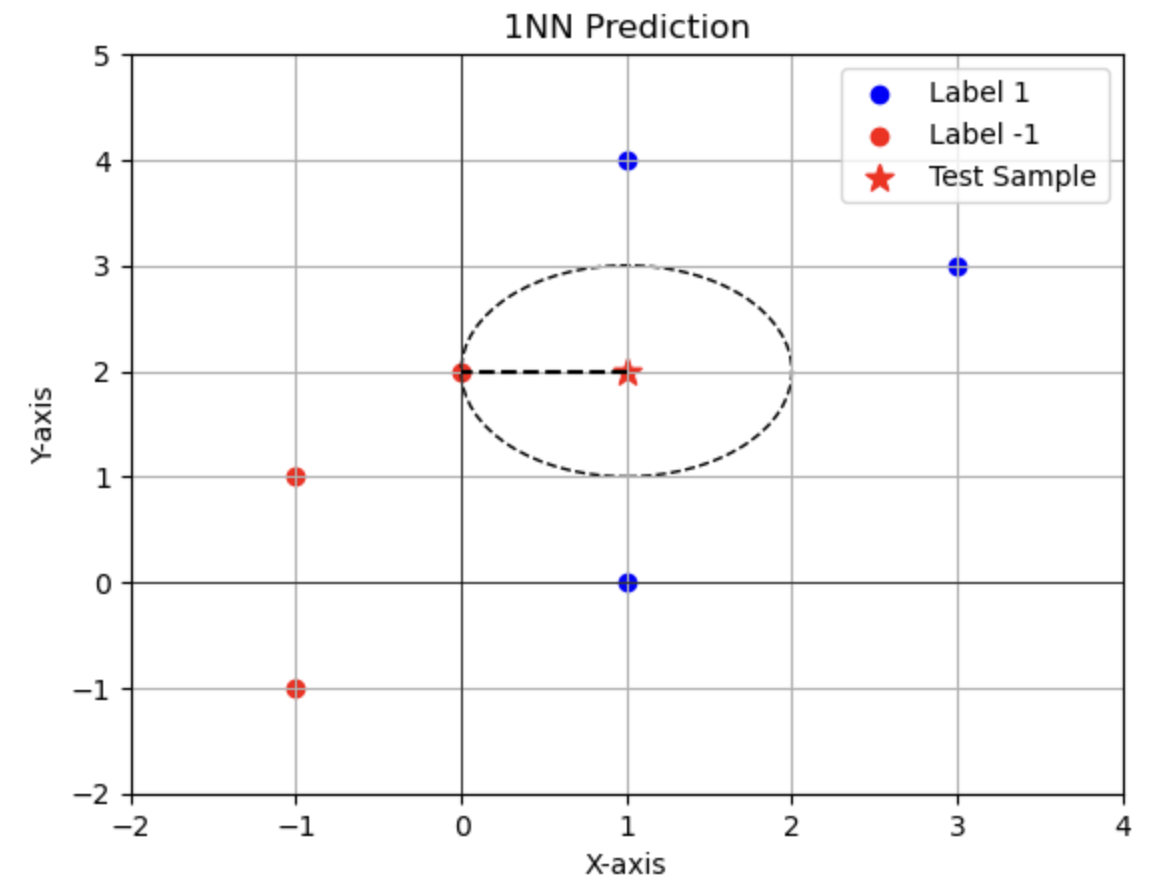
\includegraphics[width=\textwidth]{1NN.png}
        \caption{1-Nearest Neighbour}
        \label{fig:1nn}
    \end{minipage}\hfill
    \begin{minipage}{0.45\textwidth}
        \centering
        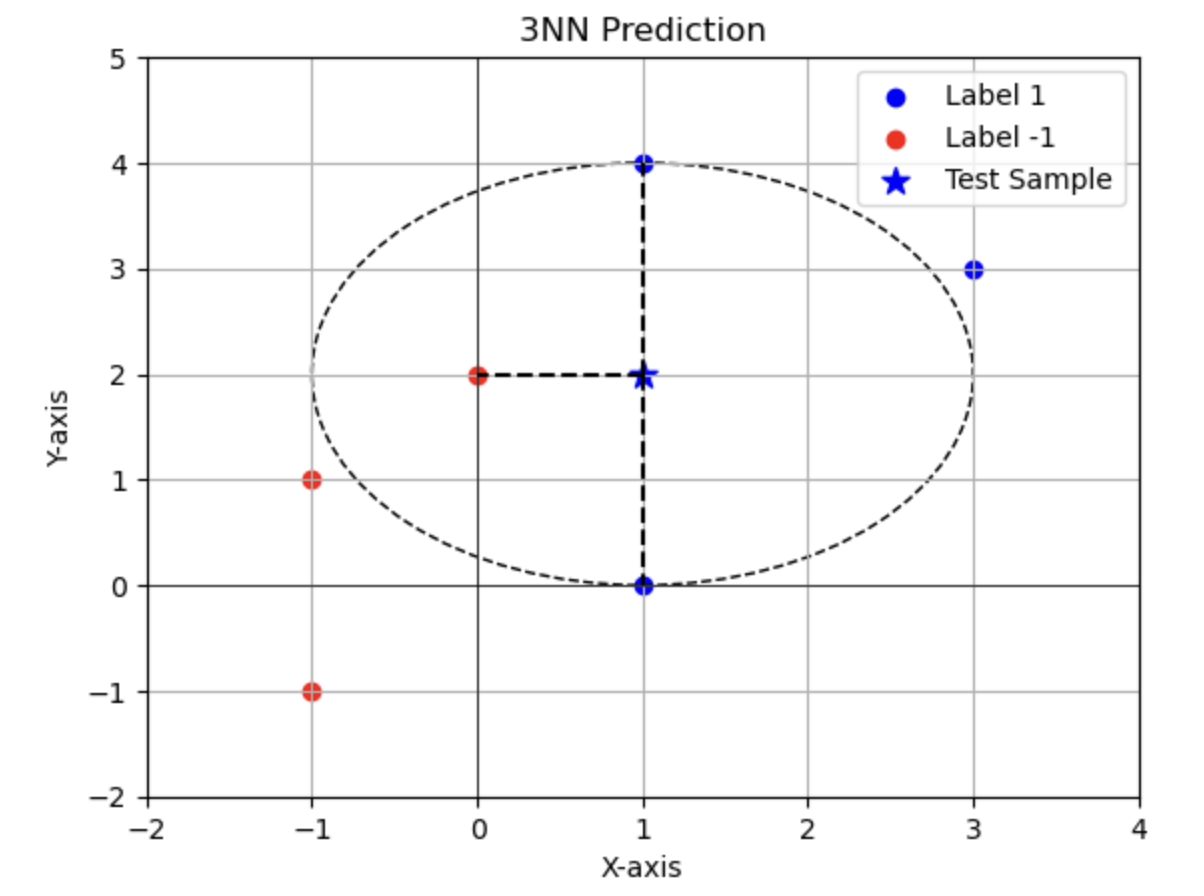
\includegraphics[width=\textwidth]{3NN.png}
        \caption{3-Nearest Neighbours}
        \label{fig:3nn}
    \end{minipage}
\end{figure}

In summary, the KNN algorithm for classification hinges on the concept of feature similarity, where the class of a new data point is determined based on the classes of its nearest neighbours in the feature space. This method's effectiveness is highly dependent on the choice of 'k' and the distance metric used, making these crucial parameters in KNN's application.


\subsubsection{Distance Metrics}
A critical aspect of the K-Nearest Neighbours (KNN) algorithm is the method used to calculate the distance between data points. The choice of the distance metric can significantly influence the performance of the algorithm. Different types of distance metrics are suited to different types of data and applications. Here, we explore some of the most commonly used distance metrics in KNN: \par

\textbf{Euclidean Distance} is the most commonly used metric in KNN. It is the "ordinary" straight-line distance between two points in Euclidean space. Given two points, \(p\) and \(q\), each with \(n\) dimensions, the Euclidean distance between \(p\) and \(q\) is defined as:

\[ d(p,q) = \sqrt{\sum_{i=1}^{n} (q_i - p_i)^2} \]

This distance is easy to understand and simple to compute, making it a natural choice for many applications. \par
\vspace{5pt}
\textbf{Manhattan Distance}, also known as City Block distance, is another useful metric, especially in urban settings. It is calculated as the sum of the absolute differences of their Cartesian coordinates. Formally, the Manhattan distance between two points \(p\) and \(q\) in \(n\)-dimensional space is:

\[ d(p,q) = \sum_{i=1}^{n} |q_i - p_i| \]

This metric can be more useful than the Euclidean distance in certain scenarios, particularly when data points have grid-like structures. \par
\vspace{5pt}
\textbf{Minkowski Distance} is a generalized metric form that includes both Euclidean and Manhattan distances as special cases. It is defined as:

\[ d(p,q) = (\sum_{i=1}^{n} |q_i - p_i|^p)^{1/p} \]

For \(p = 2\), it becomes the Euclidean distance, and for \(p = 1\), it is the Manhattan distance. This flexibility allows for more nuanced distance calculations, adaptable to different problem settings.


\subsubsection{Advantages and Limitations}
\textbf{Advantages of K-Nearest Neighbors}

\begin{itemize}
    \item \textbf{Simplicity and Intuitiveness:} KNN is very straightforward and easy to understand, making it an excellent choice for beginners in machine learning. The concept of "the nearest neighbors" is intuitive and doesn't require complex mathematical understanding.


    \item \textbf{Non-Parametric Nature:} Since KNN makes no assumptions about the underlying data distribution, it is suitable for non-linear data. This feature makes it adaptable to many real-world scenarios where the data distribution is unknown.

    \item \textbf{Adaptability to Complex Decision Boundaries:} KNN can capture complex decision boundaries depending on the value of \( k \).

    \item \textbf{Useful for Multiclass Problems:} KNN can handle multi-class settings without needing any adjustments, making it versatile in handling various classification tasks.
\end{itemize}

\textbf{Limitations of K-Nearest Neighbors}

\begin{itemize}
    \item \textbf{Computationally and Memory Intensive:} KNN can be computationally expensive, especially with large datasets, as it requires calculating the distance to all training samples for each prediction. Since the algorithm stores all the training data, memory consumption can be high for large datasets.

    \item \textbf{Sensitive to the Choice of \( k \) and Distance Metric:} The performance of KNN heavily relies on the choice of the number of neighbours (\( k \)) and the distance metric used. An inappropriate choice of \( k \) or distance metric can lead to very poor performance.

    \item \textbf{Vulnerable to Irrelevant Features:} KNN can be significantly affected by the presence of irrelevant or redundant features because all features contribute equally to the distance computation.

    \item \textbf{Curse of Dimensionality:} Its performance degrades as the number of features (dimensions) increases, due to the difficulty in calculating distances in high-dimensional spaces.

    \item \textbf{Performance Deterioration with Noisy Data:} KNN is sensitive to noise in the dataset, as noisy features can distort the true distance between points.

    \item \textbf{Class Imbalance Problems:} KNN can be biased towards the majority class in cases of class imbalance.

\end{itemize}
\subsubsection{Comparative Analysis with other ML Algorithms}
KNN's simplicity has been emphasised throughout this section, and it remains as its key strength when compared to other algorithms, such as Decision Trees and parametic methods. \par

\textbf{KNN vs. Decision Trees:} One of the fundamental differences between KNN and decision trees lies in their approach to learning and prediction. KNN is a typical example of lazy learning and instance-based learning. Unlike decision trees, which are eager learners, KNN does not build a model during the training phase. It simply stores the data and performs computations only at the time of prediction. This characteristic leads to different performance implications:

\begin{itemize}
    \item \textbf{Speed and Efficiency:} KNN can be slower at making predictions than decision trees, as it requires searching through the entire dataset for each query. In contrast, decision trees, once trained, can make predictions quickly by traversing the tree structure.
    \item \textbf{Memory Usage:} KNN is memory-intensive since it needs to store the entire dataset. Decision trees, after training, only require the tree structure for predictions, making them more memory-efficient.
    \item \textbf{Interpretability:} Decision trees offer a more interpretable model compared to KNN. The tree structure of decision trees provides clear rules and paths for decision-making, whereas KNN's predictions are based on the proximity to the nearest neighbors, which might not be as intuitive to understand.
\end{itemize}

\textbf{KNN vs. Parametric Methods:} KNN also differs significantly from parametric methods, such as linear regression or logistic regression. Parametric methods assume a specific form for the function that relates inputs to outputs and learn the parameters of this function from the training data. In contrast, KNN is a non-parametric method:

\begin{itemize}
    \item \textbf{Model Assumptions:} KNN makes no assumptions about the underlying data distribution, making it more flexible in handling a variety of data types and distributions. Parametric methods, with their fixed structure, can be limited in this aspect.
    \item \textbf{Complexity and Overfitting:} Parametric methods can be prone to overfitting or underfitting if the assumed model form is not well-aligned with the true underlying relationships. KNN, with its instance-based approach, can adapt more closely to the data but may also capture noise, leading to overfitting, especially with a small value of 'k'.
    \item \textbf{Scalability:} In terms of scalability, parametric methods often scale better to large datasets, as they summarize the data into a set of parameters. KNN's need to store and search through the entire dataset can become a bottleneck as data size increases.
\end{itemize}

\newpage
\subsection{Decision Trees}
Decision Trees are a prominent and widely used form of supervised machine learning algorithms, known for their simplicity, interpretability, and versatility in both classification and regression tasks. 
\subsubsection{Introduction}
Among machine learning algorithms, Decision Trees stand out for their straightforward yet powerful approach to classification tasks. Characterized by their tree-like structure, they simplify decision-making by breaking it down into a series of binary choices, leading to clear, actionable outcomes. This makes Decision Trees not only easy to interpret to anyone but also highly adaptable to various classification challenges. \par

They are quite capable when it comes to transforming complex decision boundaries into a sequence of simpler, binary splits. This process starts at the root node and progresses through various levels, with each node representing a decision point based on one of the input features. The branches, stemming from these nodes, lead to new decision points or leaf nodes, which represent the final classification decision. This hierarchical structure captures the essence of decision-making in a way that is both logical and intuitive. \par


Focusing on the \textbf{Classification and Regression Tree (CART)} algorithm within the Decision Tree family, this project explores its application in classification tasks. The CART algorithm distinguishes itself through its binary splitting approach, where each node is split into two child nodes, offering a balanced and manageable way to dissect the data. For classification tasks, CART employs \textbf{Gini Impurity} as a measure of split quality. Gini Impurity is a statistical metric that quantifies the likelihood of incorrect classification, making it an effective tool for evaluating the purity of the split. By minimizing Gini Impurity at each step, CART guides the decision-making process toward the most informative features in the dataset, with the aim of making accurate predictions on the target label. \par
This report delves into the inner workings of the CART algorithm, demonstrating how its structured approach to decision-making can be effectively harnessed for classification purposes. By implementing CART from scratch and utilizing Gini Impurity as the key criterion for data partitioning, the project aims to provide an insightful exploration into one of the more fundamental yet very versatile algorithms in the field of machine learning. \par

My primary source of material when researching how this algorithm functions was from the original text by Leo Breiman, Classification and Regression Trees~\cite{CARTBreiman} as well as a chapter within Machine Learning by Tom Mitchell~\cite[pp 52-80]{mitchell1997machine}.



\subsubsection{Fundamentals of Tree Mechanism}
Decision Trees operate on the fundamental principle of recursive partitioning of the dataset. This process begins at the root of the tree and involves splitting the data based on feature values. Each node in the tree represents a feature in the dataset, and the branches represent the outcomes of the decision made at that node. This leads to further subdivisions in the tree until a leaf node is reached, which provides the final prediction or classification.\par

The decision at each node is made based on certain criteria, typically aiming to maximize the homogeneity of the resultant subsets. For categorical features, the splits are based on the different categories, while for continuous features, the tree selects a threshold value for splitting the data. This recursive partitioning continues until certain stopping criteria are met, which prevents the tree from growing indefinitely and potentially overfitting the data.\par

My implementation uses this idea of a threshold with splitting continuous data, the approach to categorical data is to be implemented soon. \par

\begin{figure}[ht]
    \centering
    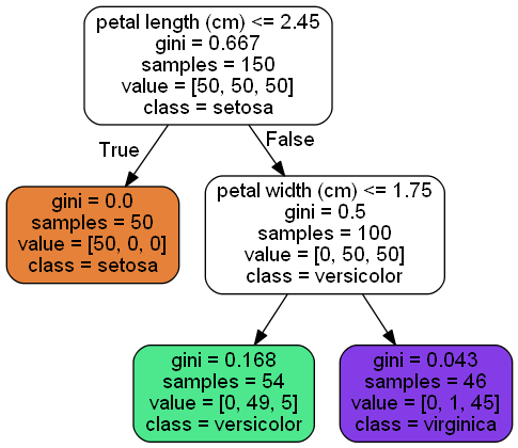
\includegraphics[width=0.4\textwidth]{sklearntree.png}
    \caption{Example of a tree using Gini}
    \label{fig:sklearntree}
\end{figure}

\subsubsection{Splitting, Stopping and Pruning Criteria}
In Decision Trees, the splitting criterion is a crucial aspect that determines how the data at each node is divided. The CART algorithm utilizes Gini Impurity as a primary measure for this purpose. Gini Impurity is a statistical metric used to quantify the "purity" of a node in the tree. The objective is to minimize this impurity, ensuring that after the split, the subsets are as homogeneous as possible with respect to the target variable. \par

\textbf{Gini Impurity:}
Gini Impurity measures the frequency at which any element of the dataset will be incorrectly labeled if it was randomly labeled according to the distribution of labels in the subset. The Gini Impurity for a set can be calculated using the formula:

\[ Gini(I) = 1 - \sum_{j} p_j^2 \]

Here, \( p_j \) represents the proportion of the samples that belong to class \( j \) in the set \( I \). This formula implies that a node is 'pure' (Gini = 0) if all its samples belong to a single class. \par
We can think of \(p\) as representing the probability that a single sample picked from this once belongs to its corresponding class. We find the probabilities for each class, square them and sum these squared values. We then subtract the sum found from 1 to find the impurity value. \par
The goal of the CART algorithm is to find splits that decrease the Gini Impurity the most across the nodes it creates.

The algorithm considers all possible thresholds for each feature and calculates the Gini Impurity for the resulting partitions. The feature and the threshold that result in the highest impurity reduction are chosen to split the node. This process is repeated recursively for each new child node.

\textbf{Stopping Criteria:}
The growth of the tree is regulated by stopping criteria to prevent overfitting. These criteria include:

\begin{itemize}
    \item Setting a maximum depth for the tree.
    \item A minimum number of samples required to split a node.
    \item A minimum number of samples required to be at a leaf node.
\end{itemize}
These parameters ensure that the tree does not grow too complex and models the data well without capturing noise.

\textbf{Pruning:}
After building the tree, pruning is performed to reduce its complexity and enhance its generalization abilities. Pruning involves cutting off branches of the tree that provide little predictive power. This is based on a cost-complexity trade-off, where smaller, simpler trees are preferred unless more complex trees provide substantial improvement in predictive ability. Pruning helps in reducing overfitting and improving the model's performance on unseen data. \par

By controlling the tree's growth and complexity through these mechanisms, Decision Trees can be a powerful tool for classification, striking a balance between fitting the training data well and maintaining good generalization to new, unseen data. \par

My implementation makes use of the Gini Impurity, using a fairly greedy strategy to find the most pure node at each split. It uses maximum depth, minimum number of samples at node and a node being totally pure as stopping criteria. Pruning is yet to be implemented, but it would be an ideal step to reduce overfitting in my implementation. 

\subsubsection{Advantages and Limitations}
\textbf{Advantages:}
\begin{itemize}
    \item \textbf{Interpretability:} Decision Trees are highly interpretable, making it easy to understand the decision-making process.
    \item \textbf{Handling Non-linear Relationships:} They can capture non-linear relationships between features and the target without the need for transformation.
    \item \textbf{No Need for Feature Scaling:} Decision Trees do not require normalization or standardization of features.
    \item \textbf{Versatility:} Capable of handling both numerical and categorical data.
\end{itemize}

\textbf{Limitations:}
\begin{itemize}
    \item \textbf{Overfitting:} Prone to overfitting, especially in cases with many features or complex structures.
    \item \textbf{Sensitivity to Variance in Data:} Small changes in the data can lead to different tree structures.
    \item \textbf{Biased with Imbalanced Data:} Can create biased trees if some classes dominate.
\end{itemize}

\subsubsection{Comparative Analysis with other ML Algorithms} 
Decision Trees, as a fundamental machine learning algorithm, have distinct characteristics when compared to other methods like K-Nearest Neighbors (KNN) and parametric approaches such as Support Vector Machines (SVMs) and Logistic Regression. Each algorithm has its strengths and weaknesses, making them suitable for different types of problems. \par
\vspace{5pt}
\textbf{Decision Trees vs. K-Nearest Neighbors:}
\begin{itemize}
\item \textbf{Learning Style:} While Decision Trees are eager learners that build a model based on the entire dataset before making predictions, KNN is a lazy learner that makes predictions using the dataset at the time of query. This difference impacts both training time and prediction time.
\item \textbf{Interpretability:} Decision Trees are highly interpretable, as they provide a clear decision-making path from root to leaf. KNN, on the other hand, bases its predictions on the proximity to the nearest neighbors, which might not be as intuitive.

\item \textbf{Sensitivity to Data Scale:} KNN is sensitive to the scale of data and requires feature scaling for optimal performance. Decision Trees are less sensitive to the scale of features.

\item \textbf{Handling Non-linear Data:} Both algorithms can handle non-linear data, but Decision Trees can be more effective in capturing complex relationships due to their hierarchical structure.
\end{itemize}

\textbf{Decision Trees vs. Parametric Methods:}
\begin{itemize}
\item \textbf{Interpretability:} Decision Trees excel in interpretability due to their clear, hierarchical decision-making structure. In contrast, parametric methods, especially complex ones like SVMs with non-linear kernels or logistic regression models with many predictors, can be less transparent due to their mathematical formulations.
\item \textbf{Handling Non-linear Relationships:} Decision Trees naturally adapt to non-linear relationships through their hierarchical structure of splits and decisions. Parametric methods, like logistic regression, can be extended to handle non-linearity using techniques such as feature transformation or kernel methods in SVMs.

\item \textbf{Flexibility in Data Types:} Decision Trees are versatile in handling both categorical and numerical data directly. Parametric methods typically require numerical input, often necessitating additional steps such as one-hot encoding for categorical data.

\item \textbf{Robustness to Overfitting:} Both Decision Trees and parametric methods can overfit data. Decision Trees can grow overly complex, capturing noise, but pruning helps mitigate this. Parametric methods, particularly those with many parameters, are also prone to overfitting, but regularization techniques can help.

\item \textbf{Scalability and Efficiency:} Parametric methods, like logistic regression, can be computationally efficient for large datasets, summarizing information into parameters. Decision Trees, however, may become less efficient with large datasets or feature spaces, especially if the tree grows very deep or complex.
\end{itemize}




\newpage

\subsection{Logistic Regression}
When selecting a third algorithm, I wanted to introduce a parametric model. The previous two algorithms are non-parametric and I was curious about implementing something different in this regard, and I felt it would make the comparison of performances interesting. Logistic regression also seemed like a highly relevant algorithm in discussions and is quite strongly associated within the mechanism of neural networks, which seemed useful for me to dig into. \par
Logistic Regression is a fundamental statistical model and a key algorithm in the field of machine learning, particularly renowned for its effectiveness in binary classification tasks. This section delves into the core concepts, mathematical foundations, and practical aspects of logistic regression, highlighting its significance in predictive modelling.\par

\subsubsection{Overview}
Logistic Regression is a supervised learning algorithm that finds extensive application in various domains, such as medical diagnosis, marketing, and finance, where the goal is to predict a binary outcome. Unlike linear regression, which aims to predict continuous values, logistic regression focuses on estimating the probability of an instance belonging to a particular class. By learning a set of weights and a bias term from labeled training data, logistic regression constructs a model capable of making probabilistic predictions on unseen instances. \par

At the heart of logistic regression lies the logistic function, also known as the sigmoid function. This mathematical function takes a linear combination of input features and maps it to a probability value between 0 and 1. By applying a threshold to this probability, typically set at 0.5, the model can classify instances into one of two classes. The elegance and simplicity of logistic regression, combined with its ability to provide interpretable results, have solidified its position as a go-to algorithm for binary classification tasks. \par

Despite its name, logistic regression is inherently a classification algorithm rather than a regression method. The term "regression" in its name stems from the fact that it estimates the parameters of a logistic function, which is a continuous function, to model the relationship between the input features and the binary outcome. This distinguishes logistic regression from other classification algorithms that directly output class labels without providing probability estimates. \par

In the following subsections, we will explore the logistic function in detail, understand how the model parameters are estimated using gradient descent, discuss the advantages and limitations of logistic regression, and extend the concept to multi-class classification through softmax regression. By the end of this section, readers will have a comprehensive understanding of logistic regression and its practical applications in solving binary classification problems.

During research, I actually found one of the most useful resources for this was Aurelien Geron's Hands-On with Machine Learning~\cite{geron2017hands-on}. This book is very well structured and aided in understanding good machine learning practices too.

\subsubsection{The Logistic Function}
The logistic function, also known as the sigmoid function, is the cornerstone of logistic regression. It is a smooth, S-shaped curve that maps any real-valued input to a value between 0 and 1. Mathematically, the logistic function is defined as:

\[ \sigma(z) = \frac{1}{1 + e^{-z}} \]

where $\sigma(z)$ represents the logistic function, and $z$ is the input, which is typically a linear combination of the input features and their corresponding weights. The input $z$ is calculated as:

\[ z = w_0 + w_1x_1 + w_2x_2 + \ldots + w_nx_n \]

where $w_0$ is the bias term, $w_1, w_2, \ldots, w_n$ are the weights associated with the input features $x_1, x_2, \ldots, x_n$, respectively. \par

The logistic function possesses several properties that make it suitable for modelling probabilities:

\begin{itemize}
\item \textbf{Bounded Output:} The output of the logistic function is always between 0 and 1, making it interpretable as a probability.
\item \textbf{Monotonicity:} As the input $z$ increases, the output of the logistic function also increases monotonically. This property ensures that the model's predictions are consistent with the notion that higher values of $z$ correspond to a higher probability of belonging to the positive class.
\item \textbf{Differentiability:} The logistic function is differentiable at every point, which is crucial for the optimization process during model training.
\end{itemize}

In logistic regression, the output of the logistic function is interpreted as the probability of an instance belonging to the positive class (usually denoted as class 1). By setting a threshold, typically at 0.5, the model can classify instances based on their predicted probabilities. If the predicted probability is greater than or equal to the threshold, the instance is classified as belonging to the positive class; otherwise, it is classified as belonging to the negative class (usually denoted as class 0). \par

The logistic function's ability to convert a linear combination of input features into a probability value is the key reason why it is used in logistic regression. It allows the model to capture the non-linear relationship between the input features and the binary outcome while providing a meaningful interpretation of the model's predictions. \par

\subsubsection{Model Estimation via Gradient Descent}
Estimating the parameters (weights and bias) of the logistic regression model is a crucial step in building a well-performing classifier. The goal is to find the set of parameters that best fits the training data, minimizing the discrepancy between the predicted probabilities and the actual class labels. This is typically achieved through an optimization process called gradient descent. \par

Gradient descent is an iterative algorithm that minimizes a cost function by adjusting the model parameters in the direction of steepest descent. In logistic regression, the cost function used is the log loss, also known as binary cross-entropy. The log loss quantifies the dissimilarity between the predicted probabilities and the true class labels, and it is defined as:

\[ J(w) = -\frac{1}{m} \sum_{i=1}^{m} [y^{(i)} \log(\hat{y}^{(i)}) + (1 - y^{(i)}) \log(1 - \hat{y}^{(i)})] \]

where $J(w)$ is the cost function, $m$ is the number of training instances, $y^{(i)}$ is the true class label of the $i$-th instance (either 0 or 1), $\hat{y}^{(i)}$ is the predicted probability of the $i$-th instance belonging to class 1, and $w$ represents the model parameters (weights and bias). \par

To minimize the cost function, gradient descent iteratively updates the model parameters by taking steps in the direction of the negative gradient. The update rule for the weights and bias is as follows:

\[ w_j := w_j - \alpha \frac{\partial J(w)}{\partial w_j} \]

where $w_j$ is the $j$-th weight, $\alpha$ is the learning rate (a hyperparameter that controls the step size), and $\frac{\partial J(w)}{\partial w_j}$ is the partial derivative of the cost function with respect to the $j$-th weight. The partial derivative can be calculated as:

\[ \frac{\partial J(w)}{\partial w_j} = \frac{1}{m} \sum_{i=1}^{m} (\hat{y}^{(i)} - y^{(i)}) x_j^{(i)} \]

where $x_j^{(i)}$ is the $j$-th feature of the $i$-th instance. \par

The learning rate $\alpha$ plays a crucial role in the convergence of gradient descent. A small learning rate leads to slower convergence, while a large learning rate may cause the algorithm to overshoot the minimum and diverge. The choice of learning rate is often determined through experimentation or adaptive methods. \par

Gradient descent iteratively updates the model parameters until a stopping criterion is met, such as reaching a maximum number of iterations or achieving a sufficiently small change in the cost function. \par

To prevent overfitting and improve the model's generalization ability, regularization techniques can be incorporated into the cost function. L2 regularization, also known as Ridge regularization, adds a penalty term to the cost function that discourages large weight values. The modified cost function with L2 regularization is:

\[ J(w) = -\frac{1}{m} \sum_{i=1}^{m} [y^{(i)} \log(\hat{y}^{(i)}) + (1 - y^{(i)}) \log(1 - \hat{y}^{(i)})] + \frac{\lambda}{2m} \sum_{j=1}^{n} w_j^2 \]

where $\lambda$ is the regularization parameter that controls the strength of regularization, and $n$ is the number of features. The regularization term penalizes large weight values, encouraging the model to learn simpler and more generalizable patterns. \par

By iteratively updating the model parameters using gradient descent and incorporating regularization, logistic regression can effectively estimate the optimal weights and bias that minimize the cost function and achieve accurate binary classification.

\subsubsection{Advantages and Limitations}

Logistic regression offers several advantages that make it a popular choice for binary classification tasks:

\begin{itemize}
  \item \textbf{Interpretability:} Logistic regression provides interpretable results by assigning weights to each input feature. The magnitude and sign of the weights indicate the importance and direction of the relationship between the feature and the binary outcome. This interpretability is particularly valuable in domains such as medicine and finance, where understanding the factors contributing to the prediction is crucial.

  \item \textbf{Probabilistic Output:} Unlike some other classification algorithms that directly output class labels, logistic regression provides probability estimates. The predicted probability of an instance belonging to the positive class can be used to assess the confidence of the prediction and make informed decisions based on different threshold values.

  \item \textbf{Efficiency:} Logistic regression is computationally efficient and can handle large datasets. The training process, which involves optimizing the model parameters using gradient descent, is relatively fast compared to more complex algorithms. This efficiency makes logistic regression suitable for real-time applications and scenarios where quick predictions are required.

  \item \textbf{Robustness:} Logistic regression is relatively robust to outliers and can handle noise in the data to some extent. The logistic function, being a smooth and continuous function, helps to mitigate the impact of extreme values on the model's predictions.
\end{itemize}

However, logistic regression also has some limitations:

\begin{itemize}
  \item \textbf{Linearity Assumption:} Logistic regression assumes a linear relationship between the input features and the log-odds of the binary outcome. If the relationship is highly non-linear, logistic regression may not capture the underlying patterns effectively. In such cases, feature engineering techniques or more advanced algorithms, such as decision trees or neural networks, may be more appropriate.

  \item \textbf{Feature Interactions:} Logistic regression does not inherently capture interactions between input features. If there are significant interactions or multiplicative effects among the features, they need to be explicitly included in the model by creating interaction terms. Identifying and incorporating relevant interaction terms can be challenging and may require domain knowledge or extensive feature engineering.

  \item \textbf{Imbalanced Data:} Logistic regression can be sensitive to class imbalance, where one class has significantly more instances than the other. In such cases, the model may be biased towards the majority class, leading to poor performance on the minority class. Techniques such as oversampling, undersampling, or class weighting can be used to address class imbalance and improve the model's performance.

  \item \textbf{High-Dimensional Data:} Logistic regression may struggle with high-dimensional data, where the number of input features is much larger than the number of instances. In such scenarios, the model may overfit the training data and perform poorly on unseen instances. Regularization techniques, such as L1 or L2 regularization, can help mitigate overfitting, but feature selection or dimensionality reduction techniques may also be necessary to handle high-dimensional data effectively.
\end{itemize}

Despite these limitations, logistic regression remains a valuable tool in the machine learning practitioner's toolkit. Its simplicity, interpretability, and efficiency make it a good starting point for binary classification tasks. However, it is essential to understand its assumptions and limitations and consider alternative algorithms when dealing with non-linear relationships, feature interactions, imbalanced data, or high-dimensional datasets.

\subsection{Softmax Regression}
Logistic regression is inherently designed for binary classification, which posed a challenge for me since I had been using my previous two algorithms on multi-class datasets and had no intention of narrowing the task to binary classification tasks. Although traditional logistic regression is constrained to this task, it can be extended to handle multi-class classification problems through the use of softmax regression. \par

Softmax regression, also known as multinomial logistic regression, is a generalization of logistic regression that allows for the prediction of multiple classes simultaneously. \par

In softmax regression, the goal is to estimate the probabilities of an instance belonging to each of the possible classes. Instead of a single logistic function, softmax regression uses the softmax function, which is a multi-class generalization of the logistic function. The softmax function takes a vector of real-valued scores and transforms them into a vector of probabilities, where each probability represents the likelihood of the instance belonging to a particular class. \par

\subsubsection{Softmax Function and Model Estimation}
The softmax function is defined as follows:

\[ \sigma(\mathbf{z})_i = \frac{e^{z_i}}{\sum_{j=1}^{K} e^{z_j}} \text{ for } i = 1, \dots, K \]

where $\mathbf{z} = (z_1, \dots, z_K)$ is a vector of real-valued scores for each of the $K$ classes, and $\sigma(\mathbf{z})_i$ represents the probability of the instance belonging to class $i$. The softmax function ensures that the probabilities sum up to 1, making them a valid probability distribution over the classes. \par

In softmax regression, the scores $\mathbf{z}$ are typically obtained by a linear combination of the input features and the corresponding weights for each class:

\[ z_i = \mathbf{w}_i^\top \mathbf{x} + b_i \text{ for } i = 1, \dots, K \]

where $\mathbf{w}_i$ is the weight vector for class $i$, $\mathbf{x}$ is the input feature vector, and $b_i$ is the bias term for class $i$. \par

The model parameters (weights and biases) are estimated by minimizing the cross-entropy loss function, which measures the dissimilarity between the predicted probabilities and the true class labels. The cross-entropy loss for a single instance is defined as:

\[ L(\mathbf{y}, \hat{\mathbf{y}}) = -\sum_{i=1}^{K} y_i \log(\hat{y}_i) \]

where $\mathbf{y} = (y_1, \dots, y_K)$ is the one-hot encoded true class label vector, with $y_i = 1$ if the instance belongs to class $i$ and $y_i = 0$ otherwise, and $\hat{\mathbf{y}} = (\hat{y}_1, \dots, \hat{y}_K)$ is the vector of predicted probabilities obtained from the softmax function. \par

To minimize the cross-entropy loss and estimate the model parameters, gradient descent is used, similar to logistic regression. The gradients of the loss with respect to the weights and biases are computed, and the parameters are updated iteratively until convergence. \par

L2 regularization can also be incorporated into the loss function to prevent overfitting. The regularization term penalizes large weight values, encouraging the model to learn simpler and more generalizable patterns. The modified loss function with L2 regularization is:

\[ L(\mathbf{y}, \hat{\mathbf{y}}) = -\sum_{i=1}^{K} y_i \log(\hat{y}_i) + \frac{\lambda}{2} \sum_{i=1}^{K} \|\mathbf{w}_i\|^2 \]

where $\lambda$ is the regularization parameter that controls the strength of regularization. \par

\subsubsection{Gradient Descent in Softmax Regression}
The gradient descent algorithm in softmax regression follows a similar approach to logistic regression. The goal is to iteratively update the model parameters (weights and biases) in the direction of the negative gradient of the loss function. \par

The gradients of the cross-entropy loss with respect to the weights and biases for a single instance can be computed as:

\[ \frac{\partial L}{\partial \mathbf{w}_i} = (\hat{y}_i - y_i) \mathbf{x} + \lambda \mathbf{w}_i \]
\[ \frac{\partial L}{\partial b_i} = \hat{y}_i - y_i \]

where $\hat{y}_i$ is the predicted probability for class $i$, $y_i$ is the true label for class $i$ (0 or 1), $\mathbf{x}$ is the input feature vector, and $\lambda$ is the regularization parameter. \par

The update rules for the weights and biases are:

\[ \mathbf{w}_i := \mathbf{w}_i - \alpha \frac{\partial L}{\partial \mathbf{w}_i} \]
\[ b_i := b_i - \alpha \frac{\partial L}{\partial b_i} \]

where $\alpha$ is the learning rate that determines the step size of the updates. \par

The gradient descent algorithm iterates over the training instances, computing the gradients and updating the parameters until convergence. The convergence can be determined based on a maximum number of iterations or a minimum change in the loss function. \par

Practical considerations in softmax regression include:
\begin{itemize}
  \item \textbf{Learning Rate:} Choosing an appropriate learning rate is crucial for convergence. A too-small learning rate may result in slow convergence, while a too-large learning rate may cause the algorithm to overshoot the minimum and diverge. Techniques such as learning rate scheduling or adaptive learning rates can be used to improve convergence.

  \item \textbf{Initialization:} Initializing the weights and biases with appropriate values can help the algorithm converge faster. Common initialization techniques include random initialization with small values or using pre-trained weights from a related task.

  \item \textbf{Batch vs. Stochastic Gradient Descent:} Gradient descent can be performed in batch mode, where the gradients are computed over the entire training set, or in stochastic mode, where the gradients are computed for individual instances or small batches. Stochastic gradient descent often converges faster and can handle large datasets more efficiently.

  \item \textbf{Regularization:} Adjusting the regularization parameter $\lambda$ helps control the trade-off between fitting the training data and generalizing to unseen data. Higher values of $\lambda$ lead to stronger regularization and can help prevent overfitting.
\end{itemize}

By iteratively updating the model parameters using gradient descent and incorporating regularization, softmax regression can effectively estimate the class probabilities and make accurate predictions in multi-class classification tasks.

\newpage


\section{Model Evaluation Techniques}
In this section, we'll cover concepts and techniques used to evaluate the performance of these models we've undertaken.
\subsection{Bias And Variance}
In the realm of machine learning, two key concepts that play a pivotal role in model performance are bias and variance. These terms describe the types of errors a machine learning model might encounter and are crucial in understanding the trade-offs in different model choices. \par

\textbf{Bias} refers to the error introduced by approximating a real-world problem, which may be complex, with a too-simplified model. In essence, bias measures how far off, on average, a model's predictions are from the actual values. High bias can cause a model to miss relevant relations between features and target outputs (underfitting), leading to poor performance on both training and unseen data. \par

\textbf{Variance}, on the other hand, refers to the model's sensitivity to fluctuations in the training dataset. A model with high variance pays a lot of attention to training data and can capture noise present in the dataset rather than the intended outputs (overfitting). Such a model performs well on its training data but poorly on any unseen data. \par

The relationship between bias and variance is a balancing act and is often referred to as \textbf{the bias-variance tradeoff}. Minimizing one typically leads to an increase in the other. For instance, a highly complex model (low bias) might fit the training data too closely, capturing noise and anomalies (high variance). Conversely, a too-simple model (high bias) might fail to capture important patterns, leading to poor prediction accuracy. \par

An ideal model is one that achieves a good balance between bias and variance, ensuring it performs well on both the training data and unseen data. This balance is often achieved through model selection, feature engineering, and tuning of model parameters. \par

\textbf{Accuracy} in this context is a measure of a model's overall correctness in classifying data or predicting outcomes. However, it's essential to consider that a highly accurate model on training data may not necessarily generalize well to new, unseen data if it has high variance. \par


\subsection{Hold-Out Test Set}
Quite a central process when evaluating machine learning models involves dividing our data into training and test sets. The test set, and this particular process, is sometimes more formally known as a \textbf{Hold-Out Test Set}. This technique involves partitioning the dataset into two segments: one that is used to train the model and another that is used to test and evaluate its performance. \par

\textbf{Training Set:} This is the portion of the dataset used to train the model. The training set allows the algorithm to identify patterns, learn the relationships between features and the target variable, and build the model. The size of the training set can significantly influence the model’s learning, with larger training sets generally providing more comprehensive learning opportunities.

\textbf{Test Set:} Once the model is trained, it is essential to evaluate its performance on data it hasn't seen before. This is where the testing set comes in. It is a separate portion of the dataset not used during the training phase. By assessing the model's performance on the testing set, we get a sense of how well the model generalizes to new, unseen data. \par

All in all, this is rather simple to implement and undertake - but the performance we find can heavily vary depending on the splits of our data. So our assessment can have a lot of variability. This issue is directly addressed with the following technique. 

\subsection{Cross-Validation}
While the Hold-Out Test Set method provides an initial assessment of a model's generalization capability, it can lead to variability in performance evaluation due to different splits of the data. To address this issue and obtain a more robust evaluation, the technique of Cross-Validation is employed - and is generally utilised to evaluate a classification model's performance in making accurate predictions. \par

\textbf{Cross-validation} is a resampling procedure used to evaluate machine learning models on a limited data sample. The fundamental idea behind this technique is to divide the entire dataset into multiple subsets and then systematically use different subsets for training and testing the model. This approach ensures that every data point is used for both training and testing, providing a comprehensive assessment of the model's performance. \par

Essentially, we're carrying on this idea of splitting the dataset into training and test sets, and we're repeating it in several different segments or subsets of the dataset. We could name these several test sets as 'folds'. \par

With this in mind, we find that the most common form of Cross-Validation is \textbf{K-fold Cross-Validation}. In this method, the dataset is randomly partitioned into 'k' equal-sized folds. For each iteration, one of the 'k' subsets is used as the test set, and the remaining 'k-1' subsets are put together to form a training set. The model is then trained on this training set and validated on the test set. This process is repeated 'k' times, with each of the 'k' subsets used exactly once as the test set. The results from all 'k' iterations are then averaged to produce a single estimation. \par

\begin{figure}[ht]
    \centering
    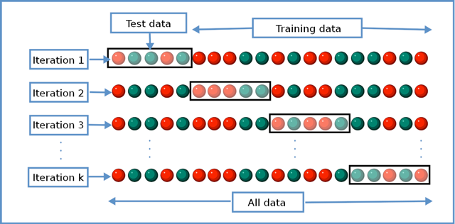
\includegraphics[width=0.6\textwidth]{KFolds.png}
    \caption{Illustration of K-fold Cross-Validation}
    \label{fig:kfolds}
\end{figure}

In this project's implementation, we incorporate functions that return a list of accuracy values calculated on each fold, as well as the average of this list of values. \par

Another notable variant of Cross-Validation is \textbf{Leave-One-Out Cross-Validation} (LOOCV). In LOOCV, the 'k' in k-fold Cross-Validation is set equal to the number of observations in the dataset. This means that for a dataset with N observations, the model is trained N times, each time using all observations except one for training and the left-out observation for testing. \par

LOOCV is particularly useful when dealing with small datasets, as it maximizes the amount of data used for training the model. Each iteration provides a test on a unique single data point, offering a thorough exploration of the model's performance across the entire dataset. However, LOOCV can be highly computationally intensive for larger datasets, as it requires the model to be retrained from scratch for each of the N iterations. I've found this to be the case in my implementation, especially for the tree model implementation.



\subsection{Metrics} \label{withinscopefinish}

Various metrics are used to assess different aspects of a model's performance, with each metric offering unique insights. In this project, we focus on several key metrics: Accuracy, Precision, Specificity, Recall, and the F1 Score. \par

\textbf{Accuracy} was introduced earlier as a measure of a model's overall correctness. It is the ratio of correctly predicted instances to the total instances in the dataset. While accuracy is straightforward and widely used, it may not always be the best indicator of a model's performance, especially in cases where the data is imbalanced. \par

\[ \text{Accuracy} = \frac{\text{True Positives} + \text{True Negatives}}{\text{Total Instances}} \]

\textbf{Precision} refers to the proportion of positive identifications that were actually correct. It is calculated as the ratio of true positives (correct positive predictions) to the sum of true and false positives. Precision is a critical measure in scenarios where the cost of a false positive is high. \par

\[ \text{Precision} = \frac{\text{True Positives}}{\text{True Positives} + \text{False Positives}} \]

\textbf{Specificity}, also known as True Negative Rate, measures the proportion of actual negatives that are correctly identified by the model. It is calculated as the ratio of true negatives (correct negative predictions) to the sum of true negatives and false positives. Specificity is important when the cost of false positives is high. \par

\[ \text{Specificity} = \frac{\text{True Negatives}}{\text{True Negatives} + \text{False Positives}} \]

\textbf{Recall}, also known as Sensitivity or True Positive Rate, measures the proportion of actual positives that were correctly identified. It is calculated as the ratio of true positives to the sum of true positives and false negatives. Recall becomes a key metric when the cost of a false negative is high. \par

\[ \text{Recall} = \frac{\text{True Positives}}{\text{True Positives} + \text{False Negatives}} \]

\textbf{F1 Score} is the harmonic mean of Precision and Recall. It provides a single metric that balances both the concerns of precision and recall in one number. The F1 Score is particularly useful when we need a balance between precision and recall and there is an uneven class distribution (as is often the case in real-world scenarios). \par

\[ \text{F1 Score} = 2 \cdot \frac{\text{Precision} \cdot \text{Recall}}{\text{Precision} + \text{Recall}} \]

\subsection{Grid Search}
Grid search isn't exactly a model evaluation technique per se, but rather a method utilised during the tuning and optimisation of our model via the adjustment of our hyperparameters. I decided to write a small section describing this process of hyperparameter optimisation as it takes up a significant role in my final implementation of the project.\par
Hyperparameters are the adjustable settings of a machine learning algorithm that are set prior to the learning process. These parameters are not learned from the data but are instead specified by the user. Examples of hyperparameters include the learning rate, regularization strength, number of hidden layers in a neural network, or the depth of a decision tree. The choice of hyperparameter values can significantly impact the performance of a machine learning model. Therefore, finding the optimal combination of hyperparameters is crucial for achieving the best possible results. \par

Hyperparameter optimization is the process of systematically searching for the best hyperparameter values that maximize a model's performance on a given task. It involves defining a search space for each hyperparameter and exploring different combinations of values within that space. The objective is to find the hyperparameter configuration that yields the highest performance metric, such as accuracy or F1 score, on a validation set. \par

Grid Search is a straightforward and widely used technique for hyperparameter optimization. It involves specifying a discrete set of values for each hyperparameter and exhaustively evaluating all possible combinations of these values. The process can be visualized as a grid, where each cell represents a unique combination of hyperparameter values. \par

\begin{figure}[ht]
    \centering
    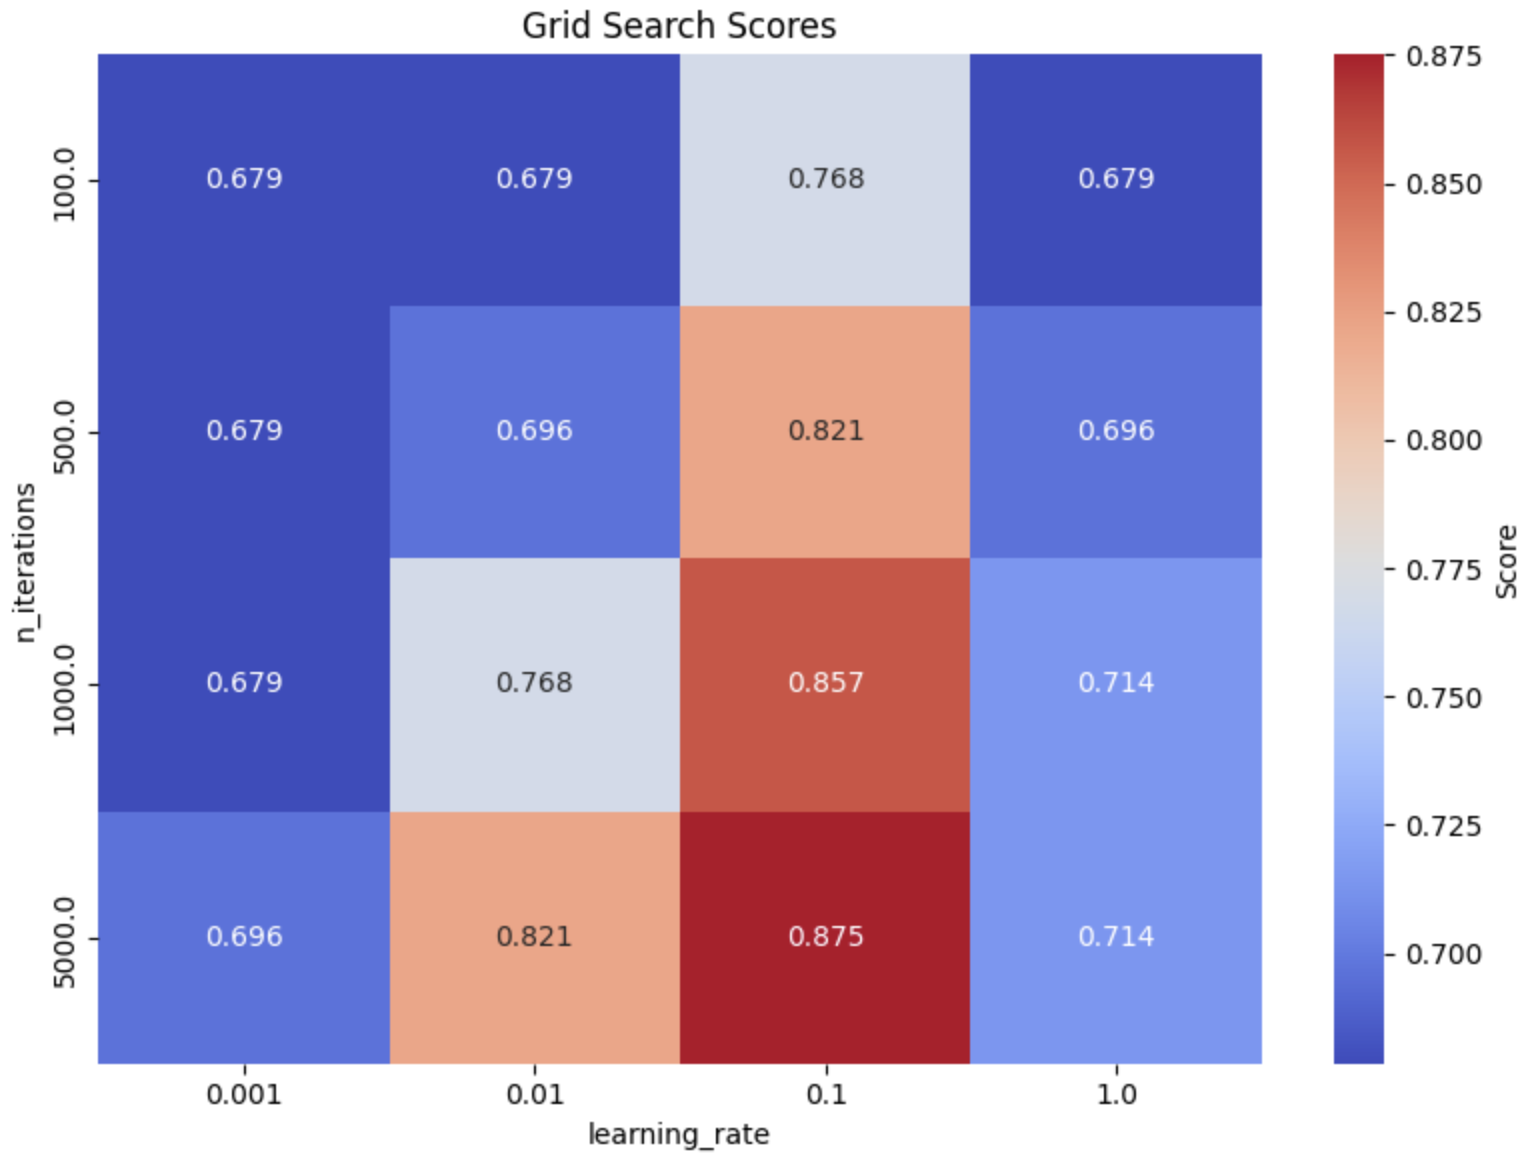
\includegraphics[width=0.6\textwidth]{grid-search.png}
    \caption{Example of Grid Search Results while tuning Softmax Regression, where number of iterations of gradient descent and the learning rate are hyperparameters. Taken from Notebook 10.}
    \label{fig:grid-search}
\end{figure}

The main advantage of Grid Search is its simplicity and completeness. By exploring all possible combinations, it guarantees finding the optimal hyperparameter configuration within the specified search space. However, this exhaustive search can be computationally expensive, especially when dealing with a large number of hyperparameters or a wide range of values. As the number of hyperparameters and their possible values increase, the number of combinations grows exponentially, making Grid Search infeasible for high-dimensional search spaces.\par

Despite its limitations, Grid Search remains a valuable technique for hyperparameter optimization, particularly when the search space is relatively small, and the computational resources are sufficient. It provides a systematic and interpretable way to tune hyperparameters and can serve as a baseline for more advanced optimization techniques.\par

\newpage
\section{Professional Issues: Bias}
The rapid advancement of machine learning and artificial intelligence (AI) has revolutionized various aspects of our lives. However, as the influence of these technologies grows, it is crucial to acknowledge and address the issue of bias in AI systems. Bias, whether intentional or unintentional, can have profound and far-reaching consequences on individuals and society as a whole. \par

This section aims to explore the types of bias that can occur in machine learning and AI, examine their impacts on society, discuss how bias was considered in the context of this project, and highlight the importance of addressing bias as an engineer moving forward in the field. By acknowledging and actively working towards mitigating bias, we can strive to create more equitable and trustworthy AI systems that benefit everyone. \par

The presence of bias in AI is a complex issue that can arise from various sources, including biased data, algorithmic design choices, and human prejudices. When left unchecked, biased AI systems can perpetuate and amplify existing societal biases, leading to unfair and discriminatory outcomes. As AI becomes more integrated into decision-making processes across industries, the potential for biased outcomes becomes increasingly concerning. \par

In the following sections, we will delve deeper into the types of bias, their societal impacts, and the steps taken to address bias in this project. Moreover, we will discuss the importance of cultivating a deep understanding of the ethical implications of AI and prioritizing fairness and transparency as an engineer in this field. \par

\subsection{Types of Bias}
Bias in machine learning and AI can manifest in various forms, each with its own unique characteristics and challenges. The three main categories of bias are:
\subsubsection{Data Bias
}Data bias refers to the biases present in the data used to train machine learning models. It can occur due to issues in data collection, labelling, or representation. Two common forms of data bias are selection bias, where the training data is not representative of the intended population, and measurement bias, where the data collected is inaccurate or inconsistent.

\subsubsection{Algorithmic Bias
}Algorithmic bias refers to the biases introduced by the design choices and assumptions made during the development of machine learning algorithms. These biases can arise from the selection of features, the choice of model architecture, or the optimization objectives. For example, if a model is optimized solely for accuracy without considering fairness metrics, it may make predictions that are biased against certain groups.

\subsubsection{Human Bias}
Human bias encompasses the biases introduced by the individuals involved in the development and deployment of AI systems. These biases can stem from personal experiences, cultural backgrounds, or societal prejudices and can influence various stages of the AI development process, from problem formulation to model evaluation and interpretation.

These types of bias are not mutually exclusive and can interact with each other, making it challenging to identify and mitigate them. A comprehensive approach that addresses bias at every stage of the AI development process is crucial.

\subsection{Bias and Society}
Biased AI systems can have significant negative impacts on society. They can perpetuate and amplify existing societal biases, leading to unfair and discriminatory outcomes. In domains such as hiring~\cite{amazon_hiring}, lending~\cite{credit_Score_bias}, and criminal justice~\cite{wrong_arrest_bias}, biased AI algorithms can result in the denial of opportunities, the reinforcement of historical inequalities, and the erosion of trust in technology. For example, a biased hiring algorithm may systematically discriminate against qualified candidates based on their gender, race, or age, thus perpetuating workplace inequalities. Similarly, biased AI systems in the criminal justice system can lead to disproportionate and unjust outcomes for certain communities. As AI becomes more prevalent in decision-making processes, it is crucial to address bias to ensure fairness and equal treatment for all individuals.

\subsection{Lessons}
\subsubsection{Within This Project}
In the context of this project, which involves the comparative analysis of machine learning algorithms, it is essential to acknowledge and address potential biases. This includes carefully examining the datasets used for training and testing, ensuring they are representative and diverse. Preprocessing techniques, such as handling missing data and encoding categorical variables, should be applied consistently to avoid introducing biases. When selecting models, it is important to consider not only their predictive performance but also their interpretability and fairness. Evaluation metrics should go beyond accuracy and include fairness metrics to assess the models' performance across different subgroups. However, addressing bias in machine learning projects can be challenging, as it requires continuous vigilance and iteration. Limitations, such as the availability of diverse data and the complexity of fairness metrics, should be acknowledged and documented. \par
\subsubsection{In My Career Ahead}
As an engineer working with machine learning and AI, it is crucial to prioritize fairness and ethics throughout the development process. This involves being aware of potential biases at every stage, from data collection and preprocessing to model selection and evaluation. Engaging in interdisciplinary collaboration, particularly with domain experts and stakeholders from diverse backgrounds, can help identify and mitigate biases. Continuously learning about best practices for fair and ethical AI, such as techniques for bias detection and mitigation, is essential for staying updated in this rapidly evolving field. As an engineer, I have a responsibility to develop AI systems that are transparent, accountable, and aligned with societal values. By proactively addressing bias and prioritizing fairness, I can contribute to building trust in AI and ensuring its benefits are distributed equitably. \par

Bias in machine learning and AI is a critical issue that demands attention and action from researchers, engineers, and society as a whole. By understanding the different types of bias and their impacts on society, we can work towards developing fair and unbiased AI systems. In the context of this project, acknowledging and addressing potential biases in datasets, algorithms, and evaluation metrics is crucial for ensuring the validity and fairness of the comparative analysis. As an engineer embarking on a career in this field, cultivating a strong ethical foundation and prioritizing fairness and transparency in the development and deployment of AI systems is essential. By actively addressing bias and striving for equity, we can harness the power of AI to benefit society as a whole and build a future where technology promotes fairness and equal opportunities for all.\par

\newpage
\section{Implementation} \label{currentwork}
\subsection{Overview}


Throughout the course of this project, significant progress has been made in the implementation of machine learning algorithms and the development of a comprehensive standalone application. The journey began with the creation of proof-of-concept programs for the K-Nearest Neighbors (KNN) algorithm and the Decision Tree algorithm using Gini Impurity. These initial implementations laid the foundation for the project and provided valuable insights into the workings of these algorithms.\par

To facilitate the evaluation and comparison of the algorithms, a train-test-split function was implemented to partition loaded datasets into training and testing subsets. Additionally, a cross-validation module was developed, which includes functions for performing K-Folds Cross-Validation and Leave-One-Out Cross-Validation. These cross-validation techniques enable the assessment of model performance and help ensure the robustness and generalizability of the results.\par

The progress made throughout the first term was documented and presented in several Jupyter notebooks, showcasing the iterative development process. The final interim review notebook serves as a comprehensive summary of the work accomplished during the first term, including the implementation of a Min-Max Scaler, which marked the first step towards data preprocessing. \par

Building upon this foundation, the project has evolved into a fully-fledged standalone application. The application, developed using the PyQt5 library, provides a user-friendly interface for loading datasets, preprocessing data, tuning model hyperparameters, training the models, and evaluating their performance. The preprocessing module has been expanded to handle categorical, numerical, and ordinal data, enabling the application to work with diverse datasets. \par

The model tuning phase incorporates grid search techniques to find the optimal hyperparameters for each algorithm. The training process leverages k-fold cross-validation to assess the models' performance and ensure their robustness. The evaluation metrics, including accuracy scores, confusion matrices, and other relevant performance indicators, are visualized through intuitive plots and tables, facilitating easy comparison of the algorithms' performance. \par

Moreover, the project now includes the implementation of Softmax Regression, extending the comparative analysis to three fundamental machine learning algorithms. The inclusion of Softmax Regression allows for the exploration of its performance characteristics and complements the insights gained from KNN and Decision Trees. \par

The final implementation makes use of a Model-View-Controller (MVC) architecture, separating the machine learning models and data handling modules, UI elements and intermediary thread-handling classes into separated abstractions. The implementation also made use of git branches when managing the development workflow of backend and frontend deliverables. \par

The implementation journey has been a valuable learning experience, providing hands-on exposure to various aspects of machine learning, including data preprocessing, model selection, hyperparameter tuning, and performance evaluation. \par

The following sections will dive into the technical details of each component of the implementation, in chronological order of development, discussing the algorithms, preprocessing techniques, evaluation metrics, and the overall architecture of the standalone application. \par

\begin{figure}[ht]
    \centering
    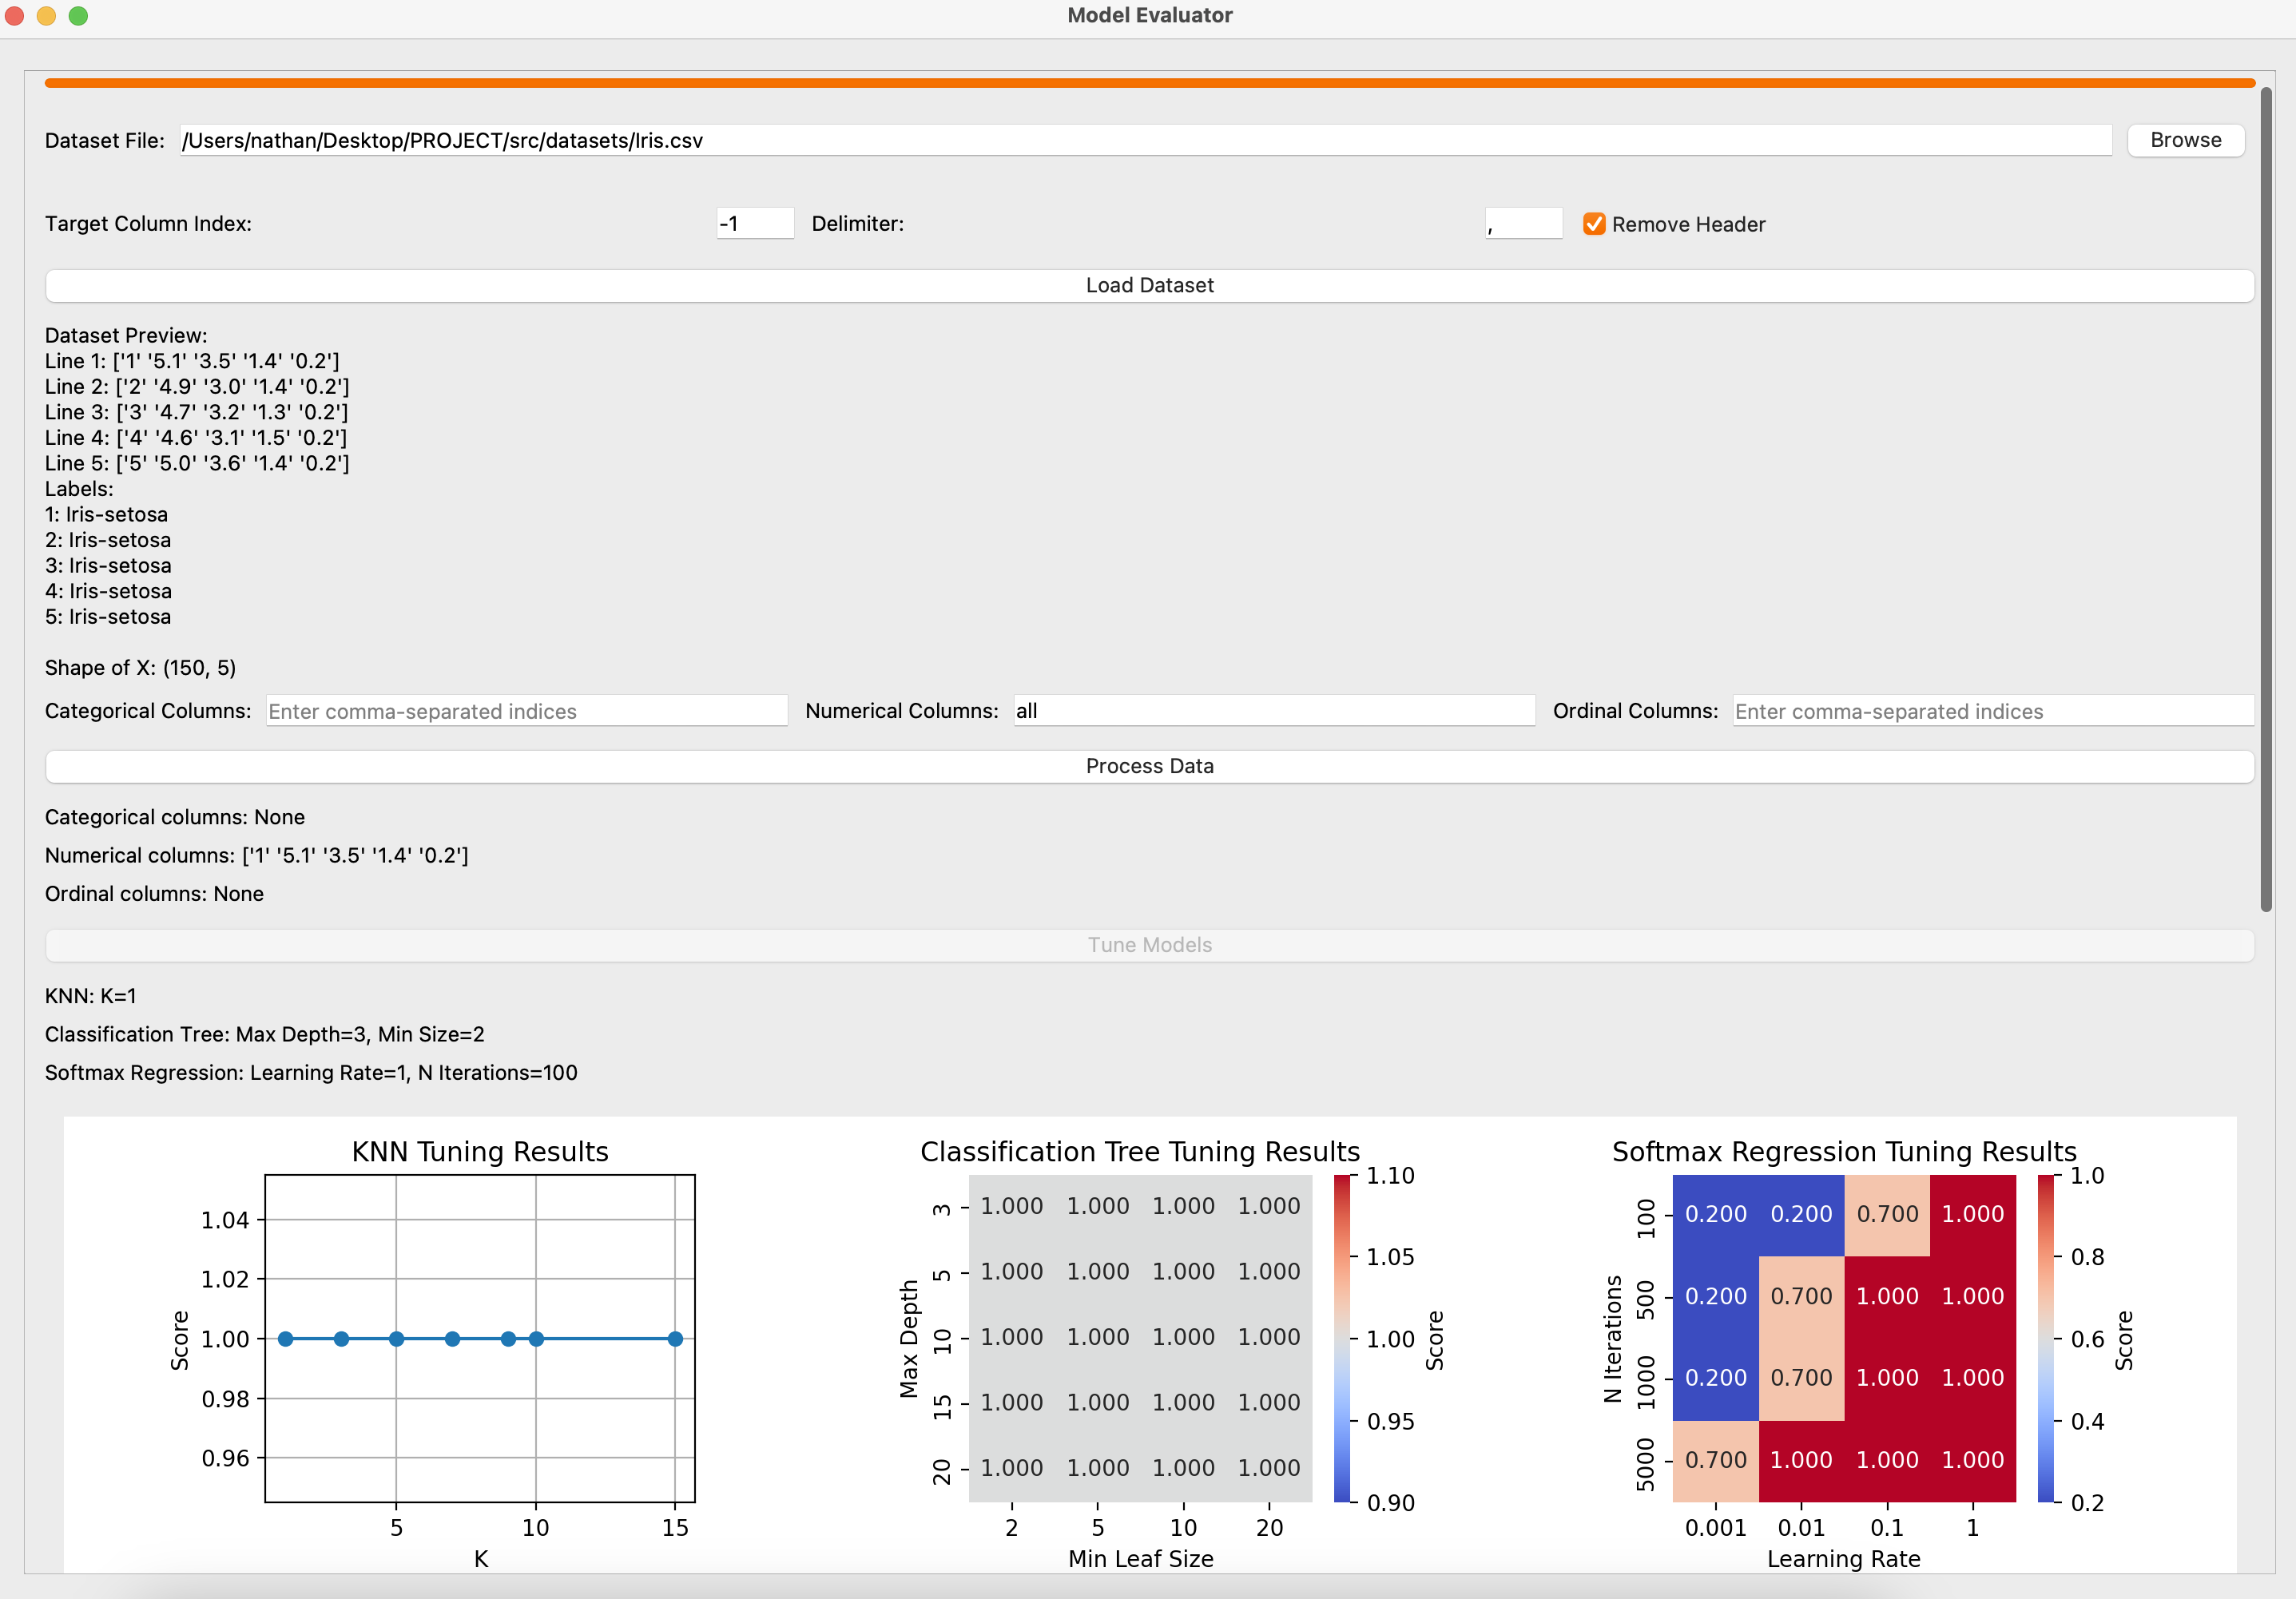
\includegraphics[width=1.0\textwidth]{app_top_preview.png}
    \caption{Top of App Interface - Loading, Preprocessing and Tuning}
    \label{fig:app_top}
\end{figure}

\begin{figure}[ht]
    \centering
    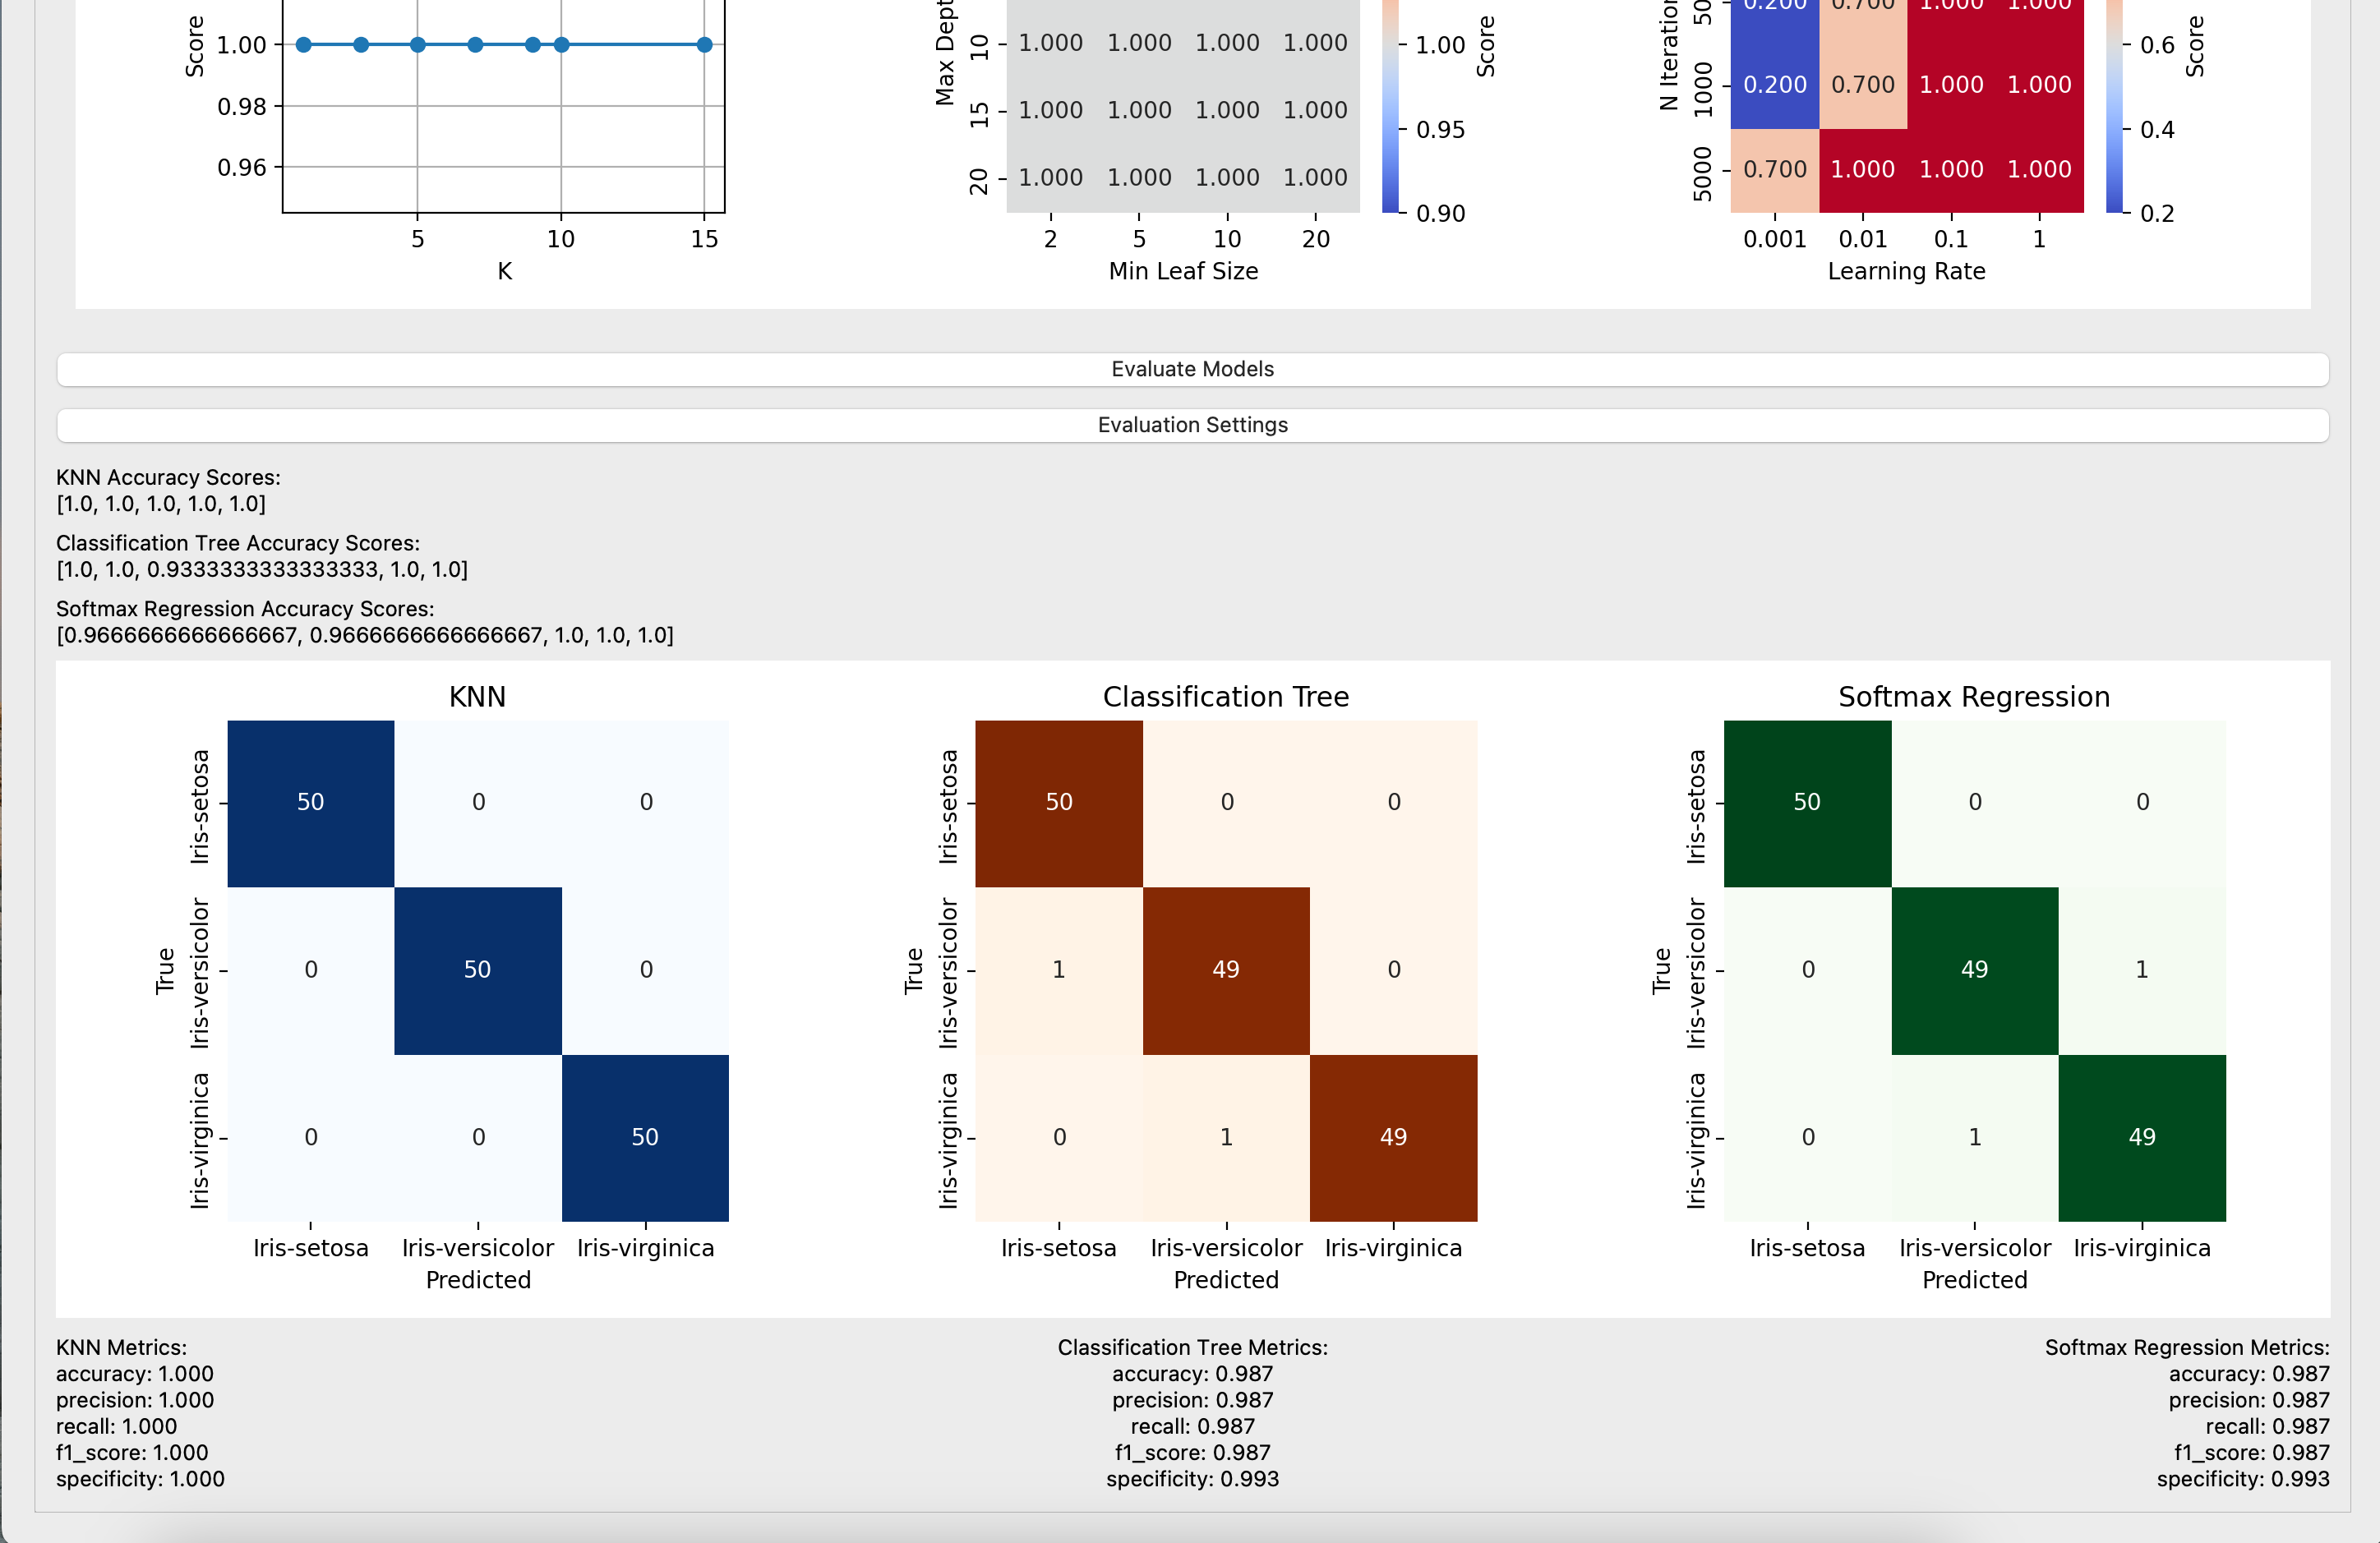
\includegraphics[width=1.0\textwidth]{app_bottom_preview.png}
    \caption{Bottom of App Interface - Model Evaluation and Results}
    \label{fig:app_bottom}
\end{figure}

\newpage
\subsection{Planning and Timescales} \label{plan}
Before we dive into my implementation, I'll bring forward the project plan put in place almost eight months ago. The timeline for Term 1 was created with a weekly outline of expected deliverables. \par
%\vspace{10mm}
\subsubsection{Term 1 Timeline}
\begin{tabular}{|c|p{10cm}|}
\hline
Timeframe & Tasks \\
\hline
Week 1 (Oct 2 - 6) & 
\makecell[l]{Focus on implementing Project Plan \\
Handwritten example of NN algorithm \\
Test out Scikit-Learn classifier functions in Jupyter Notebooks } \\
\hline
Week 2 (Oct 9 - 13) & 
\makecell[l]{1NN on simple dataset \\
Design NN data structures and UML diagrams \\
Begin PoC Programs. Fully test DTs and NN on Scikit-Learn} \\
\hline
Week 3 (Oct 16 - 20) & 
\makecell[l]{1NN on iris data, Work on multi-class data \\
Begin implementing K-Neighbours on Iris data \\
Demonstate KNN in Jupyter Notebooks, Start basic DTs} \\
\hline
Week 4 (Oct 23 - 27) & 
\makecell[l]{Complete NN Report - 29th October \\
Start working on DTs on Iris Data with binary classification \\
Begin working on hold out test set validation programs} \\
\hline
Week 5 (Oct 30 - Nov 3) & 
\makecell[l]{Start DT Report \\
Continue working on DT data handling with missing values \\
Start working on cross validation programs and test on KNN} \\
\hline
Week 6 (Nov 6 - 10) & 
\makecell[l]{Use hold out tests on Decision Trees \\
 Implement K-folds Cross Validation on both algorithms \\
Continue working on report} \\
\hline
Week 7 (Nov 13 - 17) & 
\makecell[l]{Complete DT Report - 18th November \\
Deal with any issues that have arisen over previous weeks \\
Use different datasets from UCI (e.g breast cancer)} \\
\hline
Week 8 (Nov 20 - 24) & 
\makecell[l]{ Focus on completing Interim Report \\
Amend any issues with supplementary reports if not yet finished \\
Draw meaningful tests and conclusions from results } \\
\hline
Week 9 (Nov 27 - Dec 1) & 
\makecell[l]{Work on Interim Report \\
Prepare for Demonstration and Presentation \\
Finalise project work + prepare for submission} \\
\hline
Pres. Week (Dec 4 - 8) & 
\makecell[l]{Presentation Week!\\
Submit project, and present work \\
Make demo and presentation} \\
\hline
\end{tabular}

\subsubsection{Term 2 Goals} \label{successcriteria}
Following my interim review, my third supervisor meeting and some reflection over winter break in my diary (Jan 16) - I made a list of objectives to focus on over the second term. The timeline was intentionally looser but I had a much more intuitive understanding after the first term of what needed to be achieved to complete this project:
\begin{itemize}
    \item \textbf{Preprocessing} - Handling missing and categorical data to accommodate more datasets.
    \item \textbf{Tree Refinement} - Implement optimizations to how the tree searches for splits during the training process. Alter the tree model structure so that the leaf nodes are more informative.
    \item \textbf{Metrics} - Introduce more model evaluation metrics that allow more thorough comparison and insight into the algorithms' performance.
    \item \textbf{Pipelines} - Implement pipelines that can encapsulate much of the data manipulation into few executions. This will make it easier to implement an interface for the end-user.
    \item \textbf{GUI} - Make a head start in implementing a simple but effective graphical interface for end-users to use the algorithms being discussed. Ideally, allow for inputted datasets to be analysed and trained upon.
    \item \textbf{Implement a third algorithm} given there's enough time to do so. Strongly considering logistic regression.
\end{itemize}

I'd taken lessons from the first term to adopt a looser timeframe but maintain a clear set of objectives to chase. My main priority entering second term was to implement preprocessing immediately and work from there onwards.\par
I'll address how well these plans came to fruition in the Evaluation segment, we'll now focus on the technical details of how this project came together. \par

\subsection{KNN - Start of Term 1}
\subsubsection{1-NN}
Following my Project Plan, my first step was to begin working on implementing One-Nearest Neighbours on a simple synthetic dataset. Fortunately, my lectures at Prof. Vovk's CS3920 Machine Learning course were very helpful with much of KNN's implementation - and Vovk provided a useful example in the lectures illustrating the mechanism of Nearest Neighbours in two dimensions. I took inspiration from his dataset and focused on implementing a model that could work with this 2-D coordinate data, before moving on to the Iris dataset.


\begin{lstlisting}[language=Python, caption=one\_nn.py]
    import numpy as np

class OneNearestNeighbour:
    def __init__(self):
        self.training_data = None
        self.training_labels = None

    # training of data onto labels
    def fit(self, X, y):
        self.X_training_data = X
        self.y_training_labels = y
    
    # testing function, classifies using helper method which finds euclidean distance
    def predict(self, X):
        predictions = []
        for point in X:
            predictions.append(self._predict_point(point))
        return predictions
    

    def _predict_point(self, point):
        distances = [self._euclidean_distance(point, x) for x in self.X_training_data]
        # print(distances)
        nearest = np.argmin(distances)

        return self.y_training_labels[nearest]

    def _euclidean_distance(self, p1, p2):
        return np.sqrt(np.sum((np.array(p1) - np.array(p2))**2))
\end{lstlisting}

This implementation is rather trivial. As is customary, fit() is used to train the model and predict() is used to make predictions on a test sample. The predict() method calls a helper function \_predict\_point() which predicts a label for every individual point given to it. This function calls upon the Euclidean distance function. The Euclidean Distance function basically utilises element-wise subtraction between two numpy arrays, utilising Numpy vectorization - which is generally far more efficient in practice compared to alternatives.\par 
This general structure is maintained into the KNN implementation. \par

\vspace{5pt}

I demonstrated the way this works within my first Jupyter Notebook in Figure \ref{fig:1nnjupy}. 
\begin{figure}[htbp]
    \centering
    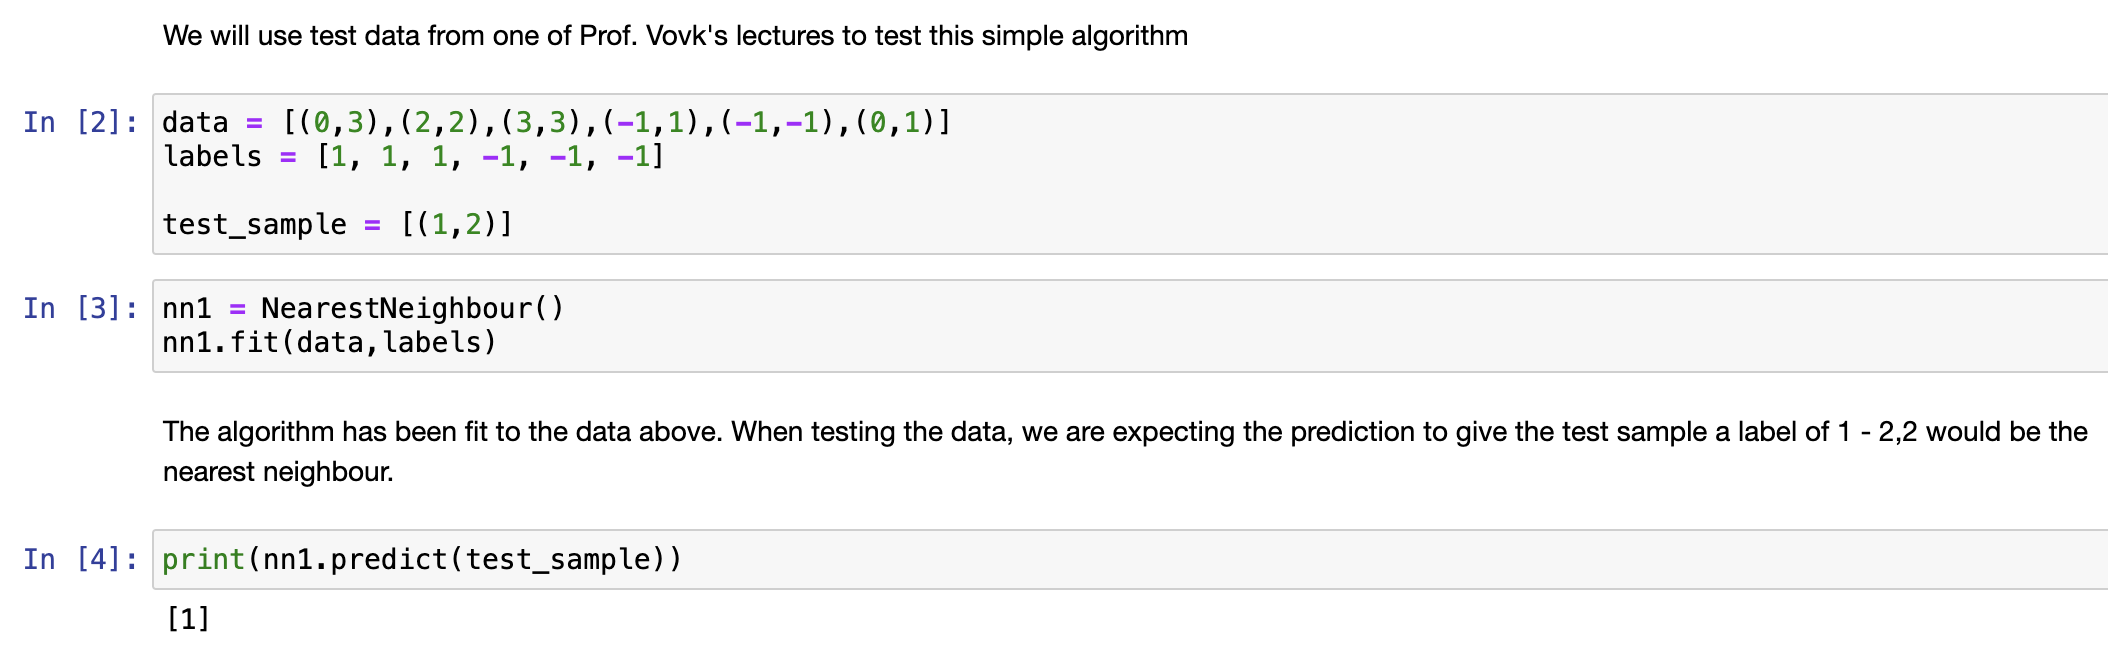
\includegraphics[width=1.25\textwidth]{1NNjupy.png}
    \caption{Notebook 1 - Fitting 1NN on simple synthetic data}
    \label{fig:1nnjupy}
\end{figure}

This notebook elaborates further on how we can also retrieve all the distances calculated and used to find the nearest neighbour for the test sample. \par

Once this was demonstrated, I focused on incorporating the iris\cite{irisdata} dataset. This also was relatively straightforward, as I essentially just utilised the load\_iris() function from the SKLearn~\cite{scikit-learn} library. This way of loading iris remains incorporated throughout the project, though other datasets are handled more manually. I could alter this later and manually add the iris dataset as a txt file using numpy\cite{numpy}. \par
It was at this point that I realised I needed to split this dataset somehow, which brings us to the next step. \par
\vspace{20pt}
\subsubsection{Train-Test-Split}
It became quickly apparent that I needed to immediately implement a way to divide the iris dataset into a training and test set, if I'm to find anything useful about my KNN implementation on the dataset. \par
Though not anticipated by my Plan, this was the next thing I decided to focus on putting together. \par

Fortunately, I found this generally to be also rather simple to implement thanks to Python's list-slicing functionality. \par
Within a train\_test\_split module that can be imported, I wanted to implement a function of the same name that took inputs \(X\) and \(y\) as features and labels respectively. The size of the test set is the key parameter, and I thought it would be useful to not only input a ratio for the test set to the training set but also a specific number of samples for the size of the test set too. \par
Over time during development, I realised during testing for edge cases that it's important to implement intensive exception handling in this function- in case an erroneous value is passed as test set size, (for example \(7.25\)). \par
It's also important that the dataset is randomly shuffled in some way, and so a complementary shuffle\_data() method is called to handle this - taking \(X\) and \(y\) as inputs with an inputted random seed value - so that we can retrieve repeatable results when we need to. \par
This overall implementation is described in Listing 2. This is the final implementation after various iterations. Some comments and PyDoc documentation have been removed for the sake of fitting this here. \par

\begin{lstlisting}[language=Python, caption=train\_test\_split.py]
def train_test_split(X, y, test_size=0.25, seed=None):  # Default test_size is now 0.25
    X = np.array(X) if not isinstance(X, np.ndarray) else X
    y = np.array(y) if not isinstance(y, np.ndarray) else y
    
    if len(X) == 0 or len(y) == 0:
        raise ValueError("Input data cannot be empty.")

    if len(X) != len(y):
        raise ValueError("The number of samples in X and y must be equal.")
    X, y = shuffle_data(X, y, seed)

    num_samples = len(y)
    
    if isinstance(test_size, float):
        if 0.0 < test_size < 1.0:
            train_ratio = num_samples - int(num_samples * test_size)
        else:
            raise ValueError("test_size as a float must be in the range (0.0, 1.0)")

    elif isinstance(test_size, int):
        if 1 <= test_size < num_samples:
            train_ratio = num_samples - test_size
        else:
            raise ValueError("test_size as an int must be less than the number of samples")

    else:
        raise ValueError("Invalid test_size value")

    X_train, X_test = X[:train_ratio], X[train_ratio:]
    y_train, y_test = y[:train_ratio], y[train_ratio:]

    return X_train, X_test, y_train, y_test

def shuffle_data(X, y, seed=None):
    rng = np.random.RandomState(seed) if seed is not None else np.random

    indices = np.arange(X.shape[0])
    rng.shuffle(indices)
\end{lstlisting}

\vspace{20pt}
At this point, it was now finally possible to train and predict our 1-Nearest Neighbour implementation on the iris dataset. This was demonstrated in the second Jupyter Notebook. \par


\begin{figure}[ht]
    \centering
    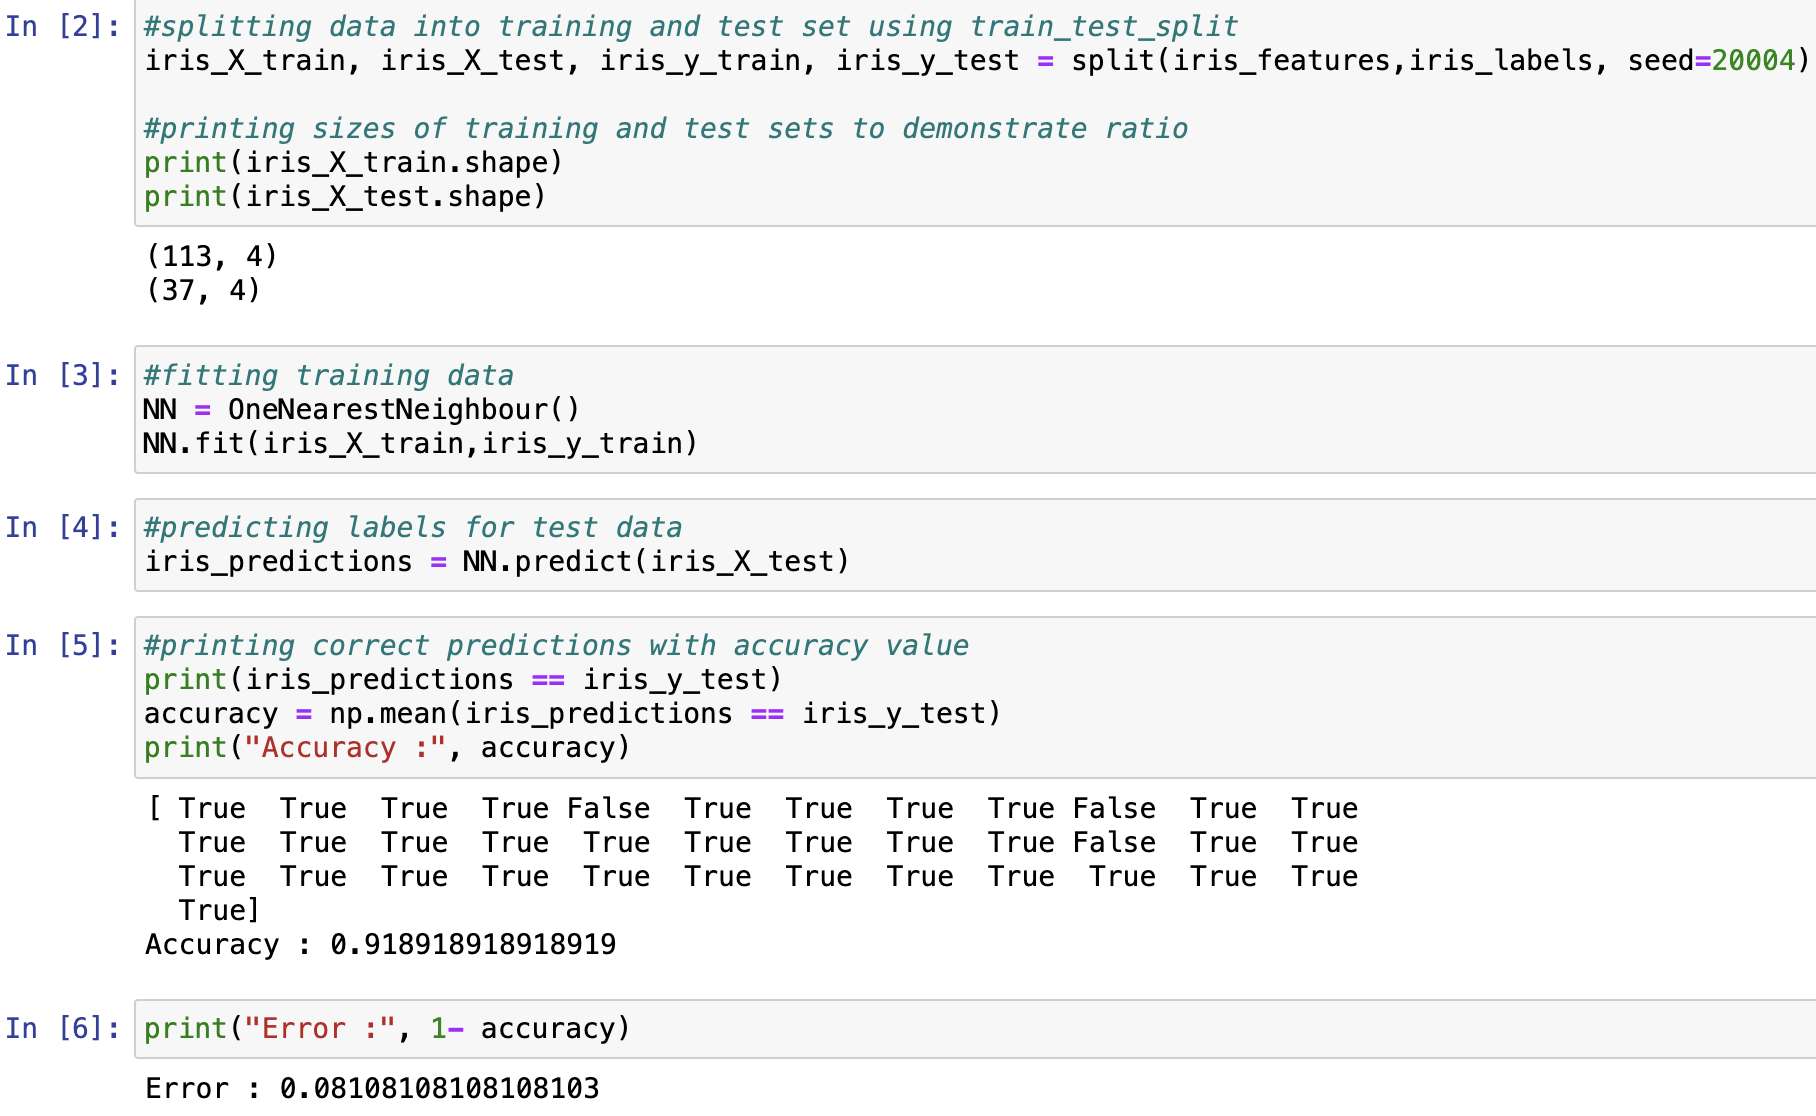
\includegraphics[width=1.25\textwidth]{1NNsplitjupy.png}
    \caption{Notebook 2 - Implementing 1NN on iris hold-out test set }
    \label{fig:1nnsplitjupy}
\end{figure}

And here we have our first evaluation of an algorithm! This was the rudimentary first step of the project, but it was a good foundation for me to work on the main K-Nearest Neighbours proof-of-concept program. Jupyter Notebooks were also my main way of demonstrating my progress in a visible way. \par

\subsubsection{Implementing K-Neighbours}
Implementing K-Nearest Neighbours followed a similar structure, but instead involved making various alterations to the way that the helper function, \_predict\_point(), works. We begin by adding an attribute, k to the constructor of the classifier - it's a parameter that we can pass to the classifier during initialisation. \par
When a point is passed from the main predict() function to the helper function, we now need to keep track of a list of points and their corresponding distances from the test point in a list. We do this with k\_nearest in the snipped shown below, where we make a list of tuples storing the index and distance, initialised as '-1' and infinity respectively. \par
We then iterate through the training set and compare each point to our test point - by iterating through our k-nearest list and replacing when we find a training point that is lower than one we've kept stored. By the end of these loops, we have a list of nearest neighbours, with their indices and distances \par
From this list, we generate a new list of tuples, containing the label of the stored point and its corresponding distance. Doing this makes it easier for us to vote for a label and handle ties if necessary \par
We then iterate through this list and count the instance of each label as well as the minimum distance found from each label compared to the test point. Finally, we use a max function to find our majority vote on the predicted label. I use a lambda function here to establish a condition such that if there's a tie in votes, we pick the closest label to the test point to predict our point. \par
I made the choice to handle ties when voting for \(K\) by simply predicting the label of the closest point - it seemed like the most intuitive way to break a tie without bringing in weighted voting - which could be implemented later but I was worried of making this calculation too inefficient. \par
\begin{lstlisting}[language=Python, caption=knn.py - \_predict\_point()]
def _predict_point(self, point):
    k_nearest = [(-1, float('inf')) for _ in range(self.k)]  # [(index, distance), ...]

        for i, training_point in enumerate(self.X_training_data):

            distance = self._euclidean_distance(point, training_point)
            
            # Check if the distance is smaller than the current k-nearest distances
            for j, (idx, dist) in enumerate(k_nearest):
                if distance < dist:
                    k_nearest.insert(j, (i, distance))
                    k_nearest = k_nearest[:self.k]  # Keep only the k-nearest distances
                    break
        # Get labels and distances of the k-nearest points
        k_labels_distances = [(self.y_training_labels[idx], dist) for idx, dist in k_nearest]

        # Count the occurrences of each label and store minimum distance for each label
        label_counts = {}
        for label, dist in k_labels_distances:
            if label not in label_counts:
                label_counts[label] = [0, float('inf')]
            label_counts[label][0] += 1  # Increase count
            label_counts[label][1] = min(label_counts[label][1], dist)  # Store the minimum distance

        # Find the label with the maximum count and if there's a tie, choose the one with the smallest distance
        majority_label = max(label_counts, key=lambda x: (label_counts[x][0], -label_counts[x][1]))

        return majority_label

\end{lstlisting}

This method is called for every point in the test set that needs to be predicted and thus the predict() method returns a list of predicted labels. \par 
At this point, we can now start using KNN on our iris data. \par

\begin{figure}[ht]
    \centering
    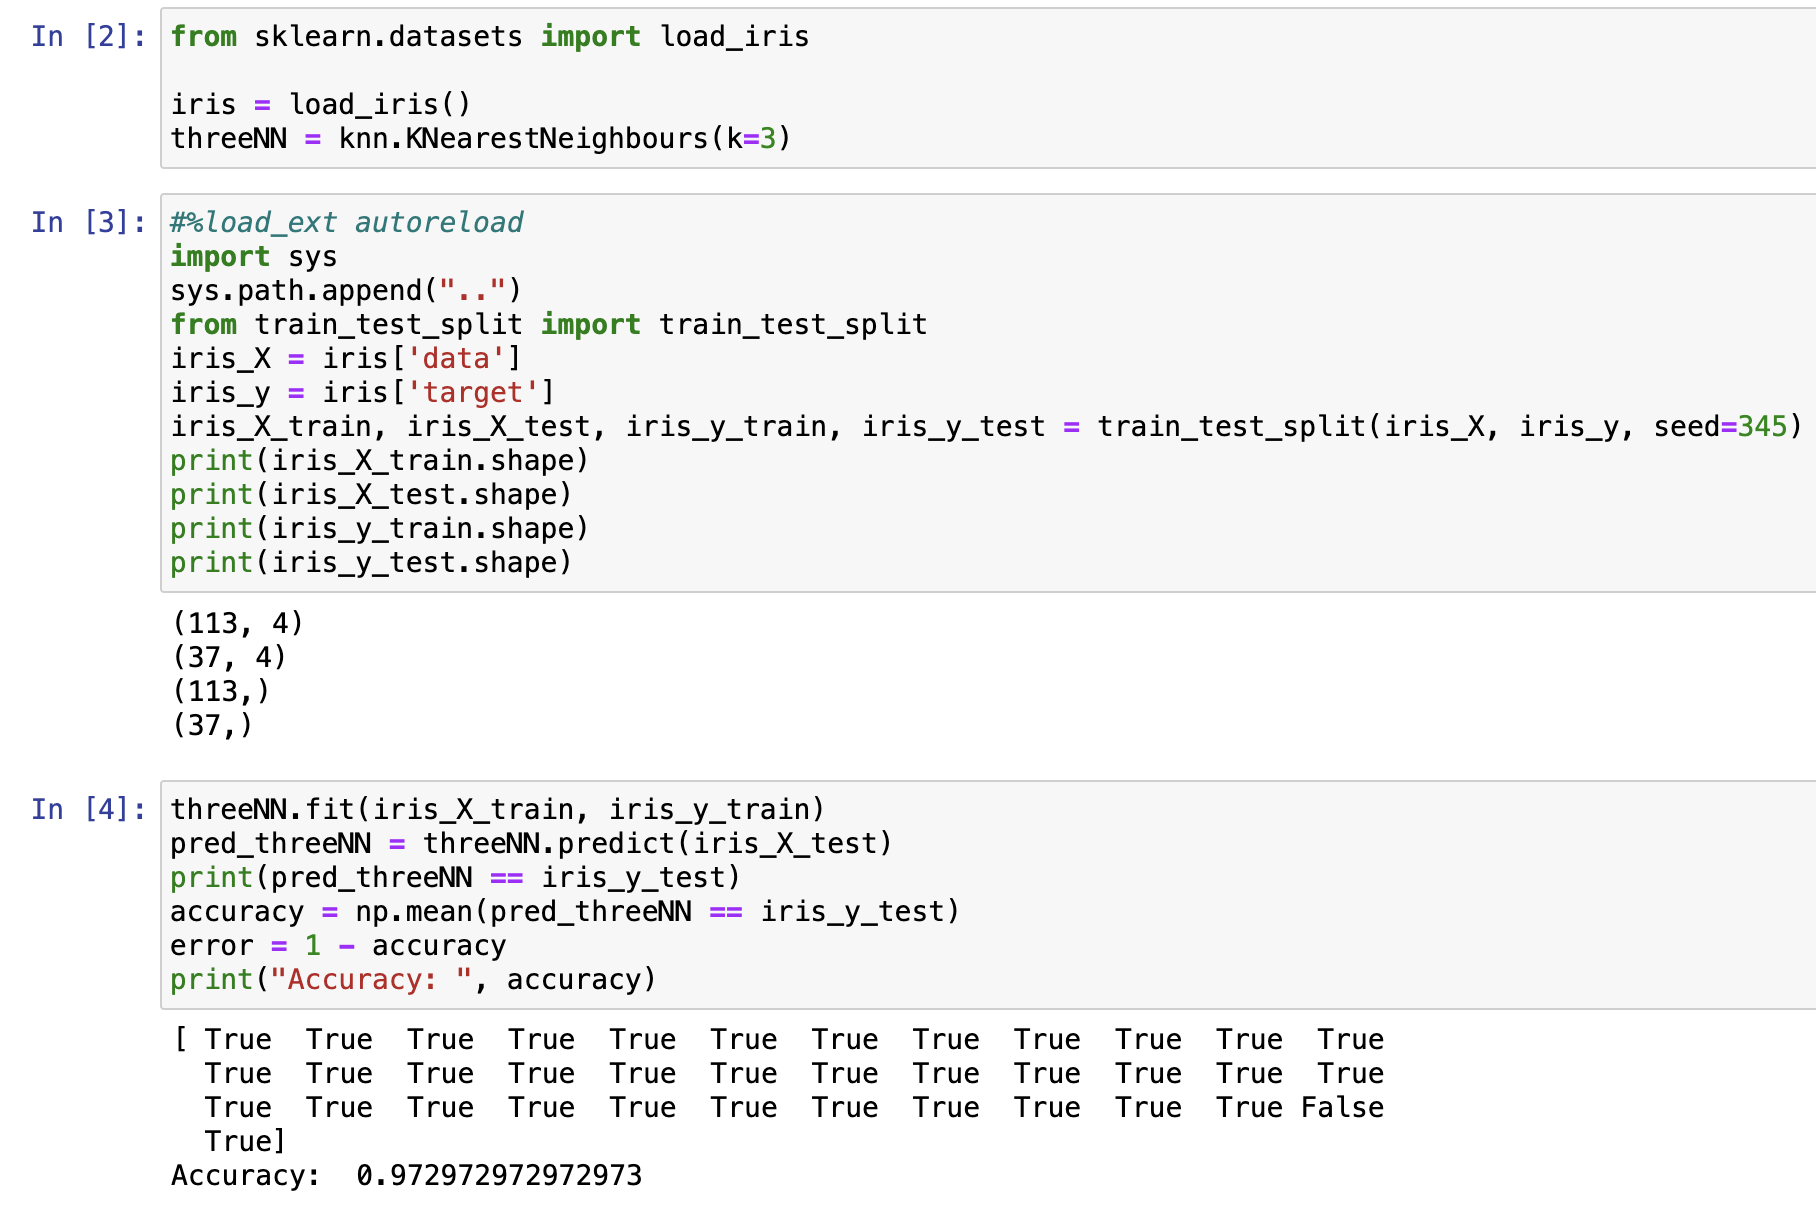
\includegraphics[width=1\textwidth]{3NNjupy.png}
    \caption{Notebook 3 - Initialising and predicting with 3 nearest neighbours}
    \label{fig:3nnjupy}
\end{figure}

In Figure \ref{fig:3nnjupy} we can see KNN getting initialised at a 3-Nearest Neighbours classifier. In code block 4, we can see the predict() function getting utilised and a list of instances of when these predictions are made correctly. \par
Within this notebook, I also investigated how the value of the hyperparameter \(K\) affected the accuracy of the KNN classifier.\par
We are essentially expecting our accuracy to decrease once the value of K becomes exceedingly high. I used a loop to iterate through various values of \(k\) and graphed the accuracies using matplotlib~\cite{matplotlib}. In Figure \ref{fig:kiris} we can see that KNN performs surprisingly well. \par
\begin{figure}[ht]
    \centering
    \begin{minipage}{0.45\textwidth}
        \centering
        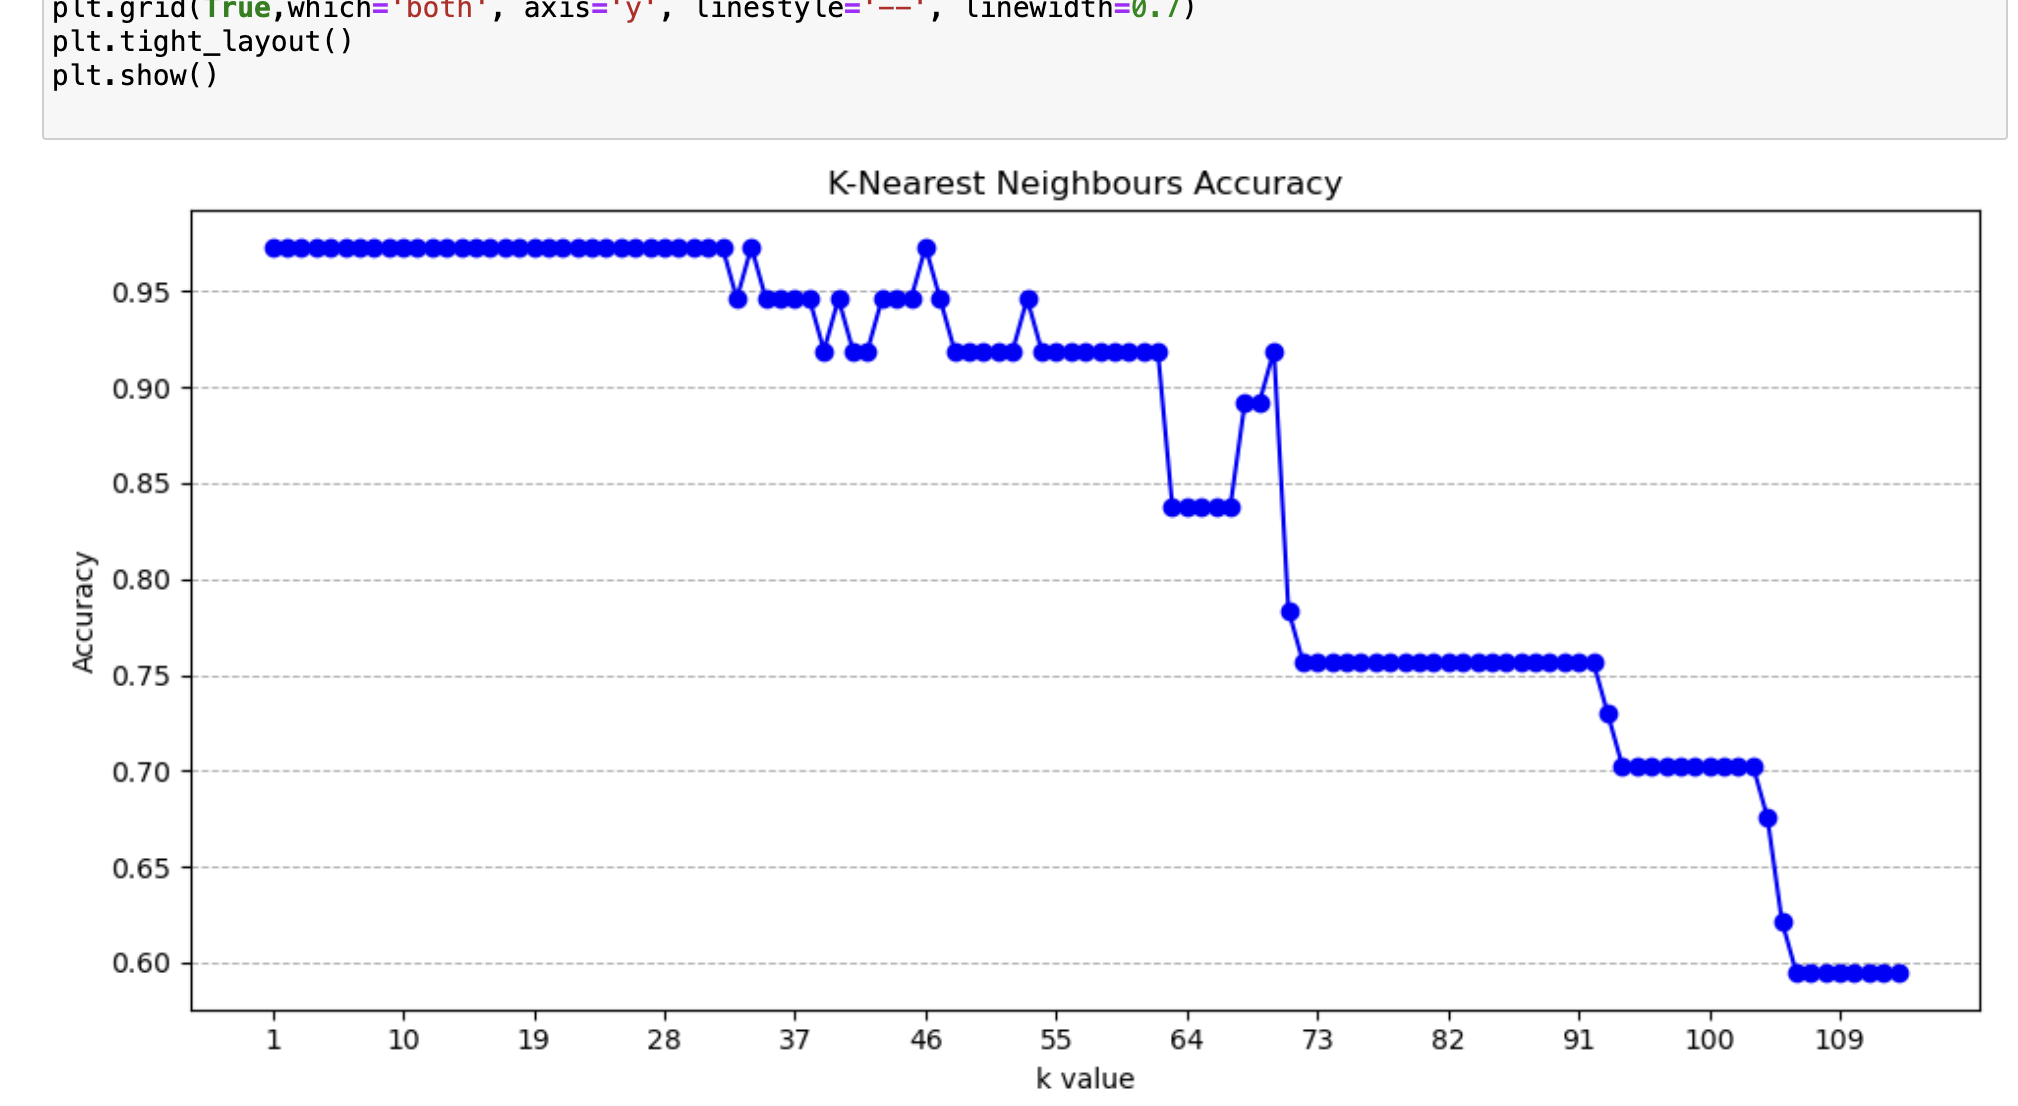
\includegraphics[width=\textwidth]{kiris.png}
        \caption{Notebook 3 - Evaluating k on iris data}
        \label{fig:kiris}
    \end{minipage}\hfill
    \begin{minipage}{0.45\textwidth}
        \centering
        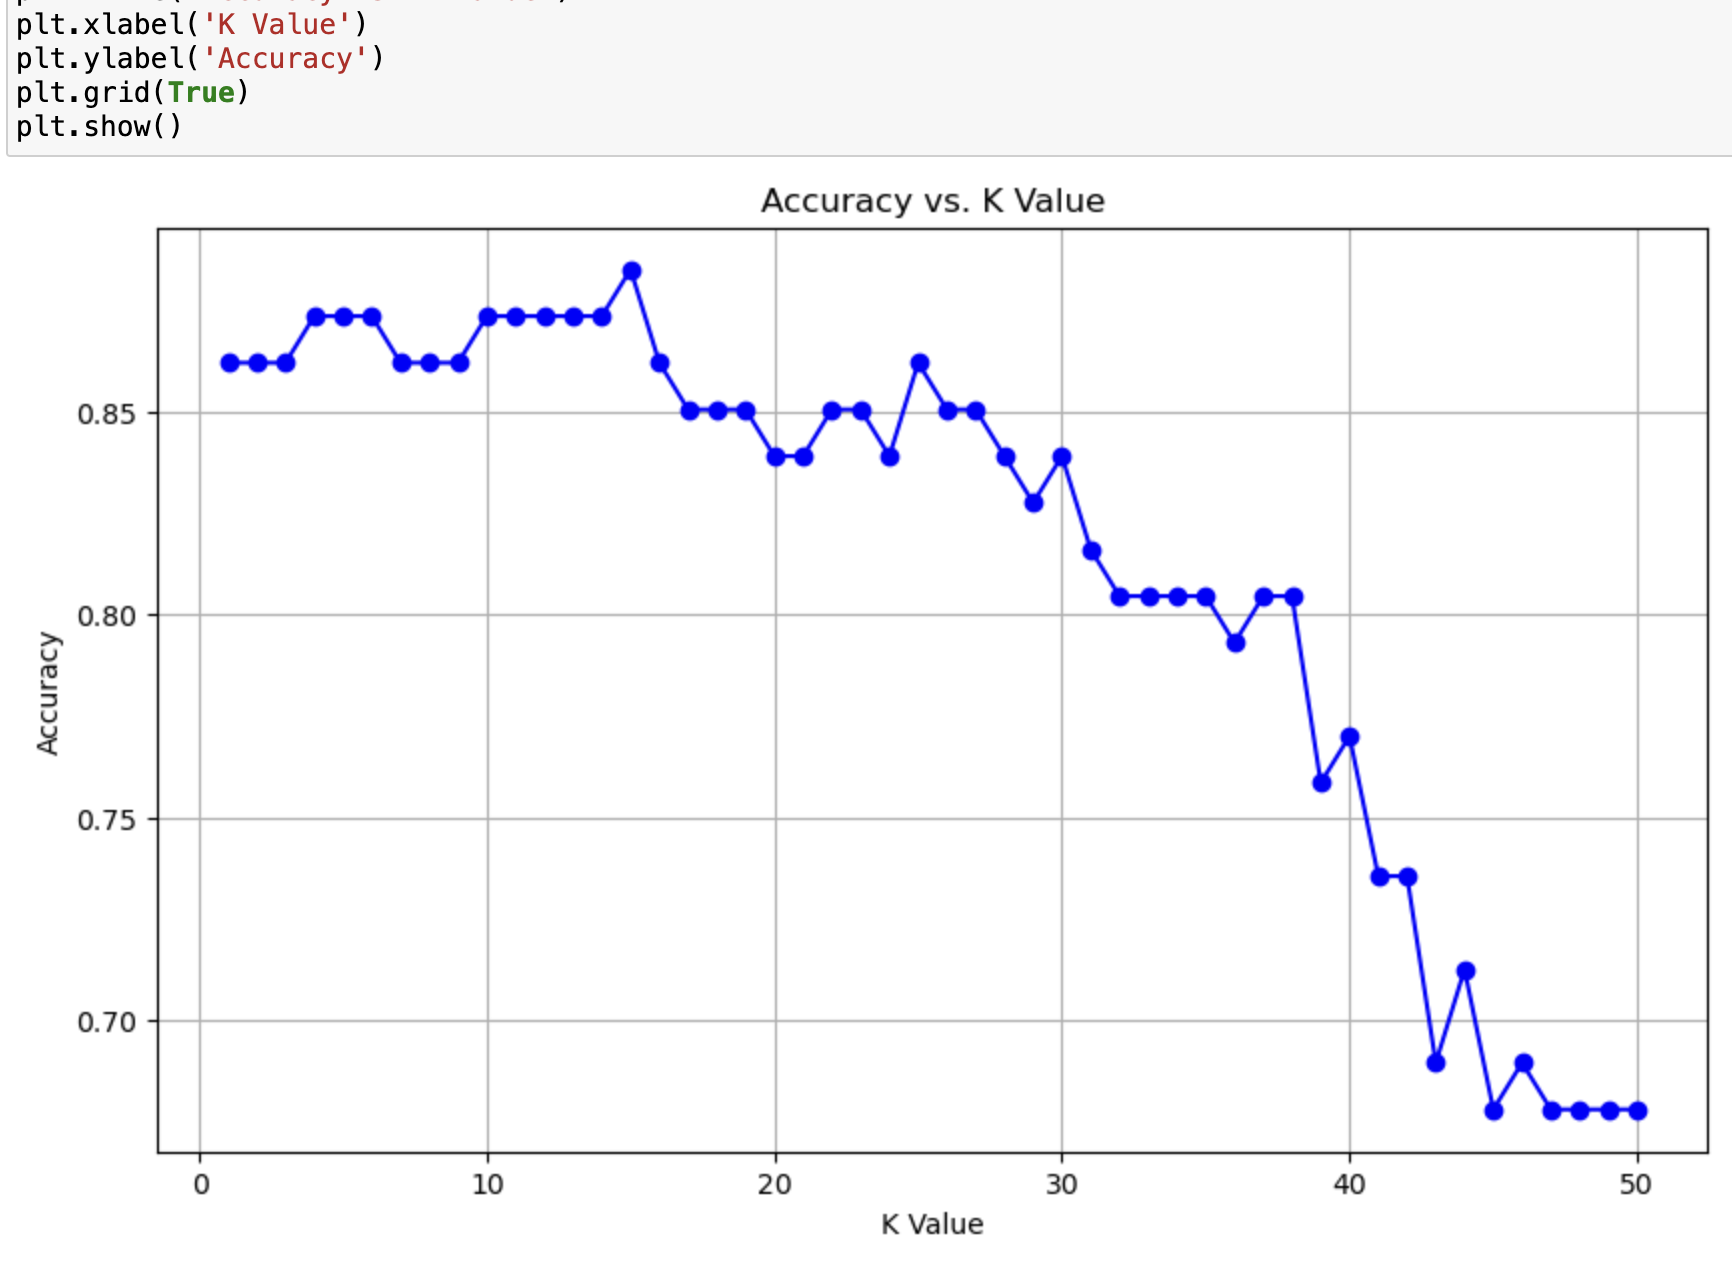
\includegraphics[width=\textwidth]{kiono.png}
        \caption{Notebook 3 - Evaluating k on ionosphere data}
        \label{fig:kiono}
    \end{minipage}
\end{figure}

I investigated this further by introducing the ionosphere~\cite{ionosphere} dataset, another UCI dataset that needs minimal preprocessing by many more features per sample. Here we can see in Figure \ref{fig:kiono} that KNN retrieves lower accuracy values in general, and the accuracy falls more sharply. Likely due to the much larger number of features in ionosphere. \par
It's at this point that I began to work on the Tree algorithm implementation.
\subsection{Classification Tree}
\subsubsection{SKLearn Implementation}
Implementing the tree algorithm was possibly the most challenging aspect of development in Term 1. I felt unfamiliar with the way that the fit() and predict() functions worked with Trees, so I utilised the SKLearn~\cite{scikit-learn} library in Notebook 4 to understand what I should expect at a higher level from my implementation. \par

\begin{figure}[ht]
    \centering
    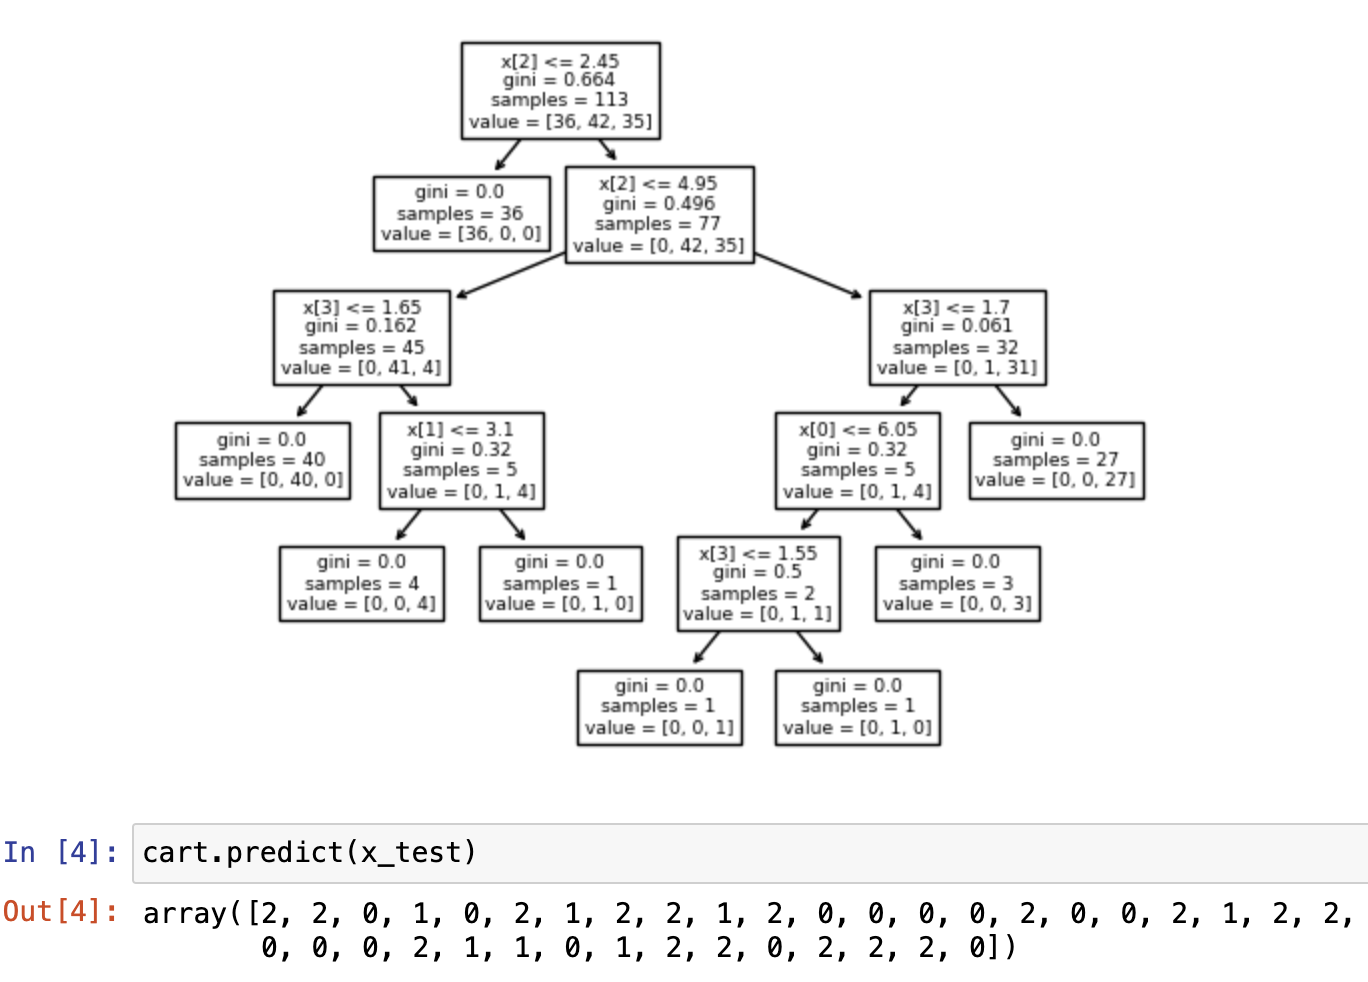
\includegraphics[width=1\textwidth]{carttree.png}
    \caption{Notebook 4 - Investigating using SKLearn}
    \label{fig:carttree}
\end{figure}

\subsubsection{Building the tree}
When fit() is called, we want our classifier to build a tree that models that training data. To do this we need to essentially, find a way to split the data continuously and recursively, such that the nodes produced are more pure than their roots. We also need to find a way to calculate this impurity and use it to traverse all the training data's features and values, to find the best thresholds that will produce this split. \par
After considering how the gini impurity should be implemented, I realised it's important to incorporate a weighted gini impurity that we can combine across both branches, so that we can aim to find a left and right branch, that have the lowest possible combined impurity. I realised that the size of both branches is something that needs to be accounted for, we want larger branches to have a greater influence if they have a low purity, as we're able to classify a larger group of samples in a split. \par

\begin{lstlisting} [language=Python, caption=classification\_tree.py - gini\_index()]
    # Gini index function to evaluate the quality of a split.
    def gini_index(self, groups, classes):
        # Count all samples at split point
        n_instances = float(sum([len(group) for group in groups]))
        # Sum weighted Gini index for each group
        gini = 0.0 # Initialize Gini index.
        for group in groups:
            size = float(len(group))
            if size == 0:  # Avoid division by zero
                continue
            score = 0.0
            # Score the group based on the score for each class
            for class_val in classes:
                p = [row[-1] for row in group].count(class_val) / size # Proportion of each class.
                score += p * p
            # Sum weighted Gini index for each group.
            gini += (1.0 - score) * (size / n_instances)
        return gini
\end{lstlisting}

Using this as a helper function, we have a way to determine the quality of our splits. \par
Looking at this at the higher level, we want our fit() function to build a tree, and we'd want a build\_tree() function to handle the split finding. I approached this in the following manner. \par

\begin{lstlisting} [language=Python, caption=classification\_tree.py - fit()]
    def fit(self, X, y):
    if len(X) == 0 or len(y) == 0:
            raise ValueError("Cannot fit a tree with an empty dataset")


        dataset = np.column_stack((X, y)).tolist()
        #print(dataset)
        self.root = self.build_tree(dataset, self.max_depth, self.min_size)
\end{lstlisting}

The fit() function combines the features and labels into a single dataset using numpy's column\_stack() functionality, and we use to\_list() to arrange this as a list of lists. What we have is, in essence, a 2-D array where each row represents a sample of features and a label at the end of the row. We now have a neat structure to manipulate within the tree. \par

\begin{lstlisting} [language=Python, caption=classification\_tree.py - build\_tree()]
    def build_tree(self, train, max_depth, min_size):
    root = self.get_split(train) # Find the best initial split for the root.
        self.split(root, max_depth, min_size, 1) # Recursively split the tree from the root node.
        # The value 1 above is passed as the first layer depth from the root
        return root
\end{lstlisting}

The tree-building function is then called by fit() and this method calls get\_split() to find the best split at this node, followed by the split() function which essentially performs this split on the tree and also assesses the stopping criteria to determine whether these nodes should continue being split, or if they can become leaf nodes - in which case the to\_terminal() method is called. \par
Within get\_split(), the test\_split() method is used to iterate through various candidate splits to help search for an ideal split. It's worth noting that this implementation is a rather greedy and inefficient algorithm, that is committed to finding the best possible split. This is something I hope to optimise to reduce training time and improve performance - by reducing overfitting. \par

\begin{lstlisting} [language=Python, caption=classification\_tree.py - get\_split()]
     # Method to find the best place to split the dataset.
    def get_split(self, dataset):
    class_values = list(set(row[-1] for row in dataset)) # Get the unique class values.
        b_index, b_value, b_score, b_groups = 999, 999, 999, None
        for index in range(len(dataset[0]) - 1): # Iterate over all features
            for row in dataset:
                groups = self.test_split(index, row[index], dataset) # Test split on each unique feature value.
                gini = self.gini_index(groups, class_values) # Calculate Gini index for the split.
                if gini < b_score: # Check if we found a better split.
                    b_index, b_value, b_score, b_groups = index, row[index], gini, groups
        return {'index': b_index, 'value': b_value, 'groups': b_groups} # Return the best split.
\end{lstlisting}

The method for finding the split is shown above. \par
Other helper methods I implemented include is\_homogenous(), which checks if the node only contains samples of the same class, and get\_depth(), which finds how deep the tree has managed to reach from the root - which mostly helped me with checking if the tree is being constructed the way I expect it to, and at what point the stopping criteria prevents the tree from reaching the maximum depth. \par
Finally, mostly to maintain an understanding of the structure and to retain my sanity, I made a print\_tree() which prints the created tree from training to the terminal. Perhaps the only implementation I've personally put together that shows a visualisation, so I'm somewhat proud of its implementation. \par

\begin{figure}[ht]
    \centering
    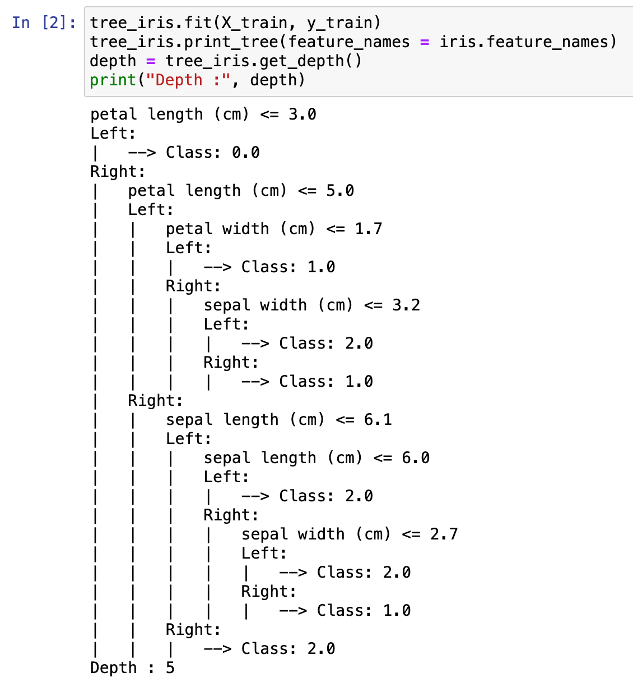
\includegraphics[width=0.5\textwidth]{printtree.png}
    \caption{print\_tree() example}
    \label{fig:printtree}
\end{figure}

\subsubsection{Making Predictions}
In theory, once we've made our tree from training - making predictions is relatively quick and straightforward. We simply take our test sample and traverse the decision nodes in the tree, until we can make our prediction at a leaf node. \par
Similar to how KNN works, we have a predict() function and a helper \_predict() function that handles each sample getting passed to it which predict iterates. \par

\begin{lstlisting} [language=Python, caption=classification\_tree.py - predict() functions]
     def predict(self, X):
        predictions = [self._predict(self.root, row) for row in X]
        return np.array(predictions)

    def _predict(self, node, row):
        if row[node['index']] < node['value']: # Check condition at the node.
            if isinstance(node['left'], dict): # If the left child is a dictionary, it's another decision node.
                return self._predict(node['left'], row)
            else:
                return node['left'] # If it's not a dictionary, it's a terminal node.
        else:
            if isinstance(node['right'], dict):
                return self._predict(node['right'], row)
            else:
                return node['right']
\end{lstlisting}

\subsection{Cross-Validation}
\subsubsection{Retrieving K-Folds}
Once both algorithms has been implemented, I wanted to Implement K-folds Cross-Validation immediately to properly evaluate and compare these two algorithms at how well they made predictions. Approaching this wasn't too difficult compared to the Tree, and the fold-making aspect essentially had a lot of similarities with the train-test-split implementation, with more iterations. \par
I approached this by making a function, \_k\_folds(), that separates the set given into the number of folds given. This essentially returns a list of folds, comprised of training and test data for features and labels - so four lists of data within each 'fold' of the folds lists. \par

\begin{lstlisting} [language=Python, caption=cross\_validation.py - \_k\_folds()]
     def _k_folds(X, y, k=5, seed=None) :
      X, y = split.shuffle_data(X,y,seed)
    num_of_samples = len(y)
    # Check if 'k' is a valid value
    #K can't be 1, we accept 2 and higher
    if k < 2 or k > num_of_samples or not isinstance(k, int):
        raise ValueError(f"'k' must be an integer between 2 and {num_of_samples}, got {k}")
    indices = np.arange(num_of_samples)

    # Calculate the standard fold size
    fold_size = num_of_samples // k
    remainder = num_of_samples % k
    #unused but may be useful if we optimise remainder-handling

    # Initialize an array to store the training and testing sets for each fold
    folds = []

    current = 0
    for i in range(k):
        if i < k - 1:
            start, stop = current, current + fold_size
        else:
            # For the last fold, use the remaining samples
            start, stop = current, num_of_samples

        test_indices = indices[start:stop]
        train_indices = np.concatenate([indices[:start], indices[stop:]])

        X_train, X_test = X[train_indices], X[test_indices]
        y_train, y_test = y[train_indices], y[test_indices]

        folds.append(((X_train, y_train), (X_test, y_test)))

        current = stop

    return folds
\end{lstlisting}
I realised that there are various ways to approach the problem regarding the remainder of samples that don't evenly fit into the division of folds - my implementation simply allowed the final fold to handle the remainder, so this fold could be larger or smaller in comparison to the rest. This could be optimised a little, such that the remainder is evenly distributed across all the folds, but for now I chose the simpler approach. The caveat is if a significantly large number of folds is requested (say where \(k > (n/2)\)), the final fold will be quite unusually sized in comparison to the rest. But this is an unusual situation to be in anyway. \par

\subsubsection{Calculating the scores}
I decided, for simplicity, to allow a function to take the model, the features and labels, and the number of folds with a shuffle seed - all as parameters. And the function will perform all the training and testing using the model's defined fit() and predict() functions and retrieve a list of accuracy scores to be interpreted. 

\begin{lstlisting} [language=Python, caption=cross\_validation.py - accuracy scores]
     def k_folds_accuracy_scores(model, X, y, k=5, seed=None):
      # Check if the model has 'fit' and 'predict' methods
    if not hasattr(model, 'fit') or not callable(getattr(model, 'fit')):
        raise AttributeError("The provided model does not have a callable 'fit' method.")
    if not hasattr(model, 'predict') or not callable(getattr(model, 'predict')):
        raise AttributeError("The provided model does not have a callable 'predict' method.")


    # Generate folds using the previously defined k_folds function
    folds = _k_folds(X, y, k, seed)

    # List to store the scores from each fold
    scores = []

    # Iterate over each fold
    #n=0
    #mismatch = 0
    for (X_train, y_train), (X_test, y_test) in folds:
        # Fit the model on the training set
        model.fit(X_train, y_train)

        # Predict on the test set
        y_pred = model.predict(X_test)

        # Compute the score - here, we use accuracy as an example
        accuracy = np.mean(y_pred == y_test)


        # Append the score to the list
        scores.append(accuracy)
       

    return scores
      
\end{lstlisting}
This was an exciting thing to put together, as it would essentially be the first time all these abstractions I've made can finally fit together in one function. Implementation here was relatively simple, but it was important that exception handling here was robust, as we're assuming that the models in place have the functions we need to retrieve these performance scores.  \par
Once this was implemented, it was natural to make more functions that retrieves the mean of these scores, and also perform LOOCV. Implementing these was trivial, as it essentially just called the function above. \par

\subsection{MinMaxScaler - End of Term 1}
Data preprocessing hasn't been covered a lot in this report but it's significance became far more apparent to me rather late in the first term, when I realised there's many factors preventing me from using these algorithms on more interesting datasets. My supervisor also emphasised the importance of normalising data that will be trained by KNN, as KNN is scale-sensitive. \par
Due to this, I very quickly implemented a MinMaxScaler - which essentially fits all data passed to it on a scale from 0 to 1. The scaler is in the form of a class, which means that it can be fitted in accordance to a particular training set, and then apply that same transformation to a test set, as is necessary for a scaler in ML settings. \par


\begin{lstlisting} [language=Python, caption=preprocessing.py - MinMaxScaler]
import numpy as np

class MinMaxScaler:
    def __init__(self):
        self.min_ = None
        self.max_ = None
        self.range_ = None

    def fit(self, X):
        """Fit the scaler to the data."""
        self.min_ = np.min(X, axis=0)
        self.max_ = np.max(X, axis=0)
        self.range_ = self.max_ - self.min_
        # Handle zero range to avoid division by zero
        self.range_[self.range_ == 0] = 1
        return self
        

    def transform(self, X):
        """Transform the data using the fitted scaler."""
        if self.min_ is None or self.max_ is None:
            raise RuntimeError("The scaler has not been fitted yet.")
        return (X - self.min_) / self.range_

    def fit_transform(self, X):
        """Fit to data, then transform it."""
        return self.fit(X).transform(X)
      
\end{lstlisting}

This module will come useful in future implementations, I see this class as the first of various other functions in this module, with handling categorical data and missing data. \par

\subsection{Preprocessing - Start of Term 2}
Following an interim review with favourable feedback, I pushed onwards and made a set of goals as mentioned in the Timescales section. My biggest bother in December is that my algorithms were constrained only to numerical data, so my main priority was to implement this immediately. \par
\subsubsection{Sci-Kit Learn Examples}
Some quick research introduced me to the use of Encoders in SKLearn. I began development by making a new Jupyter notebook and experimenting with existing examples on Notebook 7. \par

\begin{figure}[ht]
    \centering
    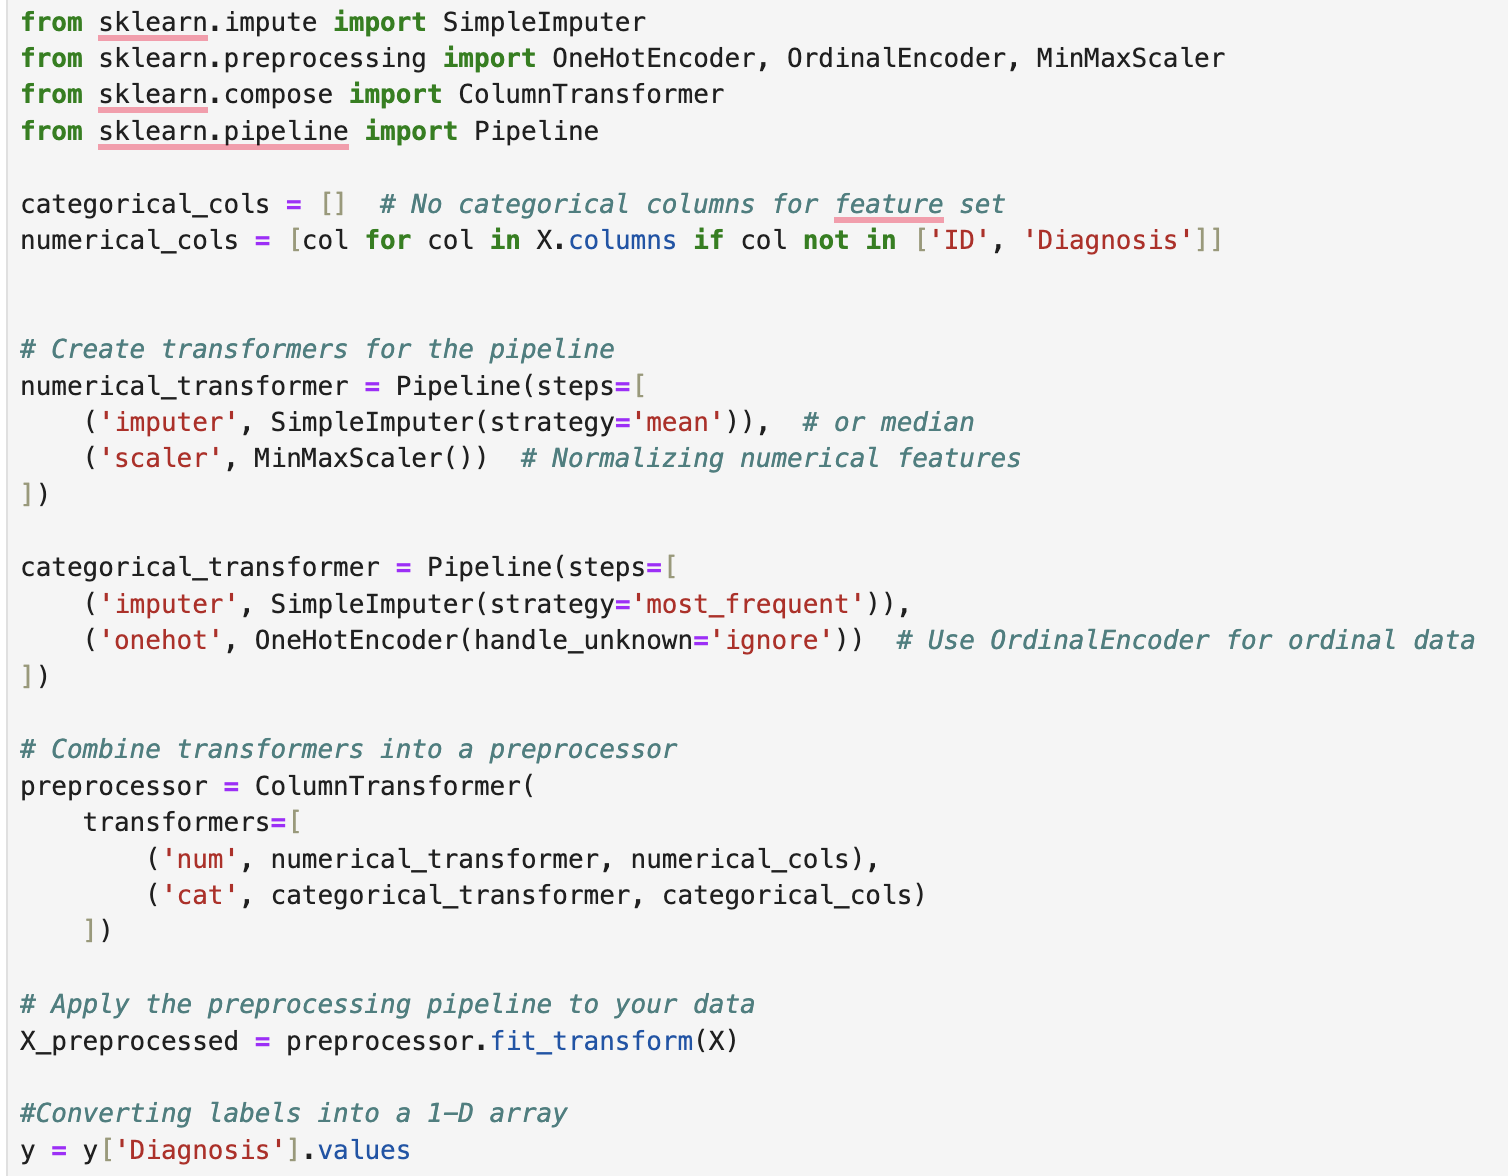
\includegraphics[width=0.8\textwidth]{notebook_7_1.png}
    \caption{Working with SKLearn Preprocessing Tools on the Breast Cancer Dataset - Notebook 7}
    \label{fig:notebook_7_1}
\end{figure}

The UCI Wisconsin Breast Cancer dataset~\cite{breastcancerdataset_wisconsion} was a dataset I wanted to work with in the previous term but couldn't due to a lack of preprocessing on my end. It was during this process that I learned that each of these preprocessing tools work as components of a larger sequential pipeline, and these pipelines can be arranged depending on the type of data - ordinal, categorical and numerical. I also found use with the ColumnTransformer to combine preprocessing pipelines into a single unit. \par
I had a greater sense of what I needed to implement, and how preprocessing is a quite a lot more complicated than expected. \par
This notebook was quite insightful for me as it allowed me to also evaluate how well the models I'd created were able to perform on datasets that I'd not been able to work with prior. It was reassuring to see that my models continued to work as expected, once data was transformed appropriately. Notebook 7 continues and covers training on 4 datasets that were otherwise out of reach for use. Another dataset explored here was the Car Evaluation dataset, which uses entirely categorial/ordinal data.  \par

\subsubsection{Preprocessing Module}

With the tools from Notebook 7 kept in mind, I began developing my own in a file named preprocessing.py. This file becomes my main preprocessing module that is used for all data handling in the app. \par

My initial goals we to implement the following, handling missing data and categorical datasets. It became apparent to me that it's important to use separate encoders for categorical and ordinal data (categorised data that have an inherent order in value, like high, medium, low). \par 
\begin{itemize}
\item \textbf{MinMaxScaler:} A scaler that scales features to a specified range, typically between 0 and 1, to ensure that all features contribute equally to the model.

\item \textbf{SimpleImputer:} A transformer that imputes missing values in the dataset using various strategies such as mean, median, most frequent, or a constant value.

\item \textbf{OneHotEncoder:} A transformer that converts categorical features into a binary vector representation, creating a new binary feature for each unique category.

\item \textbf{OrdinalEncoder:} A transformer that encodes categorical features with an ordinal relationship, preserving the order of the categories while converting them to numerical values.


\end{itemize}

SimpleImputer was probably the most challenging to implement, as it had to handle all kinds of possible data. I also wanted to provide many possible strategies depending on what the user and the dataset needed. \par
It may be worth noting that this is one of the very few occasions that pandas is utilised to handle any discrepancies, I otherwise stuck to NumPy as often as I could. \par

\begin{lstlisting} [language=Python, caption=preprocessing.py - SimpleImputer - fit()]
def transform(self, X):
    if isinstance(X, pd.DataFrame):
                # Convert DataFrame to numpy array
                X = X.values
    
            self.statistics_ = []
            for column in X.T:
                try:
                    # Attempt to convert the column to float, ignoring empty spaces
                    column_float = np.array([float(x) if x.strip() else np.nan for x in column])
                    # Handle numeric columns
                    if self.strategy == 'mean':
                        self.statistics_.append(np.nanmean(column_float))
                    elif self.strategy == 'median':
                        self.statistics_.append(np.nanmedian(column_float))
                    elif self.strategy == 'most_frequent':
                        self.statistics_.append(np.nanmax(np.bincount(column_float[~np.isnan(column_float)].astype(int))))
                    elif self.strategy == 'constant':
                        self.statistics_.append(self.fill_value)
                    else:
                        raise ValueError(f"Strategy '{self.strategy}' not supported for numeric data")
                except ValueError:
                    # Handle non-numeric columns
                    if self.strategy == 'most_frequent':
                        most_common = Counter(column[column != '']).most_common(1)
                        self.statistics_.append(most_common[0][0] if most_common else self.fill_value)
                    elif self.strategy == 'constant':
                        self.statistics_.append(self.fill_value)
                    else:
                        raise ValueError(f"Strategy '{self.strategy}' not supported for non-numeric data")
    
            self.statistics_ = np.array(self.statistics_)
            return self

\end{lstlisting}

Each of these classes utilise the typical fit() and transform() functions that you'd usually find in these preprocessing utilities. The fit method is called on the training data to learn the necessary parameters or statistics from the data, while the transform method applies the learned transformations to the data. The fit\_transform method combines both steps, fitting the transformer on the training data and immediately applying the transformation. \par

\subsubsection{Combining into Pipelines}
As seen in Notebook 7, these classes become far more powerful when they're combined into pipelines or even a combination of pipelines. Not only is this easier to work with, but vitally - it makes it far easier to implement an entire preprocessing workflow behind-the-scenes of a GUI interface. The goal is to create something like a single CombinedPrepreprocessor that can handle all aspects of the data preprocessing tasks with three built-in preprocessing pipelines, for numeric, categorical and ordinal data accordingly. Creating this abstraction allows an entire preprocessing workflow to be passed with a dataset and model as a parameter. It was vital for me to implement this to start working on the GUI later on. \par
The CombinedPreprocessor essentially takes a dictionary of pipelines upon initialisation. It was important that this was made flexible during occasions when the dataset only used one type of data. I realised this later in development when my CombinedPreprocessor expected three pipelines when the dataset really only needed one. \par
Along with the pipeline class and the combined prepreprocessor class, I also implemented a LabelEncoder - which I realised was rather important for my y-labels in my dataset. I almost forgot that labels need preprocessing as well as the the features! Some of my implementations needed this in order to make suitable predictions, and the mapping within the encoder was useful when displaying results. \par
I found that building a numeric converter was also useful in certain cases depending on the dataset being used. \par
All in all, these were the additional classes defined in the preprocessing module. \par
\begin{itemize}


\item \textbf{PreprocessingPipeline:} A pipeline that applies a sequence of transformers to the data in a specified order, allowing for a streamlined preprocessing workflow.

\item \textbf{LabelEncoder:} A transformer that encodes labels as integers, mapping each unique label to a corresponding integer value.

\item \textbf{NumericConverter:} A converter that transforms non-numeric data to numeric, handling cases where the data cannot be directly converted to float.

\item \textbf{CombinedPreprocessor:} A preprocessor that combines multiple preprocessing pipelines for different subsets of features, allowing for customized preprocessing based on the characteristics of each feature subset.

\end{itemize}
\begin{lstlisting} [language=Python, caption=preprocessing.py - PreprocessingPipeline] 
class PreprocessingPipeline:
    def __init__(self, steps: List[Tuple[str, object]]):
        self.steps = steps
        self._validate_steps()
        self.fitted_ = False

    def _validate_steps(self):
        required_methods = ['fit', 'transform']
        for name, transformer in self.steps:
            if not isinstance(name, str):
                raise ValueError(f"Step name '{name}' is not a string.")
            if not all(hasattr(transformer, method) for method in required_methods):
                missing_methods = [method for method in required_methods if not hasattr(transformer, method)]
                raise TypeError(f"Transformer '{type(transformer).__name__}' is missing required methods: {', '.join(missing_methods)}.")

    def fit(self, X, y=None):
        for _, transformer in self.steps:
            if hasattr(transformer, 'fit_transform'):
                X = transformer.fit_transform(X)
            else:
                transformer.fit(X, y)
                X = transformer.transform(X)
        self.fitted_ = True
        return self

    def transform(self, X):
        if not self.fitted_:
            raise RuntimeError("The pipeline has not been fitted yet. Call 'fit' before 'transform'.")
        for _, transformer in self.steps:
            X = transformer.transform(X)
        return X

    def fit_transform(self, X, y=None):
        return self.fit(X, y).transform(X)

\end{lstlisting}

\begin{lstlisting} [language=Python, caption=preprocessing.py - CombinedPreprocessor] 
class CombinedPreprocessor:

    def __init__(self, **pipelines):
        self.pipelines = pipelines

    def fit(self, X, y=None):
        for pipeline_name, (pipeline, columns) in self.pipelines.items():
            if len(columns) == 0:
                continue  # Skip the pipeline if there are no corresponding columns
            try:
                if columns is not None:
                    X_subset = X[:, columns]
                    pipeline.fit(X_subset)
                else:
                    pipeline.fit(X)
            except ValueError as e:
                raise ValueError(f"Error fitting {pipeline_name} pipeline: {str(e)}")
        return self

    def transform(self, X):
        transformed_subsets = []
        for pipeline_name, (pipeline, columns) in self.pipelines.items():
            if len(columns) == 0:
                continue  # Skip the pipeline if there are no corresponding columns
            try:
                if columns is not None:
                    X_subset = X[:, columns]
                    if hasattr(pipeline, 'transform'):
                        transformed_subset = pipeline.transform(X_subset)
                    else:
                        transformed_subset = X_subset  # Use original subset if pipeline has no transform method
                else:
                    if hasattr(pipeline, 'transform'):
                        transformed_subset = pipeline.transform(X)
                    else:
                        transformed_subset = X  # Use original data if pipeline has no transform method
                transformed_subsets.append(transformed_subset)
            except ValueError as e:
                raise ValueError(f"Error transforming {pipeline_name} pipeline: {str(e)}")
        try:
            X_transformed = np.hstack(transformed_subsets)
            return X_transformed
        except ValueError as e:
            raise ValueError(f"Error stacking transformed subsets: {str(e)}")

    def fit_transform(self, X, y=None):
        self.fit(X, y)
        return self.transform(X)


\end{lstlisting}
\subsubsection{Loading From A File}\label{fileloading}

There's one more function in this module, with a vital but slightly different task. I wanted to make a function that could handle any inputted file and turn it into X, a set of features, and y, a set of target values. This obviously required much tinkering with, as we need to know from our user where the target column is in our dataset (i.e. which column in our table of values corresponds to the y-target labels). \par
This is quite a vital utility in my application, as this is the function that is called every time a file is inputted into the application. I needed to make this function flexible and constrained in the right places, and it involved getting quite familiar with csv and numpy's libraries and capabilities. \par
One challenge is that quite a few datasets are tab-delimited. This means that rather than using a comma or semi-colon to separate each feature in the dataset - quite a nuisance but many interesting datasets online are arranged in this way. I used Python's native open() function for these situations and my application follows a protocol such that if the user inputs "\textbackslash t" in the delimiter input space, the file reader will anticipate this when loading the file. Essentially, my app expects a ",", ";" or "\textbackslash t" as a possible delimiter. \par
The function has a few more capabilities, like allowing the user to give a heads-up of what the datatype is, and if a header row is in the dataset. The header row functionality is simple but important, many datasets include a header row that, if included in the dataset during loading, will throw many data type errors during preprocessing. This has translated to the checkbox seen in the GUI. \par

\begin{itemize}
 
\item \textbf{{load\_dataset}:} A utility function that loads a dataset from a file and splits it into features (X) and target (y) using NumPy, handling various file formats, missing values, and target column specification.

\end{itemize}

\begin{lstlisting} [language=Python, caption=preprocessing.py - load\_dataset()] 
def load_dataset(file_path, target_col=-1, sep=',', missing_values=None, drop_missing=False, dtype=None, header=False):
    try:
        data = []
        with open(file_path, 'r') as file:
            if sep == '\t' :
                for line in file:
                    row = line.strip().split()
                    data.append(row)
            else:
                csv_reader = csv.reader(file, delimiter=sep)
                if header:
                    next(csv_reader)  # Skip the header row
                for row in csv_reader:
                    data.append([value.strip() for value in row])

        data = np.array(data, dtype=dtype)

        # Handle missing values
        if missing_values:
            mask = np.isin(data, missing_values)
            data[mask] = np.nan
        if drop_missing:
            data = data[~np.isnan(data).any(axis=1)]

        # Extract the features (X) and target (y)
        if target_col < 0:
            target_col = data.shape[1] + target_col
        if 0 <= target_col < data.shape[1]:
            if target_col == data.shape[1] - 1:
                X = data[:, :-1]
            else:
                X = np.concatenate((data[:, :target_col], data[:, target_col+1:]), axis=1)
            y = data[:, target_col]
        else:
            raise ValueError(f"Invalid target column index: {target_col}")

        return X, y

    except FileNotFoundError:
        raise FileNotFoundError(f"File not found: {file_path}")
    except IOError as e:
        raise IOError(f"An error occurred while reading the file: {e}")
    except ValueError as ve:
        raise ValueError(f"Invalid file format or target column: {ve}")
    except Exception as e:
        raise Exception(f"An error occurred while loading the dataset: {e}")

\end{lstlisting}

\subsubsection{Putting It Together}
There's a lot of moving pieces in this module, but implementing this module allowed me to use my models on virtually any dataset I was able to find online. \par
I showcase all of this functionality in Notebook 9 (at which point, I also had Softmax Regression ready to use too). This notebook demonstrates rather succinctly everything discussed that's been implemented. \par

\begin{figure}[ht]
    \centering
    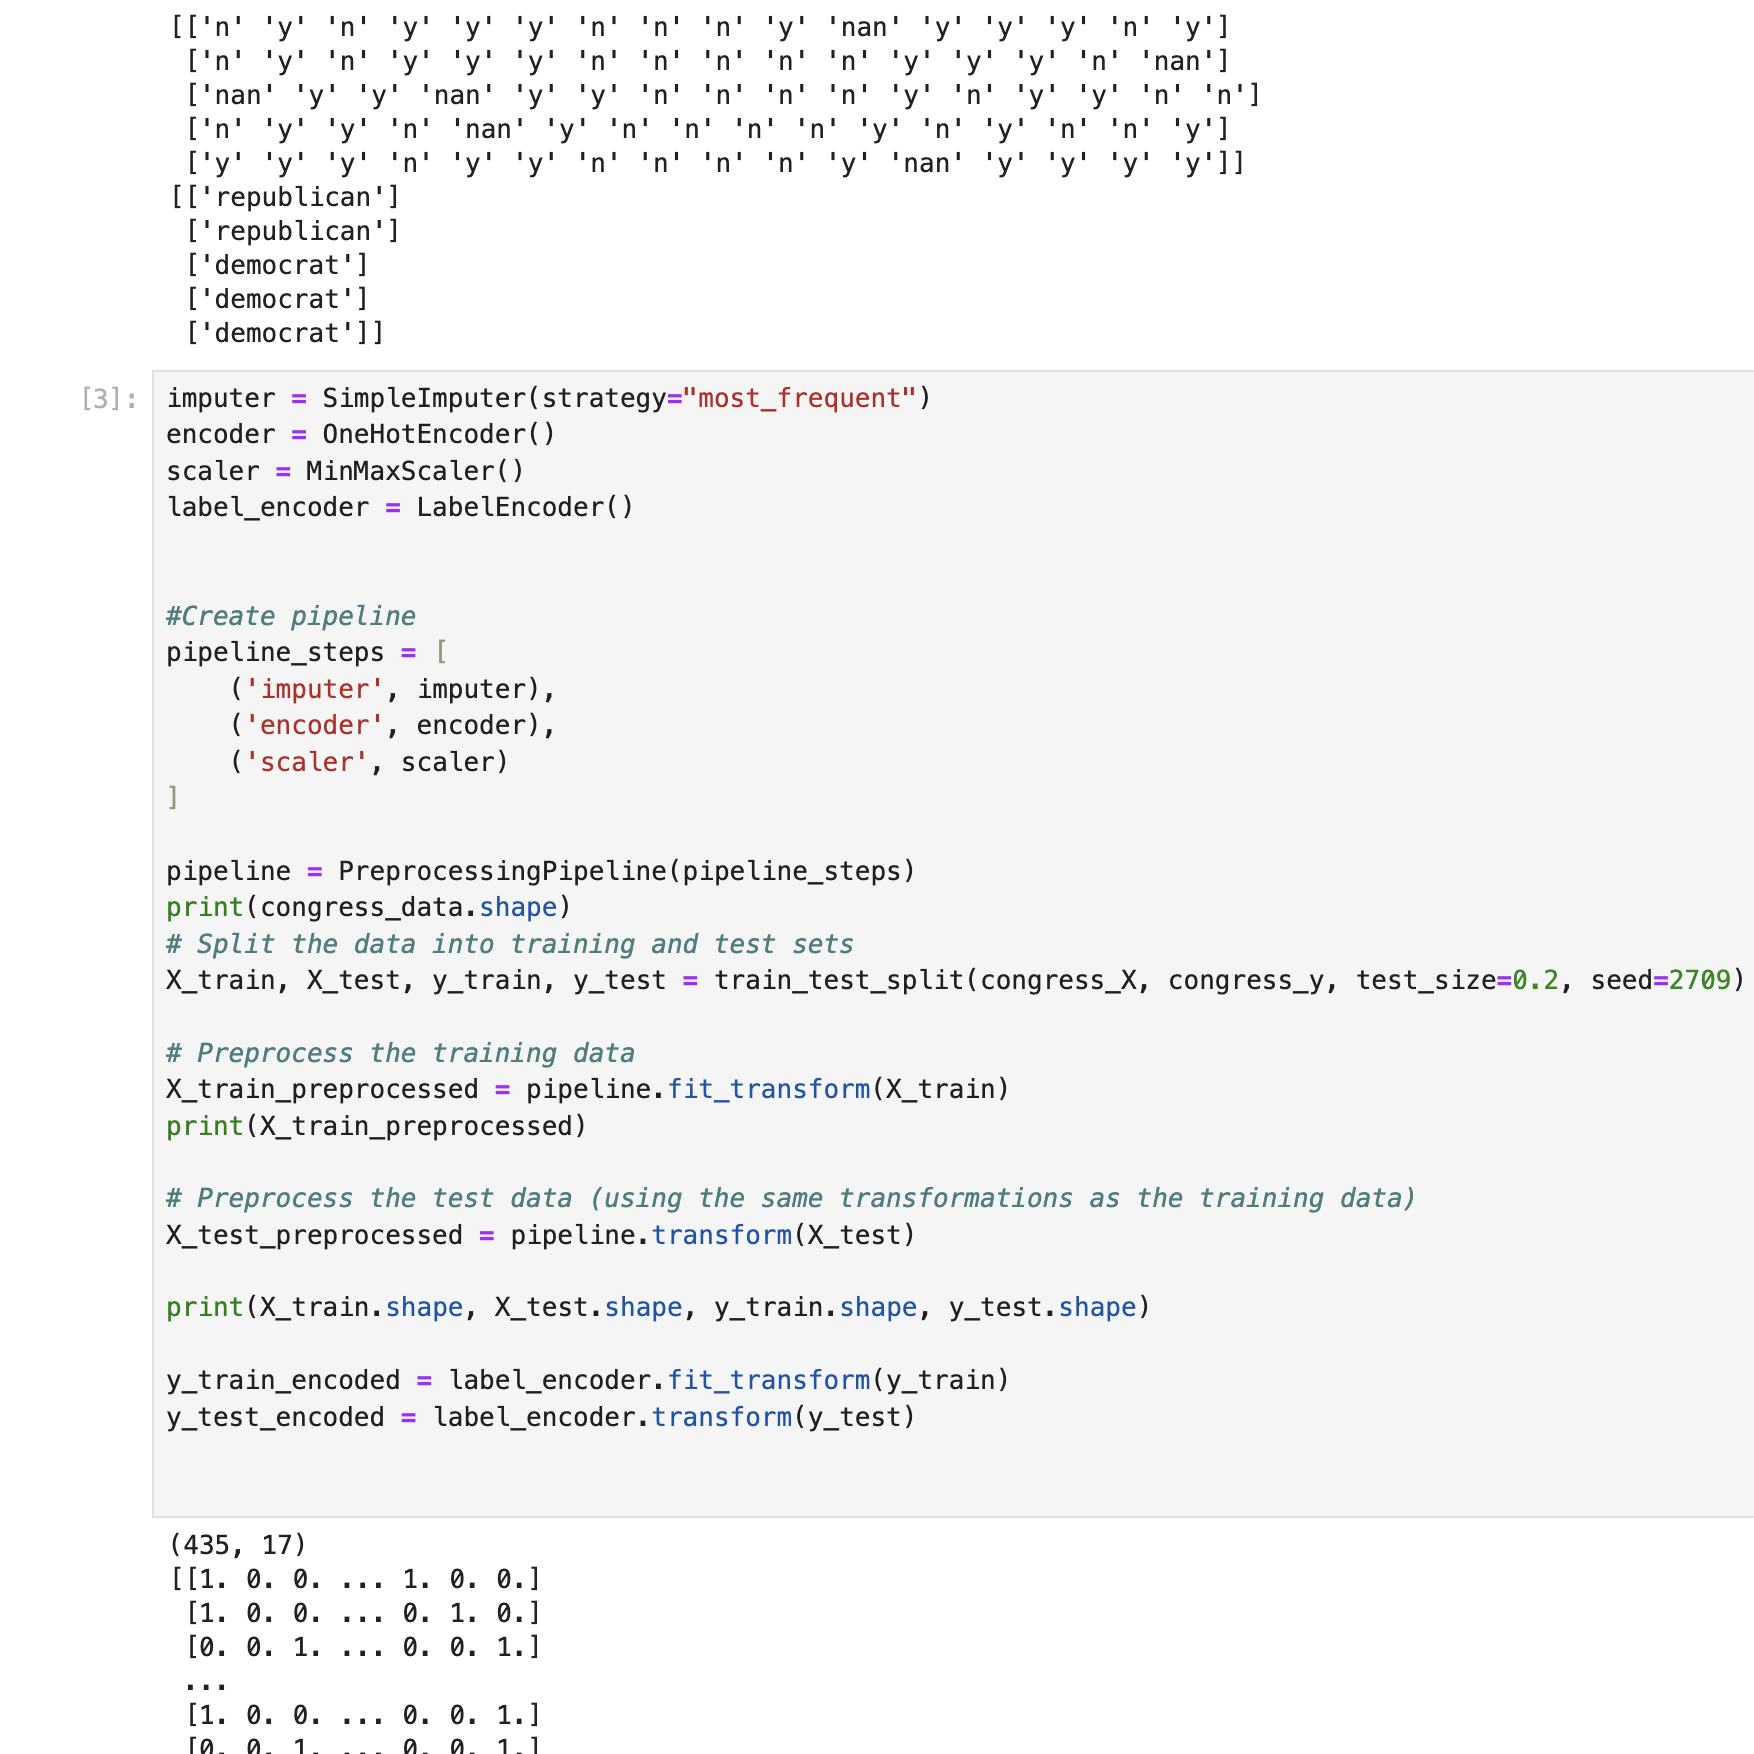
\includegraphics[width=0.8\textwidth]{notebook_9_excerpt.png}
    \caption{Notebook 9 - Congress dataset being handled with missing and categorical data}
    \label{fig:notebook_9}
\end{figure}

\subsubsection{Detecting Data Types - Technical Decision Compromise}

It's worth noting with all of this that it's important for the categorical, numerical and ordinal data columns to be identified to the application, with this implementation thus far. \par
At the end of Notebook 9, I experiment a little with a function I made called detect\_column\_types() which attempts to automatically determine if a column is numerical, categorical or ordinal using the uniqueness of values in a column and some thresholds to distinguish. I felt I was on an interesting path but I found it too easy to find datasets that didn't suit whichever criteria I set, so I abandoned the idea. \par
I settled on leaving the task of defining the data types of each column in the dataset to the user. \par

\subsection{Softmax Regression}
\subsubsection{Choosing Softmax}
I knew that two algorithms wouldn't be enough for the project to be complete. After asking my supervisor about it during my third and fourth meeting, I felt quite certain that logistic regression would be the third algorithm to pit against the previous two. I wanted to use a parametric model for sure and I noted that logistic regression had quite a lot of relevance in industry for classification. \par
However, I quickly noted that logistic regression is a binomial classification method - it can only handle two classes, so it wouldn't even be useful for iris dataset unless some adjustment was made to it. \par
A common approach is to utilise a One-vs-Rest or One-vs-One approach, a suggestion by my supervisor when asking during my fourth meeting. However this approach seemed to me, computationally expensive. I disliked the idea of generating multiple models and making them vote - it felt like a clunky compromise to me. \par 
After some research, I found that softmax regression was an elegant and challenging approach to making logistic regression a multi-class classifier. \par

\subsubsection{Implementing step-by-step} 
I struggled for a while to get things started, the softmax function seemed rather abstract to me at first - and I realised I was making the same mistake that I made when trying to implement the Decision Tree model, I was trying to build too much at once. \par
Within logistic\_regression.py I began working on an implementation of standard binomial logistic regression. I found that doing this drastically simplified things, despite knowing that this model wouldn't be used in my project. \par

\begin{lstlisting} [language=Python, caption=logistic\_regression.py - LogisticRegression] 
    class LogisticRegression:
    def __init__(self, learning_rate=0.01, n_iterations=1000):
        self.learning_rate = learning_rate
        self.n_iterations = n_iterations
        self.weights = None
        self.bias = None
        self.label_map = None
        self.loss_history = []  # To store the loss at each iteration

    def sigmoid(self, z):
        return 1 / (1 + np.exp(-z))
    
    def log_loss(self, y_true, y_pred):
        epsilon = 1e-15  # To prevent log(0)
        y_pred = np.clip(y_pred, epsilon, 1 - epsilon)
        return -np.mean(y_true * np.log(y_pred) + (1 - y_true) * np.log(1 - y_pred))
    
    def gradient_descent_step(self, X, y):
        n_samples, n_features = X.shape
        model = np.dot(X, self.weights) + self.bias
        predictions = self.sigmoid(model)

        dw = (1 / n_samples) * np.dot(X.T, (predictions - y))
        db = (1 / n_samples) * np.sum(predictions - y)

        self.weights -= self.learning_rate * dw
        self.bias -= self.learning_rate * db
        return predictions  # Return predictions for loss calculation

    def fit(self, X, y):
        # Check for more than two unique labels
        unique_labels = np.unique(y)
        if len(unique_labels) != 2:
            raise ValueError("Logistic Regression is a binary classifier and requires exactly 2 classes.")
        
        # Store mapping of unique labels to 0 and 1
        self.label_map = {unique_labels[0]: 0, unique_labels[1]: 1}
        mapped_y = np.vectorize(self.label_map.get)(y)
        
        n_samples, n_features = X.shape
        self.weights = np.zeros(n_features)
        self.bias = 0

        for _ in range(self.n_iterations):
            predictions = self.gradient_descent_step(X, mapped_y)
            loss = self.log_loss(mapped_y, predictions)
            self.loss_history.append(loss)

    def predict(self, X):
        model = np.dot(X, self.weights) + self.bias
        predictions = self.sigmoid(model)
        predicted_labels = [1 if i > 0.5 else 0 for i in predictions]
        
        # Map predicted labels back to original class labels
        inverse_label_map = {v: k for k, v in self.label_map.items()}
        original_labels = np.vectorize(inverse_label_map.get)(predicted_labels)
        
        return original_labels

\end{lstlisting}

I began working on the sigmoid function and worked my way outwards. The sigmoid function maps any real-valued number into the (0, 1) interval. This function is critical for converting the linear combination of inputs and weights into a probability. The log\_loss(y\_true, y\_pred) function computes the binary cross-entropy loss. It measures the performance of the model, with a lower loss indicating better performance. The use of np.clip within this function prevents log(0), which would result in NaN values, by setting a lower and upper bound on the predicted probabilities. \par
The model parameters are updated via the gradient\_descent\_step(X, y). This method calculates the gradient of the loss function with respect to the model's weights and bias, then adjusts these parameters in the direction that minimizes the loss. The learning rate controls the size of these adjustments. Loss values are tracked across iterations in loss\_history. \par

I actually tested out this model quite thoroughly in Notebook 8 (Figure: \ref{fig:notebook_8_1}), on altered versions of the iris dataset as well as the Bank Authentication~\cite{banknote_authentication} dataset, which it performed rather well on, given that it's a binary classification task. 

\begin{figure}[ht]
    \centering
    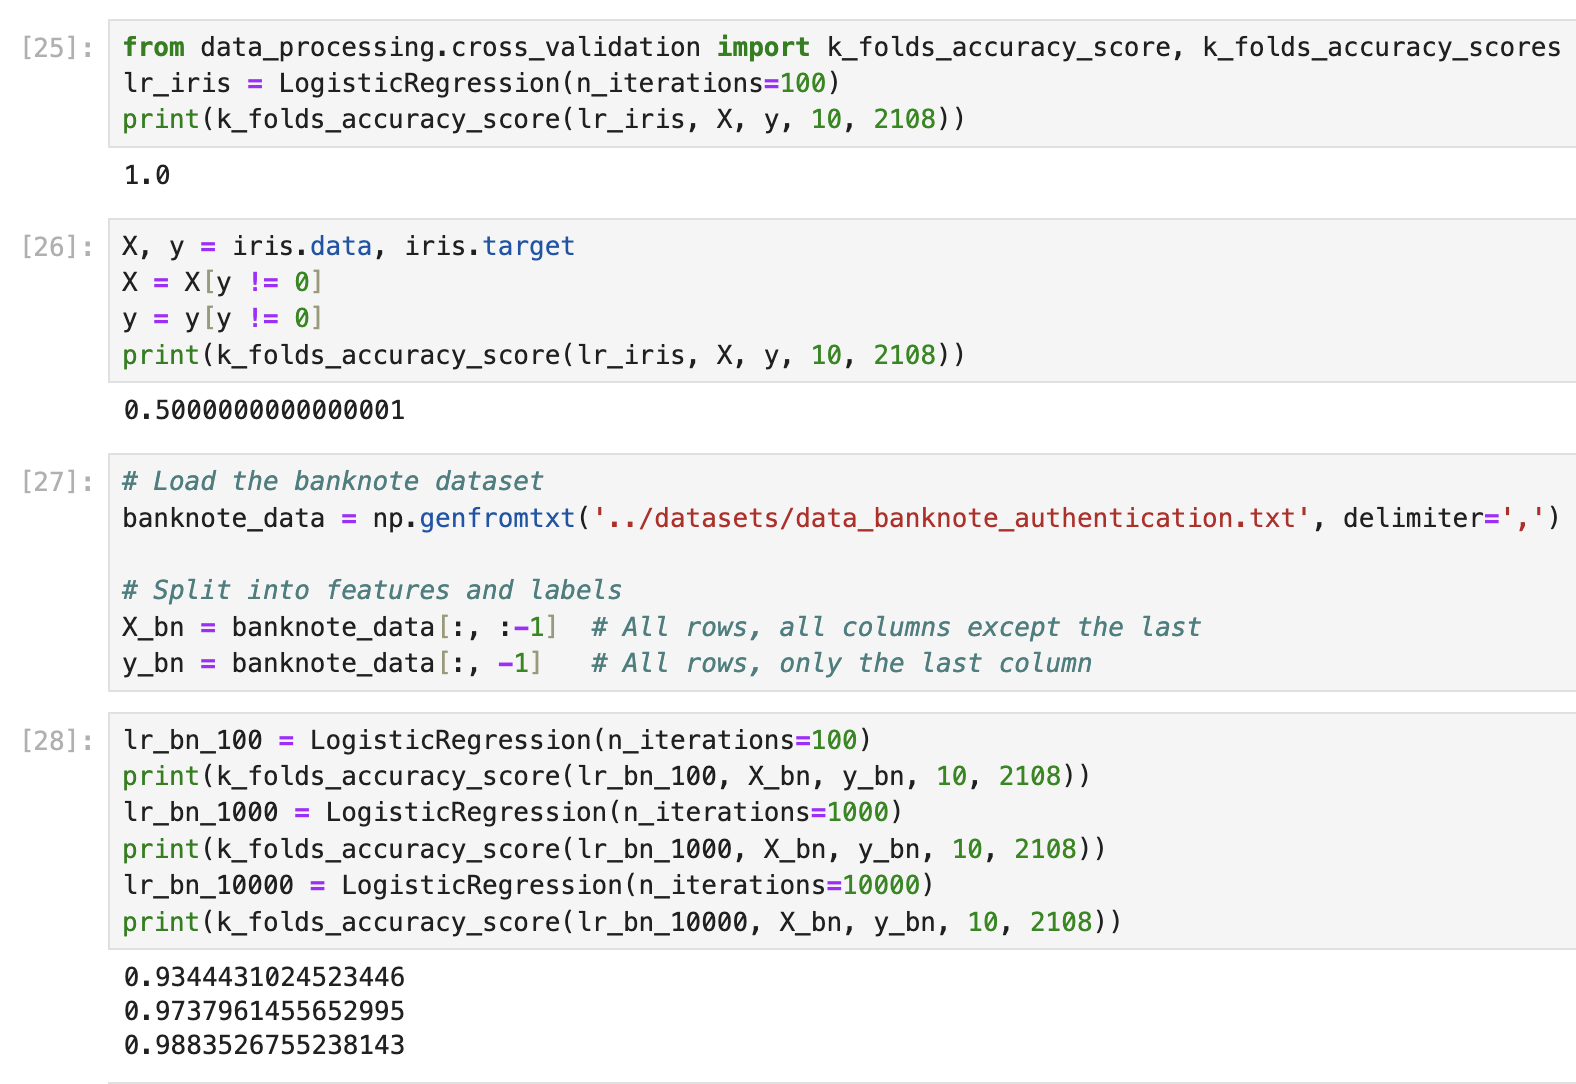
\includegraphics[width=0.8\textwidth]{notebook_8_bank.png}
    \caption{Notebook 8 - Logistic Regression in action}
    \label{fig:notebook_8_1}
\end{figure}

Building upon this, I began working on Softmax Regression. 

\begin{lstlisting}[language=Python, caption=logistic\_regression.py - SoftmaxRegression] 
    class SoftmaxRegression:
    def __init__(self, learning_rate=0.01, n_iterations=1000, lambda_=0.01):
        self.learning_rate = learning_rate
        self.n_iterations = n_iterations
        self.weights = None
        self.bias = None
        self.label_map = None
        self.loss_history = []  # To store the loss at each iteration
        self.name = "Softmax Regression"
        self.lambda_ = lambda_  # Regularization strength

    def softmax(self, z):
        e_z = np.exp(z - np.max(z, axis=1, keepdims=True))
        return e_z / np.sum(e_z, axis=1, keepdims=True)
    
    def compute_loss(self, y_true, y_pred):
        epsilon = 1e-15  # To prevent log(0)
        y_pred_clipped = np.clip(y_pred, epsilon, 1 - epsilon)
        cross_entropy_loss = -np.mean(np.sum(y_true * np.log(y_pred_clipped), axis=1))
        l2_penalty = (self.lambda_ / 2) * np.sum(np.square(self.weights))
        total_loss = cross_entropy_loss + l2_penalty
        return total_loss

    def gradient_descent_step(self, X, y_one_hot, probabilities):
        n_samples = X.shape[0]
        dw = (1 / n_samples) * np.dot(X.T, (probabilities - y_one_hot))
        db = (1 / n_samples) * np.sum(probabilities - y_one_hot, axis=0, keepdims=True)
        
        dw += self.lambda_ * self.weights
        
        self.weights -= self.learning_rate * dw
        self.bias -= self.learning_rate * db

    def fit(self, X, y, print_loss=False):
        unique_labels = np.unique(y)
        self.label_map = {original_label: i for i, original_label in enumerate(unique_labels)}

        mapped_y = np.vectorize(self.label_map.get)(y)
        
        n_samples, n_features = X.shape
        n_classes = len(unique_labels)

        self.weights = np.zeros((n_features, n_classes))
        self.bias = np.zeros((1, n_classes))
        self.loss_history = []  # Reset loss history for each fit call
        
        y_one_hot = np.eye(n_classes)[mapped_y]

        for i in range(self.n_iterations):
            scores = np.dot(X, self.weights) + self.bias
            probabilities = self.softmax(scores)
            
            loss = self.compute_loss(y_one_hot, probabilities)
            self.loss_history.append(loss)
            
            self.gradient_descent_step(X, y_one_hot, probabilities)
            
            if i % 100 == 0 and print_loss:
                print(f"Iteration {i}: Loss {loss}")
    
    def predict(self, X):
        scores = np.dot(X, self.weights) + self.bias
        probabilities = self.softmax(scores)
        predicted_classes = np.argmax(probabilities, axis=1)
        
        inverse_label_map = {i: original_label for original_label, i in self.label_map.items()}
        original_labels = np.vectorize(inverse_label_map.get)(predicted_classes)
        
        return original_labels
\end{lstlisting}

This final implementation also makes use of L2 Regularization to prevent overfitting during training. This is also demonstrated in Notebook 8.\par

\begin{figure}[ht]
    \centering
    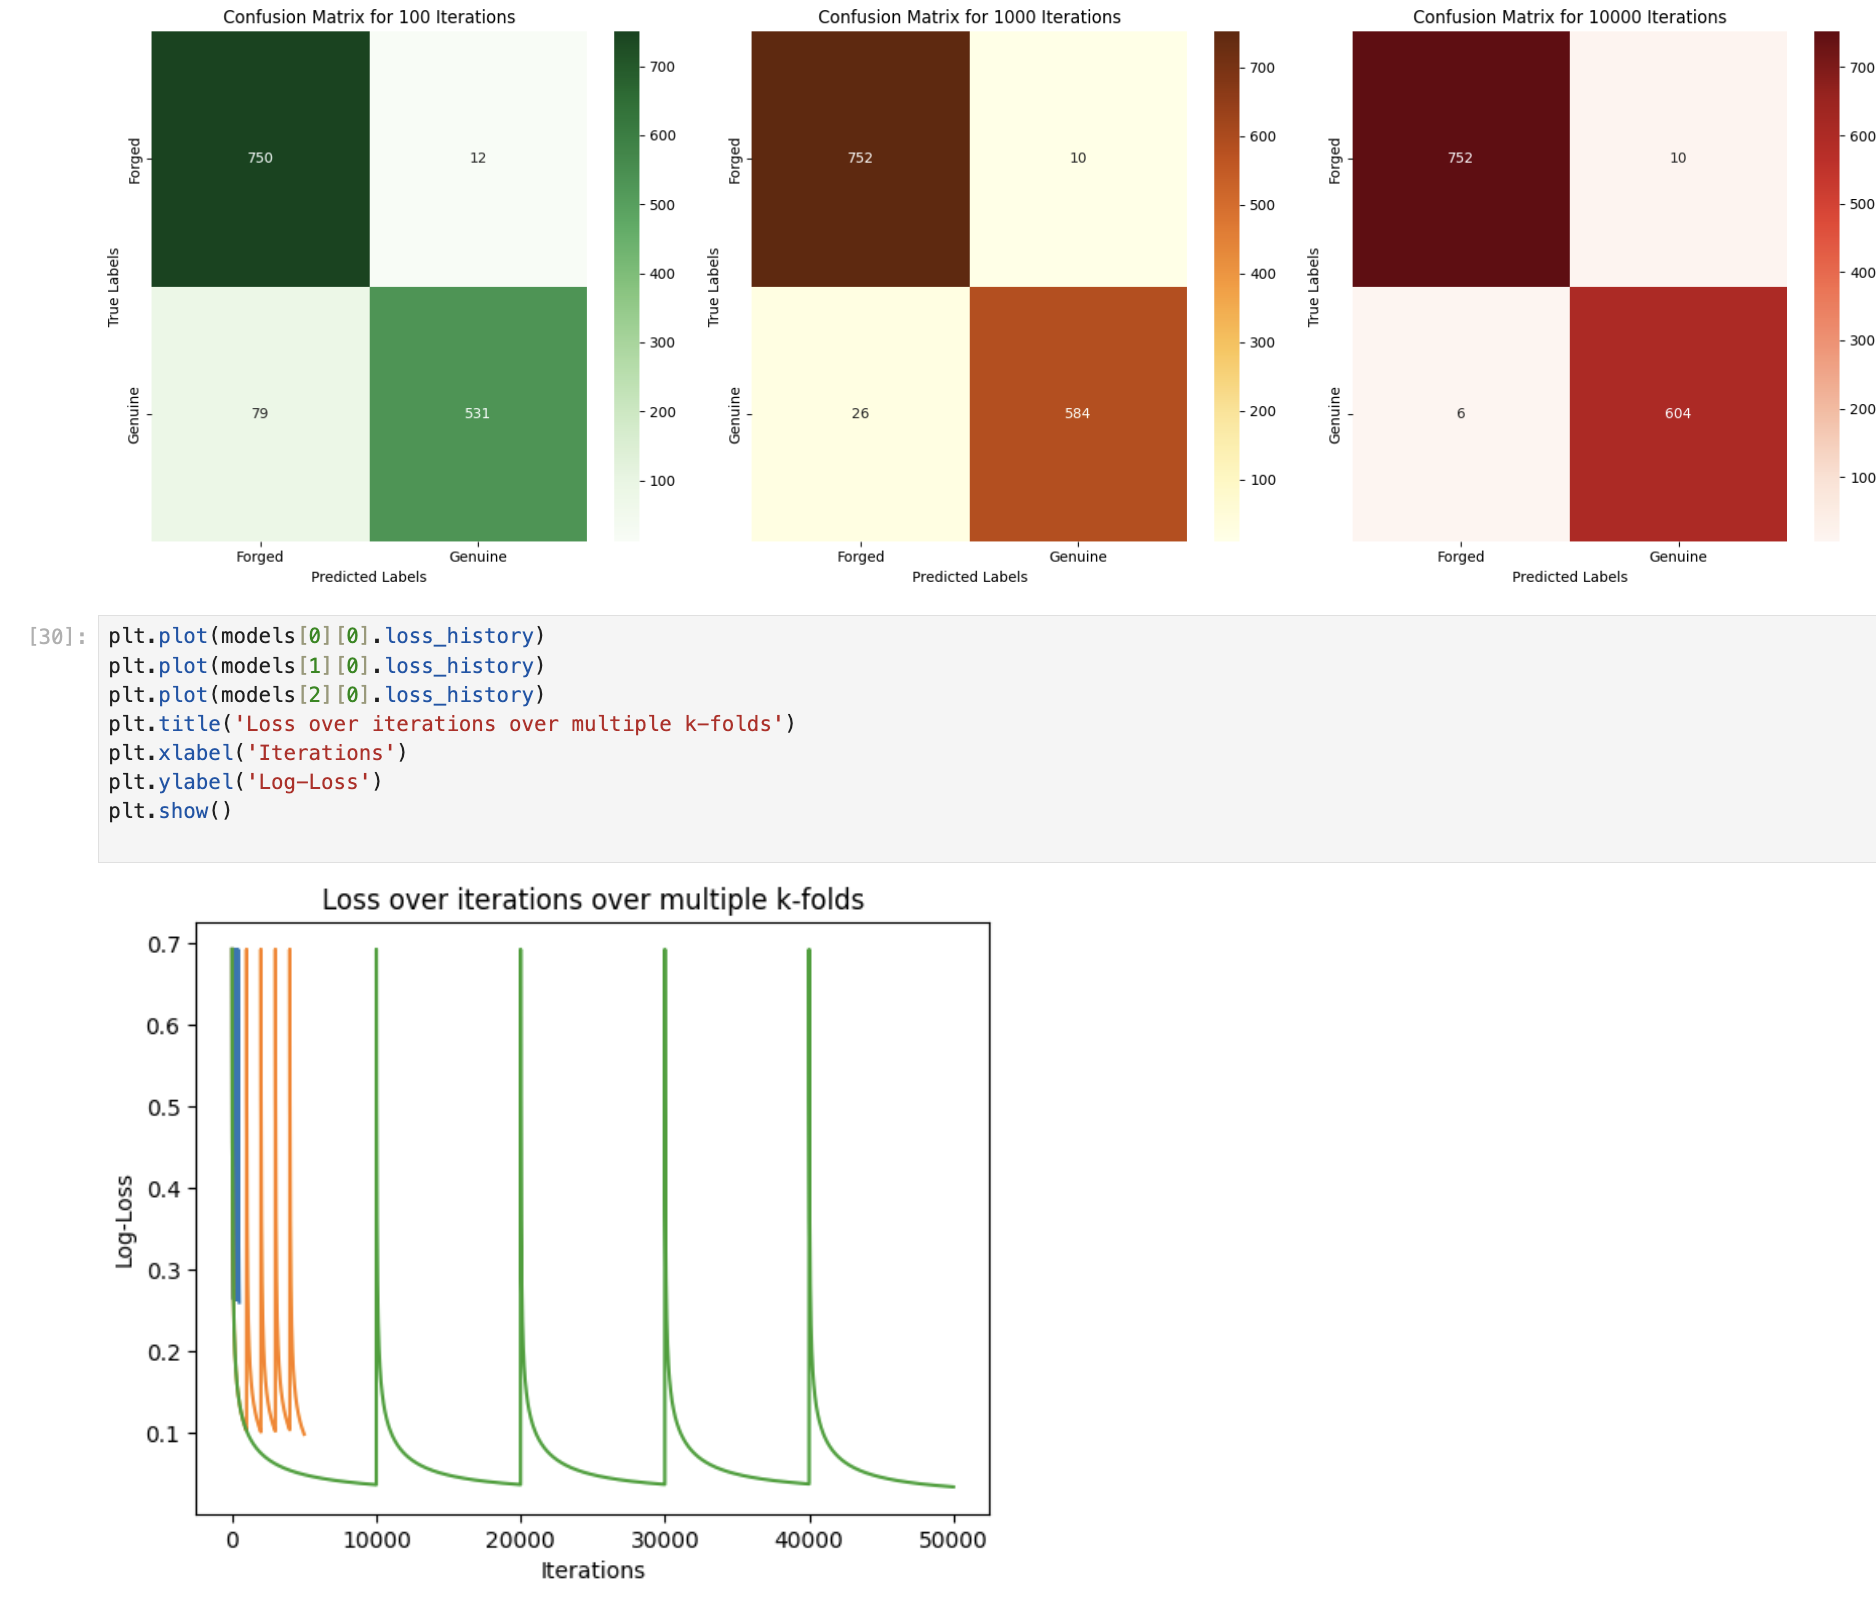
\includegraphics[width=0.8\textwidth]{notebook_8_loss.png}
    \caption{Notebook 8 - Number of iterations against the loss}
    \label{fig:notebook_8_2}
\end{figure}

\newpage
\subsection{Model Tuning}
We have our models and we have our processed data, however we now need to dive into the tuning process of our models. I noted during my interim review notebook in December, that a very large amount of my notebook was taken up by code that was made in an effort to find the most optimally tuned models to be used for training, comparison and evaluation. \par
The most obvious thing to do, was to implement an exhaustive grid search class that could retrieve a model with a dataset and spit back an ideal model with its optimally set hyper-parameters. It would need to know which model has been retrieved and set it a parameter grid, and a default parameter grid would need to be defined for each of the three models. \par
\subsubsection{Grid Search}
Below is my implementation within the optimisers.py module. This file is within the models subdirectory.

\begin{lstlisting}[language=Python, caption=optimisers.py - GridSearch]
    class GridSearch:
    def __init__(self, model, param_grid=None, scoring=None):
        self.model = model
        if param_grid is None:
            self.param_grid = self._get_default_param_grid()
        else:
            self.param_grid = param_grid
        self.scoring = scoring
        self.best_params_ = None
        self.best_score_ = None
        self.best_model_ = None
        self.scores_ = []

    def fit(self, X_train, y_train, X_val, y_val):
        params_list = self._generate_params_list()
        scores = []

        for params in params_list:
            model = self._clone_model()
            model.__init__(**params)
            model.fit(X_train, y_train)
            score = self._validate(model, X_val, y_val)
            scores.append(score)

            if self.best_score_ is None or score > self.best_score_:
                self.best_score_ = score
                self.best_params_ = params
                self.best_model_ = model

        self.scores_ = scores

    def _clone_model(self):
        return self.model.__class__()

    def _generate_params_list(self):
        param_names = list(self.param_grid.keys())
        param_values = list(self.param_grid.values())
        params_list = [dict(zip(param_names, params)) for params in product(*param_values)]
        return params_list
    
    def _get_default_param_grid(self):
        if isinstance(self.model, KNearestNeighbours):
            param_grid = {'k': [1, 3, 5, 7, 9, 10, 15]}
        elif isinstance(self.model, ClassificationTree):
            param_grid = {'max_depth': [3, 5, 10, 15, 20], 'min_size': [2, 5, 10, 20]}
        elif isinstance(self.model, SoftmaxRegression):
            param_grid = {'n_iterations': [100, 500, 1000, 5000], 'learning_rate': [0.001, 0.01, 0.1, 1]}
        else:
            raise ValueError(f"Unsupported model type: {type(self.model)}")

        return param_grid

    def _validate(self, model, X_val, y_val):
        if self.scoring is None:
            y_pred = model.predict(X_val)
            score = np.mean(y_pred == y_val)
        else:
            score = self.scoring(model, X_val, y_val)

        return score

    def score(self, X, y):
        if self.scoring is None:
            y_pred = self.best_model_.predict(X)
            score = np.mean(y_pred == y)
        else:
            score = self.scoring(self.best_model_, X, y)

        return score

    def get_params(self, deep=True):
        return {
            'model': self.model,
            'param_grid': self.param_grid,
            'scoring': self.scoring
        }
    
    def get_scores(self):
        return self.scores_

    def set_params(self, **params):
        for param, value in params.items():
            setattr(self, param, value)
        return self

    def display_param_grid(self):
        print("Parameter Grid:")
        for param, values in self.param_grid.items():
            print(f"{param}: {values}")
    
    def plot_param_grid_heatmap(grid_search):
        param_grid = grid_search.param_grid
        scores = grid_search.scores_
        param_combinations = []
        for params in grid_search._generate_params_list():
            param_combinations.append(tuple(params.values()))
        scores_array = np.array(scores).reshape(-1, 1)

        if len(param_grid) == 1:
            plt.figure(figsize=(8, 6))
            param_name = list(param_grid.keys())[0]
            param_values = [pc[0] for pc in param_combinations]
            plt.plot(param_values, scores, marker='o', linestyle='-')
            plt.title('Grid Search Scores')
            plt.xlabel(param_name)
            plt.ylabel('Score')
            plt.xticks(rotation=45)
            plt.grid(True)
            plt.tight_layout()
        else:
            param_combinations_array = np.array(param_combinations)
            param_names = list(param_grid.keys())
            param_values = [np.unique(param_combinations_array[:, i]) for i in range(len(param_names))]
            scores_table = np.zeros((len(param_values[0]), len(param_values[1])))
            for i in range(len(param_combinations)):
                row_idx = np.where(param_values[0] == param_combinations[i][0])[0][0]
                col_idx = np.where(param_values[1] == param_combinations[i][1])[0][0]
                scores_table[row_idx, col_idx] = scores[i]

            plt.figure(figsize=(8, 6))
            sns.heatmap(scores_table, annot=True, cmap='coolwarm', fmt='.3f',
                        xticklabels=param_values[1], yticklabels=param_values[0],
                        cbar_kws={'label': 'Score'})
            plt.title('Grid Search Scores')
            plt.xlabel(param_names[1])
            plt.ylabel(param_names[0])
            plt.tight_layout()

        plt.show()

\end{lstlisting}

The class initialises with a model object, a parameter grid, and an optional scoring function. If no parameter grid is provided, a default one is determined based on the model type. The class provides functionalities including fitting models with training and validation datasets to find the best hyperparameters, cloning models to ensure each parameter combination is evaluated independently, and generating all possible parameter combinations. Additionally, it supports default parameter grids for certain model types (e.g., KNearestNeighbours, ClassificationTree, SoftmaxRegression), and offers a method to validate model performance on a validation dataset.

The GridSearch class also includes methods for obtaining the best model's score on given data, getting and setting parameters of the grid search object, and displaying the parameter grid. Notably, it features a method to plot a heatmap of scores for each parameter combination, facilitating the visualization of how different parameters affect model performance. This module leverages libraries such as NumPy, pandas, Matplotlib, and Seaborn for data manipulation and visualization, and assumes model classes like KNearestNeighbours, ClassificationTree, SoftmaxRegression follow a consistent interface for fitting and prediction.

\subsection{Small Tree Split Optimisation}
Before moving onto the the GUI, I did have an goal to optimise the tree training process. At the beginning of the second term, I did manage to change a single line in the get\_split() function that quite drastically improved computational performance. I've shown this in Figure \ref{tree_optimisation}\par

\begin{figure}[ht]
    \centering
    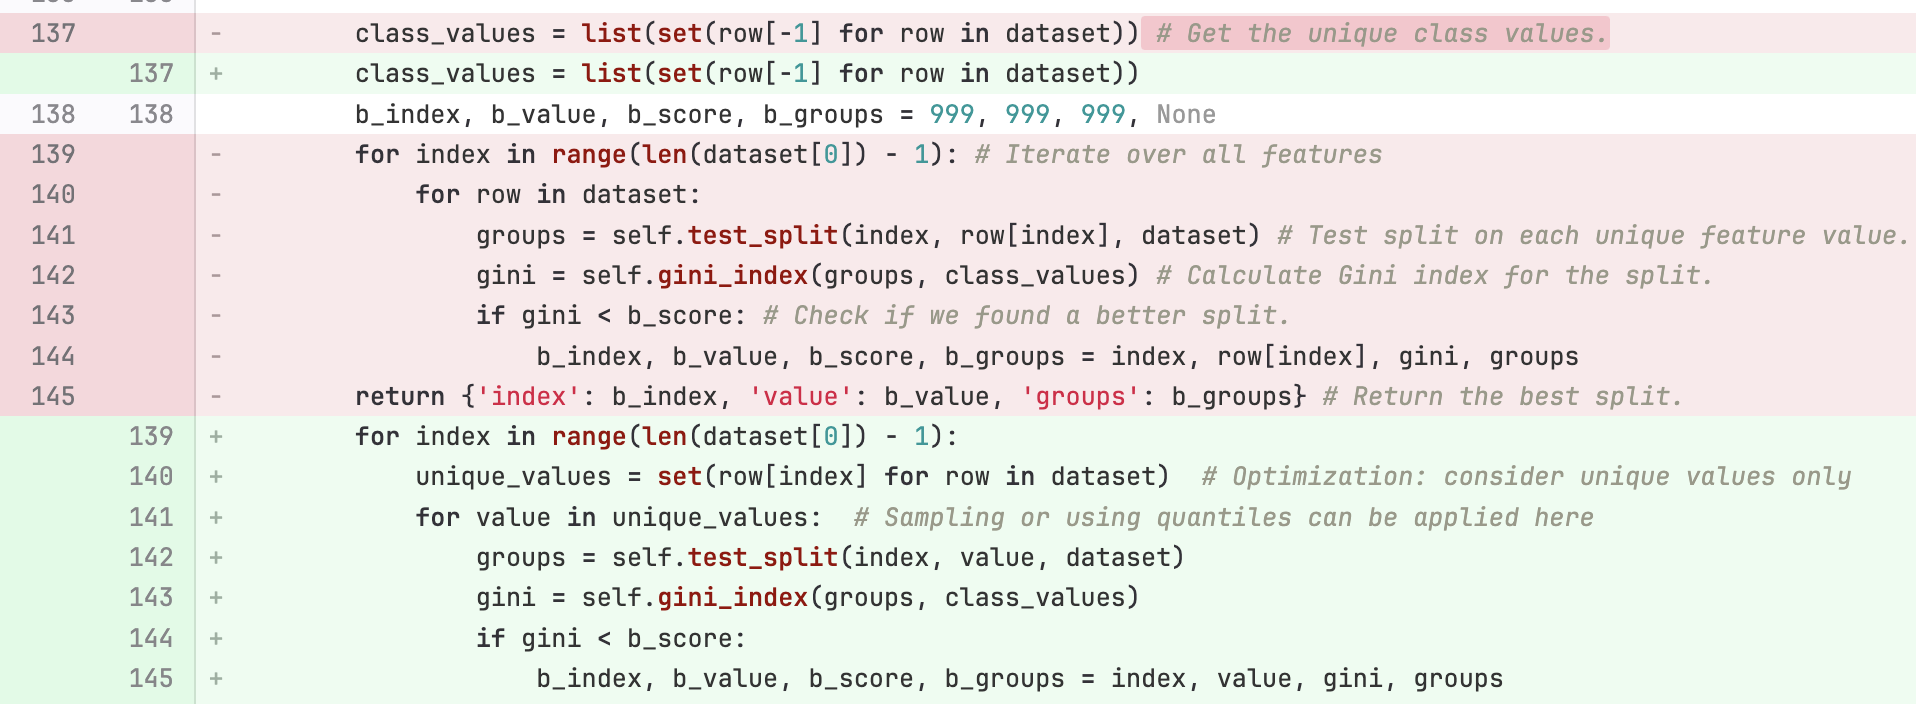
\includegraphics[width=0.8\textwidth]{tree_optimisation.png}
    \caption{Small optimisation in tree-splitting function}
    \label{tree_optimisation}
\end{figure}

The original code iterated over every value in each feature, leading to redundant calculations when multiple rows had the same value for a feature. By introducing a set, we only evaluate over unique values. This is such a trivial change but it made working with the tree model far less sluggish. As my comments suggest, there was an opportunity to improve this further with sampling and quantiles but I didn't find the time to extend this much more. \par

\subsection{Metrics}
Accuracy was not enough to evaluate the models, and I wanted to implement a metrics module that could calculate important and usable metrics when given a confusion matrix to examine. I implemented this quite quickly in metrics.py and demonstrated this in the final Jupyter notebook, Notebook 11. \par
Notebook 11 also demonstrates virtually all of my backend logic in one neat code block, on the challenging Titanic dataset. It's a good notebook to refer to. \par

\begin{figure}
    \centering
    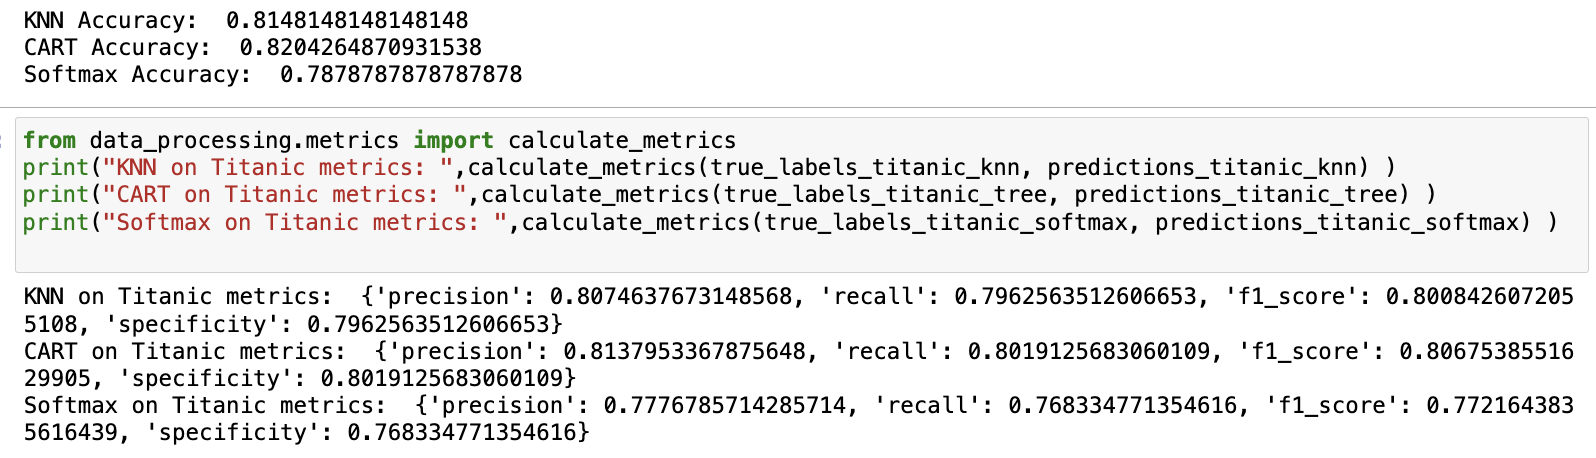
\includegraphics[width=0.9\linewidth]{notebook11_metrics.png}
    \caption{Notebook 11 - Calcluating the metrics from a confusion matrix}
    \label{fig:notebook11_metrics}
\end{figure}

\subsection{GUI and Standalone Application}
And finally with everything in place, it was time to work on the interface. Much of the prior work took place on a Git branch named 'dev-poc' for Proof-Of-Concept. I began developing my interface on a new branch, just in case I needed these workflows to be in separate spaces. \par


\subsubsection{Initial Interface and File Loading}
My initial effort on the interface involved simply laying out the layout and buttons for loading and training on the dataset, and getting familiar with PyQT5. My initial commit of the interface simply implements an interface that utilises the file-loading function (section \ref{fileloading}) and displaying the first five lines of the dataset to show it worked. This is still present in the final implementation, and gives a decent preview of the data loading and preprocessing (or pre-preprocessing) in action. 

\begin{lstlisting}[language=Python, caption=ui.py - Initial Effort with file loading. Mostly a dummy interface.]
    import sys
from PyQt5.QtWidgets import QApplication, QWidget, QLabel, QLineEdit, QPushButton, QVBoxLayout, QHBoxLayout, QFileDialog, QMessageBox
from PyQt5.QtCore import Qt
from preprocessing import load_dataset

class MainWindow(QWidget):
    def __init__(self):
        super().__init__()
        self.setWindowTitle('Dataset Loader')
        self.setGeometry(100, 100, 400, 300)  
        self.init_ui()
    
    def init_ui(self):
        layout = QVBoxLayout()

        file_layout = QHBoxLayout()
        self.file_label = QLabel('Dataset File:')
        self.file_text = QLineEdit()
        self.file_button = QPushButton('Browse')
        self.file_button.clicked.connect(self.browse_file)
        file_layout.addWidget(self.file_label)
        file_layout.addWidget(self.file_text)
        file_layout.addWidget(self.file_button)

        self.load_button = QPushButton('Load Dataset')
        self.load_button.clicked.connect(self.load_dataset)

        self.preview_label = QLabel('')
        self.preview_label.setAlignment(Qt.AlignLeft | Qt.AlignTop)
        self.preview_label.setWordWrap(True)

        self.train_button = QPushButton('Train Models')
        self.train_button.setEnabled(False)
        self.train_button.clicked.connect(self.train_models)

        layout.addWidget(self.load_button)
        layout.addWidget(self.preview_label)  # Add the preview label to the layout
        layout.addLayout(file_layout)
        layout.addWidget(self.load_button)
        layout.addWidget(self.train_button)

        self.setLayout(layout)
    
    def browse_file(self):
        options = QFileDialog.Options()
        file_path, _ = QFileDialog.getOpenFileName(self, 'Select Dataset File', '', 'All Files (*)', options=options)
        if file_path:
            self.file_text.setText(file_path)
    
    def load_dataset(self):
        file_path = self.file_text.text()
        if file_path:
            # Load the dataset using the load_dataset function
            X, y = load_dataset(file_path)
            QMessageBox.information(self, 'Dataset Loaded', 'Dataset has been loaded successfully.')
            self.train_button.setEnabled(True)

            # Display the first five lines of the loaded dataset
            preview_text = 'Dataset Preview:\n'
            for i in range(min(5, len(X))):
                preview_text += f'Line {i+1}: {X[i]}\n'
            self.preview_label.setText(preview_text)
        else:
            QMessageBox.warning(self, 'No File Selected', 'Please select a dataset file.')
    
    def train_models(self):
        # Train the models here using the loaded dataset
        QMessageBox.information(self, 'Training Complete', 'Models have been trained successfully.')
    

def main():
    app = QApplication(sys.argv)
    window = MainWindow()
    window.show()
    sys.exit(app.exec_())

if __name__ == '__main__':
    main()

\end{lstlisting}

\subsubsection{Cross-Validation and Confusion Matrics}
Within a few hours of this commit, I managed to import and implement my k-folds cross-validation methodologies into the interface such that the interface now evaluated three models. I made a FigureCanvas class which displayed three confusion matrices side-by side. This implementation used a temporary constant combined preprocessor in the back-end but managed to work on 5-Folds Cross-Validation with affirmative results. \par
This implementation was limited to numeric datasets for the time-being. \par

\subsubsection{Threading and Abort}
It didn't take long until I realised that my app would need to implement threading - otherwise the interface will freeze for as long as the models are being trained (or tuned). I implemented a TrainingThread using QThread and pyqtSignals that was initiated when the Train Models button was pressed, and this handled the machine learning backend while the interface remained scrollable. \par
I also implemented an 'Abort' button around this time for when training was erroneously started or taking too long. \par

\subsubsection{Progress Bar}
I added a progress bar shortly after, whilst working on the threads. This progress bar served to indicate how many (out of three) of the models had finished training or tuning before full completion

\subsubsection{Complete Preprocessing}
I was working on the CombinedPreprocessor somewhat concurrently with the UI implementation, and at this point I had managed to complete the preprocessing on the poc branch of development. \par
For this commit, I managed to implement a "Process Data" button which prompted the user with dialog boxes for each data type, asking for column numbers. This worked sufficiently with the data but the user experience was very ugly and cumbersome with the pop up boxes, so this was abandoned. \par
During this time, the titanic dataset was the benchmark dataset to use, with missing data and all three data types in the dataset. \par

\subsubsection{Model Tuning}
Following the preprocessing breakthrough, I implemented my model tuning logic from the optimisers module and a "Tune Models" button. The UI now displayed the hyperparameters of the best model and used this model when "Train Models" was clicked. The results being displayed were now relatively comparable. 

\subsubsection{Column Input Boxes}
The dialog boxes were replaced with input boxes before the file selection and loading area, allowing the user to take their time with inputting where each data type of the dataset was located. 

\subsubsection{Multi-Threading and GridSearch Display}
To speed things up, my application uses multiple threads for each model such that each model is tuned asynchronously. This was a little challenging to implement at first but it seems to work smoothly. I also made a TuningPlotWidget which finally displayed the GridSearch for the Tree and Softmax Regression Models and a line graph for the performance of KNN. 

\subsubsection{Additional Touches}
By this point the next few commits were geared towards making the experience smoother. The progress bar was synchronised with both the tuning and training process and the abort button worked for both processes as well. Exception handling was added through the interface to prevent crashes and a metrics display was added to the bottom to present more results than just accuracy below the confusion matrices. \par

\subsection{Design Pattern - MVC}
At this stage in development, my ui.py file - which contained virtually the entire UI implementation of the application, was becoming rather bloated at almost 700 lines. More critically, this file had a mixture of backend logic with front-end UI elements. The lack of separation of concerns and the increasing complexity of the codebase prompted the need for refactoring. \par

Recognizing the opportunity to improve the project's architecture, the Model-View-Controller (MVC) design pattern was adopted. The MVC pattern promotes a clear separation of responsibilities, enhancing code organization, maintainability, and reusability. The refactoring process involved carefully analyzing the existing codebase and identifying the components that belonged to each layer of the MVC pattern. \par

\subsubsection{Model-View-Controller}

\begin{figure}[ht]
    \centering
    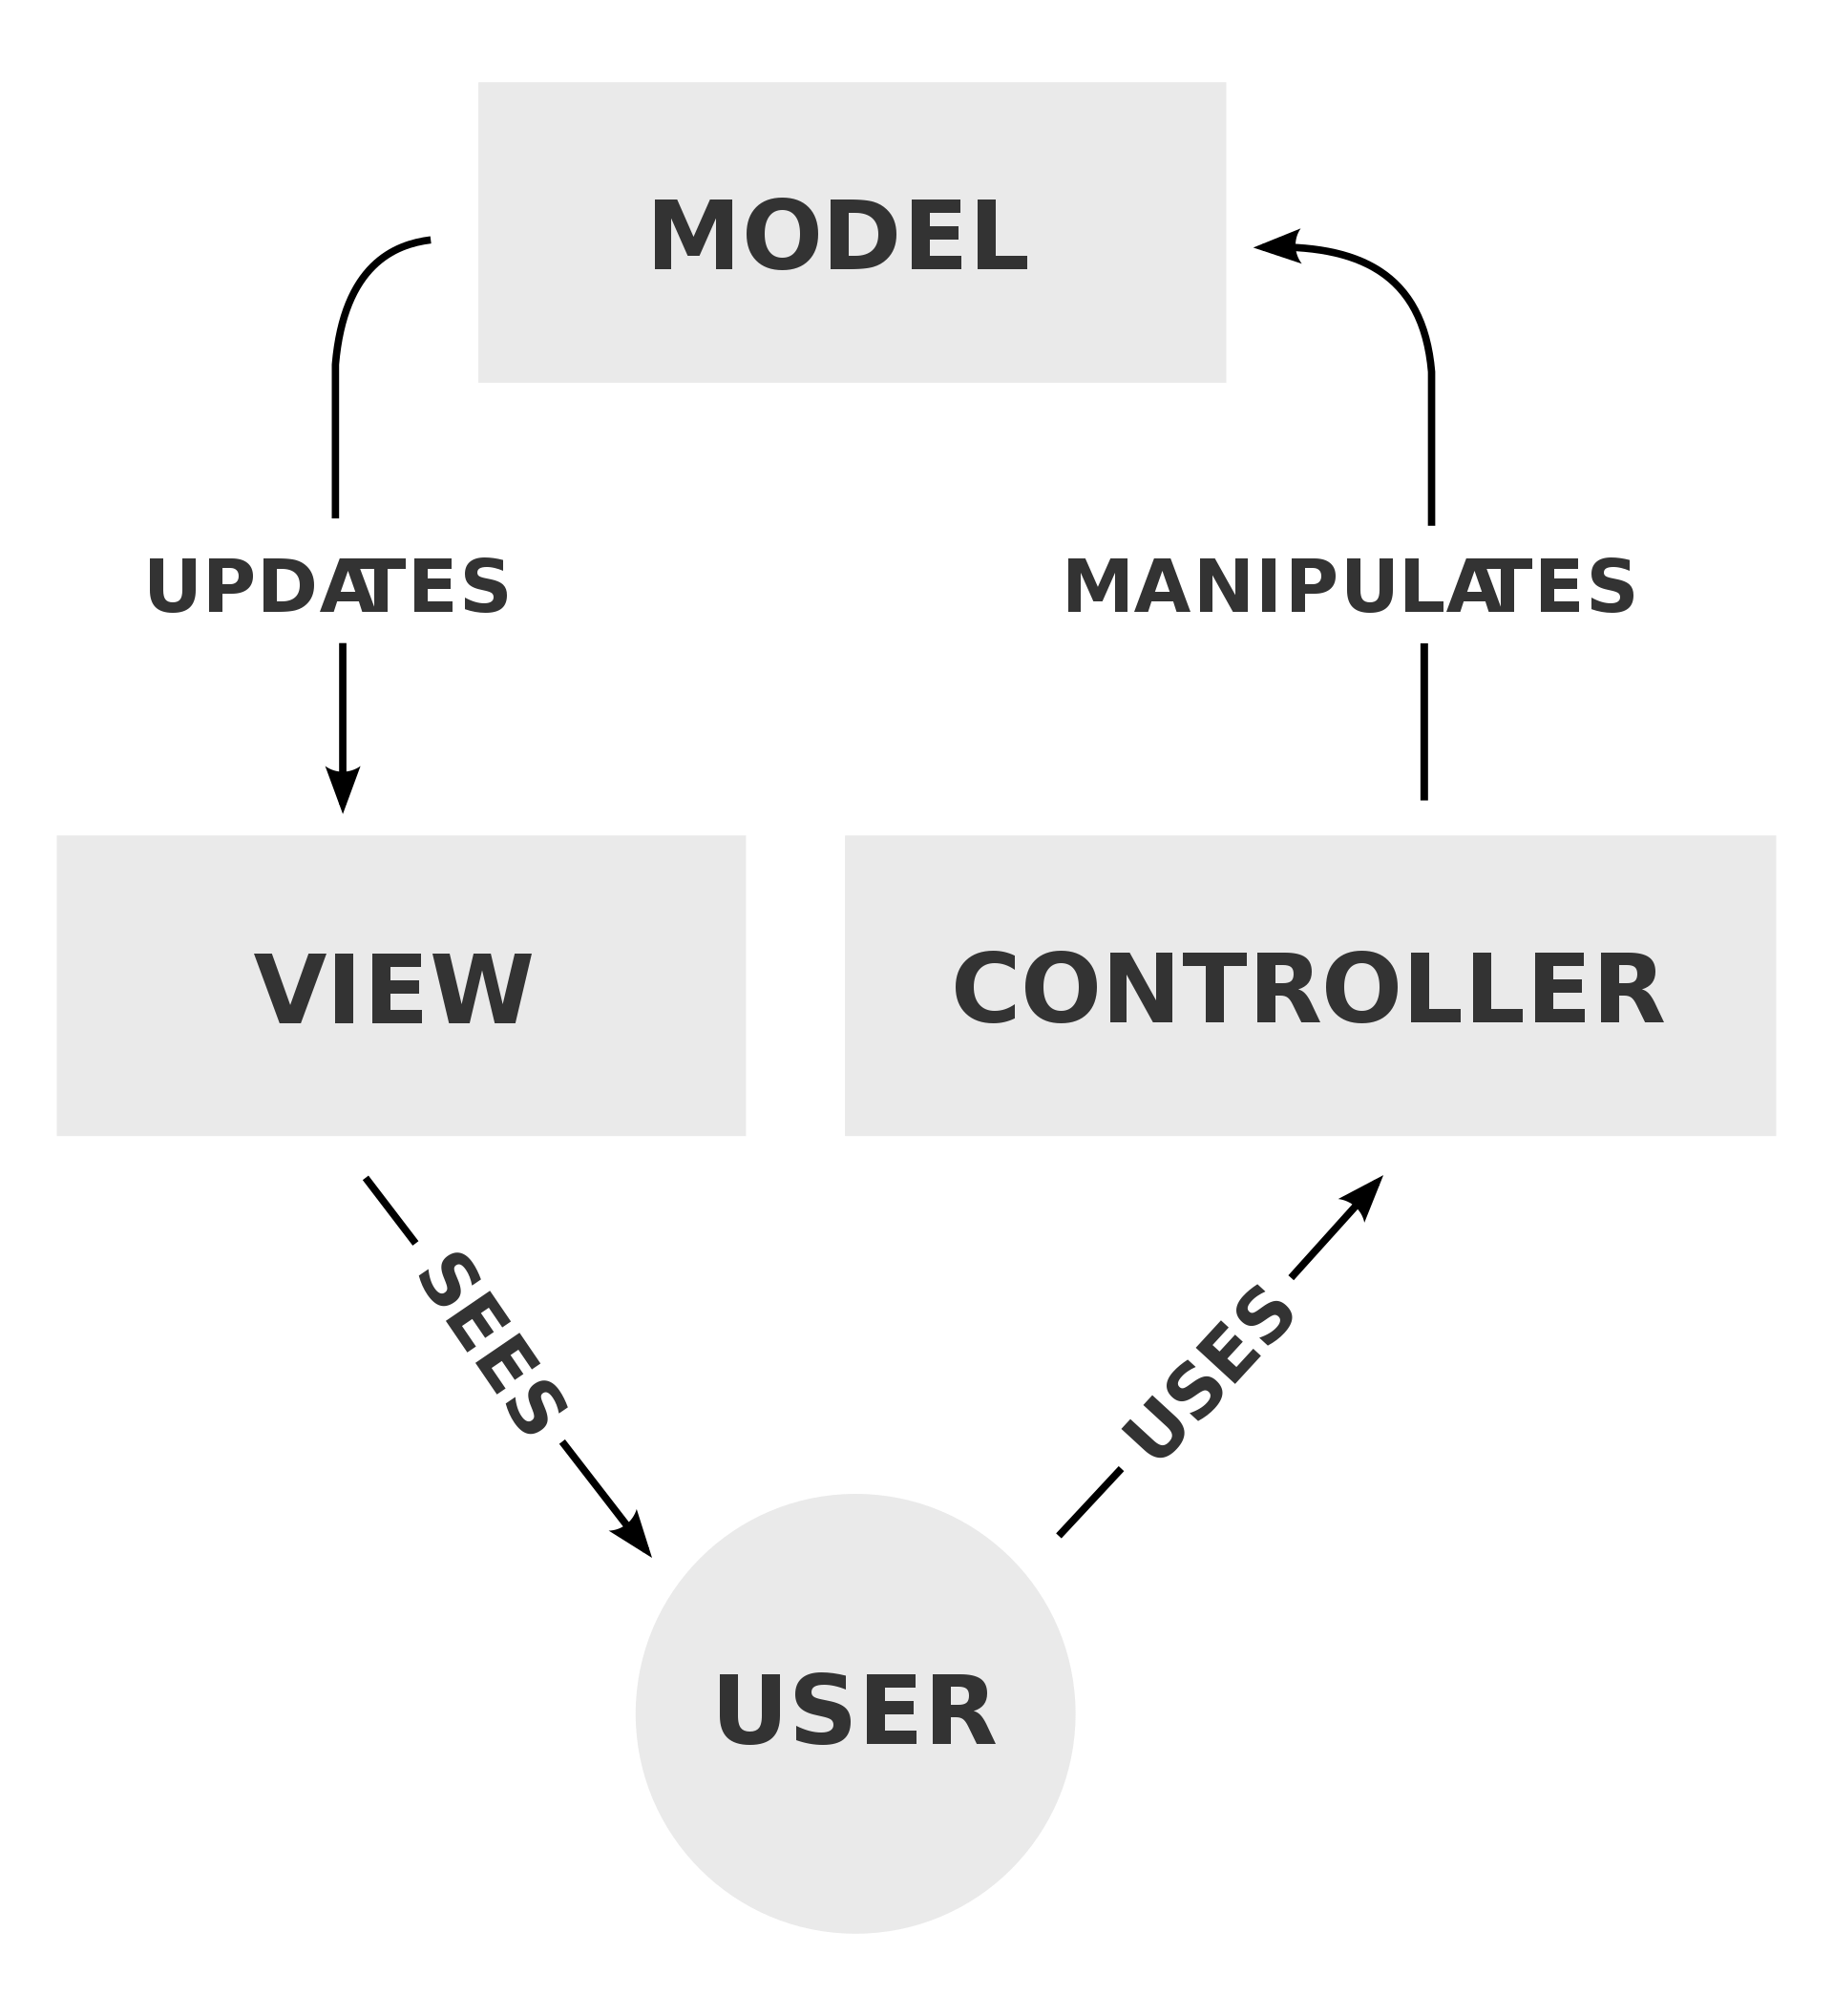
\includegraphics[width=0.6\textwidth]{MVC.png}
    \caption{The Model-View-Controller Design Pattern}
    \label{MVC}
\end{figure}

In this project, the Model represents the modules containing the machine learning models, the preprocessing modules and the metrics calculation functions - all the backend logic. \par
The View would obviously represent the interface and UI elements that the user directly interacts with, the buttons, labels and graph plots. \par
The Controller acts as the intermediary between these two, handling user actions, triggering Model operations and updating the View. 

\subsubsection{Refactoring}
Much of my refactoring, with this in mind, involved decoupling the controller from the view, taking backend logic away from the UI and into a new controllers module in my code. I shifted some other UI elements into files of their own and kept the UI elements in a module of their own too. \par
By the end of the refactoring, ui.py managed to look like this.

\begin{lstlisting}[language=Python, caption=ui.py - Final structure after refactoring. ]
    import sys
from PyQt5.QtWidgets import QWidget, QLabel, QLineEdit, QPushButton, QVBoxLayout, QHBoxLayout, QFileDialog, QMessageBox, QCheckBox, QScrollArea,QProgressBar, QDialog
from PyQt5.QtCore import Qt
from PyQt5.QtGui import QIcon
from data_processing.preprocessing import load_dataset
from controllers.training_thread import TrainingThread
from controllers.tuning_thread import TuningThread
from controllers.preprocessing_handler import PreprocessingHandler
from ui.confusion_matrix import ConfusionMatrixPlot
from ui.tuning_widget import TuningPlotWidget
from ui.advanced_settings import AdvancedSettingsDialog
import numpy as np

class MainWindow(QWidget):
    def __init__(self):
        super().__init__()
        self.setWindowTitle('Model Evaluator')
        self.setGeometry(100, 100, 1250, 900) 
        self.setWindowIcon(QIcon('resources/icon.png'))
        self.init_ui()

        self.num_folds = 5  # Default value
        self.training_seed = 2108 #Default
        
    def init_ui(self):
        self.main_layout = QVBoxLayout()

        # Scroll Area Setup
        self.scroll_area = QScrollArea(self)
        self.scroll_area.setWidgetResizable(True)  # Important for the scroll area to adapt
        self.scroll_widget = QWidget()  # This widget will hold the main layout
        self.scroll_widget.setLayout(self.main_layout)
        self.scroll_area.setWidget(self.scroll_widget)

        # Setup layout for the entire window
        layout = QVBoxLayout(self)  # This layout is for the QMainWindow itself
        layout.addWidget(self.scroll_area)  # Add the scroll area to the main window layout
        self.progress_bar = QProgressBar() #Progress bar for training

        # File selection layout
        file_layout = QHBoxLayout()
        self.file_label = QLabel('Dataset File:')
        self.file_text = QLineEdit()
        self.file_button = QPushButton('Browse')
        self.file_button.clicked.connect(self.browse_file)
        file_layout.addWidget(self.file_label)
        file_layout.addWidget(self.file_text)
        file_layout.addWidget(self.file_button)

        # Parameters layout
        params_layout = QHBoxLayout()
        self.target_col_label = QLabel('Target Column Index:')
        self.target_col_text = QLineEdit('-1')  # Default value
        self.target_col_text.setFixedWidth(50)  
        self.delimiter_label = QLabel('Delimiter:') 
        self.delimiter_text = QLineEdit(',')  # Default value
        self.delimiter_text.setFixedWidth(50) 
        self.header_checkbox = QCheckBox("Remove Header")
        params_layout.addWidget(self.target_col_label)
        params_layout.addWidget(self.target_col_text)
        params_layout.addWidget(self.delimiter_label)
        params_layout.addWidget(self.delimiter_text)
        params_layout.addWidget(self.header_checkbox)  #Checkbox for header removal

        self.load_button = QPushButton('Load Dataset')
        self.load_button.clicked.connect(self.load_dataset)

        self.preview_label = QLabel('')
        self.preview_label.setAlignment(Qt.AlignLeft | Qt.AlignTop)
        self.preview_label.setWordWrap(True)

        self.train_button = QPushButton('Evaluate Models')
        self.train_button.setEnabled(False)
        self.train_button.clicked.connect(self.train_models)
        self.main_layout.addWidget(self.progress_bar)

        self.process_button = QPushButton('Process Data')
        self.process_button.setEnabled(False)
        self.process_button.clicked.connect(self.process_data)

        self.column_types_layout = QHBoxLayout()
    
        self.categorical_label = QLabel('Categorical Columns:')
        self.categorical_text = QLineEdit()
        self.categorical_text.setPlaceholderText('Enter comma-separated indices')
        
        self.numerical_label = QLabel('Numerical Columns:')
        self.numerical_text = QLineEdit()
        self.numerical_text.setPlaceholderText('Enter comma-separated indices')
        
        self.ordinal_label = QLabel('Ordinal Columns:')
        self.ordinal_text = QLineEdit()
        self.ordinal_text.setPlaceholderText('Enter comma-separated indices')
        
        self.column_types_layout.addWidget(self.categorical_label)
        self.column_types_layout.addWidget(self.categorical_text)
        self.column_types_layout.addWidget(self.numerical_label)
        self.column_types_layout.addWidget(self.numerical_text)
        self.column_types_layout.addWidget(self.ordinal_label)
        self.column_types_layout.addWidget(self.ordinal_text)

        self.categorical_data_label = QLabel('')
        self.numerical_data_label = QLabel('')
        self.ordinal_data_label = QLabel('')  

        self.tune_button = QPushButton('Tune Models')
        self.tune_button.setEnabled(False)
        self.tune_button.clicked.connect(self.tune_models)

        self.best_knn_label = QLabel('')
        self.best_tree_label = QLabel('')
        self.best_softmax_label = QLabel('')
        
        self.tuning_plot_widget = TuningPlotWidget(self)


        self.abort_button = QPushButton('Abort')
        self.abort_button.setVisible(False)
        self.abort_button.clicked.connect(self.abort_training)


        self.knn_label = QLabel('KNN Accuracy Scores:')
        self.tree_label = QLabel('Classification Tree Accuracy Scores:')
        self.softmax_label = QLabel('Softmax Regression Accuracy Scores:')

        self.confusion_matrix_plot = ConfusionMatrixPlot(self, width=15, height=4, dpi=100)

        self.metrics_layout = QHBoxLayout()
        
        self.knn_metrics_label = QLabel('KNN Metrics:')
        self.knn_metrics_label.setAlignment(Qt.AlignLeft)
        self.knn_metrics_label.setVisible(False)  # Set initial visibility to False
        self.knn_metrics_label.setTextInteractionFlags(Qt.TextSelectableByMouse)
        self.metrics_layout.addWidget(self.knn_metrics_label)
        
        self.tree_metrics_label = QLabel('Classification Tree Metrics:')
        self.tree_metrics_label.setAlignment(Qt.AlignCenter)
        self.tree_metrics_label.setVisible(False)  # Set initial visibility to False
        self.tree_metrics_label.setTextInteractionFlags(Qt.TextSelectableByMouse)
        self.metrics_layout.addWidget(self.tree_metrics_label)
        
        self.softmax_metrics_label = QLabel('Softmax Regression Metrics:')
        self.softmax_metrics_label.setAlignment(Qt.AlignRight)
        self.softmax_metrics_label.setVisible(False)  # Set initial visibility to False
        self.softmax_metrics_label.setTextInteractionFlags(Qt.TextSelectableByMouse)
        self.metrics_layout.addWidget(self.softmax_metrics_label)

        self.advanced_settings_button = QPushButton("Evaluation Settings")
        self.advanced_settings_button.clicked.connect(self.open_advanced_settings) 


        # Adding widgets to the main layout
       # Adding widgets to the main_layout, which is set to the scroll_widget
        self.main_layout.addLayout(file_layout)
        self.main_layout.addLayout(params_layout)
        self.main_layout.addWidget(self.load_button)
        self.main_layout.addWidget(self.preview_label)
        self.main_layout.addLayout(self.column_types_layout)
        self.main_layout.addWidget(self.process_button)
        self.main_layout.addWidget(self.categorical_data_label)
        self.main_layout.addWidget(self.numerical_data_label)
        self.main_layout.addWidget(self.ordinal_data_label)
        self.main_layout.addWidget(self.tune_button)
        self.main_layout.addWidget(self.best_knn_label)
        self.main_layout.addWidget(self.best_tree_label)
        self.main_layout.addWidget(self.best_softmax_label)
        self.main_layout.addWidget(self.tuning_plot_widget)
        self.main_layout.addWidget(self.train_button)
        self.main_layout.addWidget(self.abort_button)
        self.main_layout.addWidget(self.advanced_settings_button)
        self.main_layout.addWidget(self.knn_label)
        self.main_layout.addWidget(self.tree_label)
        self.main_layout.addWidget(self.softmax_label)
        self.main_layout.addWidget(self.confusion_matrix_plot)
        self.main_layout.addLayout(self.metrics_layout)


        self.setLayout(layout)
    
    def browse_file(self):
        options = QFileDialog.Options()
        file_path, _ = QFileDialog.getOpenFileName(self, 'Select Dataset File', '', 'All Files (*)', options=options)
        if file_path:
            self.file_text.setText(file_path)
    
    def load_dataset(self):
        file_path = self.file_text.text()
        header = self.header_checkbox.isChecked()
        
        try:
            target_col = int(self.target_col_text.text())
        except ValueError:
            QMessageBox.warning(self, 'Invalid Input', 'Target column index must be an integer.')
            return
        
        delimiter = self.delimiter_text.text()
        # Handle special case for tab delimiter
        if delimiter.lower() == "tab" or delimiter == "\\t":
            delimiter = '\t'  # Convert to actual tab character
        
        if file_path:
            try:
                self.X, self.y = load_dataset(file_path, target_col=target_col, sep=delimiter, header=header)
                QMessageBox.information(self, 'Dataset Loaded', 'Dataset has been loaded successfully.')
                self.train_button.setEnabled(True)
                self.process_button.setEnabled(True)

                # Display the first five lines of the loaded dataset
                preview_text = 'Dataset Preview:\n'
                for i in range(min(5, len(self.X))):
                    preview_text += f'Line {i+1}: {self.X[i]}\n'
                self.preview_label.setText(preview_text)
                preview_text += f'Labels: \n'
                for i in range(min(5, len(self.X))):
                    preview_text += f'{i+1}: {self.y[i]} \n'
                
                # Display the shape of X
                preview_text += f'\nShape of X: {self.X.shape}'

                self.preview_label.setText(preview_text)
            except Exception as e:
                QMessageBox.critical(self, 'Error Loading Dataset', str(e))
        else:
            QMessageBox.warning(self, 'No File Selected', 'Please select a dataset file.')
    
    def process_data(self):
        handler = PreprocessingHandler()
        try:
            # Retrieve column indices from the text boxes
            categorical_columns = self.parse_column_indices(self.categorical_text.text())
            numerical_columns = self.parse_column_indices(self.numerical_text.text())
            ordinal_columns = self.parse_column_indices(self.ordinal_text.text())

            # Check for 'all' input and set columns accordingly
            if categorical_columns == ['all']:
                categorical_columns = list(range(self.X.shape[1]))
            if numerical_columns == ['all']:
                numerical_columns = list(range(self.X.shape[1]))
            if ordinal_columns == ['all']:
                ordinal_columns = list(range(self.X.shape[1]))

            # Check for duplicate column indices
            all_columns = categorical_columns + numerical_columns + ordinal_columns
            if len(set(all_columns)) != len(all_columns):
                raise ValueError("Duplicate column indices found.")

            # Check if column indices are within valid range
            max_column_index = self.X.shape[1] - 1
            if any(col > max_column_index for col in all_columns):
                raise ValueError(f"Column index out of range. Maximum column index is {max_column_index}.")

            # Create the preprocessor based on the column types
            handler.set_data(self.X)
            handler.set_column_indices(categorical_columns, numerical_columns, ordinal_columns)
            self.preprocessor = handler.create_preprocessor()

            # Display the data points for each column type
            if len(categorical_columns) > 0:
                self.categorical_data_label.setText(f"Categorical columns: {self.X[0][categorical_columns]}")
            else:
                self.categorical_data_label.setText("Categorical columns: None")

            if len(numerical_columns) > 0:
                self.numerical_data_label.setText(f"Numerical columns: {self.X[0][numerical_columns]}")
            else:
                self.numerical_data_label.setText("Numerical columns: None")

            if len(ordinal_columns) > 0:
                self.ordinal_data_label.setText(f"Ordinal columns: {self.X[0][ordinal_columns]}")
            else:
                self.ordinal_data_label.setText("Ordinal columns: None")

            QMessageBox.information(self, 'Data Processed', 'Data has been processed successfully.')
            self.tune_button.setEnabled(True)  # Enable the "Tune Models" button

        except ValueError as e:
            QMessageBox.warning(self, 'Invalid Input', str(e))

    def parse_column_indices(self, text):
        if text.strip().lower() == 'all':
            return ['all']
        else:
            try:
                return list(map(int, text.split(','))) if text.strip() else []
            except ValueError:
                raise ValueError("Invalid column indices. Please enter valid integers separated by commas.")
    
    def tune_models(self):
        try:
            # Preparation of data and preprocessor should already be done
            self.tuning_thread = TuningThread(self.X, self.y, self.preprocessor)
            self.tuning_thread.tuning_completed.connect(self.on_tuning_completed)
            self.tuning_thread.tuning_progress.connect(self.update_progress)  # Connect progress signal
            self.tuning_thread.tuning_error.connect(self.on_tuning_error)
            self.tuning_thread.start()
            print("Tuning started")
            self.tune_button.setEnabled(False)  # Disable the buttons while tuning is in progress
            self.train_button.setEnabled(False)
            self.abort_button.setVisible(True)  # Show the abort button
            self.abort_button.clicked.disconnect()  # Disconnect previous connection
            self.abort_button.clicked.connect(self.abort_tuning)  # Connect abort button to tuning abort
        except ValueError as e:
            QMessageBox.warning(self, 'Tuning Error', str(e) + '\nPlease check if the columns were inputted correctly during the preprocessing phase.')


    
    def on_tuning_completed(self, best_knn, best_tree, best_softmax, knn_grid_search, tree_grid_search, softmax_grid_search):
        self.best_knn = best_knn
        self.best_tree = best_tree
        self.best_softmax = best_softmax

        # Display the best model parameters
        self.best_knn_label.setText(f"KNN: K={self.best_knn.k}")
        self.best_tree_label.setText(f"Classification Tree: Max Depth={self.best_tree.max_depth}, Min Size={self.best_tree.min_size}")
        self.best_softmax_label.setText(f"Softmax Regression: Learning Rate={self.best_softmax.learning_rate}, N Iterations={self.best_softmax.n_iterations}")

        # Plot the tuning results
        self.tuning_plot_widget.plot_tuning_results(knn_grid_search, tree_grid_search, softmax_grid_search)

        QMessageBox.information(self, 'Tuning Complete', 'Models have been tuned successfully.')
        self.train_button.setEnabled(True)  # Enable the "Train Models" button
        self.abort_button.setVisible(False)  # Hide the abort button
        self.progress_bar.setValue(0)  # Reset progress bar to 0%
    
    def on_tuning_error(self, error_message):
        QMessageBox.warning(self, 'Tuning Error', error_message + '\nPlease check if the columns were inputted correctly during the preprocessing phase.')
    
    def abort_tuning(self):
        self.tuning_thread.abort()
        self.abort_button.setVisible(False)
        self.tune_button.setEnabled(True)
        QMessageBox.information(self, 'Tuning Aborted', 'Tuning has been aborted.')
        print("Tuning Aborted")
        self.progress_bar.setValue(0)  # Reset progress bar to 0%
    
    def abort_training(self):
        self.training_thread.abort()
        self.abort_button.setVisible(False)
        self.train_button.setEnabled(True)
        QMessageBox.information(self, 'Training Aborted', 'Training has been aborted.')

    
    def train_models(self):
        self.training_thread = TrainingThread(self.X, self.y, k=self.num_folds, seed=self.training_seed, preprocessor=self.preprocessor,
                                            best_knn=self.best_knn, best_tree=self.best_tree, best_softmax=self.best_softmax)
        self.training_thread.model_progress.connect(self.update_progress)
        self.training_thread.model_scores.connect(self.display_scores)
        self.training_thread.training_completed.connect(self.on_training_completed)
        self.training_thread.start()
        
        self.abort_button.setVisible(True)
        self.abort_button.clicked.disconnect()  # Disconnect previous connection
        self.abort_button.clicked.connect(self.abort_training)  # Connect abort button to training abort
        self.train_button.setEnabled(False)
        self.progress_bar.setValue(0)
    
    def update_progress(self, progress):
        self.progress_bar.setValue(progress)
    
    def open_advanced_settings(self):
        current_settings = {
            "num_folds": self.num_folds,
            "seed": self.training_seed,  # Add the current seed value
        }
        dialog = AdvancedSettingsDialog(current_settings, self)
        if dialog.exec_() == QDialog.Accepted:
            settings = dialog.get_settings()
            self.update_advanced_settings(settings)

    def update_advanced_settings(self, settings):
        # Update the corresponding variables in MainWindow
        self.num_folds = settings["num_folds"]
        self.training_seed = settings["seed"]  # Update the seed value
    
    def display_scores(self, model_name, scores):
        if model_name == 'KNN':
            self.knn_scores = scores
            self.knn_label.setText(f'KNN Accuracy Scores:\n{scores}')
        elif model_name == 'Classification Tree':
            self.tree_scores = scores
            self.tree_label.setText(f'Classification Tree Accuracy Scores:\n{scores}')
        elif model_name == 'Softmax Regression':
            self.softmax_scores = scores
            self.softmax_label.setText(f'Softmax Regression Accuracy Scores:\n{scores}')
    
    def plot_confusion_matrix(self, y_true, y_pred, labels, model_name):
        self.confusion_matrix_plot.plot_confusion_matrices(y_true, [y_pred], labels, [model_name])
    
    def on_training_completed(self, scores, y_true, y_preds, labels, knn_metrics, tree_metrics, softmax_metrics):
        self.confusion_matrix_plot.plot_confusion_matrices(y_true, y_preds, labels, ['KNN', 'Classification Tree', 'Softmax Regression'])
        QMessageBox.information(self, 'Training Complete', 'Models have been trained successfully.')
        
        knn_mean_score = np.mean(self.knn_scores)
        tree_mean_score = np.mean(self.tree_scores)
        softmax_mean_score = np.mean(self.softmax_scores)
        
        self.display_metrics(knn_metrics, tree_metrics, softmax_metrics, knn_mean_score, tree_mean_score, softmax_mean_score)
        
        self.knn_metrics_label.setVisible(True)
        self.tree_metrics_label.setVisible(True)
        self.softmax_metrics_label.setVisible(True)
        self.abort_button.setVisible(False)
        self.train_button.setEnabled(True)
    
    def display_metrics(self, knn_metrics, tree_metrics, softmax_metrics, knn_mean_score, tree_mean_score, softmax_mean_score):
        knn_metrics_text = 'KNN Metrics:\n' + \
                        f'accuracy: {knn_mean_score:.3f}\n' + \
                        '\n'.join([f'{metric}: {value:.3f}' for metric, value in knn_metrics.items()])
        
        tree_metrics_text = 'Classification Tree Metrics:\n' + \
                            f'accuracy: {tree_mean_score:.3f}\n' + \
                            '\n'.join([f'{metric}: {value:.3f}' for metric, value in tree_metrics.items()])
        
        softmax_metrics_text = 'Softmax Regression Metrics:\n' + \
                            f'accuracy: {softmax_mean_score:.3f}\n' + \
                            '\n'.join([f'{metric}: {value:.3f}' for metric, value in softmax_metrics.items()])
        
        self.knn_metrics_label.setText(knn_metrics_text)
        self.tree_metrics_label.setText(tree_metrics_text)
        self.softmax_metrics_label.setText(softmax_metrics_text)



\end{lstlisting}
\subsection{App Icon}

I was rather keen to add an icon for this app that appears when it runs. My little sister, Hannah, a design student, offered to make a simple mockup for me, which is used in the current implementation during runtime.

\begin{figure}[ht]
    \centering
    
\includegraphics[width=1.0\textwidth]{icon.jpeg}
    \caption{App Icon}
    \label{icon}
\end{figure}

I wanted the icon to be simple, use the university colours (and my favourite colour of orange) and also demonstrate the notion of categorisation from classification tasks from a single stem in a subtle way. The branches somewhat represent this idea. My sister also noted that it looks a little like an -n like my first initial.\par

\subsection{Unit Tests}
Testing was an imperative past of development, especially as the complexity of these algorithms started to increase. The most important issue was ensuring that data was handled between components correctly and securely. I kept my tests in a folder named 'tests' and used the 'unittests' library within the standard Python~\cite{python3} library to set up my test suite. \par
Below I've added an example of some unit tests from the tree test suite:

\begin{lstlisting} [language=Python, caption=test\_tree.py - example tests]
    def test_gini_index(self):
        """Test the Gini index calculation."""
        tree = ClassificationTree()
        groups = [[[1, 0], [2, 0]], [[3, 1], [4, 1]]]
        classes = [0, 1]
        gini = tree.gini_index(groups, classes)
        self.assertGreaterEqual(gini, 0)
        self.assertLessEqual(gini, 1)
    
    def test_tree_depth(self):
        """Test if the tree respects the maximum depth limit."""
        tree = ClassificationTree(max_depth=3)
        tree.fit(self.X, self.y)
        depth = tree.get_depth()
        self.assertLessEqual(depth, 3)

    def test_homogeneity_check(self):
        """Test if the is_homogeneous function correctly identifies a homogeneous group."""
        tree = ClassificationTree()
        homogeneous_group = [[1, 0], [2, 0]]
        heterogeneous_group = [[1, 0], [2, 1]]
        self.assertTrue(tree.is_homogeneous(homogeneous_group))
        self.assertFalse(tree.is_homogeneous(heterogeneous_group))


    def test_terminal_node_creation(self):
        """Test if terminal nodes are correctly created from a group of samples."""
        tree = ClassificationTree()
        group = [[0,0], [1, 0], [2, 0], [3, 1], [4, 1]]
        terminal_node = tree.to_terminal(group)
        # The most common class in the group is 0
        self.assertEqual(terminal_node, 0)
      
\end{lstlisting}

Listing through the unit tests in each of my test suites:
\begin{itemize}
    \item K-Folds has 8 unit-tests
    \item KNN has 19 unit-tests
    \item The MinMaxScaler has 2 unit-tests
    \item Tree has 10 unit-tests
    \item Train-Test-Split has 15 unit-tests
    \item Logistic Regression has 12 unit-tests
\end{itemize}

As the project grew from proof-of-concept programs to a final interface, these tests helped maintain the integrity of basic functionality as things moved around, particularly for the models and the fundamental data operations. \par

\subsection{Datasets}
During the first term, the datasets used in this project include the Iris~\cite{irisdata} dataset, the ionosphere~\cite{ionosphere} dataset and the banknote authentication~\cite{banknote_authentication} dataset - all from the UCI repository~\cite{uci}. These datasets are all comprised of continuous, complete data and are well suited towards the classification task with specified target labels for each sample. \par
Overall, almost all datasets used were taken from the UCI repository, and any remaining datasets were from Kaggle, such as the Titanic dataset~\cite{titanic}. I found UCI easier to find data that showed promise of not being to unbalanced or difficult to work with, often with benchmark metrics that I could refer to. \par

\subsection{Jupyter Notebooks}
Jupyter Notebooks~\cite{jupyter} are mentioned quite a few times in this section. These 'notebooks' are essentially a succinct interface that's very helpful with tracking a workflow in Machine Learning with its mix of code blocks and markdown blocks. In the context of my project, Jupyter Notebooks have been instrumental in not only developing and testing the algorithms but also in visualizing data and results in a coherent and interactive manner. They provide a platform where code, output, graphical visualizations, and explanatory text can coexist, making it an ideal environment for iterative coding, experimenting with data, and drawing conclusions. \par
They've served as a useful tool in tracking my progress in implementation, from the simple 1NN implementation, up until we've implemented scaling and K-Folds Cross-Validation on both algorithms. They've been a useful playground for me to gain insights into my models before building the interface. \par
You'll find that Notebooks 1-6 include all the work, research and experimentation during the first term. The remaining notebooks show my progress after the interim review and towards the end of the second term, leading to the development of the standalone application. \par

\newpage

\section{Findings}
In this section, we utilize the developed application to compare and evaluate the performance of three machine learning algorithms: K-Nearest Neighbors (KNN), Classification Trees, and Softmax Regression. We apply these algorithms to various datasets and generate a set of metrics for each model-dataset combination. By analyzing these metrics, we aim to gain insights into the strengths, weaknesses, and characteristics of each algorithm. This comparative analysis will deepen our understanding of these machine learning techniques and their suitability for different classification tasks. \par
\subsection{Iris Dataset}

The Iris dataset~\cite{irisdata} is a well-known and widely used dataset in the field of machine learning. It consists of measurements from three different species of Iris flowers: Iris setosa, Iris versicolor, and Iris virginica. The dataset contains 150 instances, with 50 instances per species. Each instance is characterized by four features: sepal length, sepal width, petal length, and petal width, all measured in centimeters. The goal is to classify the Iris flowers into their respective species based on these features. \par

\subsubsection{Model Tuning}

To ensure optimal performance, we conducted a model tuning process for each algorithm. The best hyperparameters for each model are presented in Table \ref{tab:iris_tuning}.

\begin{figure}[ht]
    \centering
    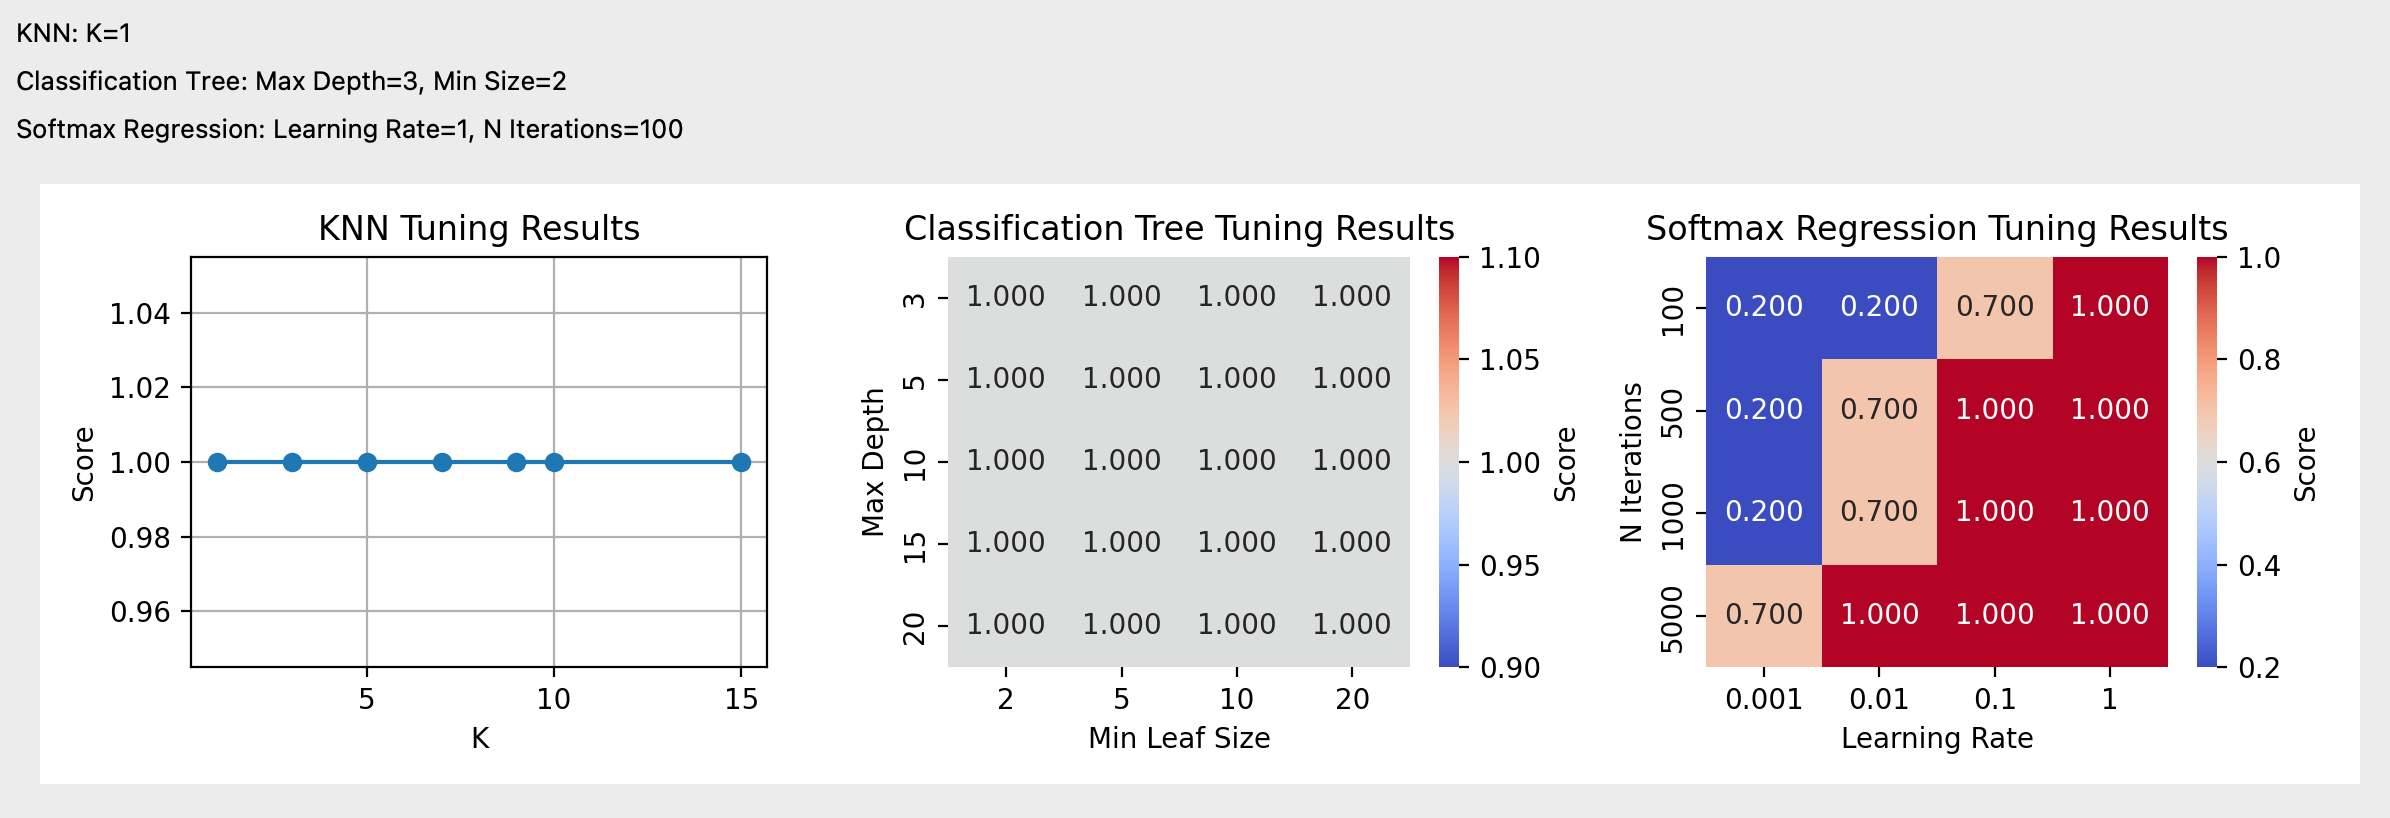
\includegraphics[width=1.0\textwidth]{iris_tuned.png}
    \caption{Iris Tuned Models}
    \label{iris_tuned}
\end{figure}

\begin{table}[ht]
\centering
\caption{Best hyperparameters for each model on the Iris dataset}
\label{tab:iris_tuning}
\begin{tabular}{|l|l|}
\hline
\textbf{Model} & \textbf{Best Hyperparameters} \\ % Add \\ here
\hline
KNN & K = 1 \\ % Add \\ here
\hline
Classification Tree & Max Depth = 3, Min Depth = 2 \\ % Add \\ here
\hline
Softmax Regression & Learning Rate = 1, Iterations = 100 \\ % Add \\ here
\hline
\end{tabular}
\end{table}

\subsubsection{Model Evaluation}

We evaluated the tuned models using 5-fold cross-validation and obtained various performance metrics. The results are presented in Table \ref{tab:iris_metrics}.

\begin{figure}[ht]
    \centering
    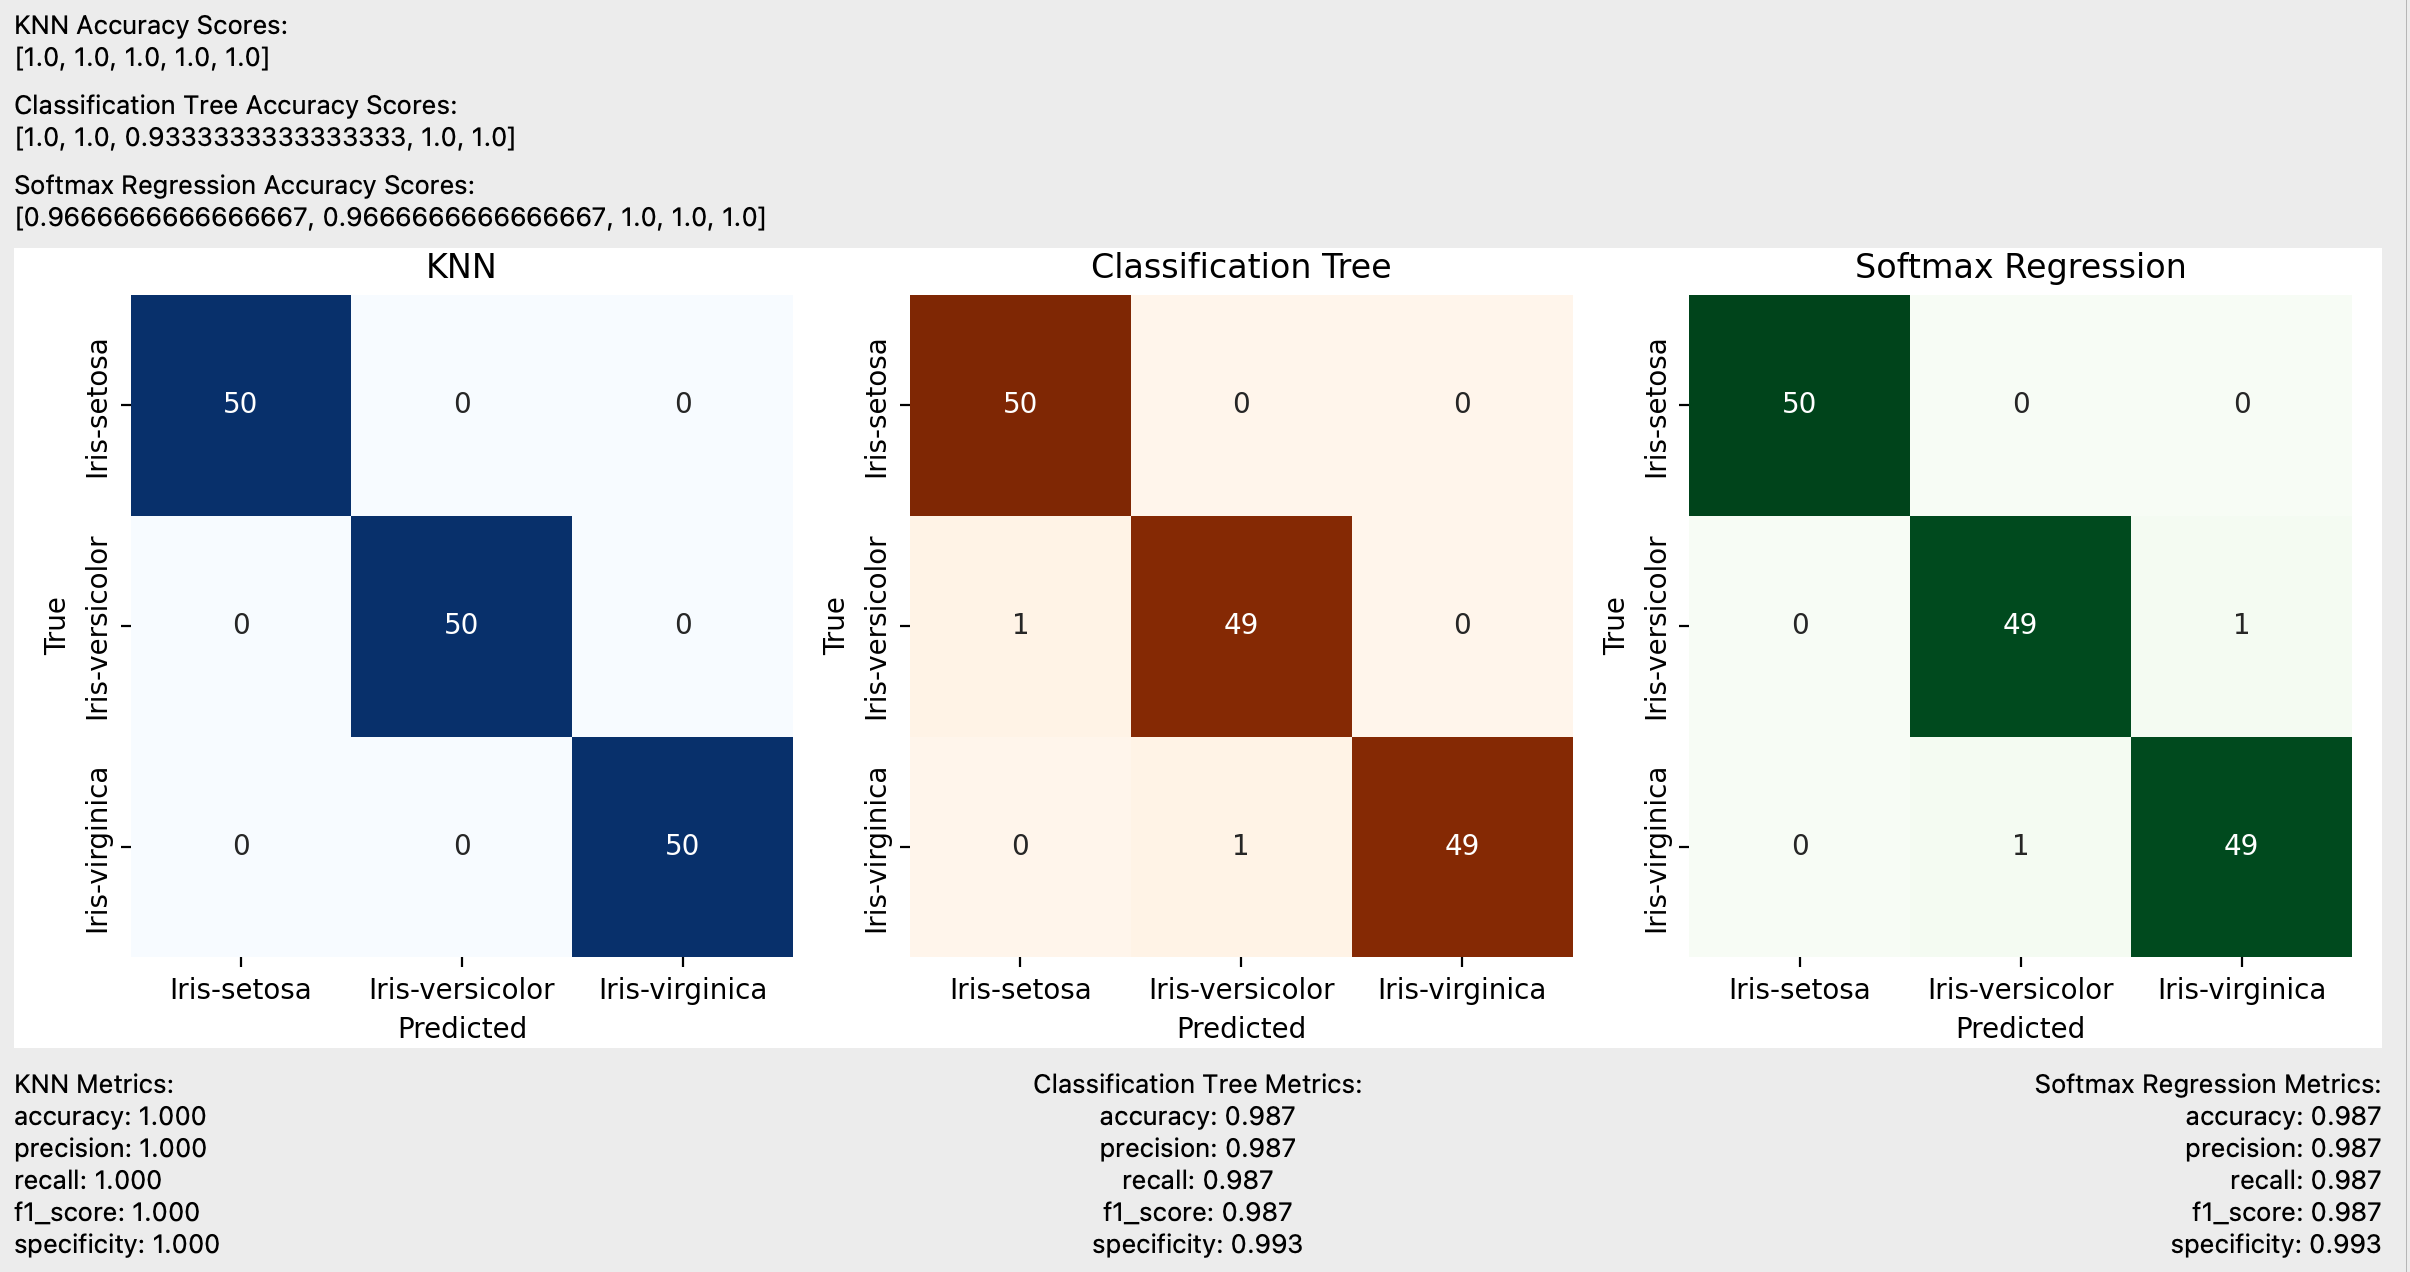
\includegraphics[width=1.0\textwidth]{iris_results.png}
    \caption{Iris Results}
    \label{iris_results}
\end{figure}

\begin{table}[ht]
\centering
\caption{Performance metrics for each model on the Iris dataset}
\label{tab:iris_metrics}
\begin{tabular}{|l|c|c|c|}
\hline
\textbf{Metric} & \textbf{KNN} & \textbf{Classification Tree} & \textbf{Softmax Regression} \\ % Add \\ here
\hline
Accuracy & 1.000 & 0.987 & 0.987 \\ % Add \\ here
\hline
Precision & 1.000 & 0.987 & 0.987 \\ % Add \\ here
\hline
Recall & 1.000 & 0.987 & 0.987 \\ % Add \\ here
\hline
F1-score & 1.000 & 0.987 & 0.987 \\ % Add \\ here
\hline
Specificity & 1.000 & 0.993 & 0.993 \\ % Add \\ here
\hline
\end{tabular}
\end{table}

\subsubsection{Observations}

Based on the performance metrics obtained from the 5-fold cross-validation, all three models demonstrate strong performance on the Iris dataset. The KNN model with K=1 achieves perfect scores across all metrics, indicating that it correctly classifies all instances in the dataset. However, it's important to note that setting K=1 may lead to overfitting, as the model becomes highly sensitive to individual data points and may not generalize well to unseen data. \par

The Classification Tree and Softmax Regression models also exhibit excellent performance, with accuracy, precision, recall, and F1-score of 0.987 and specificity of 0.993. These results suggest that both models effectively capture the underlying patterns in the Iris dataset and make accurate predictions. \par

Given the small size and simplicity of the Iris dataset, it is not surprising that all three models perform well. However, it is essential to evaluate their performance on larger and more complex datasets to gain deeper insights into their strengths, weaknesses, and generalization abilities. \par

\subsection{Ionosphere Dataset}

The Ionosphere~\cite{ionosphere} dataset is a binary classification dataset that contains radar data collected by a system in Goose Bay, Labrador, Canada. It consists of 351 instances, each with 34 continuous attributes representing various characteristics of the radar signals. The goal is to predict whether a given set of radar readings represents a "Good" or "Bad" radar return, indicating the presence or absence of structure in the ionosphere. \\par

Compared to the Iris dataset, the Ionosphere dataset is more complex due to its higher dimensionality (34 features) and the nature of the radar data. It provides an opportunity to evaluate the performance of machine learning algorithms on a real-world classification task involving signal processing and pattern recognition. \\par

\subsubsection{Model Tuning}

To optimize the performance of the models on the Ionosphere dataset, we conducted a model tuning process. The best hyperparameters for each model are presented in Table \ref{tab:ionosphere_tuning}.

\begin{figure}[ht]
    \centering
    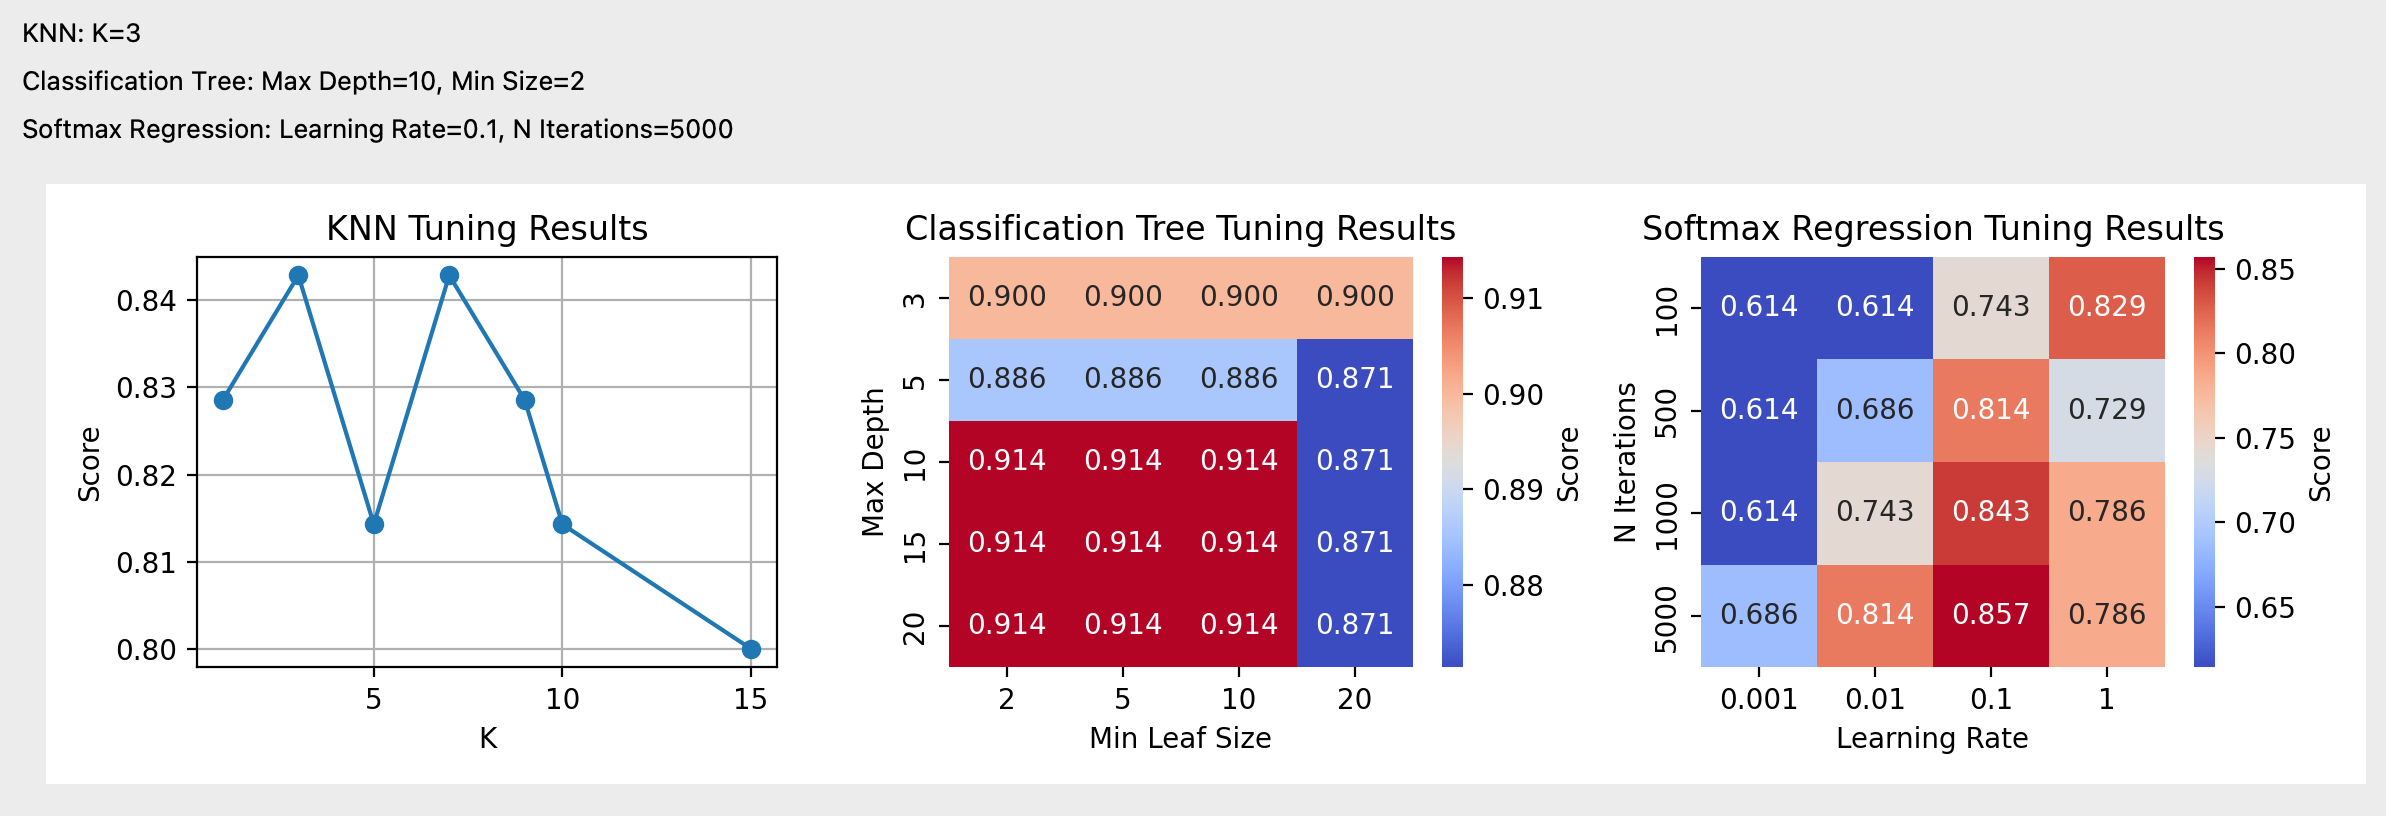
\includegraphics[width=1.0\textwidth]{iono_tuned.png}
    \caption{Ionosphere Tuned Models}
    \label{iono_tuned}
\end{figure}

\begin{table}[ht]
\centering
\caption{Best hyperparameters for each model on the Ionosphere dataset}
\label{tab:ionosphere_tuning}
\begin{tabular}{|l|l|}
\hline
\textbf{Model} & \textbf{Best Hyperparameters} \\
\hline
KNN & K = 3 \\
\hline
Classification Tree & Max Depth = 10, Min Size = 2 \\
\hline
Softmax Regression & Learning Rate = 0.1, Iterations = 5000 \\
\hline
\end{tabular}
\end{table}

\subsubsection{Model Evaluation}

We evaluated the tuned models using 5-fold cross-validation and obtained various performance metrics. The results are presented in Table \ref{tab:ionosphere_metrics}.

\begin{figure}[ht]
    \centering
    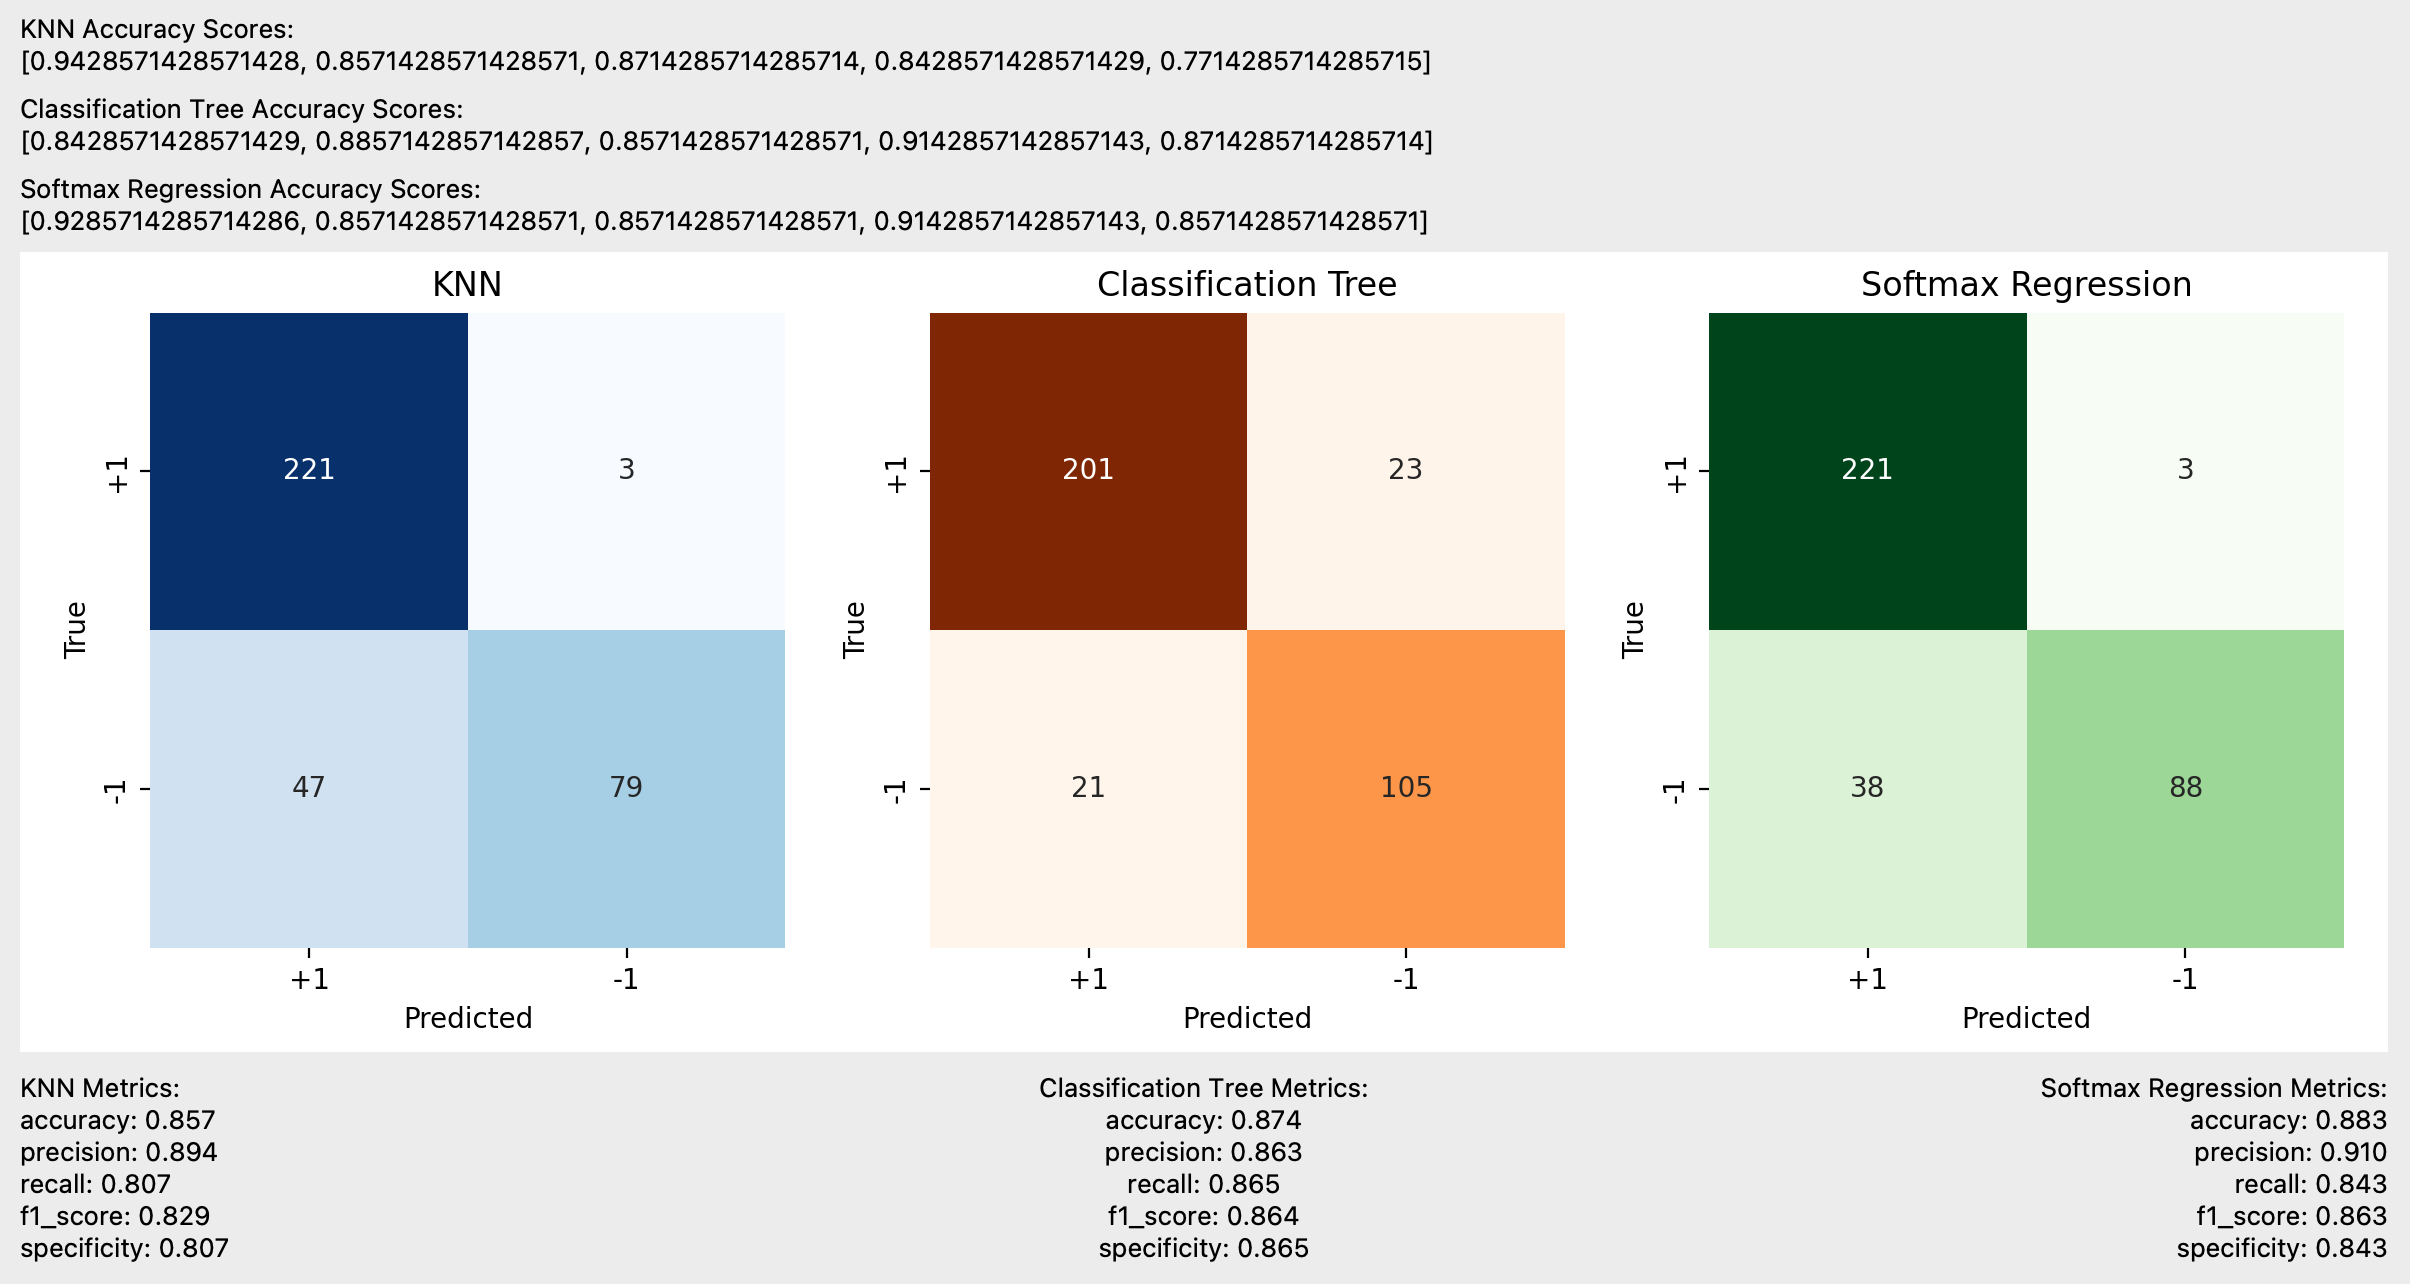
\includegraphics[width=1.0\textwidth]{iono_results.png}
    \caption{Ionosphere Results}
    \label{iono_results}
\end{figure}

\begin{table}[ht]
\centering
\caption{Performance metrics for each model on the Ionosphere dataset}
\label{tab:ionosphere_metrics}
\begin{tabular}{|l|c|c|c|}
\hline
\textbf{Metric} & \textbf{KNN} & \textbf{Classification Tree} & \textbf{Softmax Regression} \\
\hline
Accuracy & 0.857 & 0.874 & 0.883 \\
\hline
Precision & 0.894 & 0.863 & 0.910 \\
\hline
Recall & 0.807 & 0.865 & 0.843 \\
\hline
F1-score & 0.829 & 0.864 & 0.863 \\
\hline
Specificity & 0.807 & 0.865 & 0.843 \\
\hline
\end{tabular}
\end{table}

\subsubsection{Observations}

Based on the performance metrics, all three models demonstrate good performance on the Ionosphere dataset. The Softmax Regression model achieves the highest accuracy of 0.883 and precision of 0.910, indicating its effectiveness in capturing the decision boundary between the "Good" and "Bad" classes. The Classification Tree model closely follows with an accuracy of 0.874 and balanced recall and specificity scores of 0.865. The KNN model, while still performing well, has slightly lower scores compared to the other two models.\par

Looking at the accuracy scores within each fold (provided in the screenshot), we observe some variations across the folds for each model, suggesting the presence of bias and variance. However, the variations are not extremely large, indicating relatively stable models.\par


The results suggest that Softmax Regression and Classification Tree are particularly well-suited for this dataset, with KNN also providing decent performance.\par

\subsection{Titanic Dataset}

The Titanic~\cite{titanic} dataset is a well-known dataset in machine learning that contains information about passengers on the Titanic, the infamous ship that sank in the North Atlantic Ocean in 1912. The dataset consists of 891 instances, each representing a passenger on the ship. The goal is to predict whether a passenger survived or not based on various features such as age, gender, passenger class, and fare.

The Titanic dataset presents a binary classification problem with a mix of categorical and numerical features. It provides an opportunity to evaluate the performance of machine learning algorithms on a real-world dataset with historical significance and to explore the factors that influenced passenger survival.

\subsubsection{Model Tuning}

To optimize the performance of the models on the Titanic dataset, we conducted a model tuning process. The best hyperparameters for each model are presented in Table \ref{tab:titanic_tuning}.

\begin{figure}[ht]
    \centering
    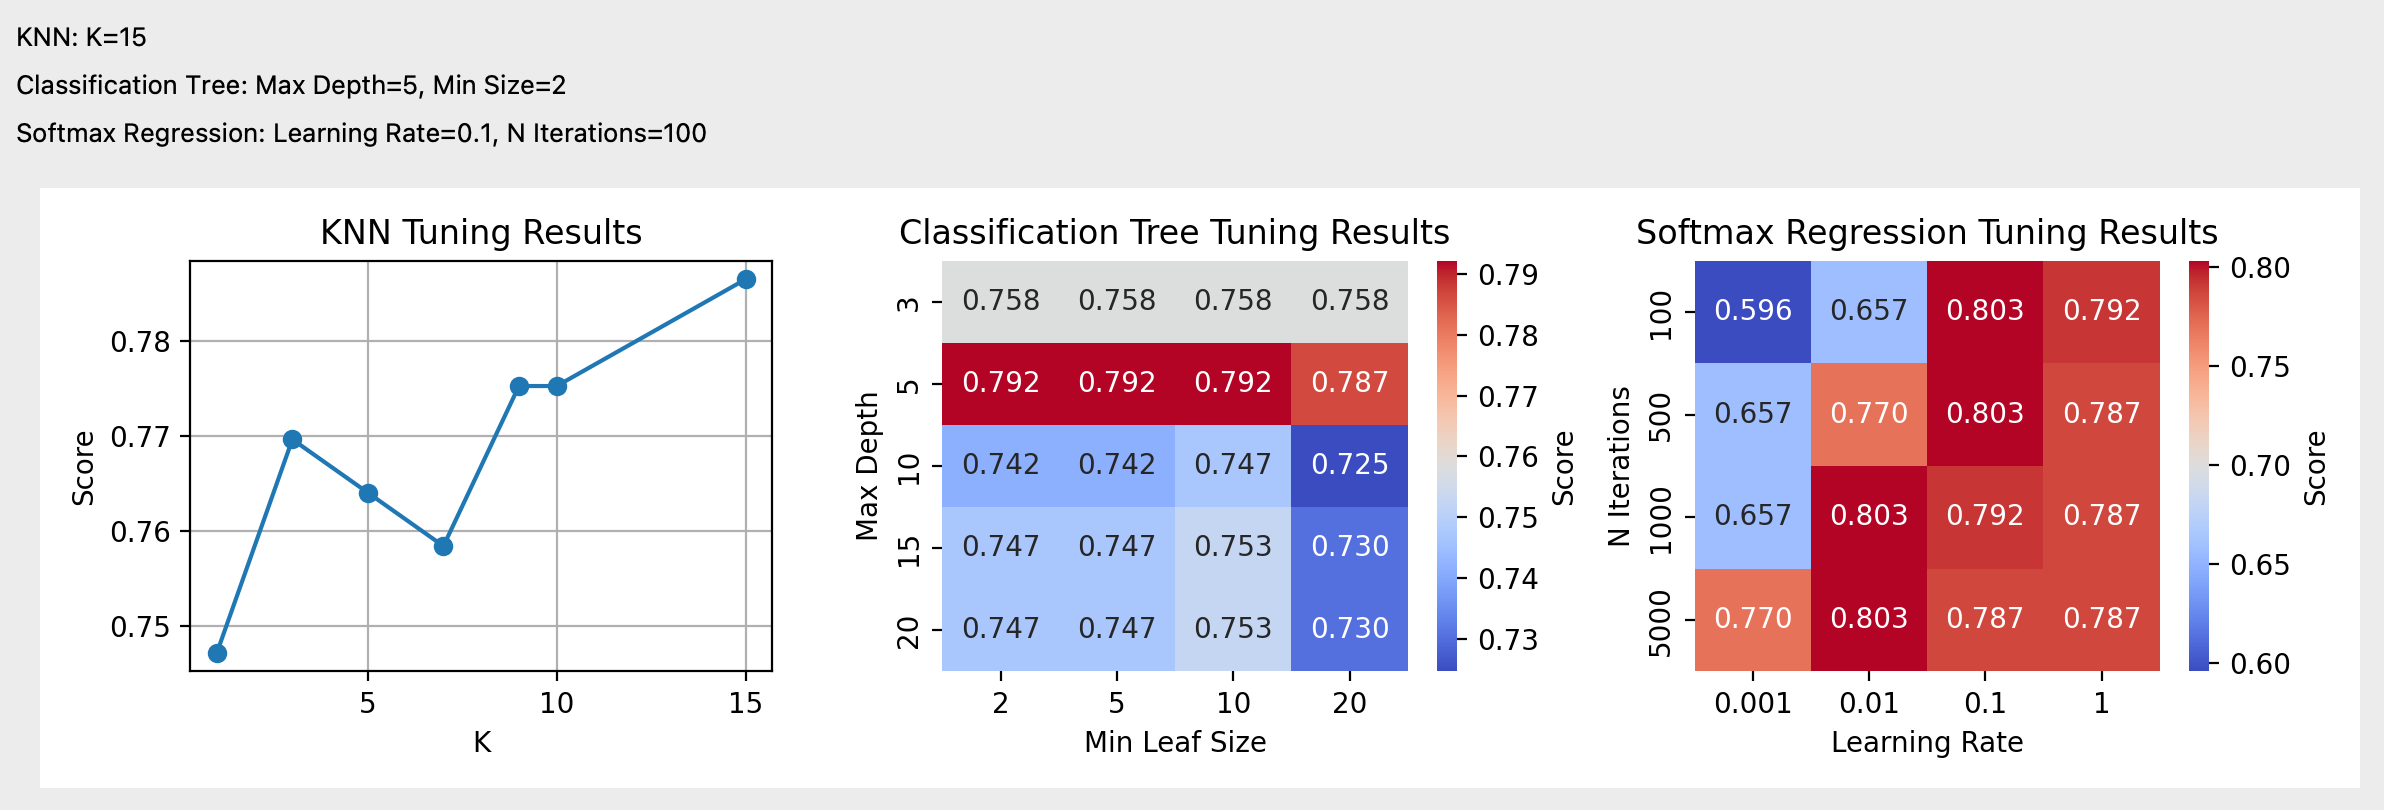
\includegraphics[width=1.0\textwidth]{titanic_tuned.png}
    \caption{Titanic Tuned Models}
    \label{titanic_tuned}
\end{figure}

\begin{table}[ht]
\centering
\caption{Best hyperparameters for each model on the Titanic dataset}
\label{tab:titanic_tuning}
\begin{tabular}{|l|l|}
\hline
\textbf{Model} & \textbf{Best Hyperparameters} \\
\hline
KNN & K = 15 \\
\hline
Classification Tree & Max Depth = 5, Min Size = 2 \\
\hline
Softmax Regression & Learning Rate = 0.1, Iterations = 100 \\
\hline
\end{tabular}
\end{table}

\subsubsection{Model Evaluation}

We evaluated the tuned models using 5-fold cross-validation and obtained various performance metrics. The results are presented in Table \ref{tab:titanic_metrics}.

\begin{figure}[ht]
    \centering
    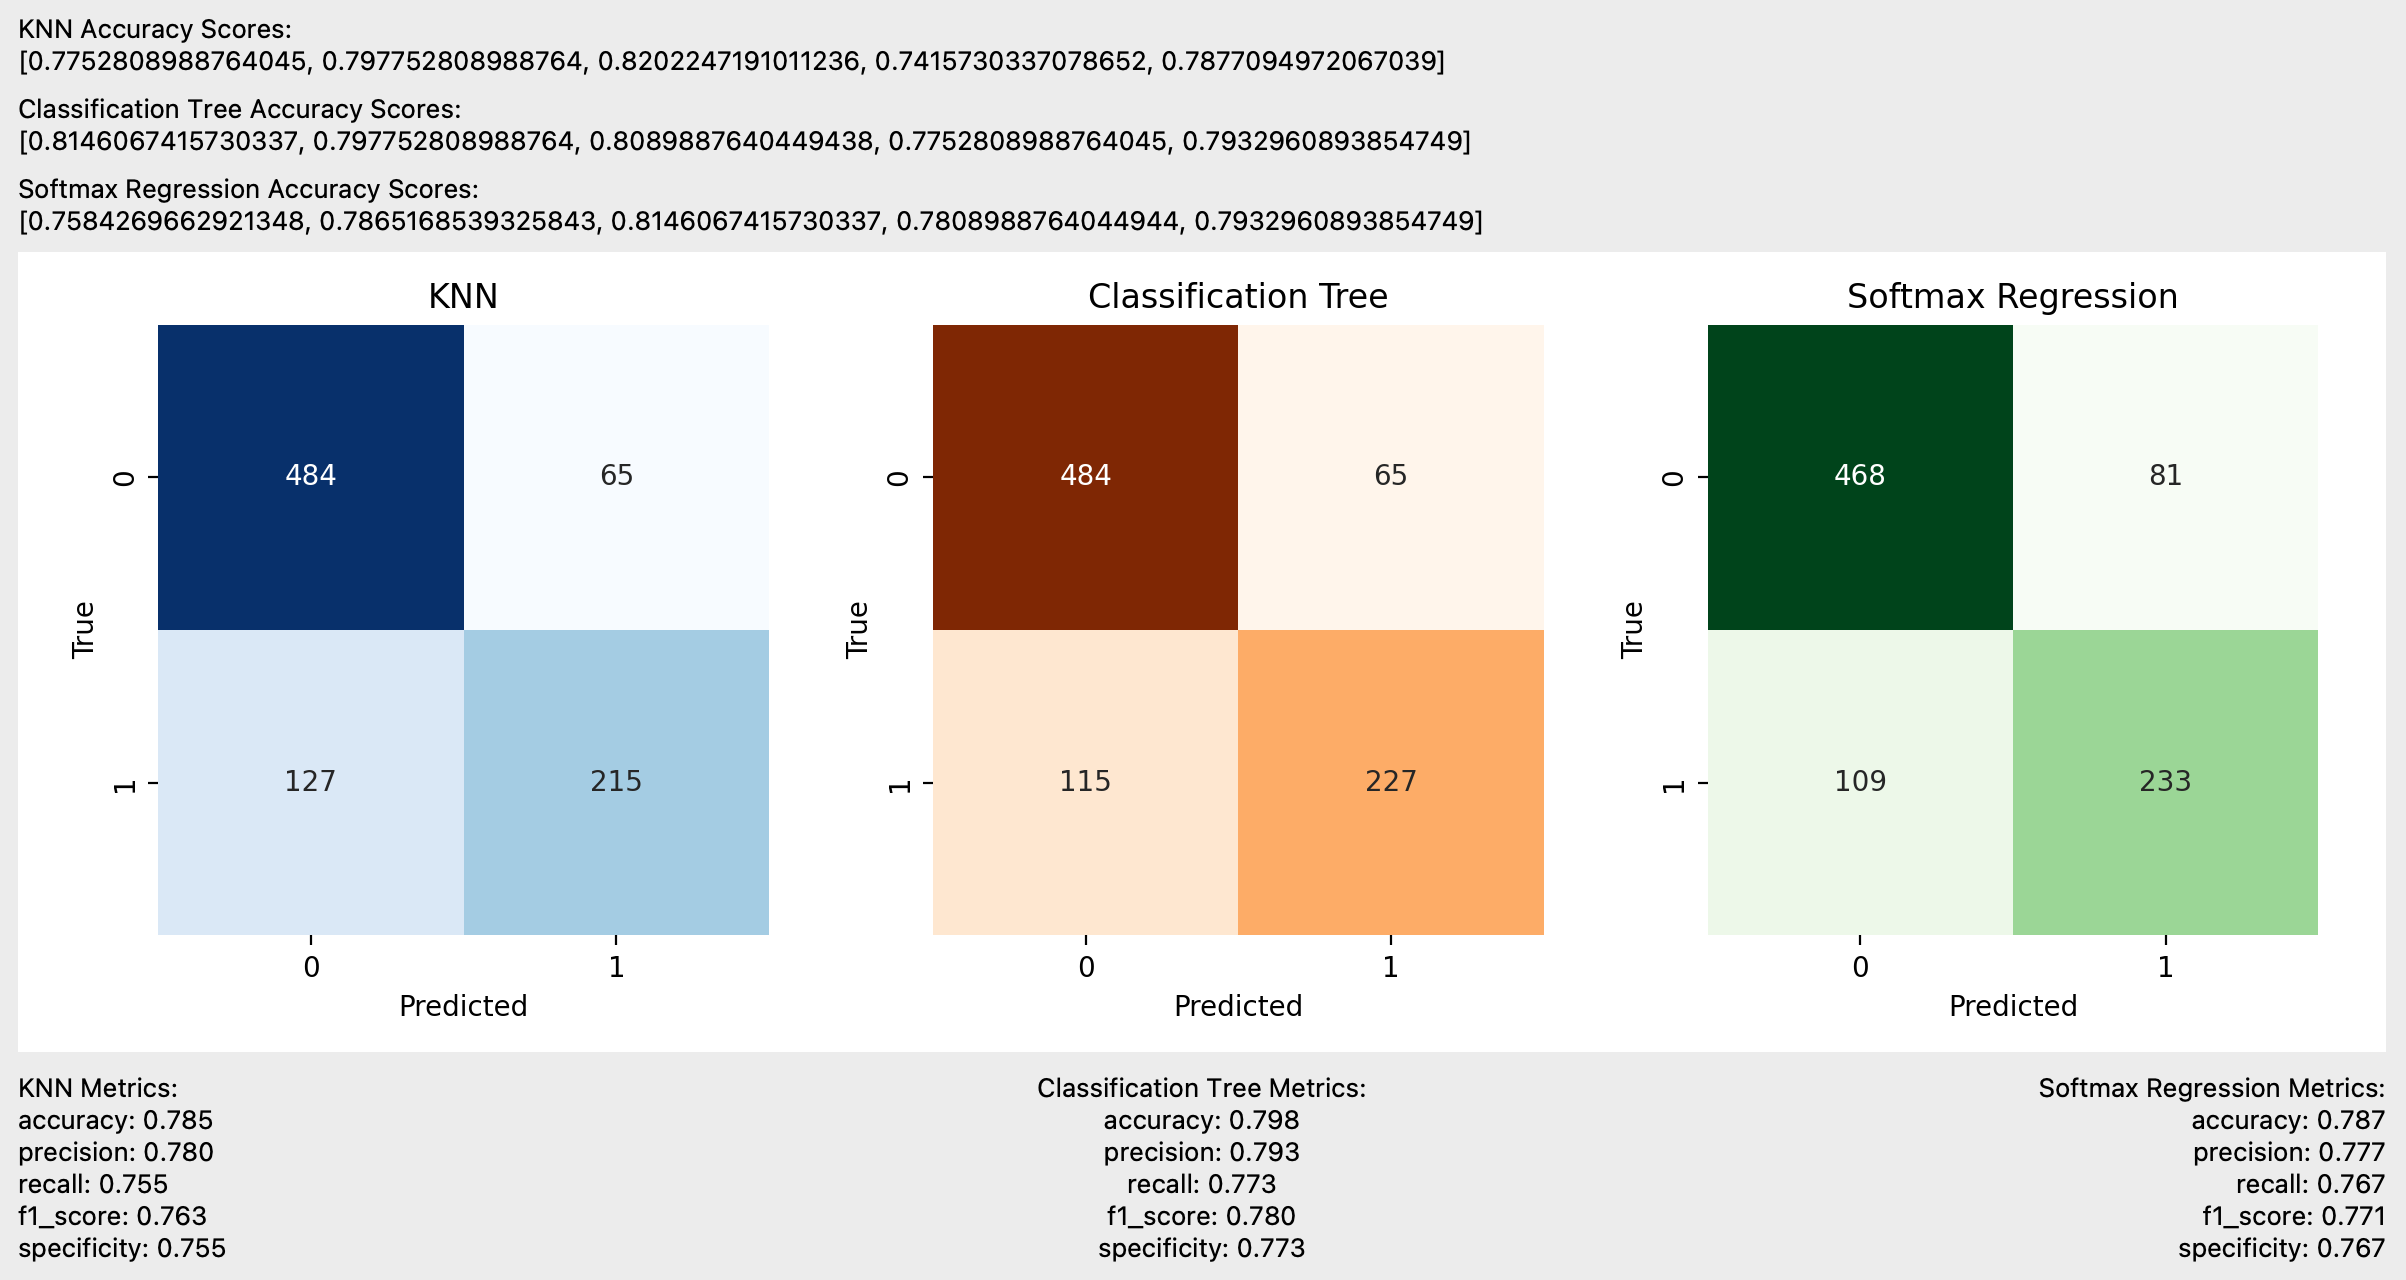
\includegraphics[width=1.0\textwidth]{titanic_results.png}
    \caption{Titanic Results}
    \label{titanic_results}
\end{figure}
\begin{table}[ht]
\centering
\caption{Performance metrics for each model on the Titanic dataset}
\label{tab:titanic_metrics}
\begin{tabular}{|l|c|c|c|}
\hline
\textbf{Metric} & \textbf{KNN} & \textbf{Classification Tree} & \textbf{Softmax Regression} \\
\hline
Accuracy & 0.785 & 0.798 & 0.787 \\
\hline
Precision & 0.780 & 0.793 & 0.777 \\
\hline
Recall & 0.755 & 0.773 & 0.767 \\
\hline
F1-score & 0.763 & 0.780 & 0.771 \\
\hline
Specificity & 0.755 & 0.773 & 0.767 \\
\hline
\end{tabular}
\end{table}


\subsubsection{Observations}

Based on the performance metrics, the Classification Tree model achieves the highest accuracy of 0.798 on the Titanic dataset, closely followed by Softmax Regression with an accuracy of 0.787 and KNN with an accuracy of 0.785. The Classification Tree model also demonstrates the highest precision, recall, F1-score, and specificity among the three models.\par

The results suggest that the Classification Tree model is particularly well-suited for the Titanic dataset, likely due to its ability to capture complex relationships and handle the mix of categorical and numerical features. Softmax Regression and KNN also provide comparable performance, with Softmax Regression slightly outperforming KNN. \par

Looking at the accuracy scores within each fold (provided in the screenshot), we observe some variations across the folds for each model, indicating the presence of bias and variance. The variations are relatively small, suggesting that the models are fairly stable and generalize well to unseen data. \par

It's worth noting that the performance metrics for all models are lower compared to the previous datasets (Iris and Ionosphere). This suggests that the Titanic dataset presents a more challenging classification task, possibly due to the complex interplay of factors influencing passenger survival and the presence of missing values. \par

This dataset was also the first test for our application at handling multivariate data as well as missing data, which it seemed to handle smoothly. \par

Overall, the Titanic dataset provides a realistic scenario to evaluate the performance of machine learning models and highlights the importance of data preprocessing and feature engineering in achieving better results.

\subsection{Car Evaluation Dataset}

The Car Evaluation dataset~\cite{misc_car_evaluation_19} is a classic dataset used for classification tasks in machine learning. It contains information about various car models and their characteristics, such as price, maintenance cost, number of doors, capacity, luggage boot size, and safety. The goal is to classify the cars into four categories: unacceptable, acceptable, good, and very good, based on these features.

The dataset consists of 1,728 instances, each representing a car model. It includes a mix of categorical and numerical features, making it suitable for evaluating the performance of different classification algorithms and exploring the relationship between car attributes and their overall acceptability.

\subsubsection{Model Tuning}

To optimize the performance of the models on the Car Evaluation dataset, we conducted a model tuning process. The best hyperparameters for each model are presented in Table \ref{tab:car_tuning}.

\begin{figure}[ht]
    \centering
    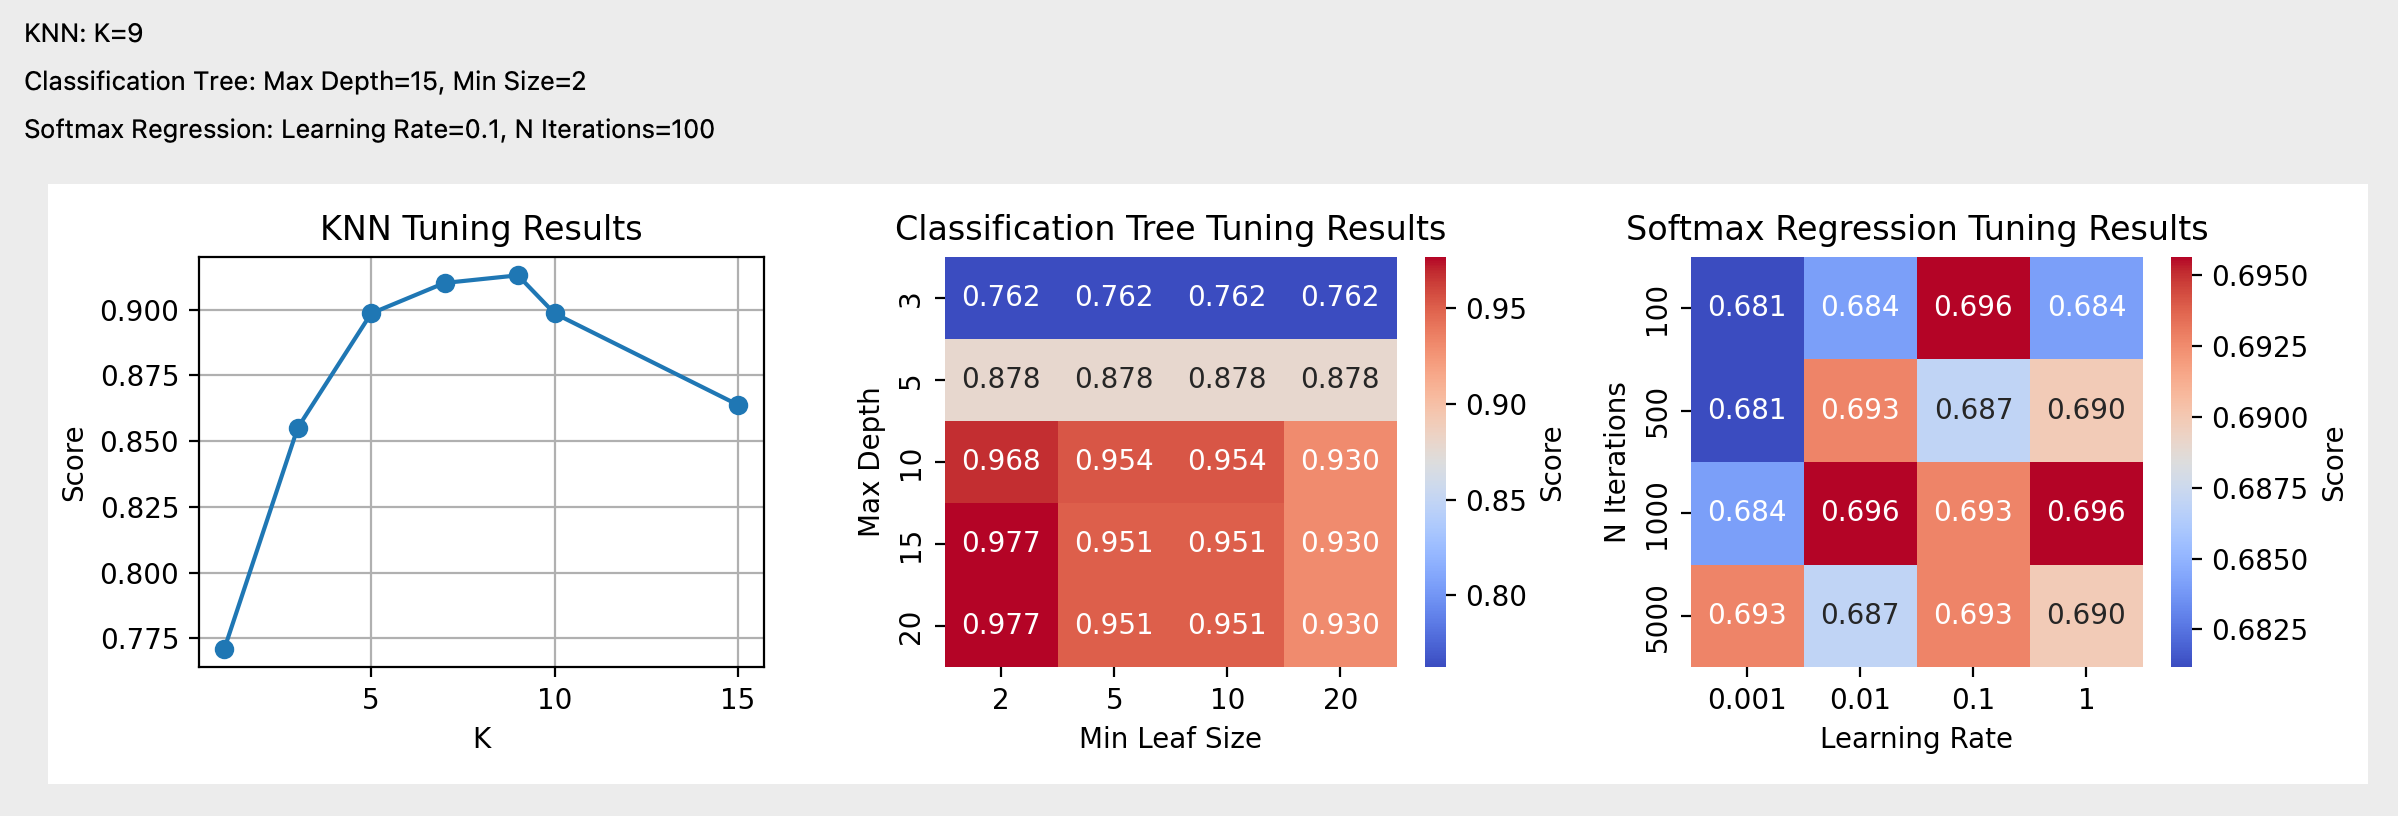
\includegraphics[width=1.0\textwidth]{car_eval_tuned.png}
    \caption{Car Evaluation Tuned Models}
    \label{car_eval_tuned}
\end{figure}

\begin{table}[ht]
\centering
\caption{Best hyperparameters for each model on the Car Evaluation dataset}
\label{tab:car_tuning}
\begin{tabular}{|l|l|}
\hline
\textbf{Model} & \textbf{Best Hyperparameters} \\
\hline
KNN & K = 9 \\
\hline
Classification Tree & Max Depth = 15, Min Size = 2 \\
\hline
Softmax Regression & Learning Rate = 0.1, Iterations = 100 \\
\hline
\end{tabular}
\end{table}


\subsubsection{Model Evaluation}

We evaluated the tuned models using 5-fold cross-validation and obtained various performance metrics. The results are presented in Table \ref{tab:car_metrics}.

\begin{figure}[ht]
    \centering
    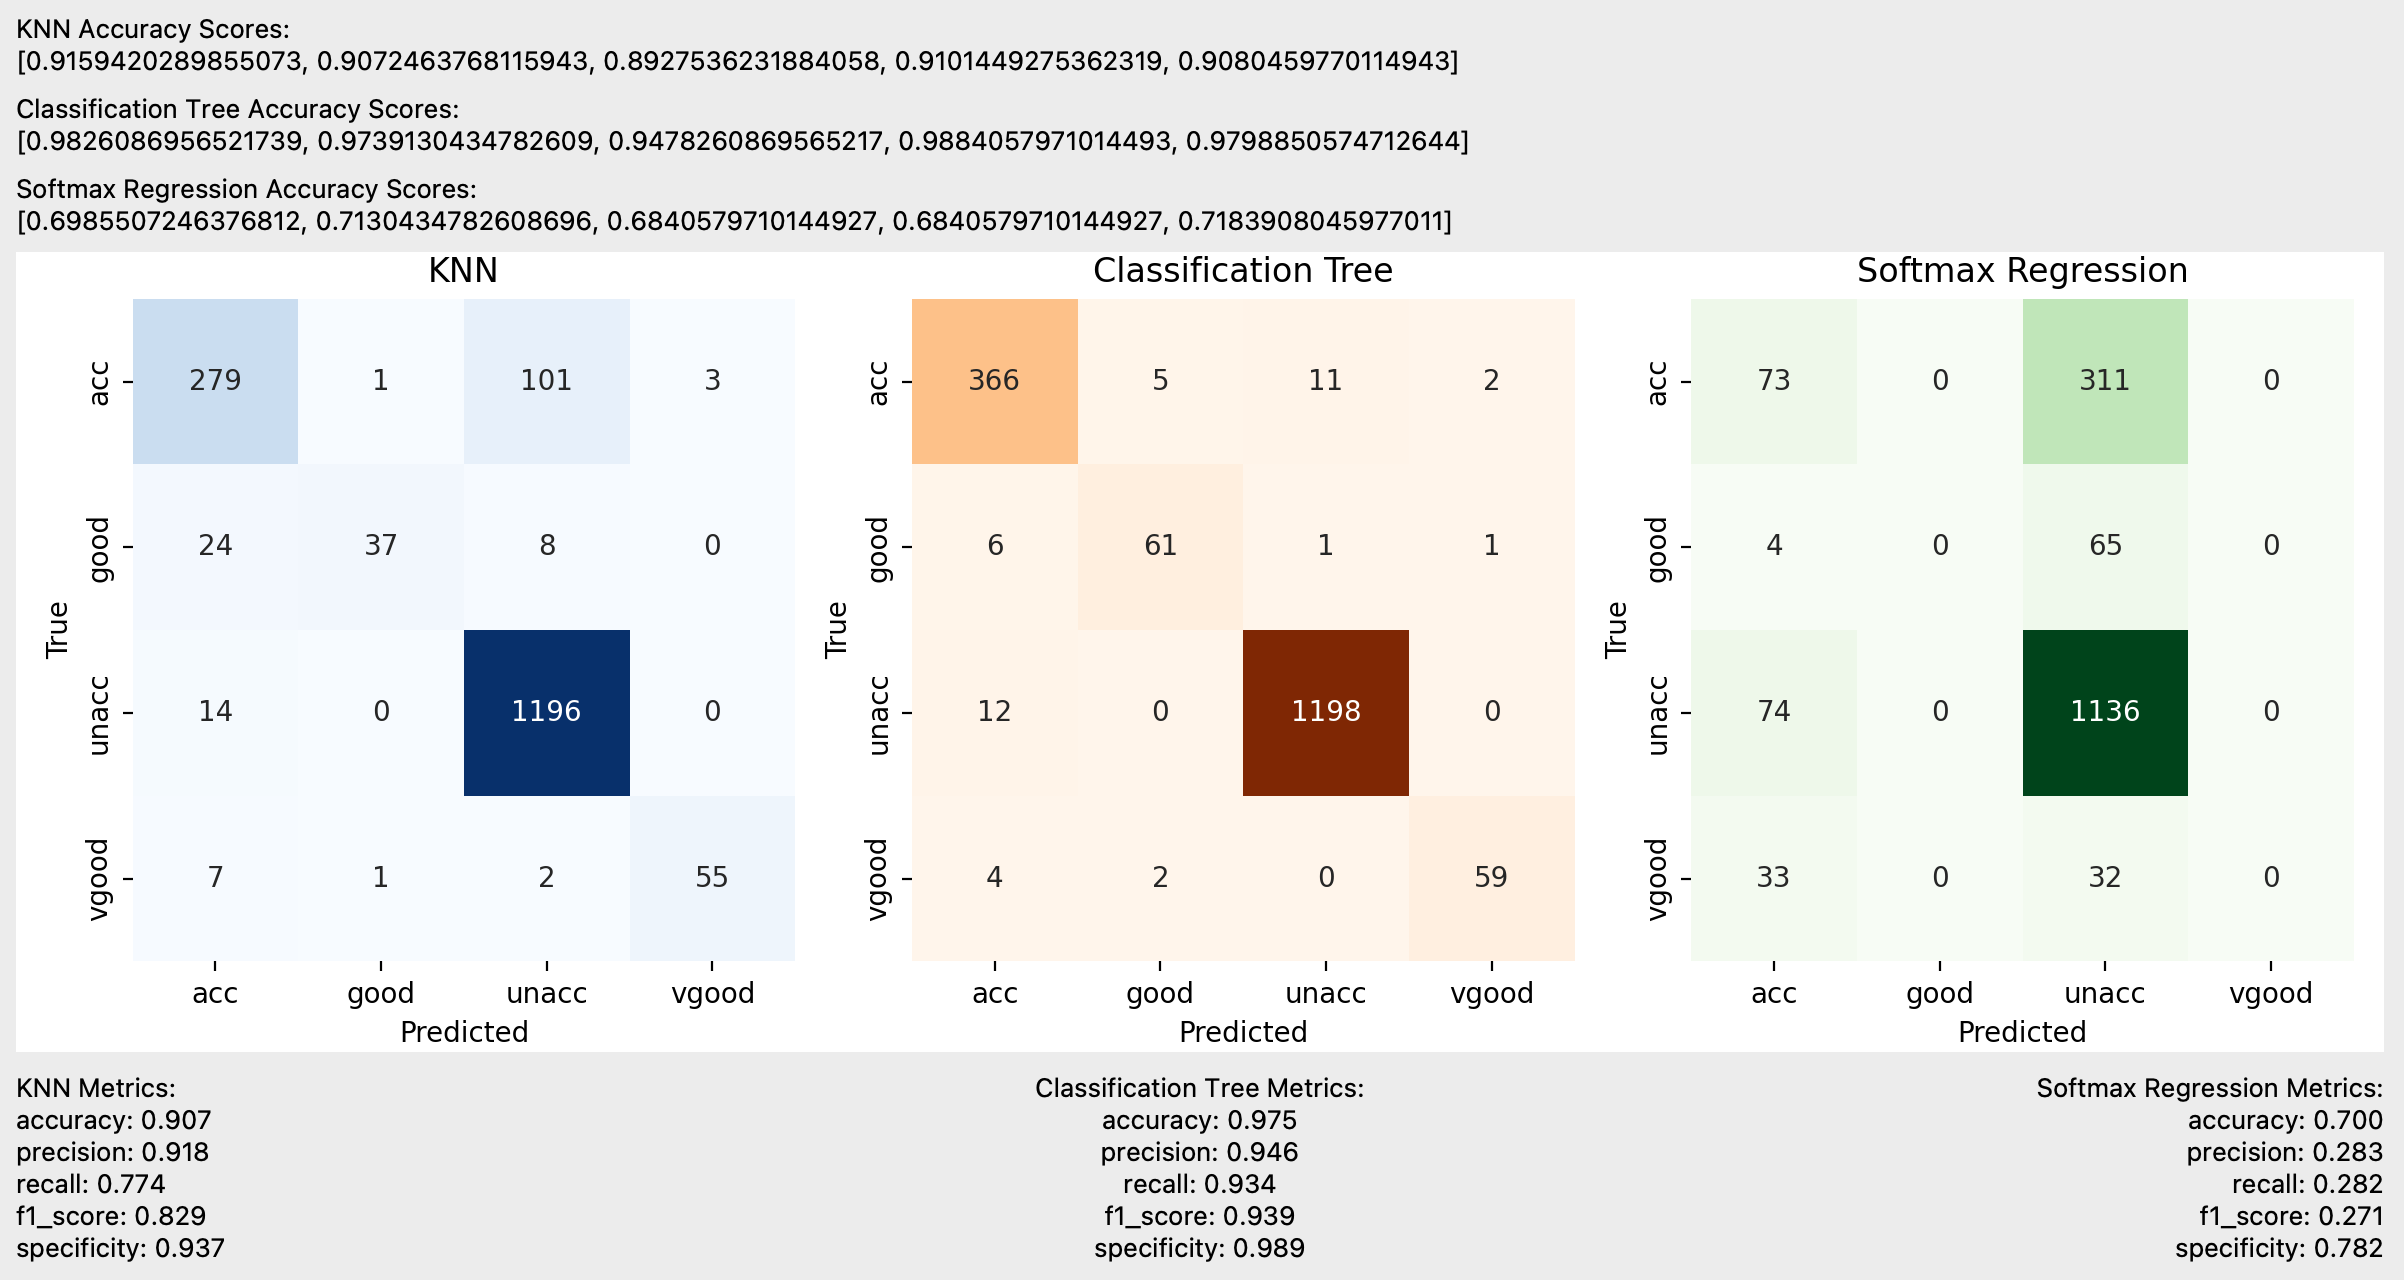
\includegraphics[width=1.0\textwidth]{car_eval_results.png}
    \caption{Car Evaluation Results}
    \label{car_eval_results}
\end{figure}

\begin{table}[ht]
\centering
\caption{Performance metrics for each model on the Car Evaluation dataset}
\label{tab:car_metrics}
\begin{tabular}{|l|c|c|c|}
\hline
\textbf{Metric} & \textbf{KNN} & \textbf{Classification Tree} & \textbf{Softmax Regression} \\
\hline
Accuracy & 0.907 & 0.975 & 0.700 \\
\hline
Precision & 0.918 & 0.946 & 0.283 \\
\hline
Recall & 0.774 & 0.934 & 0.282 \\
\hline
F1-score & 0.829 & 0.939 & 0.271 \\
\hline
Specificity & 0.937 & 0.989 & 0.782 \\
\hline
\end{tabular}
\end{table}


\subsubsection{Observations}

Based on the performance metrics, the Classification Tree model achieves outstanding results on the Car Evaluation dataset, with an accuracy of 0.975, precision of 0.946, recall of 0.934, F1-score of 0.939, and specificity of 0.989. It significantly outperforms the other two models, indicating its strong ability to capture the underlying patterns and make accurate predictions.

The KNN model also performs well, with an accuracy of 0.907, precision of 0.918, and specificity of 0.937. However, its recall and F1-score are lower compared to the Classification Tree model, suggesting that it may have some limitations in correctly identifying certain car categories.

On the other hand, the Softmax Regression model shows relatively poor performance on this dataset, with an accuracy of 0.700, precision of 0.283, recall of 0.282, and F1-score of 0.271. This indicates that the linear nature of Softmax Regression may not be well-suited for capturing the complex relationships between the car features and their acceptability ratings.

Looking at the accuracy scores within each fold (provided in the screenshot), we observe relatively consistent performance across the folds for the Classification Tree and KNN models, suggesting good generalization ability. However, the Softmax Regression model shows more variability, indicating potential issues with bias and variance.

To further improve the performance, especially for the Softmax Regression model, we can consider the following:

\begin{itemize}
    \item \textbf{Feature engineering:} Creating new features or transforming existing ones to better capture the underlying patterns.
    \item \textbf{Regularization techniques:} Applying regularization methods such as L1 or L2 regularization to mitigate overfitting and improve generalization.
    \item \textbf{Ensemble methods:} Combining multiple models, such as decision trees or random forests, to leverage their collective predictive power.
\end{itemize}

Overall, the Car Evaluation dataset demonstrates the strength of the Classification Tree model in handling categorical features and making accurate predictions. It also highlights the importance of selecting appropriate algorithms based on the nature of the data and the problem at hand.

\subsection{Breast Cancer Wisconsin Dataset}

The Breast Cancer Wisconsin~\cite{breastcancerdataset_wisconsion} dataset is a widely used dataset in machine learning for binary classification tasks. It contains information about breast cancer patients, including various characteristics of the cell nuclei present in the digitized images of fine needle aspirate (FNA) of breast mass. The goal is to classify the breast cancer cases into two categories: malignant (cancerous) or benign (non-cancerous).

The dataset consists of 569 instances, each representing a patient. It includes 30 features computed from the cell nuclei, such as radius, texture, perimeter, area, smoothness, compactness, concavity, concave points, symmetry, and fractal dimension. These features are calculated from the digitized images and provide valuable information for distinguishing between malignant and benign tumors.

\subsubsection{Model Tuning}

To optimize the performance of the models on the Breast Cancer Wisconsin dataset, we conducted a model tuning process. The best hyperparameters for each model are presented in Table \ref{tab:breast_cancer_tuning}.
\begin{figure}[ht]
    \centering
    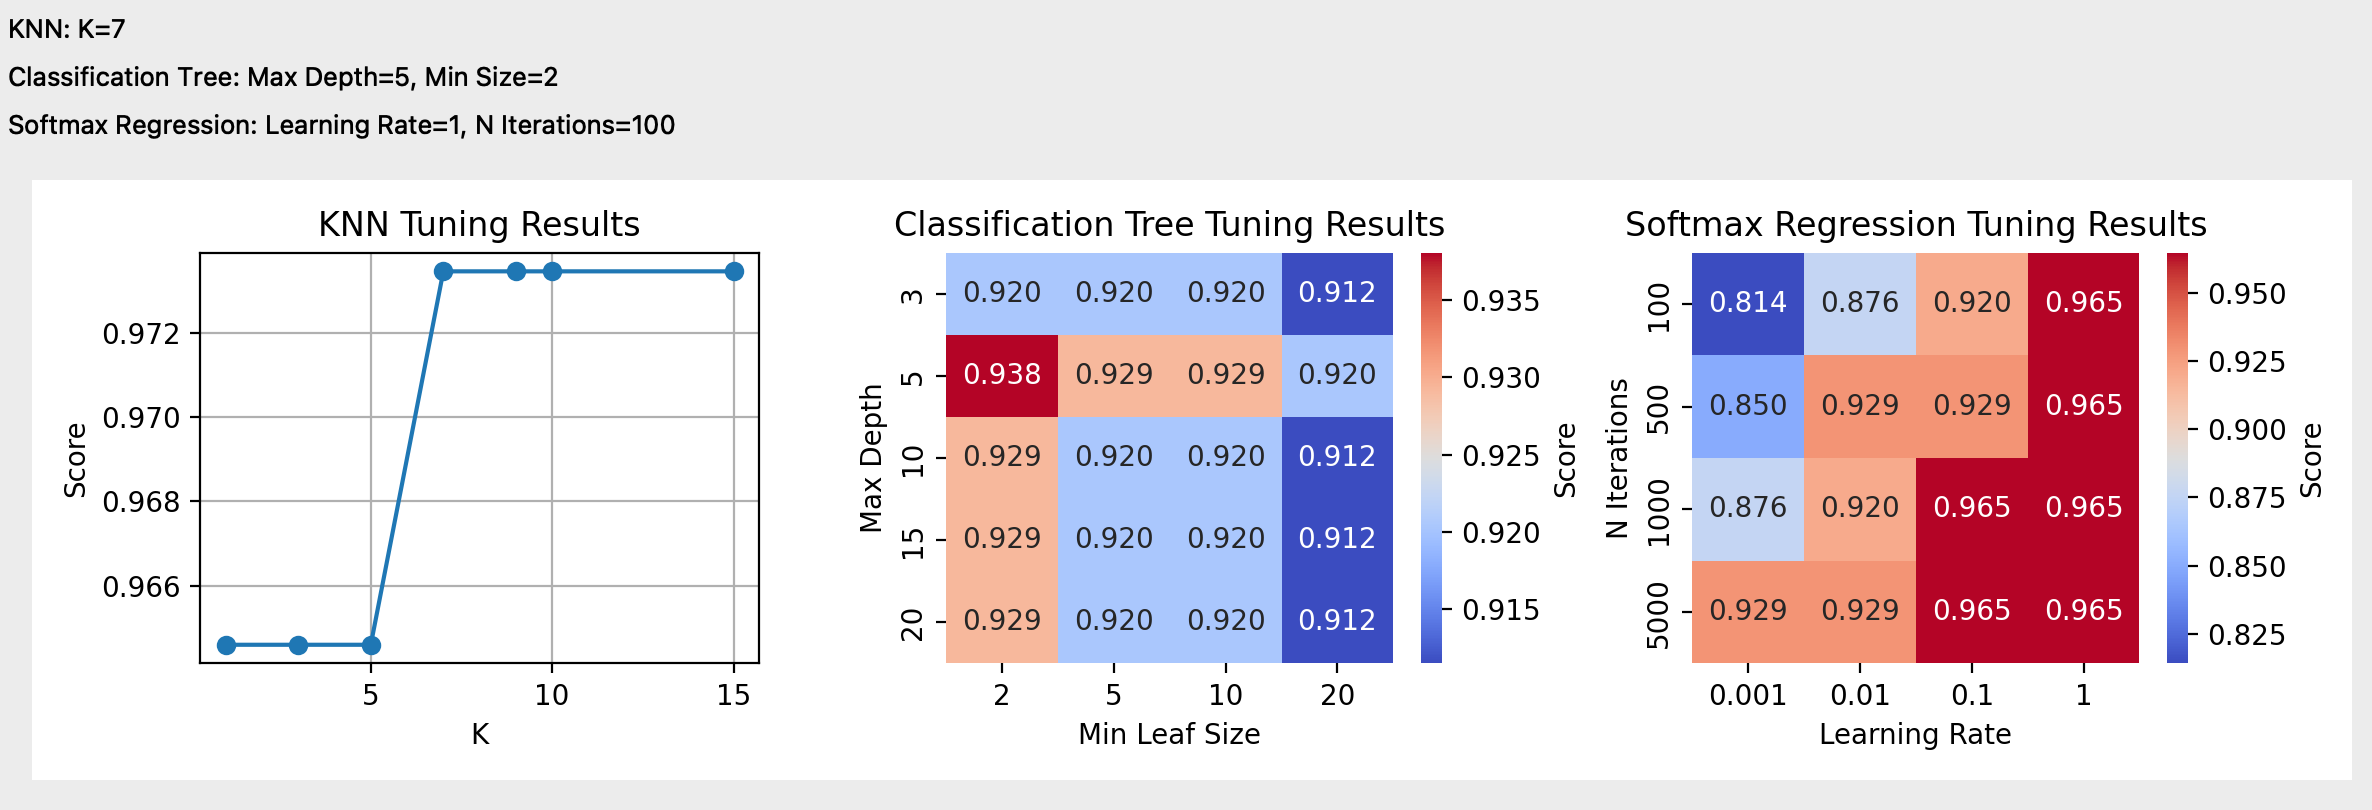
\includegraphics[width=1.0\textwidth]{bcancer_tuned.png}
    \caption{Breast Cancer Tuned Models}
    \label{bcancer_tuned}
\end{figure}
\begin{table}[h]
\centering
\caption{Best hyperparameters for each model on the Breast Cancer Wisconsin dataset}
\label{tab:breast_cancer_tuning}
\begin{tabular}{|l|l|}
\hline
\textbf{Model} & \textbf{Best Hyperparameters} \\
\hline
KNN & K = 7 \\
\hline
Classification Tree & Max Depth = 5, Min Size = 2 \\
\hline
Softmax Regression & Learning Rate = 1, Iterations = 100 \\
\hline
\end{tabular}
\end{table}

\subsubsection{Model Evaluation}

We evaluated the tuned models using 5-fold cross-validation and obtained various performance metrics. The results are presented in Table \ref{tab:breast_cancer_metrics}.

\begin{figure}[ht]
    \centering
    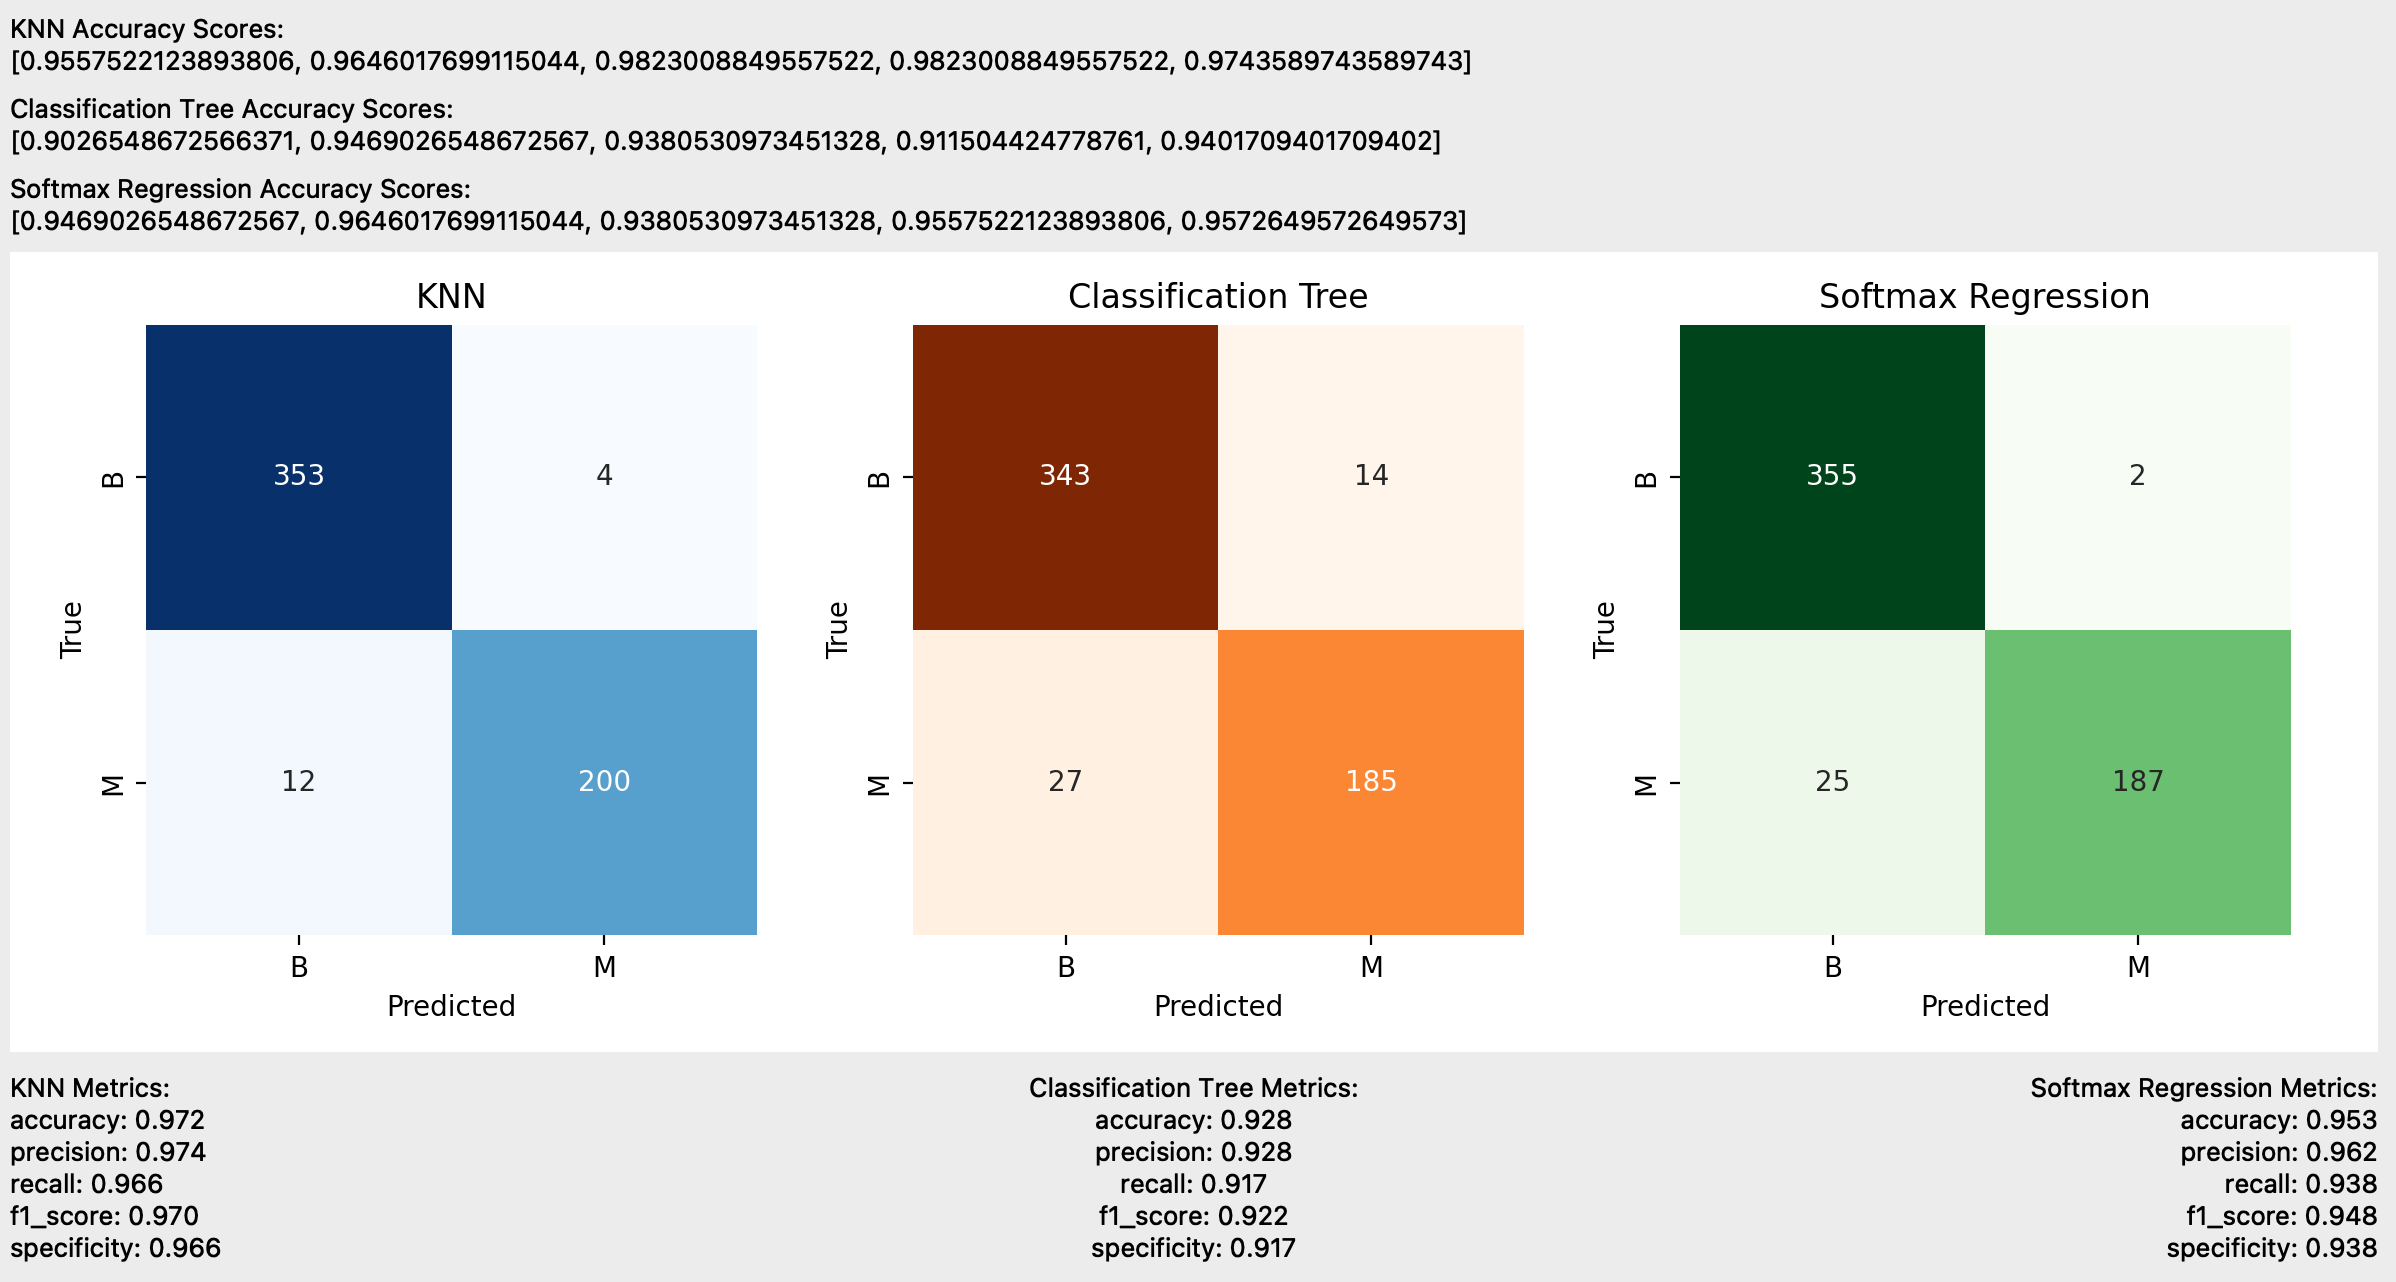
\includegraphics[width=1.0\textwidth]{bcancer_results.png}
    \caption{Breast Cancer Results}
    \label{bcancer_results}
\end{figure}
\begin{table}[h]
\centering
\caption{Performance metrics for each model on the Breast Cancer Wisconsin dataset}
\label{tab:breast_cancer_metrics}
\begin{tabular}{|l|c|c|c|}
\hline
\textbf{Metric} & \textbf{KNN} & \textbf{Classification Tree} & \textbf{Softmax Regression} \\
\hline
Accuracy & 0.972 & 0.928 & 0.953 \\
\hline
Precision & 0.974 & 0.928 & 0.962 \\
\hline
Recall & 0.966 & 0.917 & 0.938 \\
\hline
F1-score & 0.970 & 0.922 & 0.948 \\
\hline
Specificity & 0.966 & 0.917 & 0.938 \\
\hline
\end{tabular}
\end{table}


\subsubsection{Observations}

Based on the performance metrics, all three models demonstrate strong performance on the Breast Cancer Wisconsin dataset. The KNN model achieves the highest accuracy of 0.972, precision of 0.974, recall of 0.966, F1-score of 0.970, and specificity of 0.966. This indicates that the KNN model is highly effective in distinguishing between malignant and benign breast cancer cases.

The Softmax Regression model also performs well, with an accuracy of 0.953, precision of 0.962, recall of 0.938, F1-score of 0.948, and specificity of 0.938. This suggests that the linear nature of Softmax Regression is able to capture the discriminative patterns in the dataset and make accurate predictions.

The Classification Tree model, while still achieving good performance, has slightly lower metrics compared to KNN and Softmax Regression. It has an accuracy of 0.928, precision of 0.928, recall of 0.917, F1-score of 0.922, and specificity of 0.917. This may indicate that the tree-based approach may not be as effective as the other two models in capturing the complex relationships between the cell nuclei features and the cancer diagnosis.

Looking at the accuracy scores within each fold (provided in the screenshot), we observe relatively consistent performance across the folds for all three models, suggesting good generalization ability and robustness to variations in the data.

\subsection{Seeds Dataset}

The Seeds dataset~\cite{misc_seeds_236} is a commonly used dataset for classification tasks in machine learning. It contains measurements of geometrical properties of kernels belonging to three different varieties of wheat: Kama, Rosa, and Canadian. The goal is to classify the kernels into their respective wheat varieties based on these measured attributes.

The dataset consists of 210 instances, with 70 instances for each wheat variety. Each instance is characterized by seven attributes: area, perimeter, compactness, length of kernel, width of kernel, asymmetry coefficient, and length of kernel groove. These attributes capture various geometrical properties of the wheat kernels.

\subsubsection{Model Tuning}

To optimize the performance of the models on the Seeds dataset, we conducted a model tuning process. The best hyperparameters for each model are presented in Table \ref{tab:seeds_tuning}.

\begin{figure}[ht]
    \centering
    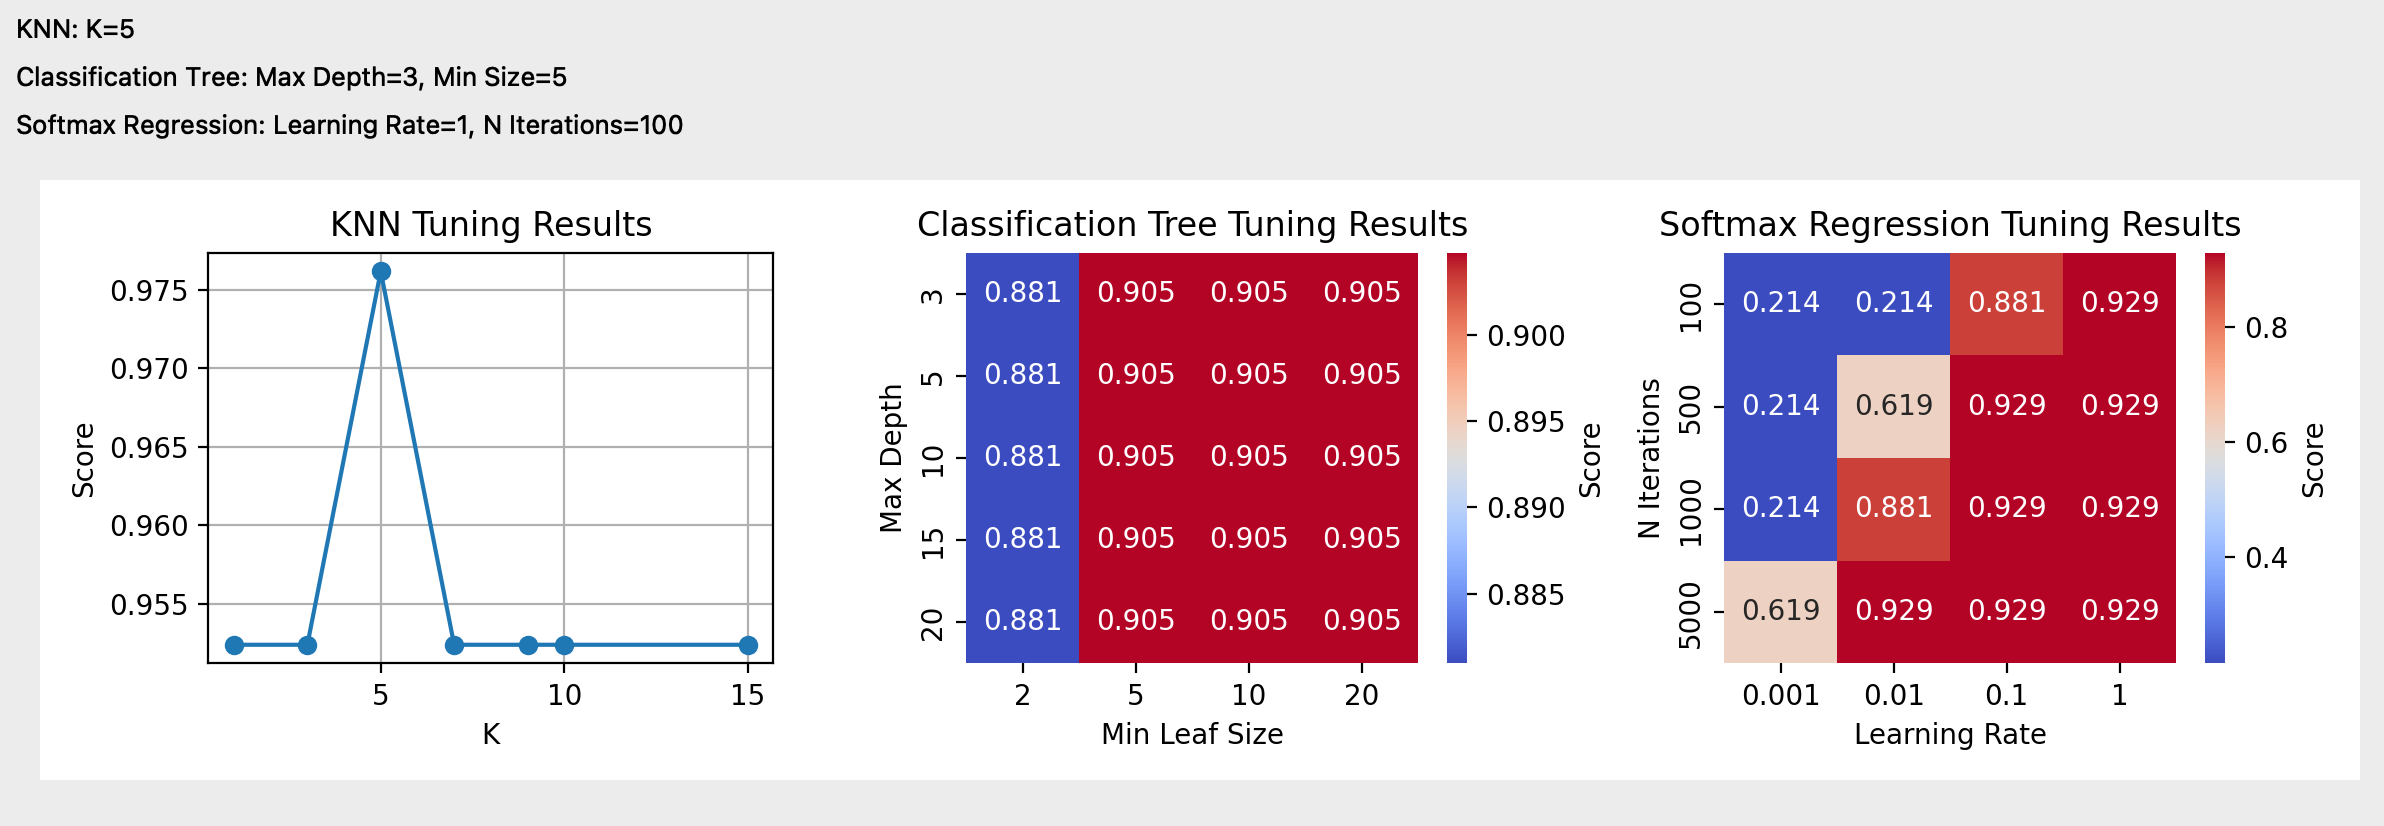
\includegraphics[width=1.0\textwidth]{seeds_tuned.png}
    \caption{Seeds Tuned Models}
    \label{seeds_tuned}
\end{figure}
\begin{table}[ht]
\centering
\caption{Best hyperparameters for each model on the Seeds dataset}
\label{tab:seeds_tuning}
\begin{tabular}{|l|l|}
\hline
\textbf{Model} & \textbf{Best Hyperparameters} \\
\hline
KNN & K = 5 \\
\hline
Classification Tree & Max Depth = 3, Min Size = 5 \\
\hline
Softmax Regression & Learning Rate = 1, Iterations = 100 \\
\hline
\end{tabular}
\end{table}

\subsubsection{Model Evaluation}

We evaluated the tuned models using 5-fold cross-validation and obtained various performance metrics. The results are presented in Table \ref{tab:seeds_metrics}.

\begin{figure}[ht]
    \centering
    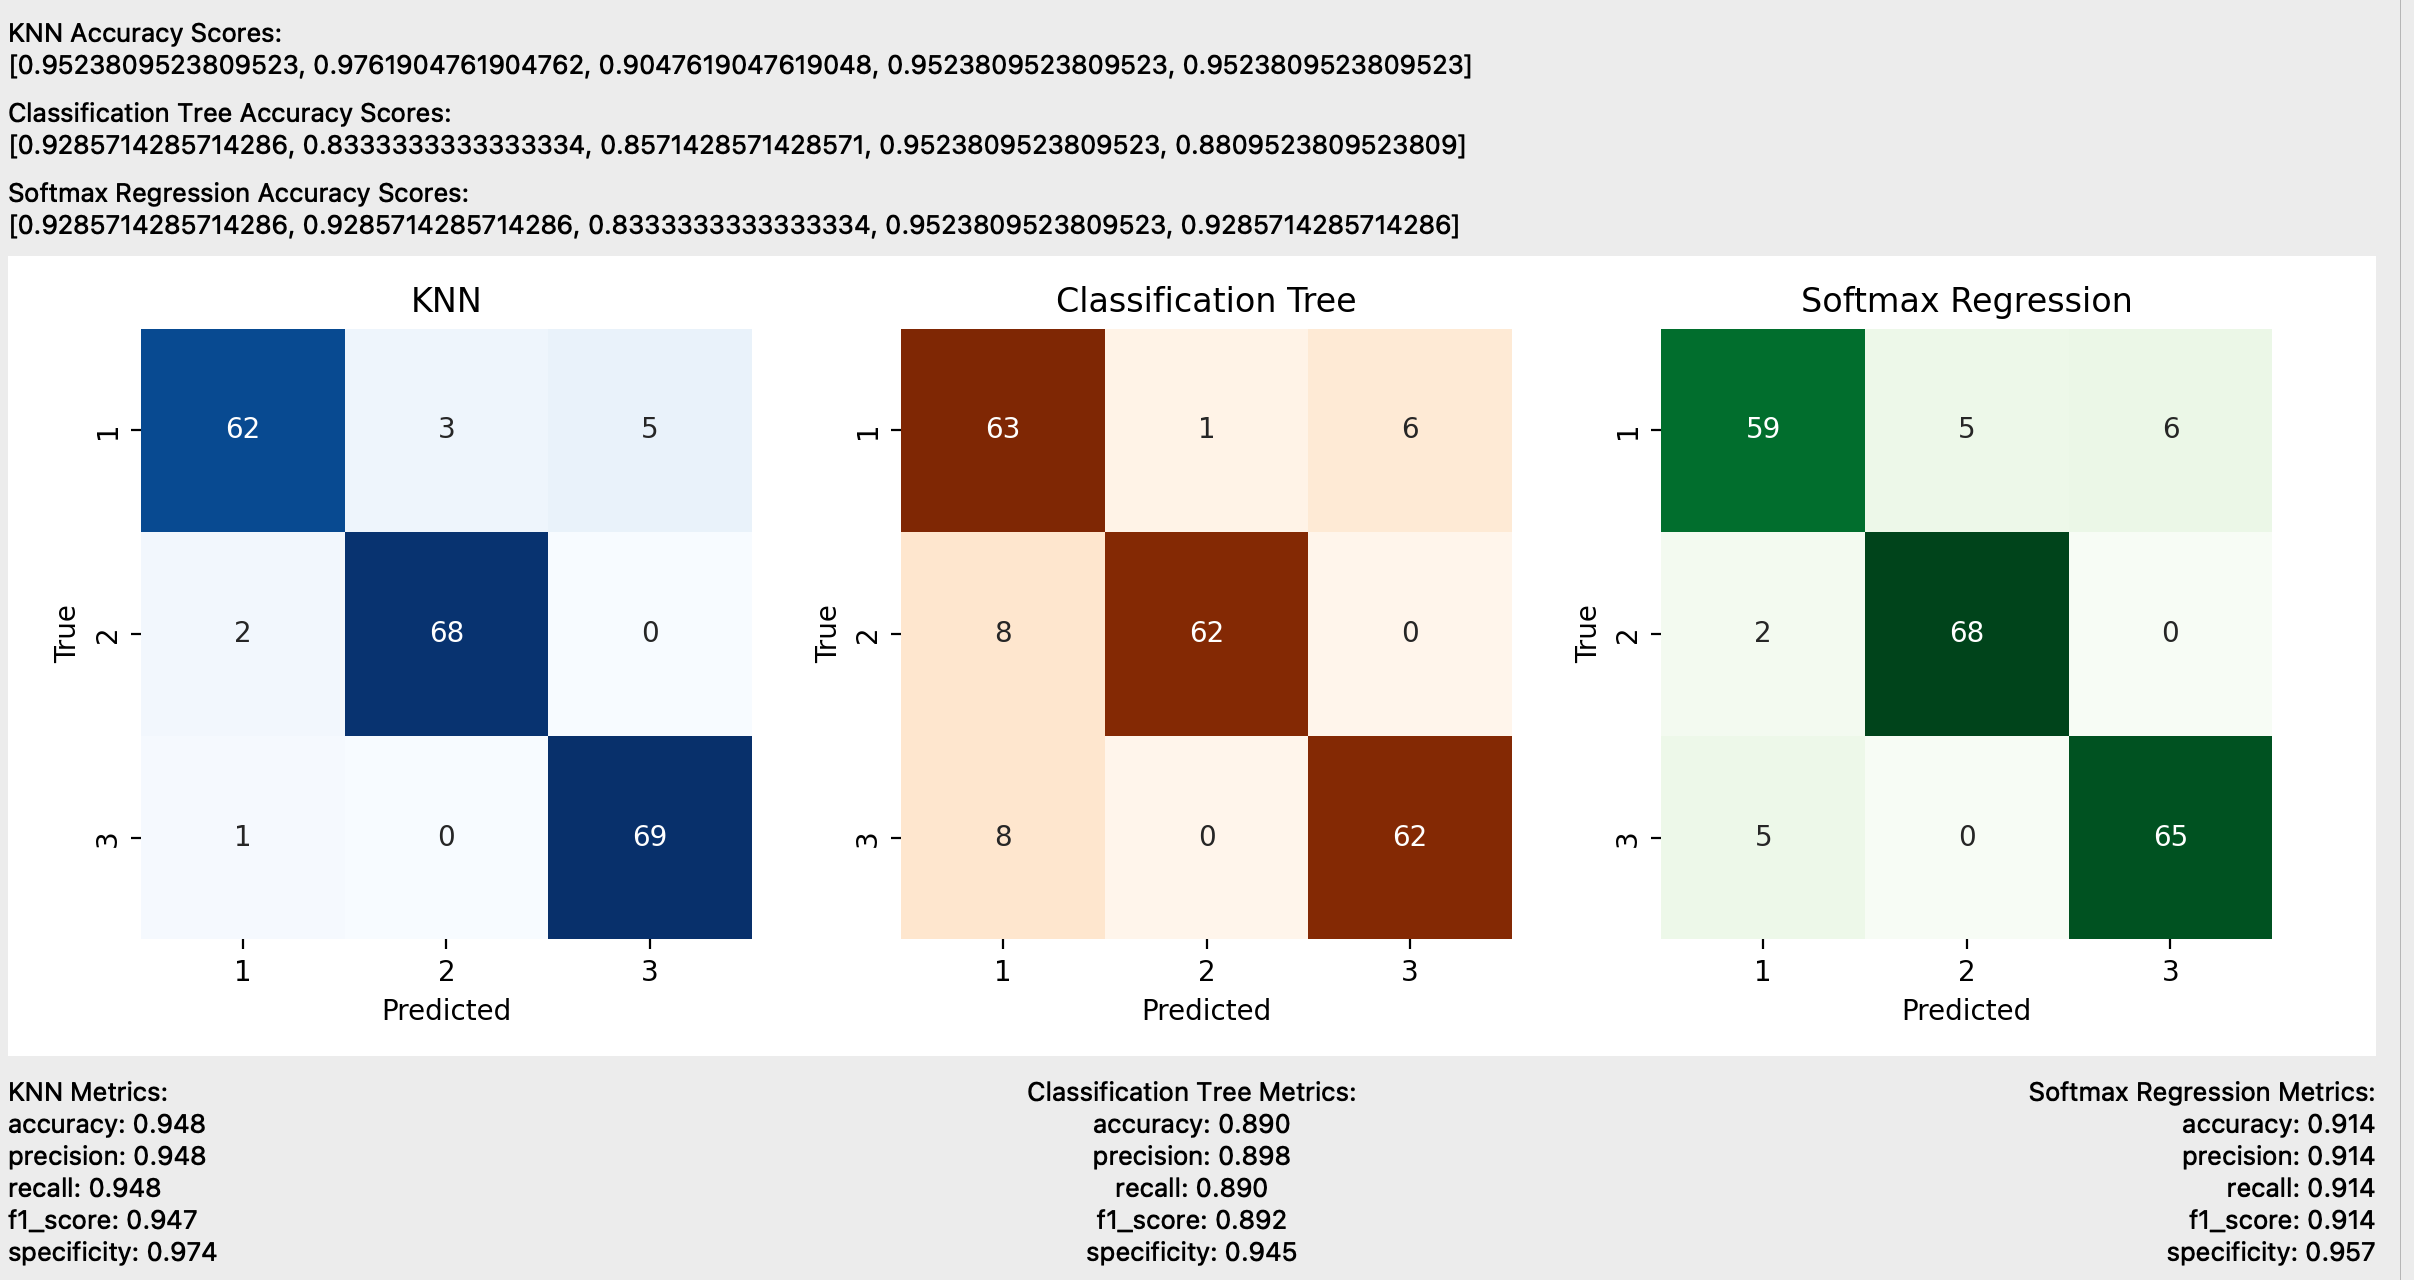
\includegraphics[width=1.0\textwidth]{seeds_results.png}
    \caption{Seeds Results}
    \label{seeds_results}
\end{figure}
\begin{table}[ht]
\centering
\caption{Performance metrics for each model on the Seeds dataset}
\label{tab:seeds_metrics}
\begin{tabular}{|l|c|c|c|}
\hline
\textbf{Metric} & \textbf{KNN} & \textbf{Classification Tree} & \textbf{Softmax Regression} \\
\hline
Accuracy & 0.948 & 0.890 & 0.914 \\
\hline
Precision & 0.948 & 0.898 & 0.914 \\
\hline
Recall & 0.948 & 0.890 & 0.914 \\
\hline
F1-score & 0.947 & 0.892 & 0.914 \\
\hline
Specificity & 0.974 & 0.945 & 0.957 \\
\hline
\end{tabular}
\end{table}

\subsubsection{Observations}

Based on the performance metrics, the KNN model achieves the highest accuracy of 0.948, precision of 0.948, recall of 0.948, F1-score of 0.947, and specificity of 0.974 on the Seeds dataset. This indicates that the KNN model is highly effective in classifying the wheat kernels into their respective varieties based on the geometrical properties. \par

The Softmax Regression model also performs well, with an accuracy of 0.914, precision of 0.914, recall of 0.914, F1-score of 0.914, and specificity of 0.957. This suggests that the linear nature of Softmax Regression is able to capture the discriminative patterns in the dataset and make accurate predictions. \par

The Classification Tree model has slightly lower performance compared to KNN and Softmax Regression, with an accuracy of 0.890, precision of 0.898, recall of 0.890, F1-score of 0.892, and specificity of 0.945. This may indicate that the tree-based approach with the specified hyperparameters (max depth of 3 and min size of 5) may not be as effective as the other two models in capturing the complex relationships between the geometrical properties and the wheat varieties. \par

Looking at the accuracy scores within each fold (provided in the screenshot), we observe relatively consistent performance across the folds for all three models, suggesting good generalization ability and robustness to variations in the data.\par
Overall, the Seeds dataset demonstrates the effectiveness of machine learning models, particularly KNN and Softmax Regression, in accurately classifying wheat kernels based on their geometrical properties. These models can potentially assist in automating the classification process and improving efficiency in agricultural applications.\par

\subsection{Optical Handwritten Digits Dataset}

The Optical Handwritten Digits dataset~\cite{misc_optical_recognition_of_handwritten_digits_80} is a widely used dataset in machine learning for the task of handwritten digit recognition. It consists of a large collection of grayscale images of handwritten digits, ranging from 0 to 9. The goal is to accurately classify each image into its corresponding digit class.

The dataset used in this analysis contains over 10,000 samples, providing a substantial amount of data for training and evaluating the performance of different classification models. Each image in the dataset is represented by a set of pixel values, capturing the patterns and variations in handwritten digits.

\subsubsection{Model Tuning}

To optimize the performance of the models on the Optical Handwritten Digits dataset, we conducted a model tuning process. The best hyperparameters for each model are presented in Table \ref{tab:digits_tuning}.
\begin{figure}[ht]
    \centering
    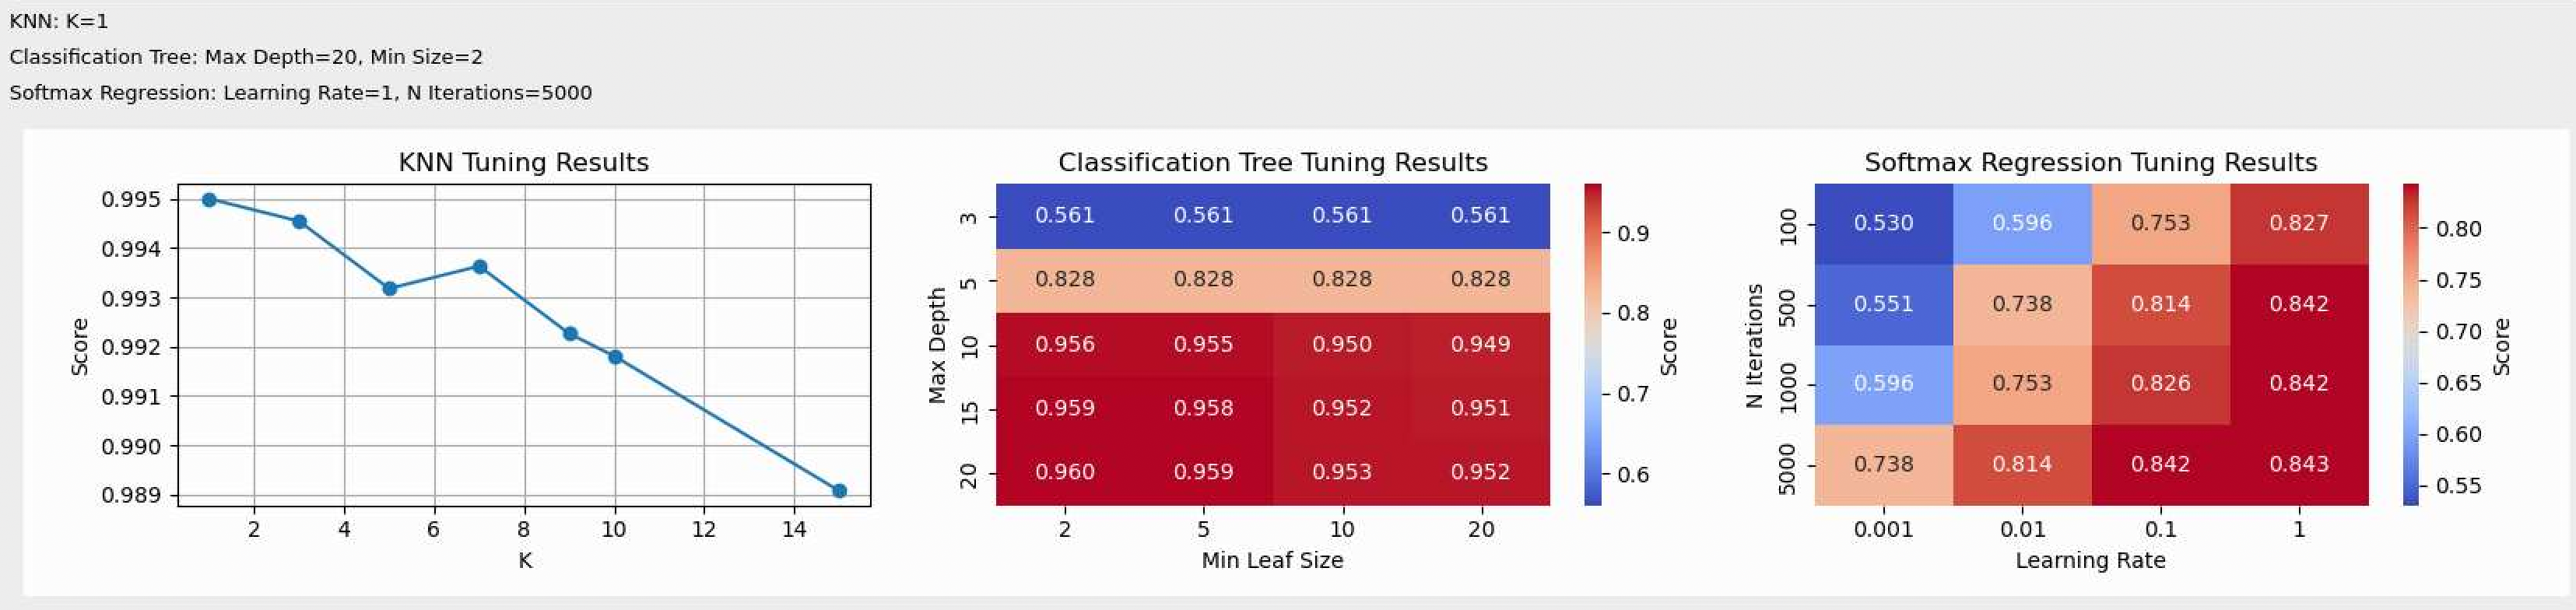
\includegraphics[width=1.0\textwidth]{pendigits_tuned.png}
    \caption{Handwritten Digits Tuned Models}
    \label{pendigits_tuned}
\end{figure}
\begin{table}[ht]
\centering
\caption{Best hyperparameters for each model on the Optical Handwritten Digits dataset}
\label{tab:digits_tuning}
\begin{tabular}{|l|l|}
\hline
\textbf{Model} & \textbf{Best Hyperparameters} \\
\hline
KNN & K = 1 \\
\hline
Classification Tree & Max Depth = 20, Min Size = 2 \\
\hline
Softmax Regression & Learning Rate = 1, Iterations = 5000 \\
\hline
\end{tabular}
\end{table}

\subsubsection{Model Evaluation}

We evaluated the tuned models using 10-fold cross-validation and obtained various performance metrics. The results are presented in Table \ref{tab:digits_metrics}.
\begin{figure}[ht]
    \centering
    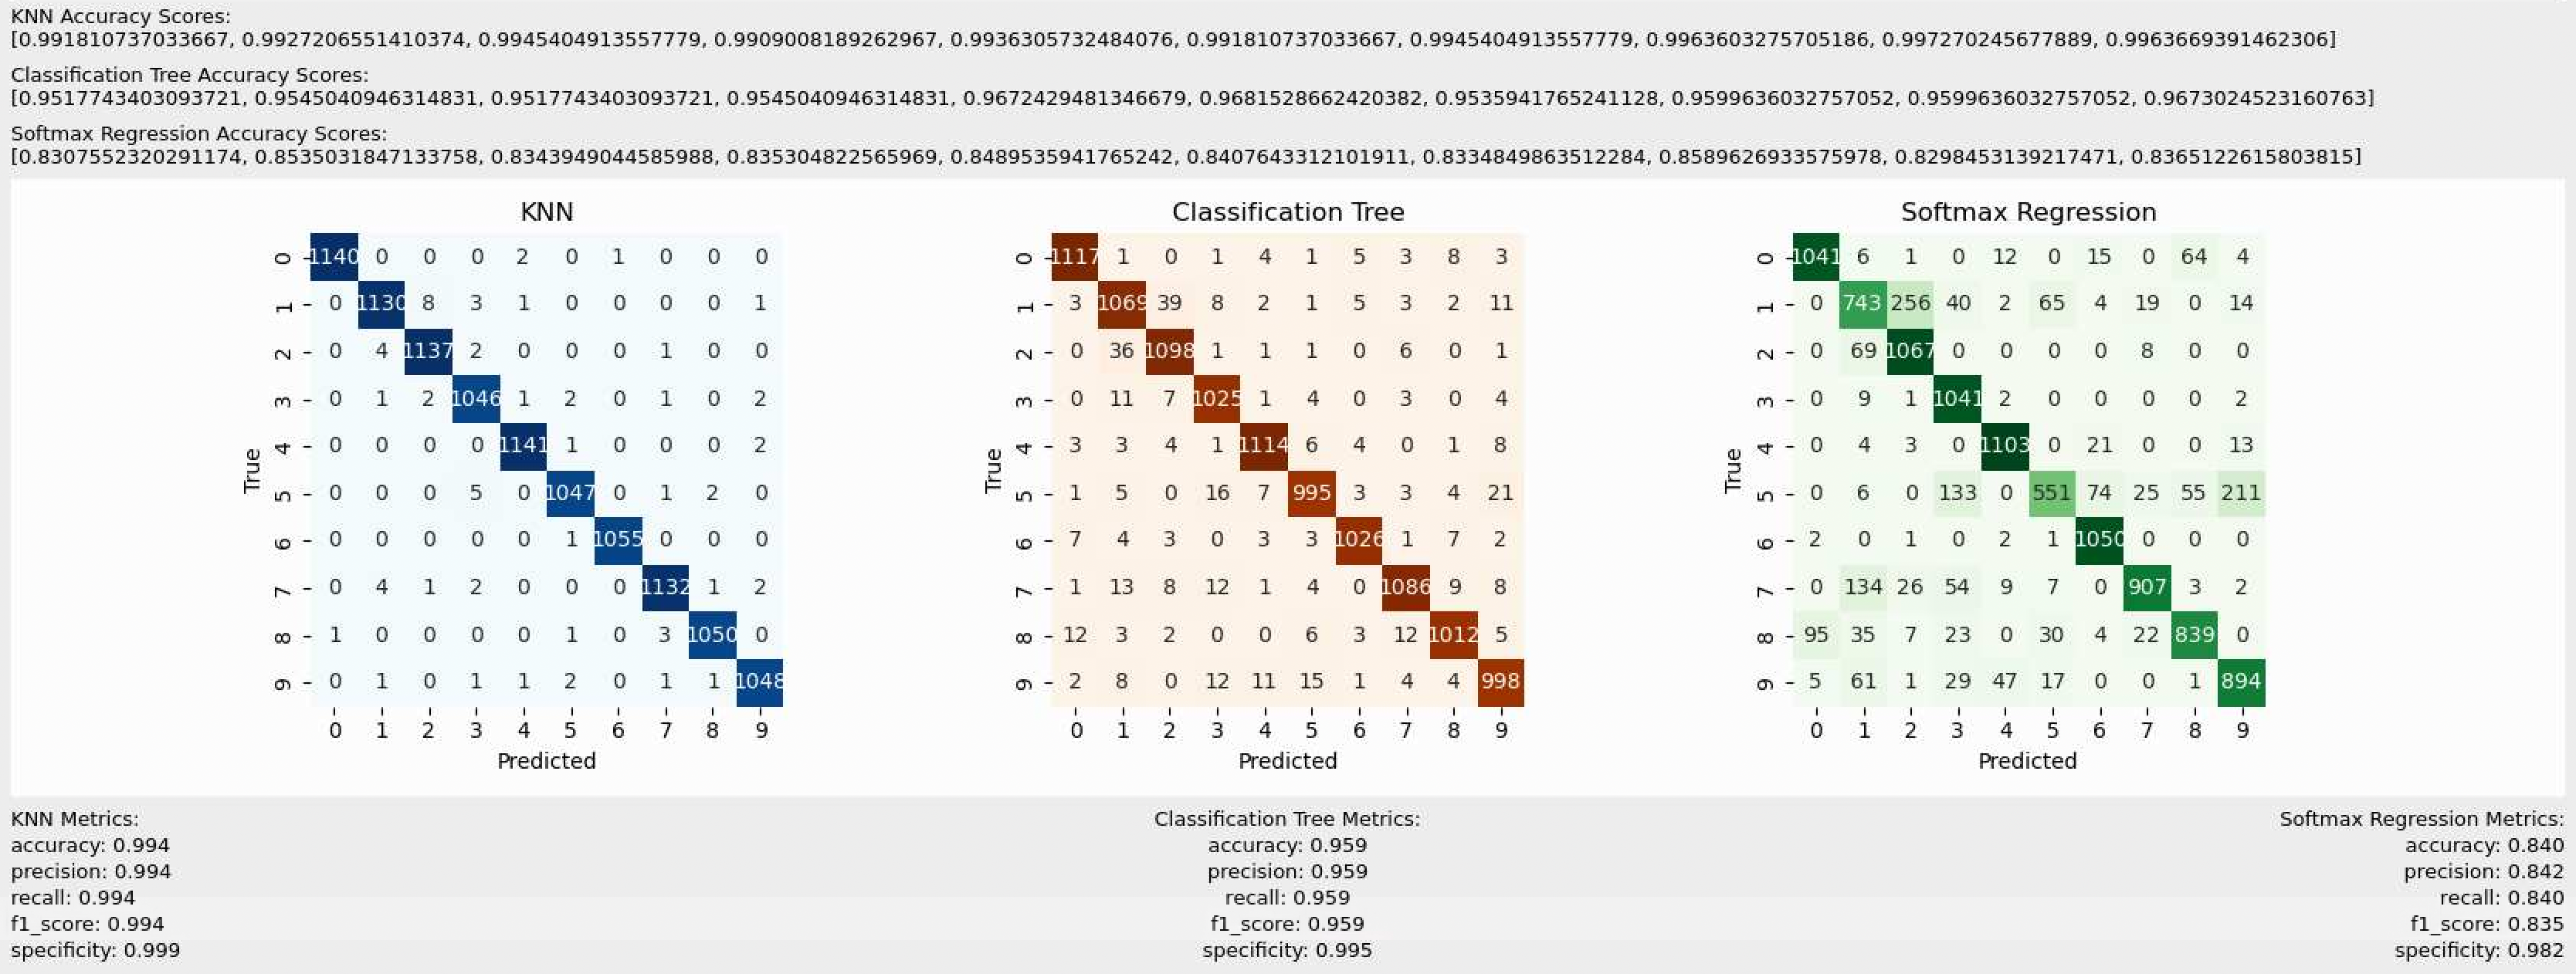
\includegraphics[width=1.0\textwidth]{pendigits_results.png}
    \caption{Handwritten Digits Dataset Results}
    \label{pendigits_results}
\end{figure}
\begin{table}[ht]
\centering
\caption{Performance metrics for each model on the Optical Handwritten Digits dataset}
\label{tab:digits_metrics}
\begin{tabular}{|l|c|c|c|}
\hline
\textbf{Metric} & \textbf{KNN} & \textbf{Classification Tree} & \textbf{Softmax Regression} \\
\hline
Accuracy & 0.994 & 0.959 & 0.840 \\
\hline
Precision & 0.994 & 0.959 & 0.842 \\
\hline
Recall & 0.994 & 0.959 & 0.840 \\
\hline
F1-score & 0.994 & 0.959 & 0.835 \\
\hline
Specificity & 0.999 & 0.995 & 0.982 \\
\hline
\end{tabular}
\end{table}

\subsubsection{Observations}

Based on the performance metrics, the KNN model achieves exceptional results on the Optical Handwritten Digits dataset, with an accuracy of 0.994, precision of 0.994, recall of 0.994, F1-score of 0.994, and specificity of 0.999. This indicates that the KNN model, with K=1, is highly effective in recognizing and classifying handwritten digits accurately.

The Classification Tree model also performs well, with an accuracy of 0.959, precision of 0.959, recall of 0.959, F1-score of 0.959, and specificity of 0.995. Although slightly lower than the KNN model, the Classification Tree still demonstrates strong performance in capturing the patterns and distinguishing between different digit classes.

On the other hand, the Softmax Regression model shows relatively lower performance compared to KNN and Classification Tree, with an accuracy of 0.840, precision of 0.842, recall of 0.840, F1-score of 0.835, and specificity of 0.982. This suggests that the linear nature of Softmax Regression may not be as effective in capturing the complex patterns and variations present in handwritten digits.

Looking at the accuracy scores within each fold of the 10-fold cross-validation (provided in the screenshot), we observe high consistency and stability across the folds for the KNN model, indicating its robustness and generalization ability. The Classification Tree model also shows relatively consistent performance across the folds, albeit with slightly more variability compared to KNN. The Softmax Regression model exhibits more fluctuations in accuracy scores across the folds, suggesting potential limitations in its ability to generalize well to unseen data.

\subsection{Summary and Conclusions}
\subsubsection{Model Performances}

\begin{itemize}
    \item \textbf{K-Nearest Neighbors (KNN)}: Demonstrated excellent performance in datasets where features displayed distinct clusters or were separable with minimal overlap, such as in the Breast Cancer Wisconsin and Optical Handwritten Digits datasets. The model's simplicity and effectiveness in capturing complex pattern distinctions with an appropriate choice of $K$ were notable advantages.
    
    \item \textbf{Classification Trees}: Provided robust results in datasets requiring decision-making that accommodates non-linear separations and categorical data. The model's flexibility was evident in its high accuracy in the Car Evaluation and Optical Handwritten Digits datasets, where a deeper tree structure captured intricate relationships effectively.
    
    \item \textbf{Softmax Regression}: While generally effective in scenarios with linear decision boundaries, such as the Iris dataset, it struggled in more complex datasets like the Optical Handwritten Digits. The linear nature of Softmax Regression limited its ability to model the high-dimensional, non-linear interactions present in more complex datasets. There's a chance that altering the regularisation parameters more could shed more light on this.
\end{itemize}

\subsubsection{Strategic Insights and Recommendations}

Based on the findings from various analyses, several strategic insights have been gathered to guide future projects:
\begin{itemize}
    \item \textbf{Model Selection}: It is crucial to align the choice of model with the dataset characteristics. Non-linear models are preferable for complex pattern recognition tasks (e.g., image data), whereas linear models may suffice for datasets with clear linear separations.
    
    \item \textbf{Hyperparameter Tuning}: Effective tuning of model parameters is essential to maximize performance. This involves not only selecting appropriate values for parameters like $K$ in KNN or depth in Classification Trees but also considering computational efficiency and potential overfitting.
    
    \item \textbf{Feature Engineering}: Enhancing models' performance, especially in linear models like Softmax Regression, can often be achieved through thoughtful feature engineering. This may include generating new features or transforming existing ones to expose new patterns to the learning algorithm.
    
    \item \textbf{Ensemble Techniques}: Employing ensemble methods can leverage the strengths of multiple models to improve predictive performance and robustness. This approach is particularly valuable in dealing with heterogeneous data or when a single model's assumptions are too restrictive.
\end{itemize}

\subsection{Conclusions}

Through systematic evaluation across diverse datasets, this study has highlighted critical aspects of model capabilities, offering actionable insights for deploying machine learning models effectively. Our analyses suggest that understanding the underlying data characteristics and aligning them with the appropriate machine learning models and techniques can significantly enhance predictive performance and decision-making processes in various applications.

\newpage
\section{Evaluation and Reflection}
When comparing the milestones of this project with my goals outlined in section \ref{successcriteria} from the interim review, I think I successfully implemented all the remaining functionality that my project was lacking to bring forward a far more well-rounded application. \par
Looking at the project more holistically, I do think I've delivered on my project title - I've quite rigorously compared the performances of three known machine learning algorithms on public, raw datasets with demonstrable results in the previous section. \par
I feel quite fortunate to be working on such a relevant project topic and I've learned so much during this process. In this section I'll list some issues I faced in this term and how I may try to amend them moving forwards.\par



\subsection{Issues and Improvements - Implementation}

\subsubsection{Fixed L2 Regularisation Lambda}
Regularisation is quite a key aspect of the Softmax Regression algorithm, which is why I ensured that it was implemented. Though it was added rather late, and though it's present in the model's training process, the value is not changed nor searched during grid-search. Due to this, all comparative performances of this model have lead to a recurring thought - how would it do if Lambda was a different value? With more time, I'd find a way to introduce lambda to the grid search. This issue is connected to the next one. \par

\subsubsection{User Cannot Change Parameter Grids}
Though I managed to allow the user to alter the evaluation process, I very much wanted to allow the user to alter how tuning worked too. I thought about this for a long time, but I struggled with how to visualise the possibility of three-dimensional grids without much time to alter how visualisations work in my project. I also simply wasn't sure how grid searches work with more than two parameters. This would likely be the next thing I implemented to the project given more time. \par

\subsubsection{Lack of Preset Datasets}
Purely for demonstration purposes or for checking that background operations are still operational, I did want this application to have preset built-in datasets to play with, rather than forcing the user to find their own  and leave them to hope that their data will fit with my app's constraints. I wanted to build an app that helped others learn about machine learning and I felt that this would have been a noteworthy component with benefits for all. \par

\subsubsection{Clunky UI}
UI was never a priority to me when entering this project, however it really is just ugly. More critically, it's not obvious how to navigate around it to someone new - and I'd very much like to change this. 

\subsubsection{Computationally Inefficient}
This app works much slower than I'd like it to, despite how large the datasets I'm working with are. It took possibly an hour for this app to evaluate the three models on the handwritten digits dataset, with 10,000 features.


\subsection{Adjusting My Approach}
\subsubsection{Hesitance to Experiment}
This has come to mind more often but I've realised that beyond just "time management" when it comes to my attitude to work, I've often hesitant to take action unless I'm fully certain I fully understand what direction that will lead me to, with full understanding of the material. This project has taught me that sometimes the best way to understand something, is to watch something go wrong. \par

\subsubsection{Committing Small and Often}
I noticed that the phases of lack of activity with this project were simply when I hadn't made a large contribution to it in some time, often due to the previous issue. Besides taking courage into my work, I've also learned that mountains can turn into manageable work if things are broken into pieces. \par
\subsubsection{Final Thoughts}
Overall, I do find myself leaving this project behind feeling more confident of myself as a student, an engineer and an individual. I feel a lot of gratitude for the opportunity and the support that's been given, I've learned a tremendous amount not only from staff but from peers. \par

The final lesson I'll take from this, is I've understood that it is very easy to do things like this on our own with our own initiative. This project has given me the tools and experience to build useful and robust products, and I'm excited to embark on the next one.
\newpage
\bibliographystyle{IEEEtranN}
\bibliography{bibliography}


\appendix

\section{Appendix}
%TC:ignore
\subsection{User Manual}
A user manual has been attached to the page below.
\begin{markdown}
## Project Installation and Execution Guide

Welcome to the project! Here's a quick guide to get you started.

### Prerequisites
Before you begin, ensure you have Python installed on your system. You can download Python from [python.org](https://www.python.org/downloads/).

### Installation
First, you need to unzip the downloaded repository. Once unzipped, navigate to the project's parent directory where the `src` folder resides.
### Running the Project
To run the project, execute the following command from the parent directory of the `src` folder:
    

```
python src/main.py
```

   
This will start the main application.

### Troubleshooting Dependencies
If you encounter any issues related to missing or incorrect dependencies, you may need to install or update some dependencies. This can be done by entering the src folder and running the following command:

    
```
pip install .
```

   
This should update and install any required dependencies.



\end{markdown}
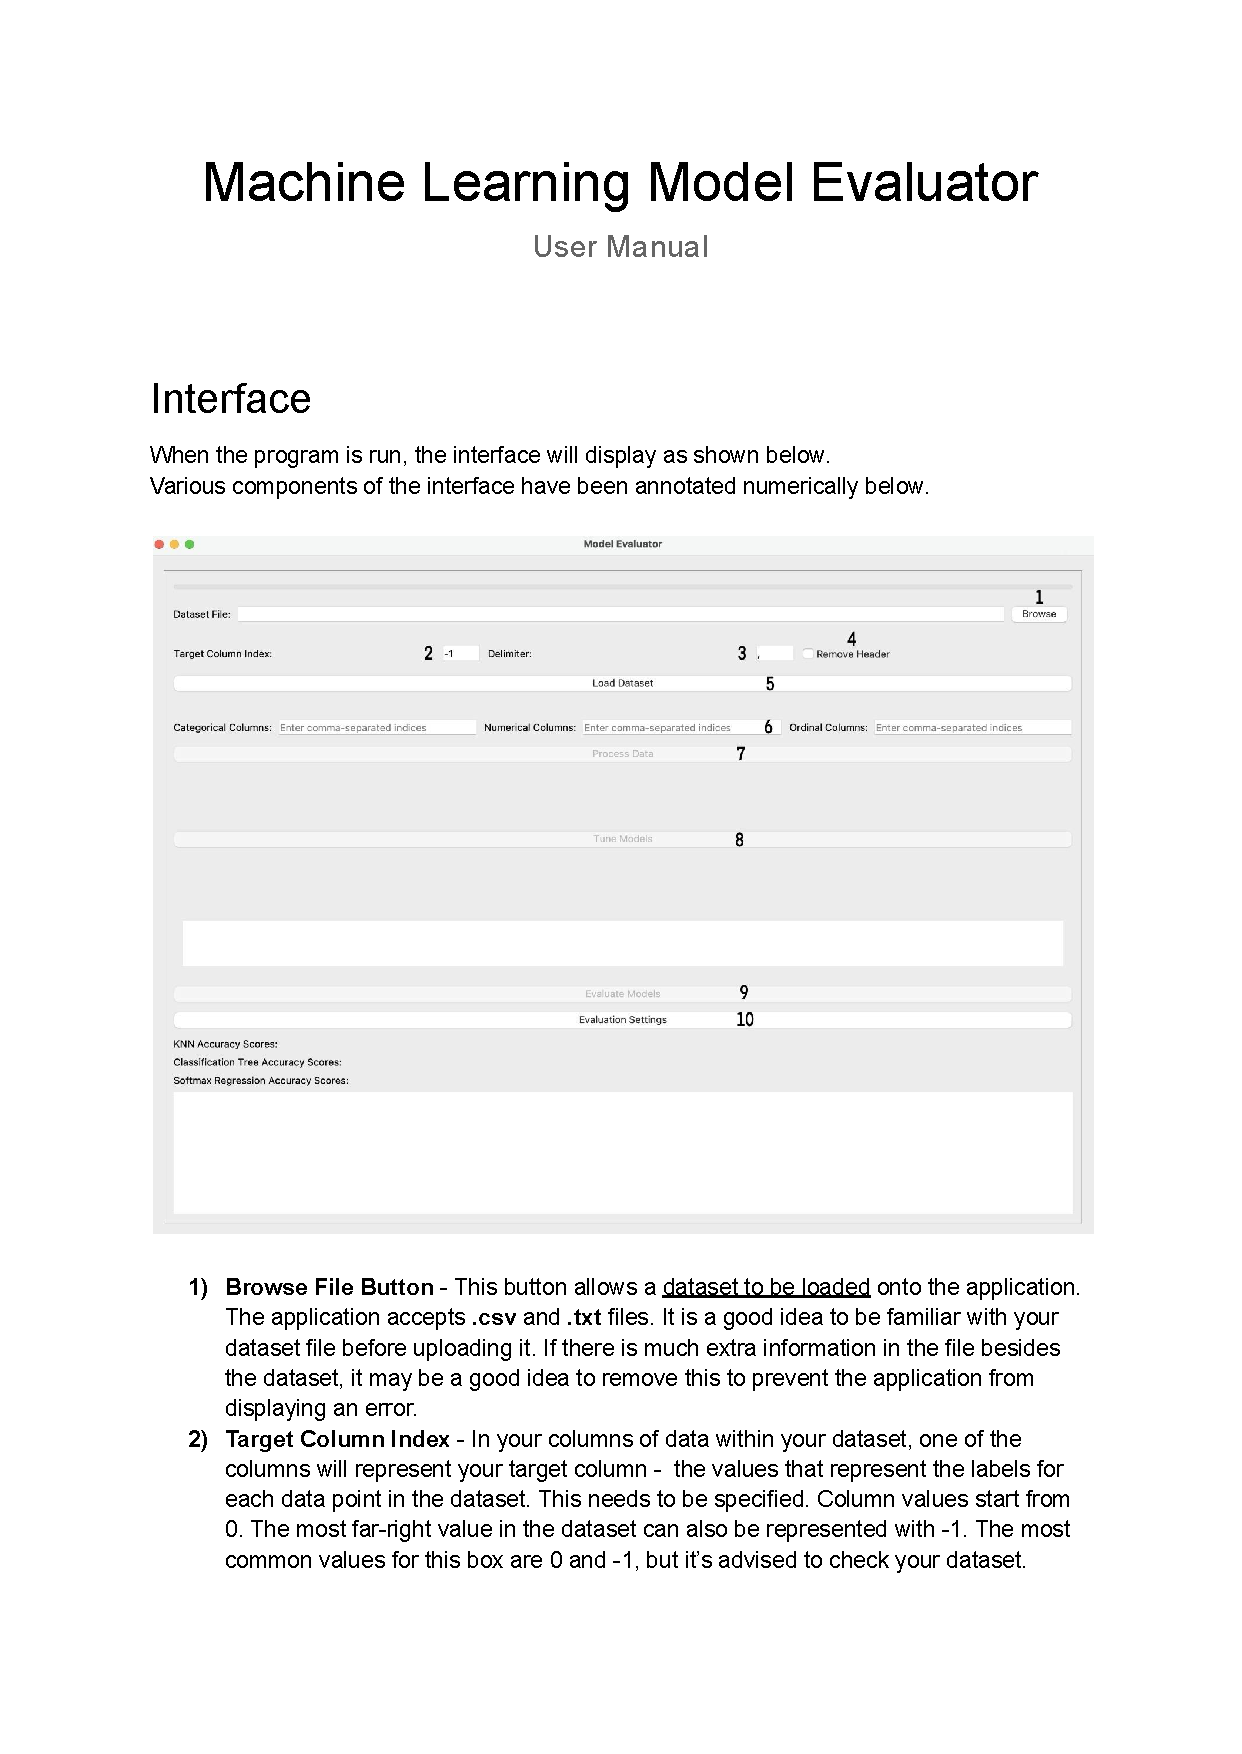
\includepdf[pages=-]{UserManualFYP.pdf}
\subsection{Diary}
The diary appended below is in rather informal shorthand but illustrates my honest thought process while approaching and delivering the project. The diary can be found in the diary folder of the project repository, titled "FYP-diary.MD"
\begin{markdown}


_(Updated 11/04/24)_

### 18th September 

Allocated supervisor and informed by supervisor of my project title (allocated on 15th September). Supervisor will be Prof. Zhiyuan Luo.
Project will be Comparison of Machine Learning Algorithms.

- Made notes and research on "Breaking the ties" with K-NN algorithms
- Made notes and basic research on Uniformity with Decision Trees, noted measures of uniformity (Gini, Entropy, Info Gain) - will need to read more about these soon.
^^ Both points are highly relevant for the early deliverables.

Watching CS229 ML lecture [video](https://youtu.be/jGwO_UgTS7I?si=TcRudZ_jwvuylEkv) given by Andrew Ng at Stanford, 2018: 
Very easy to absorb lecture on overview of different types of ML. My project so far seems to be directed towards Supervised Learning-Classification



### 19th September

Attended Project Talk given by Dr Argyrios, covered 2 presentations. Useful talk, Argyrios clarified to me personally that LaTeX Project Plan can be in any format, isn't an institution-locked layout.
Heavy emphasis on focusing on project plan.

As of writing, the outline of plan is somewhat structured, but much work needs to be done.

Will meet Prof. Zhiyuan on 25th, guidance given on how to access his office

### 20th September

Started trying to plan my meeting with Prof. Zhiyuan. Many questions to ask, just trying to find the right questions. Noted that there are various paths I can take this project, now considering if I should exclusively focus on Classification.
Noted that it's difficult to research on Classification without needing to read into Regression techniques. There's also lots of notation to digest.

- Understood the functionality of parameters (theta) alongside features/inputs (x). Learning a lot on notation in ML. The algorithms given in the brief seem to be more-or-less non-parametric, however - though I could be mistaken.
- Research on kernel functions and how they transform data into a different representation such that data is easier to evaluate and more separable. I understand this very superficially. Need to read more on examples: Linear, Polynomial, Gaussian (RBF) and Sigmoid Kernels.
- Some basic research on Multi-Class Support Vector Machines("one-vs-all", "one-vs-rest"). Complicated for now, will be useful for final deliverables. Also tribute to Vapnik. 
- Research on RSS (Residual Sum of Squares) Criterion - not sure if relevant to KNN/Trees/Classification algorithms, seems moreso relevant to linear regression
Started watching CS229 [Lecture 2](https://youtu.be/4b4MUYve_U8?si=GvrB1HdXNJ66JWNE), very useful information on notation by Andrew Ng, mostly focused on Regression however. 

- Some concerns that I'm mostly focused on theory and not so much on implementation. Started digging around sci-kit learn [documentation](https://scikit-learn.org/stable/modules/tree.html) today: - will continue to get familiar in upcoming days.

Upon arrival at campus, I've borrowed 5 books from library physically:
1. The Elements of Statistical Learning, 2nd Edition. (TEoSL)
2. Pattern Recognition and Machine Learning by Bishop. 
3. Foundations of Machine Learning by Mohri
4. Introduction to Machine Learning with Python by Muller & Guido. (MLwP)
5. Hands-on Machine Learning with Scikit-Learn and TensorFlow

Primarily I've been using (1) TEoSL as reference and using the others, or the internet to decipher concepts or notation when it's difficult to at first glance.
I've not been using (4) yet but I think it will be vital as I start making proof of concept programs. 

Today found out from Prof. Vovk via Moodle that a new textbook has been released online: An Introduction to Statistical Learning with Applications in Python, 2023. It seems to be a simpler version of TEoSL, so it might be the perfect resource for me. I'm in luck!
Exchanged emails with the library services today but book isn't available physically, they've provided me an online copy. 

GitLab repo is online! Aiming to put this diary on there.

-Research on using OverLeaf (LaTex editor) in sync with GitLab such that I can track version history of my reports. Also research on Git, branches and recapping version control studies. Emailed Prof. Argyrios for confirmation of repo, as well as gitlab classes and slides from earlier talk. 

### 21st September

Made various changes and commits to repo last night and this morning, it now contains folders for this diary and the project plan I'm working on in LaTeX. I've been pushing to master(or main) lately and it doesn't feel right to me - so now that I've made my repo somewhat easy to navigate, I'm making a branch to continue research on: plan

I'll use the planning branch up until my Project Plan is complete, I can then use my repo to explore my research and put proof of concept programs for the algorithms together while I'm still trying to define my project. This branch will represent my initial development phase. I've spent a lot of time last night and this morning keeping up to date with git conventions such that everything is done orderly. Creating this branch felt like the natural thing to do in this formative phase of my project. My intention is to merge the plan branch with main around when the Project Plan is complete and submitted, marking the beginning of development (and likely, a new dev branch).

I purchased a pocketbook for meetings and ideas with my supervisor

I will spend today looking at sci-kit learn and trying to play with library functions that have implements knn and decision trees already. I have barely looked into datasets yet and I must do so, this will likely define the direction of my project. Still need to look into whether Classification is what I want to exclusively work on. I will also work on my Project Plan, this should be a priority.

### 22nd September

Yesterday I continued reading about kernel functions and SVMs and honestly - found myself overwhelmed with theory and how much I still need to understand, let alone bring to the meeting on 25th. I think I need to focus more now on implementation. I'll work on the simplest ML algorithms and focus on implementing them and assessing them, further theory can wait I think.
I aim to now focus on working through the exercises in MLwP and get familiar with working with datasets.
Yesterday I also found Kaggle as a useful resource for datasets. Kaggle is the largest open-source ML community and it's highly likely I'll use their resources in this project, along with UCI and Delve, as long as the data isn't too difficult to process.

Also thinking of turning these diary files into markdown format for easier use.

Setting up python and Jupyter on macOS surprisingly time-consuming.

### 23rd September

Been playing with GUI elements today, tkinter and pyqt5 - I've not really decided how the end-product of this project is going to look and function, so I started investigating this today.
Wasted a ton of time configuring python environments.

Spent good amount of time today planning for meeting, have a decent outline of things to cover. In the process, have structured my approach to tackling the project a little better.

### 24th September

Wrote meeting outline for supervisor before tomorrow's meeting, during the process did a lot of research on model evaluation concepts and metrics

Sent email with a decent amount of detail, very much looking forward to the meeting. I feel this has been a productive week but I need to make many decisions still on how I'm going to tackle this project.

Will likely change these to .MD files tomorrow and perhaps make a research folder. Hoping to start implementing Jupyter Notebook projects next week.

My priority next week however, will be my project plan. 

### 25th September

Met supervisor! Meeting was thoroughly helpful. Main takeaway from meeting was to 'keep it simple'. I will focus on Nearest Neighbours for now and try implementing the simplest variation of this algorithm in handwritten form. Doing this will allow me to fully understand the algorithm at its core.
I'll likely just focus on simple implementations of Nearest Neighbours, Decision Trees and perhaps Logistic Regression - I need to read more into this.

My priority is the Plan right now, I think I know which reports to focus on for this term at least. I should start with mathematical implementations of the algorithms to further my understanding - and this might help while I'm creating the Plan. I should then get started on building the algorithm and can structure my approach in SE terms via the Plan too. It's clearer to me now that the Plan is a tool to help me, rather than just a deliverable for assessment.

### 27th September
Attended FYP Talk on LaTex and Referencing today. Since classes have started, it's gotten a lot busier and less time to focus entirely on research and project progress.

Additions have been made to Project Plan abstract. I hope to have an outline of some kind prepared by Friday and ideally a draft before the end of the week which can be reviewed by my supervisor.

I've forgotten to mention that I've been using a 6th physical book by Tom Mitchell called Machine Learning for much of my research. I find it easier to absorb theory on there, and it covers decision tree theory in much more detail than TEoSL. I think it's probably much more suited for Classification problems.

### 28th September
Following the previous FYP talk, I've started using Google Scholar to find papers to use as references - and already found some great authoritative texts on the NN algorithm.  
I aim to make real headway on the Plan today and I really hope to complete some kind of draft by tomorrow, such that I can get early feedback from my supervisor. Today I really need to make some executive decisions on the direction and goals of my project.  
I've decided it may be wise to include some kind of _success criteria_ in my Abstract, such that I can make critical goals to deliver for the interim review. This project is so open to expansions that it's important to define what should be expected by the end of this. Creating a set of possible expansions may make it more flexible. Once I start assigning a time-frame to this project, it'll become clearer.

### 15th October
It's been a while since the last diary entry.
Unfortunately, I may have underestimated how challenging it would be to balance the project with the other modules I'll be studying.  
The week following my last entry was entirely focused on implementing my Project Plan and submitting something that motivated and outlined my approach to the project sufficiently.  
The week after this should have been focused on developing my proof of concept programs, designing my UMLs and beginning my Nearest Neighbours report. Unfortunately, last week was not fruitful and I'll have to spend this week catching up with my outline immediately.

### 16th October
I've made small progress with the NN algorithm proof of concept and it works as expected. The labs in my machine learning module have been very useful with learning python syntactic sugar and dealing with datasets in Jupyter Notebooks. I'd like to somehow implement some kind of unit testing this week that I can carry forwards for the rest of term.  
The repo needs to progress to a new branch for development and I hope to do this immediately after this entry. I'll be transferring from the 'plan' branch to a 'dev-poc' branch, updating the main branch in the process. It's likely that this will be the first of many dev branches in the overall process.  
I'll need to update my README too with all the new structure I have put in place.   
I'll likely setup some structuring of my interim and supplementary reports(NN) this week.  
I'll move forwards with haste, and hopefully hear feedback on my outline soon, just to find if it's too ambitious, though I feel I'm already seeing that it is. 

### 2nd November
With the start of November, I do feel that I'm falling behind, not only with the work outlined in my plan - but also unfortunately, the diary entries. I do hope to make these more frequent and get back on track with my weekly diary entries.  
  
I've made progress on Nearest Neighbours and K-Nearest Neighbours proof of concept programs in Jupyter Notebooks. I realised quite quickly that it was imperative to create train-test-split functionality immediately just to test these algorithms functionally, and I've managed to do so.  
I think that my implementation of train-test split will help in implementing k-folds cross-validation.  
I've essentially realised that I need to implement model evaluation functions in conjunction with my models otherwise it's difficult to know if I'm going the right direction with my model implementation.  
  
If I focus on completing an implementation Nearest Neighbours and beginning an implementation with the Tree algorithm - which I believe will carry its own challenges - before the end of this week, as well as implementing cross-validation in some way. I may be able to catch up with my plan's outline.  
  
I'm moreso worried about making progress on my reports, as I'm very behind on this and I believe this will be more time-consuming than the algorithm's implementation. I'll be making immediate work on the NN algorithm report, and have already built the skeleton of the report in LaTeX.  
My only consolation with this is that I don't feel lost with the theory of this much at all and I think research should be straightforward thanks to the reading I did out of interest during the summer.  
  
I had my second supervisor meeting a week ago, and the main theme of this meeting was that I essentially need to simply put my head down and deliver. My understanding is there, I simply need to push work forwards without fear of making errors.  
  
Areas that I might need to look into next week include handling missing data in datasets and how to implement PyUnit tests for my validation functions. I've played with a heart disease dataset from the UCI repository and noticed that handling missing values might be a challenge that I need to focus on within my data preprocessing phase.  
  
CS3920 lectures and labs have been handy for me looking ahead, and I think investigating normalisation techniques and how they affect model accuracy may be something to do next term.  
  
All in all, I'm running behind, I'm aware of it, and I need to move quickly to catch up in time for the interim review.
  
### 15th November
I attended the FYP talk today by Prof. Dave Cohen about Presentations and how to bring forward our project during Presentation Week. I'm actually looking forward to talk about the research I've made. However I believe I'll need to make some compromises in order to deliver my targets on time, and I think this will have to take the form of the report deadlines set by myself.   
I've simply not been keeping up with working on reports in adjacent form with my development, along with the intense assignments I'm working on currently this month. I think I'll have to work solely on the interim report and put together my findings on the two algorithms concurrently within my interim report - rather than simply bringing in two completed algorithm reports to introduce within the interim report. Once the interim report submission is complete, I can review if I want to add more detail or background to the algorithm reports during the second term.   
It's likely that I'll need to perform some kind of review before the end of the the year to create a more thorough plan for Term 2.   
  
I've made some progress with the Decision Tree with Gini Impurity but still trying to work out how to introduce stopping criteria. I'm tentative to commit something that breaks.  
From the library, I've picked up the book by Leo Breiman - Classification and Regression Trees. It's verbose but goes into pretty deep detail about tree splitting, stopping and pruning strategies. I'm curious about introducing entropy/information gain but the benefits don't seem obvious to me unless I bring about categorical data into the mix - which I've just not done yet.  

I've discovered a really neat dataset on Kaggle called the Titanic dataset, it seems like a fun thing to bring in and a little more interesting than classifying flowers. I'd like to try and bring this into play before the end of term, but it depends on the difficulty of data preprocessing. I think it'd be nice to talk about for my presentation.  

Looking back at my early research, it's quite funny to see how much of the theory I was reading through is rather irrelevant to the implementation I'm putting together - (RBF Kernels, Multi-class SVMs) - and it makes sense now why my supervisor told me to keep things simple back during our first meeting.
  
### 24th November
Judgement day is almost upon us as my Interim Review deadline is approaching. I believe I have two functional algorithms deemed worthy for evaluation, though both could be extended in various ways.  
I now need to piece together my report and ensure I have sufficient notebooks that evaluate the algorithms' performance. I've not quite completed the cross-validation functionality, but I think I can have this complete in a few days.  
My third supervisor meeting has been scheduled for the 30th.  
I need to ensure I have a testing strategy in place that checks the robustness of the algorithms while I made alterations to them.  
  
I do feel that I could bring in a third algorithm into play during second term, to make things more interesting. I think after learning about SVMs in CS3920, I have an idea on how this could be a third classification algorithm I could use for comparison to KNN and Trees.

### 27th November
Since my last entry I've managed to implement K-Folds Cross-Validation, and made a few tweaks to my models such as adding a get_depth() function to my decision tree. I think my the end of today I can have Leave-One-Out Cross-Validation implemented (as it's essentially when K-Folds = N) with its own get_score functions.   
Implementing K-F CV feels significant as it seems to be the first time that all of these modules are working together, and seeing it work in the notebook has been satisfying, confirming that the data structures are all working as I'd hoped.    
One thing I'm a little disappointed about is how my algorithms don't yet work on datasets with missing data, or with categorical data - which significantly limits which datasets my models can work on. I have to make a decision on whether I can somehow implement this soon, or just focus on delivering my report and interim review.
   
I've managed to implement a more explicit way of handling ties within my KNN algorithm today.
  
I feel that I could find a way to automate some kind of "hyperparameter tuning" for my algorithms - I'm just currently unsure if this would lead to data snooping. From what I'm reading - it's important to use one hold-out set for hyperparameter tuning, and then a different test set for general performance. I'll need to clarify this with my supervisor. 

As for categorical data, I've been reading on how ordinal data and nominal data are generally handled - using one-hot encoding and label encoding. It seems to me that I may need to build some kind of encoder for my data in the future to handle future datasets. I've not considered normalisation - and it'll be necessary for me to implement this, particularly scaling, as if I want to start training on the breast cancer dataset and titanic data - which has missing data, but also a wide range of scales of data - I'll need to bring this forward soon.

On another note, today the deadline for the interim review has been postponed by a week. This is generally good news, but does make me a little confused about whether I should keeping implementing new changes - or wrap things up for review and focus on my report and presentation.

### 28th November
Having read more about normalisation, handling categorical data and missing data - I think it would be wise to delay this until after the review. I could try and quickly hash something together that works, but I do feel that I need to thoroughly research and plan this implementation out in such a way that they're integrated with model models smoothly.  
  
For KNN, there's a chance that I may need to implement a new distance measure such as Hamming Distance or Jaccard Distance to handle categorical data sufficiently, without making misleading effects to the distance between samples. 

### 29th November
I've managed to add various test suites to thoroughly check edge cases for the functionality implemented thus far. Doing this helped me notice gaps in my exception handling when passing values around - such as in K-folds and train-test-split when specifying the size of the fold or split. 

### 30th November
Today I finally had my third meeting with my supervisor. It went smoothly and my supervisor seems satisfied with my progress thus far. I managed to clarify doubts I had about the following:  
  
- Handling missing and categorical data:
  - For missing feature data, it's usually find to remove the entire sample for that instance. As long as there's enough data samples to make training sufficient.  
  - I asked about implementing an encoder to handle nominal and ordinal data, this seemed like a suitable idea.  
  - I asked about how this may affect the distance function in KNN, and if nominal data could be handled correctly, if I should using Hamming, Jaccard or Cosine function as an alternative. He suggested I keep trying with Euclidean as this should work okay with the situations I'm dealing with. He reminded me to just try it before I doubt the implementation.

- He cleared up misunderstandings I had about other performance metrics besides accuracy - such as the difference between Precision and Recall, and using the F1 score. I think I could quickly calculate these with the implementation I have so far. He also reminded me that I can find the variance of my model by analysing the range of accuracy values I find during K-Folds Cross-Validation.  
- Hyperparameter Tuning - I asked about the procedure of finding the ideal hyperparameters of KNN and Trees, i.e. the number of neighbours K for KNN and the maximum depth of the tree constructed. He reminded me to avoid data snooping, which I seemed to be doing in Notebook 6. I need to keep the test set separated and utilise a validation set for this.  
- He emphasised that it's very important that there's some form of data normalisation for KNN, as it's rather distance-sensitive. This may have explained unusually low values I was getting for the optimum k-value on large datasets such as ionosphere (though perhaps this is the curse of dimensionality in effect).  
  
Following the meeting, I immediately implemented a MinMaxScaler so that I have some form of data normalisation I can use to handle misaligned data ranges, particularly for KNN. I will need to correct my hyperparameter tuning procedure too.  
Overall in project development, I have built a pretty strong foundation for me to use for Term 2. I just need to show the results found on the three datasets I've chosen - iris, ionosphere and banknote authentication.  
Right now, my priority is putting the presentation and report together - this needs more urgent work. 

### 6th December
Obligatory diary entry - I've been working away at completing my deliverables for the interim review - the interim report and the presentation. The presentation has been submitted and will take place on the 8th.  
I'm finding it difficult to not add further functionality to the project last minute. I think there's still a lot I can do to automate various processes, such as the hyperparameter tuning process, and finding metrics such as accuracy. I think I can work on the preprocessing.py module this month after the review, and also work on integrating the process of calculating accuracy, recall and precision within a new metrics.py module.  
My report is coming together, it leans quite heavily into the theory. Overall, I do feel quite proud of what I've managed to do this term, and I think I can carry this momentum forwards, once submission is completed.
  
### 10th December
Term 1 is over! I gave my interim presentation on the 8th and it went very well, I received around four questions - two from the audience and two from the Chair. One member of the audience suggested I implement integer division into the way I calculate my folds for K-Folds Cross-Validation. I've realised now that I have already implemented this, but the need to handle the remainder is still necessary. I received further questions about how my MinMaxScaler was implemented, and why I chose the algorithms that I focused on.  
  
Lately, I've been thinking about what I may need to research on for the rest of this month to make next term a little easier for me.

### 17th December
I think the most immediate addition I'd need to make to my project should be the addition of some form of Encoder to handle missing data and categorical data. Handling this would quite immediately increase my algorithm's functionality and I'd quite rapidly be able to double the number of datasets I work with, and evaluate my algorithms a lot more rigorously.  
  
The Leave-One-Out Cross-Validation exposed just how inefficient my tree algorithm is during training - and I think I'd need to find ways to make the algorithm less greedy during the split search. I could also do some research on the ID3.5 algorithm to see how it differs to the CART algorithm that I've implemented.  
Another significant issue I need to bring my attention to, is how the tree model doesn't reveal much information about its structure, such as the number of training points that were classified at each leaf node. Finding this will make debugging and optimisation significantly easier, and could potentially help me devise a method of finding a confidence level for each prediction.  
  
A key objective in the next term will be to work on an interface for these models to work, and essentially, act as the front-end of my final project. I've not made a start on this, so it'll be wise for me to at least research which libraries I'll use to put this together.  
  
Pipelines were mentioned towards the end of the CS3920 ML course - I feel like this could be a solid addition to my implementation. The interim submission shows each process executed manually - and this simply won't be feasible in a graphical interface layout in Pipelines. I think pipelines could help me to wrap up all the preprocessing in a neat way, as well as potentially show off some intricate software design practices.  

I've yet to use Precision and Recall as metrics in my project, and it seems silly to only use accuracy as a sole metric so far. However I've noted that these metrics are generally only used in binary classification - so it'll be necessary to adapt this for multi-class classification. 
  
### 16th January
I'm gearing up for the upcoming term and I've comprised a list of necessary objectives:
  1) Preprocessing - Handling missing and categorical data to accommodate more datasets
  2) Tree Refinement - Implement optimisations to how the tree searches for splits during the training process. Alter the tree model structure so that the leaf nodes are more informative.
  3) Metrics - Introduce more model evaluation metrics that allow more thorough comparison and insight into the algorithms' performance. 
  4) Pipelines - Implement pipelines that can encapsulate much of the data manipulation into few executions. This will make it easier to implement an interface for the end-user. 
  5) GUI - Make a head start in implementing a simple but effective graphical interface for end-user to use the algorithms being discussed. Ideally allow for inputted datasets to be analysed and trained upon. 
  6) Implement a third algorithm given there's enough time to do so. Strongly considering logistic regression.  
    
I'm relieved to have received positive feedback on my project's progress so far, as well as the presentation - It's assuring to know that my implementation so far is going the right direction.  
  
I'm likely to have a lot more clarity over next steps after my next supervisor meeting. 
  
### 25th January
Just had my 4th meeting with Zhiyuan - I found it quite helpful. Every meeting has been focused around the importance of delivering a finished product - and it's reminded me that I need to define the scope of what I want to achieve this term with everything working smoothly. Zhiyuan recommended I try and implement a third algorithm quickly and then focus on implementing the final product.  
I've place a lot of emphasis on components like data preprocessing but my supervisor recommended that I don't waste too much time on this, it can be easy to waste time on this and it can become convoluted.  
I need to implement a third algorithm quite quickly, I'm leaning towards Logistic Regression for now - a parametric model. I think it'd also be interesting to introduce Grid Search to my implementation in addition to what's been previously considered. 
My supervisor reminded me to focus on discussing my results and findings of my project - and evaluate their performance. It's important that my report reflects its title, as obvious as that sounds.
  
I'll pushing to the repo again very soon. 

### 27th January
Worked on a new simple notebook just to experiment with SKLearn's preprocessing libraries and envision how I could make a preprocessing pipeline.  
  
I've been looking for material to research on Logistic Regression so I can get working on it quickly. I've found a great excerpt from chapter 4 of 
Hands-On Machine Learning with Scikit-Learn, Keras, and TensorFlow, 3rd Edition. I think this could be helpful.  

### 9th February
Somewhat hit a bit of a roadblock in research this week: Implementing a Softmax Regression Classifier.  
It's clear to me that I need to implement a form of multi-class logistic regression, and the ideal form of this seems to be utilising softmax as the decision function. However, I've been getting pretty lost with how to implement this and all the inner mechanisms of it.  
I've somewhat concluded that I'll start with the basics and work my way up - implementing binary classification with a Logistic Regression Classifier on simple data, perhaps working with One-Vs-Rest to create a form of multi-class classification, and then from there - hopefully implementing softmax will be more intuitive.  
  
I want to finish algorithm implementation asap so that I can focus on metrics and GUI, and approach a final working implementation. So far, I've managed to implement Notebook 8 with a basic implementation of LR on Iris data. As well as a new file for my LR implementations logistic_regression.py.

### 16th February
The Softmax Regression Classifier has been implemented! I now have three working algorithms that can be evaluated and I feel jubilant about it. Breaking down the algorithm bit by bit definitely helped.  
  
I began by developing a binomial classification implementation, with basic logistic regression implemented - and this made it far simpler to visualise how to put together a multi-class softmax regression classifier. Gradient descent is explicitly implemented with a loss history to track the loss with every iteration of training. 


### 22nd February
I've been working on the wine quality dataset in a jupyter notebook of the same name. It's a pretty challenging dataset to work with and allows me to put my three models to the test and against each other.
  
### 6th March
I've been working on preprocessing a lot since my last entry. I've been significant delayed by other deadlines unfortunately, I need to make a headway in wrapping up this project into a final product, with an interface. 

### 8th March
I've been working on testing my preprocessing tools on a dataset, so I've been working on a notebook under the name of preprocessing. I've implemented a preprocessing pipeline, as well as a one-hot and ordinal encoder and an imputter for handling missing data. The imputation has been challenging to work with, especially with many data types. I've been using a dataset from the UCI repository called 'Congressional Voting Records' which is almost entirely categorical, with missing data and no numerical data at all - so it's a good example to test out my preprocessing tools.

I've noted that I might need to implement a label encoder for my models, I don't think my models have sufficient handling for when my labels are not just integers. I'm also thinking of automating the confusion matrix display function, it'll save much hassle when putting these jupyter notebooks together.

### 13th March
I've made significant progress with my preprocessing module and have made a CombinedPreprocessor that can combine preprocessors for different types of data (numerical, ordinal and categorical). This works a bit similar to SKLearn's ColumnTransformer functionality, and allows transformation of specified feature columns in the dataset. Combining these transformations into one object abstraction makes it easier to pass between cross-validation functions.  
I've finally been working on the interface and showing this functionality on the desktop. So far, the implementation is very simple and much more needs to be put together to allow all kinds of datasets to be loaded and trained upon, but I've managed to show something that isn't just a Jupyter Notebook. I hope to collect some more datasets and clean up the dataset folder a little, allow preset choices and find a way to automate the preprocessor - or simply allow the end-user to select how the dataset should be preprocessed on separate columns. It's been a fruitful week.  

### 14th March
Today I've managed to make the UI far more robust with threading using QThread from PyQT5's library. The interface can take a numerical dataset, and uses a numerical preprocessor to handle missing points and scale the data. The models are then trained and evaluated with 5-Folds Cross-Validation and the results are displayed with confusion matrices below. It's been time consuming getting this to work robustly and passing signals between the thread and the window.  
I still need to work on implementing the CombinedPreprocessor so that I can throw more datasets at this, and then working on getting this to work on a validating set that can actually tune the models. The models are chosen rather ad-hoc for now. I'd really like to somehow quickly implement grid-search in the poc side so that I can tune an ideal instance of each model before they're evaluated.  
I want this interface to show more metrics from the datasets the models have been trained on, for further performance analysis. 

### 19th March
The last couple of days have been very productive with the UI implementation, with various functionalities having been added and working together.  
  
 Since the last entry, I've managed to implement multiple threads working asynchronously during the tuning process. The preprocessing and tuning functionalities are working with their corresponding buttons. I've reached a point where my application now displays the grid search of the models during hyperparameter tuning.
   
There are still issues here and there with exception handling of data types and the progress bar doesn't work consistently. I've managed to implement the backend for the metrics calculations - I now need to add this to the UI.
  
### 21st March
My supervisor meeting is today! I'll be working on displaying my metrics onto the interface before then and clearing up the issues made in the previous diary entry.  
I'll synchronise the tuning functionality with the progress bar and the abort button. I also need to find the overall accuracy from my k-folds cross validation scores and append that to the metrics.  
I hope to demo my app to my supervisor and take any necessary feedback with me such that I can adapt as needed.

### 22nd March
My supervisor meeting went relatively well, and my supervisor had no qualms overall over the functionality and depth of my app. Rather, he emphasised the importance of my report and how it must effectively back up and demonstrate every aspect of the application. I've lots of work to do on the report. The way that results are shown seem fine, but he reminded me to make a user manual to explain the interface to him, as this was not trivial to him.
  
This is the only meeting I failed to record but we did manage to talk about the report a little more and he reminded me to implement a suitable professional issues section as well.

### 24th March
Assessing what's left to implement, I very much want to add the ability for the user to change parameters in both the evaluation and tuning process. It shouldn't be too complicated for the former.
  
I'd very much like a logo for my project while it runs, rather than the blank white page I see on MacOS. My little sister has offered to help with this, as a design student herself, and is making mockups for the app now.
  
I'll be spending the next week or two, focusing more on the report than the implementation. Other modules require a lot of my attention right now so I expect a break in commits until a lot of this has been completed. My priority is shifting towards updating the interim report with new material and current progress. 
  
My code for the UI implementation is a mess and needs refactoring. I think I can not only refactor this but implement a design pattern called MVC. This pattern seems to fit perfectly with my application, but it would involve making some new modules to stow away the thread classes away from the UI elements. I'd probably have to change the way that some of the UI app works to keep ui.py only focused on UI elements. I generally need to tidy much in my repo.
  
Finally, I need to make decisions about which datasets to use in my findings and results. I'll try to select datasets that reflect a representative interpretation of the models' performance. 

### 4th April

I've been very bogged down by other projects and assignments but I've kept a focus on writing my report and wrapping up the app alongside. I've been giving some though of how to handle the app's distribution. I've considered building an .exe file but I'm having serious issues with running it in a stable way, with path issues. I'm having worse issues with making it work on Windows. I've also considered using PyPi and allowing the user to install it with "pip install". And finally, I suppose it's not a terrible backup plan just to let the user run the source code, but I'd rather not resort to this.  
  
The logo is ready! And I hope to use this in accordance with the apps as they are distributed.
  
I hope to refactor the repository very soon and add missing research materials before submission.

### 11th April
It's been a hectic day! It's the end of the road. I may add one more diary entry after submission for the sake of my own personal reflection. All in all, just trying to make sure I submit a stable finished product in time.
  
I've learned a tremendous amount from this project. Perhaps the most important lesson has been - simply just deliver. Don't worry about breaking anything, just experiment and see what sticks.
  
I do hope this will be the first of many future machine learning projects for myself personally, and I can imagine continuing to work on this on beyond submission.


\end{markdown}
%TC:endignore
\end{document}